\documentclass[11pt,letterpaper]{article}
\usepackage[utf8]{inputenc}
\usepackage[T1]{fontenc}
\usepackage{newunicodechar}
\newunicodechar{α}{\ensuremath{\alpha}}
\newunicodechar{β}{\ensuremath{\beta}}
\newunicodechar{γ}{\ensuremath{\gamma}}
\newunicodechar{δ}{\ensuremath{\delta}}
\newunicodechar{ε}{\ensuremath{\epsilon}}
\newunicodechar{ζ}{\ensuremath{\zeta}}
\newunicodechar{η}{\ensuremath{\eta}}
\newunicodechar{θ}{\ensuremath{\theta}}
\newunicodechar{ι}{\ensuremath{\iota}}
\newunicodechar{κ}{\ensuremath{\kappa}}
\newunicodechar{λ}{\ensuremath{\lambda}}
\newunicodechar{μ}{\ensuremath{\mu}}
\newunicodechar{ν}{\ensuremath{\nu}}
\newunicodechar{ξ}{\ensuremath{\xi}}
\newunicodechar{ο}{o}
\newunicodechar{π}{\ensuremath{\pi}}
\newunicodechar{ρ}{\ensuremath{\rho}}
\newunicodechar{ς}{\ensuremath{\varsigma}}
\newunicodechar{σ}{\ensuremath{\sigma}}
\newunicodechar{τ}{\ensuremath{\tau}}
\newunicodechar{υ}{\ensuremath{\upsilon}}
\newunicodechar{φ}{\ensuremath{\phi}}
\newunicodechar{χ}{\ensuremath{\chi}}
\newunicodechar{ψ}{\ensuremath{\psi}}
\newunicodechar{ω}{\ensuremath{\omega}}
\newunicodechar{Γ}{\ensuremath{\Gamma}}
\newunicodechar{Δ}{\ensuremath{\Delta}}
\newunicodechar{Θ}{\ensuremath{\Theta}}
\newunicodechar{Λ}{\ensuremath{\Lambda}}
\newunicodechar{Ξ}{\ensuremath{\Xi}}
\newunicodechar{Π}{\ensuremath{\Pi}}
\newunicodechar{Σ}{\ensuremath{\Sigma}}
\newunicodechar{Υ}{\ensuremath{\Upsilon}}
\newunicodechar{Φ}{\ensuremath{\Phi}}
\newunicodechar{Ψ}{\ensuremath{\Psi}}
\newunicodechar{Ω}{\ensuremath{\Omega}}
\newunicodechar{²}{\textsuperscript{2}}
\newunicodechar{³}{\textsuperscript{3}}
\newunicodechar{¹}{\textsuperscript{1}}
\newunicodechar{⁰}{\textsuperscript{0}}
\newunicodechar{⁴}{\textsuperscript{4}}
\newunicodechar{⁵}{\textsuperscript{5}}
\newunicodechar{⁶}{\textsuperscript{6}}
\newunicodechar{⁷}{\textsuperscript{7}}
\newunicodechar{⁸}{\textsuperscript{8}}
\newunicodechar{⁹}{\textsuperscript{9}}
\newunicodechar{⁻}{\textsuperscript{-}}
\newunicodechar{⁺}{\textsuperscript{+}}
\newunicodechar{ⁿ}{\textsuperscript{n}}
\newunicodechar{ⁱ}{\textsuperscript{i}}
\newunicodechar{§}{\S}
\newunicodechar{·}{\textperiodcentered}
\newunicodechar{–}{\textendash}
\newunicodechar{—}{\textemdash}
\newunicodechar{‘}{`}
\newunicodechar{’}{'}
\newunicodechar{“}{``}
\newunicodechar{”}{''}
\newunicodechar{…}{\ldots}
\newunicodechar{×}{\ensuremath{\times}}
\newunicodechar{÷}{\ensuremath{\div}}
\newunicodechar{±}{\ensuremath{\pm}}
\newunicodechar{−}{\ensuremath{-}}
\newunicodechar{→}{\ensuremath{\to}}
\newunicodechar{←}{\ensuremath{\leftarrow}}
\newunicodechar{↔}{\ensuremath{\leftrightarrow}}
\newunicodechar{⇒}{\ensuremath{\Rightarrow}}
\newunicodechar{⇐}{\ensuremath{\Leftarrow}}
\newunicodechar{⇔}{\ensuremath{\Leftrightarrow}}
\newunicodechar{≤}{\ensuremath{\le}}
\newunicodechar{≥}{\ensuremath{\ge}}
\newunicodechar{≠}{\ensuremath{\neq}}
\newunicodechar{≈}{\ensuremath{\approx}}
\newunicodechar{∞}{\ensuremath{\infty}}
\newunicodechar{∂}{\ensuremath{\partial}}
\newunicodechar{∇}{\ensuremath{\nabla}}
\newunicodechar{∫}{\ensuremath{\int}}
\newunicodechar{∑}{\ensuremath{\sum}}
\newunicodechar{√}{\ensuremath{\sqrt{}}}
\newunicodechar{∈}{\ensuremath{\in}}
\newunicodechar{∉}{\ensuremath{\notin}}
\newunicodechar{⊂}{\ensuremath{\subset}}
\newunicodechar{⊃}{\ensuremath{\supset}}
\newunicodechar{⊆}{\ensuremath{\subseteq}}
\newunicodechar{⊇}{\ensuremath{\supseteq}}
\newunicodechar{∪}{\ensuremath{\cup}}
\newunicodechar{∩}{\ensuremath{\cap}}
\newunicodechar{∅}{\ensuremath{\emptyset}}
\newunicodechar{∀}{\ensuremath{\forall}}
\newunicodechar{∃}{\ensuremath{\exists}}
\newunicodechar{¬}{\ensuremath{\neg}}
\newunicodechar{∧}{\ensuremath{\wedge}}
\newunicodechar{∨}{\ensuremath{\vee}}
\newunicodechar{⊕}{\ensuremath{\oplus}}
\newunicodechar{⊗}{\ensuremath{\otimes}}
\newunicodechar{⋅}{\ensuremath{\cdot}}
\newunicodechar{⁄}{\ensuremath{/}}
\newunicodechar{Δ}{\ensuremath{\Delta}}
\newunicodechar{ }{~}
\usepackage{geometry}
\usepackage{amsmath,amssymb,amsfonts}
\usepackage{graphicx}
\usepackage{adjustbox}
\usepackage{setspace}
\usepackage{newtxtext,newtxmath}
\usepackage{microtype}
\graphicspath{{figures/}}
\usepackage{booktabs}
\usepackage{longtable}
\usepackage{array}
\usepackage{enumitem}
\usepackage{xcolor}
\usepackage{hyperref}
\usepackage{fancyhdr}
\geometry{letterpaper,top=2.5cm,bottom=2.5cm,left=2.5cm,right=2.5cm}
\hypersetup{colorlinks=true,linkcolor=blue,urlcolor=blue,citecolor=blue}
\definecolor{Dgreen}{HTML}{00B894}
\definecolor{Ppurple}{HTML}{6C5CE7}
\definecolor{Forange}{HTML}{E17055}
\definecolor{Ayellow}{HTML}{D4A017}
\setcounter{tocdepth}{2}
\setcounter{secnumdepth}{2}
\onehalfspacing
\setlength{\emergencystretch}{3em}
\sloppy

\title{\textbf{Torsion Axial Helicoidal en Cosmologia Riemann-Cartan} \\[0.5em] \large Fundamentos matematicos, fenomenologia y falsabilidad sistematica (2024-2026)}
\author{Erick Duque \\ \texttt{0009-0004-1245-5464} \\ \textit{Investigador Independiente} \\ \texttt{international\_manager@comllcusa.com} \\ \textit{Teoria Helicoidal Universal THU-TBEA 5.4}}
\date{Version 5.4 · 2026-09-25 \\ \small DOI: \href{https://doi.org/10.5281/zenodo.22949313}{10.5281/zenodo.22949313} \\ \small CC-BY-4.0}

\pagestyle{fancy}
\fancyhf{}
\fancyhead[L]{\small Teoria Helicoidal Universal THU-TBEA 5.4}
\fancyhead[R]{\small v5.4}
\fancyfoot[C]{\thepage}

\begin{document}
\maketitle
\thispagestyle{empty}

\section*{Resumen}
\addcontentsline{toc}{section}{Resumen}

Esta tesis construye, analiza y somete a pruebas falsables una teoria de campos efectiva sobre una variedad de Riemann-Cartan U4 en la que la torsion axial irreducible es la solucion exacta de Palatini, alimentada por el gradiente de un pseudoescalar con operador cinetico exponencial entero. El trabajo se organiza como un programa de investigacion lakatosiano con estatus epistemico explicito. Se establecen cinco resultados con derivaciones completas: (i) punto fijo IR g\_star = phi; (ii) cancelacion del vacio escalar modulado con N \textasciitilde{} 1.2202; (iii) termino torsional en Friedmann con w\_K = +1 y coeficiente canonico kappa\textasciicircum{}4/6; (iv) analisis Dirac-Bergmann con un grado de libertad y residuo positivo; (v) prediccion de birefringencia cosmica beta\_0 = 0.3803 +- 0.040 deg [P]. La tomografia beta(z) constituye la prediccion central falsable. El programa demuestra rigor autocorrectivo, ejemplificado por el retiro formal de la derivacion de \$m\_n - m\_p\$ y la declaracion explicita de las fronteras de validez de la EFT, priorizando la falsabilidad sobre la completitud prematura.

\vspace{1em}
\textbf{Palabras clave:} torsion, Riemann-Cartan, grupo de renormalizacion, birefringencia cosmica, energia de vacio, teoria de campos no local, falsabilidad

\newpage
\tableofcontents
\newpage

\section*{Status legend}
\addcontentsline{toc}{section}{Status legend}
Leyenda: [D] derivado; [D parcial] subregimen; [D condicional X] hipotesis; [P] postulado; [F] frontera; [F parcial] subproblemas cerrados; [A] analogia.

\vspace{0.5em}
\begin{itemize}[leftmargin=*]
\item \textcolor{Dgreen}{\textbf{[D]}} — Derivado
\item \textcolor{Ppurple}{\textbf{[P]}} — Postulado
\item \textcolor{Forange}{\textbf{[F]}} — Frontera
\item \textcolor{Ayellow}{\textbf{[A]}} — Analogia
\end{itemize}

\newpage

\section{Introducción e historia crítica}
\subsection{Problema cientifico y alcance de la tesis}
Dos obstáculos concretos dominan la interfaz entre la relatividad general y la teoría cuántica de la materia. El primero es la magnitud de la energía de vacío: la discrepancia de $\sim 10^{120}$ órdenes entre la estimación de teoría de campos y el valor observado. El segundo es la ausencia, en una variedad puramente riemanniana, de un grado de libertad geométrico capaz de codificar el momento angular intrínseco de la materia; el marco de Einstein--Cartan lo subsana promoviendo la conexión afín a variable dinámica con torsión \cite{Hehl1976}. A estos se añade un tercero, empírico: la evidencia acumulada de una rotación isotrópica del plano de polarización del CMB, $\beta \approx 0{,}35^\circ$--$0{,}46^\circ$, cuyo estatuto depende de sistemáticas de calibración y que esta tesis trata, deliberadamente, como señal condicional y no como hecho establecido.

Esta tesis no pretende ser una teoría final de gravedad cuántica. Su objeto es una teoría de campos efectiva sobre $U_4$ con pretensiones de falsabilidad: un núcleo geométrico mínimo ---torsión axial como gradiente de un pseudoescalar, operador cinético de función entera--- del que se derivan consecuencias observacionales acotadas. Los límites del alcance se enuncian por adelantado. La \textbf{hiperbolicidad local} (lineal y no lineal) se deriva del análisis funcional del operador cinético (Anexo\textasciitilde{}K). La \textbf{hiperbolicidad global} ---existencia de solución del problema de Cauchy en $U_4$ para todo dato inicial--- permanece como frontera abierta (A-1, Cap.\textasciitilde{}20). Las morfologías áureas y las analogías de coherencia mesoscópica se presentan en los apéndices con etiqueta \textbf{[A]} y no forman parte del núcleo.
\subsection{Bitacora lakatosiana: desplazamientos 1.0 a 5.4}
El programa THU-TBEA se documenta como una sucesión de desplazamientos de problema, cada uno evaluado por su capacidad de generar contenido predictivo nuevo en el sentido de Lakatos \cite{Lakatos1978}.

\textbf{Etapa I --- Formación inicial (2024--2025).} Intuición geométrica del programa: vacío helicoidal, tiempo tridimensional, primeras ecuaciones de campo.

\textbf{Etapa II --- Núcleo heurístico (2025--2026).} Consolidación teórica: torsión helicoidal, coherencia, sistema Dirac--Klein--Gordon, EFT trans-escalar, predicciones P1--P11, protocolo V5-B.

\textbf{Etapa III --- Cierre formal y falsabilidad (2026).} Tesis versión 4.0.

\textbf{Etapa IV --- Corrección estructural (2026).} Versión 4.1: medida espectral corregida a $k^2 dk$, corrección aritmética de $\Lambda_{\mathrm{THU}}$, jerarquía de correcciones para $m_n$, retiro de $m_n - m_p$, cuantificación a 2-loops.

\textbf{Etapa V --- Cierre computacional (2026).} Versión 4.3: cierres de A-3, A-4, A-5, A-8, A-10, A-11, A-12.

\textbf{Etapa VI --- Cristalización del núcleo (2026).} Versión 5.0: se \emph{establecen cotas estructurales y derivaciones parciales} para los problemas A-1, A-2, A-9, A-13 y A-14. El caso A-1 se documenta en el Anexo\textasciitilde{}K: la hiperbolicidad local está derivada \textbf{[D]}; la hiperbolicidad global queda como frontera abierta \textbf{[F]}.

\textbf{Etapa VII --- Revisión algebraica externa (2026).} Siete parches.

\textbf{Etapa VIII --- Revisión editorial fina (2026).} Tres parches.

\textbf{Etapa IX --- Tercera revisión técnica (2026).} Tres parches.

\textbf{Etapa X --- Cuarta revisión epistémica (2026).} Cuatro parches.

\textbf{Etapa XI --- Auditoría epistémica v5.4 (2026).} Reapertura de A-1 como \textbf{[D parcial / F global]}, introducción de subcategorías epistémicas (\textbf{[D parcial]}, \textbf{[D condicional $X$]}, \textbf{[F parcial]}), anexado del Anexo\textasciitilde{}K, retiro formal de P5 y corrección del estatus de hiperbolicidad en el texto.

La estrategia del núcleo blindado. Los cinco cierres de la Etapa VI no se obtuvieron por cálculo exhaustivo, sino por \emph{cotas estructurales} y \emph{derivaciones parciales}: se demostró que las correcciones no calculadas están suprimidas por potencias del parámetro de expansión EFT, y se caracterizó explícitamente el dominio donde cada resultado es válido. El núcleo queda así \textbf{blindado hasta el orden de expansión EFT declarado}, con las fronteras empíricas y matemáticas registradas abiertamente en el Cap.\textasciitilde{}20.
\subsection{Guia de lectura}
Seis partes. I (1--2): epistemología y normativa. II (3--7): fundamentos. III (8--12): cosmología y fenomenología. IV (13--16): revisión empírica. V (17): síntesis falsable. VI (18--21): problemas abiertos, pipeline y conclusiones.
\subsection{Convenciones editoriales y estatus epistemico}
Signatura $(-,+,+,+)$ en $U_4$ y $(-,-,-,+,+,+)$ en $M_6$ (espacio de fases auxiliar para el análisis canónico); $M_P = 2{,}435 \times 10^{18}$\textasciitilde{}GeV (masa de Planck reducida); se distingue $\beta$ (birefringencia) de $\beta_c$ (chameleon). Incertidumbres conforme a ISO-GUM al 68\,\% salvo indicación.

Toda afirmación técnica lleva una de las siguientes etiquetas: \textbf{[D]} (derivada), \textbf{[D parcial]} (derivada en subrégimen declarado), \textbf{[D condicional $X$]} (derivada bajo hipótesis $X$), \textbf{[P]} (postulada), \textbf{[F]} (frontera abierta), \textbf{[F parcial]} (frontera con subproblemas cerrados), \textbf{[A]} (analogía).

La matriz de estatus epistémico completa se presenta en la tabla correspondiente. La etiqueta \textbf{[D parcial]} se justifica por el hecho de que los problemas de frontera en teorías efectivas exhiben estructura mixta: el núcleo matemático puede estar derivado, mientras que su extensión al régimen físico requiere postulados adicionales. Las etiquetas extendidas capturan esta gradación sin violar el contrato popperiano, pues mantienen la exigencia de falsabilidad en el subrégimen no derivado. Este refinamiento es coherente con la metodología lakatosiana del cinturón protector, donde las heurísticas auxiliares pueden tener un estatus intermedio entre la derivación dura y el postulado abierto.
\subsection{Inclusiones teoricas y sintesis conceptual}
La THU-TBEA integra deliberadamente varios marcos teóricos, cada uno seleccionado por su capacidad para abordar un aspecto específico de la fenomenología del espín.

\textbf{1.5.1 Geometría de Riemann--Cartan y torsión axial.} La variedad $U_4$ generaliza la relatividad general al promover la conexión afín a variable dinámica independiente. De la descomposición irreducible de la torsión bajo el grupo de Lorentz, el sector axial $A_\mu$ es el único que se acopla a corrientes fermiónicas sin violar la simetría gauge, puede generar violación de paridad y admite una solución algebraica exacta cuando se acopla a un pseudoescalar $\tau(x)$.

\textbf{1.5.2 Pseudoescalar y operador cinético de función entera.} El operador cinético no local $\hat{H}_\varphi$ se elige por su símbolo de función entera $\sigma(k) = -k^2 e^{-\varphi k^2 / M_P^2}$, sin ceros en el plano complejo finito, lo que garantiza la ausencia de polos de Lee--Wick a nivel de árbol y la coincidencia del cono de características con el de $\Box$ (Anexo\textasciitilde{}K).

\textbf{1.5.3 Teoría de Einstein--Cartan con espín (ECSK).} El término de espín de la ecuación de Friedmann proviene de la integración algebraica de la torsión en la acción de Dirac.

\textbf{1.5.4 Anomalías y acoplamiento axiónico.} La birefringencia cósmica se deriva de la anomalía de Adler--Bell--Jackiw en el sector fermiónico.

\textbf{1.5.5 Grupo de renormalización y punto fijo áureo.} La función beta efectiva $\beta(g) = \kappa(1 + g - g^2)$, calculada en un fondo de torsión no trivial, exhibe un punto fijo infrarrojo en $g_\star = \varphi$.

\textbf{1.5.6 Articulación.} Nivel fundamental: geometría $U_4$ con torsión axial. Nivel efectivo: sector Proca emergente. Nivel fenomenológico: tomografía $\beta(z)$.

\section{Marco normativo, reproducibilidad y arquitectura computacional}
\subsection{Normas aplicables y marco interno}
Esta tesis se presenta conforme a los siguientes estándares: ISO 7144 (presentación de tesis); ISO 690 y estilo APS para referencias; ISO-GUM para incertidumbres; los principios FAIR (Findable, Accessible, Interoperable, Reusable) y la Recomendación UNESCO de Ciencia Abierta (2021) para datos y código; PRISMA 2020 para la revisión sistemática de la Parte IV; y las COPE Core Practices para ética editorial \cite{ISO7144} \cite{ISO690} \cite{ISOGUM} \cite{FAIR2016} \cite{UNESCO2021} \cite{PRISMA2020} \cite{COPE}.

Internamente, el programa THU-TBEA se rige por el \textbf{Programa de Investigación Rigurosa (PIR)}, un marco normativo propio con decisiones de diseño verificables (D-001 a D-037) en el repositorio del proyecto. Estas decisiones cubren cuatro bloques temáticos: arquitectura de datos (D-001 a D-010), trazabilidad epistémica (D-011 a D-020), reproducibilidad computacional (D-021 a D-030) y auditoría criptográfica (D-031 a D-037).

Adicionalmente, el programa se somete a \textbf{auditoría editorial externa} antes de cada actualización de versión, protocolo iniciado en v5.4 y documentado en el repositorio.
\subsection{Diccionario unificado de símbolos}
Se resuelve la deriva terminológica entre versiones previas mediante el diccionario unificado que se presenta en el Cuadro\textasciitilde{}\ref{tab:simb}. En particular, se distingue el pseudoescalar axial $\tau(x)$ del campo canónico $\tau_c(x) = \sqrt{3}\tau$; el campo de coherencia $\Phi(x)$ del operador cinético $\hat{H}_\varphi$; y el ángulo áureo $\theta_\varphi = 2\pi(2-\varphi)$ de la escala helicoidal $\kappa_\varphi = M_P \varphi^{-N}$.

El diccionario incluye las subcategorías epistémicas extendidas (§1.4): \textbf{[D parcial]}, \textbf{[D condicional $X$]} y \textbf{[F parcial]}, cuya justificación epistémica se documenta en el Anexo\textasciitilde{}K.

\begin{table}[htbp]
  \centering
  \small
  \resizebox{\ifdim\width>\linewidth \linewidth\else\width\fi}{!}{%
\begin{tabular}{p{2cm} p{8cm} c}
    \toprule
    \textbf{Símbolo} & \textbf{Significado} & \textbf{Dim.} \\
    \midrule
    $g_{\mu\nu}$ & Métrica en $U_4$ & 0 \\
    $\Gamma^\lambda_{\ \mu\nu}$ & Conexión afín completa & 1 \\
    $K^\lambda_{\ \mu\nu}$ & Contorsión & 1 \\
    $T^\lambda_{\ \mu\nu}$ & Torsión & 1 \\
    $\tau(x)$ & Pseudoescalar axial (canónico tras $\tau_c = \sqrt{3}\tau$) & 1 \\
    $\tau_c(x)$ & Pseudoescalar canónico $\sqrt{3}\tau$ & 1 \\
    $\Phi(x)$ & Campo de coherencia & 1 \\
    $\hat{H}_\varphi$ & Operador cinético de función entera & 2 \\
    $\kappa_\varphi$ & Escala helicoidal $M_P\varphi^{-N}$ & 1 \\
    $N$ & Grado espectral $\approx 1{,}2202$ & 0 \\
    $N_{\mathrm{DW}}$ & Winding topológico del éxodo (= 1) & 0 \\
    $\beta$ / $\beta_c$ & Birefringencia / chameleon & 0 \\
    $A$ & Coeficiente anómalo ($1{,}819 \pm 0{,}19$) & 0 \\
    $\mathrm{Res}[\Delta]$ & Residuo del propagador no local & 1 \\
    \bottomrule
  \end{tabular}
}
  \caption{Diccionario unificado de símbolos (tesis v5.4).}
  \label{tab:simb}
\end{table}
\subsection{Repositorio y pipeline reproducible}
El repositorio (DOI en preparación, licencia CC-BY-4.0) se amplía a v5.4 con scripts que descargan datos públicos verificables ---Pantheon+\textasciitilde{}\cite{Brout2022}, DESI DR2\textasciitilde{}\cite{Lodha2025}, Planck PR4\textasciitilde{}\cite{Sullivan2025}, ACT DR6\textasciitilde{}\cite{DiegoPalazuelos2025}--- con hashes SHA-256, covarianzas originales y semilla global 20260808. El pipeline modular automatiza: (i) descarga y verificación de integridad; (ii) integración numérica de las ecuaciones de movimiento cosmológicas; (iii) evaluación de verosimilitud conjunta; (iv) generación de perfiles tomográficos $\beta(z)$; (v) análisis estadístico helicoidal (bootstrap y KDE); y (vi) comparación con cotas observacionales (LIGO O4). Los módulos específicos y su documentación técnica completa se detallan en el Apéndice\textasciitilde{}D.
\subsection{Convención de figuras y preregistro}
Las 53 figuras existentes se renombran siguiendo el formato \texttt{fig\_CAP-SEQ\_desc.png}, apoyadas en una tabla maestra de trazabilidad figura $\to$ capítulo $\to$ predicción $\to$ script. Las predicciones P1--P11 se depositan en Zenodo con sello de tiempo anterior a toda comparación con datos, garantizando el cumplimiento del pre-registro declarado en el contrato epistémico (D-006 y D-032 del PIR).
\subsection{Tabla de trasplantes y trazabilidad}
La tabla de trasplantes (Cuadro\textasciitilde{}\ref{tab:traspl}) garantiza la trazabilidad completa desde las versiones históricas hasta la versión 5.4. Se añade la entrada correspondiente a la \textbf{Etapa XI --- Auditoría epistémica v5.4}, que documenta la reapertura de A-1 como \textbf{[D parcial / F global]}, la introducción de subcategorías epistémicas, el anexado del Anexo\textasciitilde{}K con su hash SHA-256 encadenado al log criptográfico, y el retiro formal de P5. El registro criptográfico completo de la transición v5.3 $\to$ v5.4 se mantiene en el repositorio del proyecto.

\begin{table}[htbp]
  \centering
  \small
  \resizebox{\ifdim\width>\linewidth \linewidth\else\width\fi}{!}{%
\begin{tabular}{p{3.5cm} p{8cm} p{3cm}}
    \toprule
    \textbf{Fuente} & \textbf{Contenido} & \textbf{Destino} \\
    \midrule
    THUV3SP 1--2 & Historia y núcleo firme & Cap.\textasciitilde{}1 \\
    THUV3SP 3 / Anexo G & Visualizaciones & Ap.\textasciitilde{}G [A] \\
    THUV3SP 4 / Anexo D & Sistema Dirac--KKG & Caps.\textasciitilde{}3--4 \\
    THUV3SP 5 & EFT trans-escalar con $g_\star = \varphi$ & Cap.\textasciitilde{}12 \\
    THUV3SP 6 (V1--V7) & Morfologías & Ap.\textasciitilde{}F [A] \\
    THUV3SP 7 (P1--P11) & Predicciones & Cap.\textasciitilde{}17 + preregistro \\
    THUV3SP 8 / Anexo E & Cosmología (EOM) & Cap.\textasciitilde{}8 \\
    MVSP V.2 / Anexo H & $U_4$, Palatini & Cap.\textasciitilde{}3 \\
    MVSP V.3--4 / Anexo I & Vacío, convergencia & Caps.\textasciitilde{}7, 4 \\
    MVSP V.5--6 & Hadrones & Cap.\textasciitilde{}12 \\
    MVSP V.13.1--4 & RG, causalidad, chameleon, Noether & Caps.\textasciitilde{}6, 5, 9, 8 \\
    MVSP Anexo N & PS-TET (Wu 2026) & Ap.\textasciitilde{}H \\
    Anexo Principal & $\beta = 0{,}3610^\circ$, roadmap & Cap.\textasciitilde{}10 \\
    Manuscrito V3\_0\_1 & Núcleo falsable & Caps.\textasciitilde{}3--11 \\
    CSV Consensus (38 refs) & Evidencia 2019--2026 & Caps.\textasciitilde{}13--16 \\
    \midrule
    \textbf{Etapa XI (v5.4)} & Auditoría epistémica: A-1 reabierto, subcategorías, Anexo\textasciitilde{}K, retiro de P5 & Ap.\textasciitilde{}K, §1.4 \\
    \bottomrule
  \end{tabular}
}
  \caption{Tabla de trasplantes: fuente $\to$ destino en la tesis v5.4.}
  \label{tab:traspl}
\end{table}

\section{Geometría U4: torsión axial como solución exacta de Palatini}
\subsection{Variedad, descomposición irreducible y dimensiones}
Partimos de la variedad $U_4 = (M, g_{\mu\nu}, \Gamma^\lambda_{\ \mu\nu})$ con signatura $(-,+,+,+)$. La conexión afín se descompone como $\Gamma^\lambda_{\ \mu\nu} = \{^\lambda_{\ \mu\nu}\} + K^\lambda_{\ \mu\nu}$, donde $\{^\lambda_{\ \mu\nu}\}$ son los símbolos de Christoffel y $K^\lambda_{\ \mu\nu}$ es el tensor de contorsión. La torsión se define como la parte antisimétrica de la conexión: $T^\lambda_{\ \mu\nu} \equiv \Gamma^\lambda_{\ [\mu\nu]}$. Bajo el grupo de Lorentz $SO(3,1)$, la torsión se descompone irreduciblemente en tres sectores: la traza $V_\mu$, el sector axial $A_\mu$ y la parte traza-nula $q_{\lambda\mu\nu}$ \cite{Hehl1976}. Las dimensiones canónicas de los campos son: $[\tau] = [K] = 1$, $[\kappa_\varphi] = 1$ y $[f_a] = 1$; los acoplamientos $g$ y $A$ son adimensionales. El tensor de Levi-Civita se define como $\varepsilon^{\lambda\mu\nu\rho} = \sqrt{-g}\,\eta^{\lambda\mu\nu\rho}$ con $\eta^{0123} = +1$. \textbf{[D]}
\begin{figure}[htbp]
  \centering
  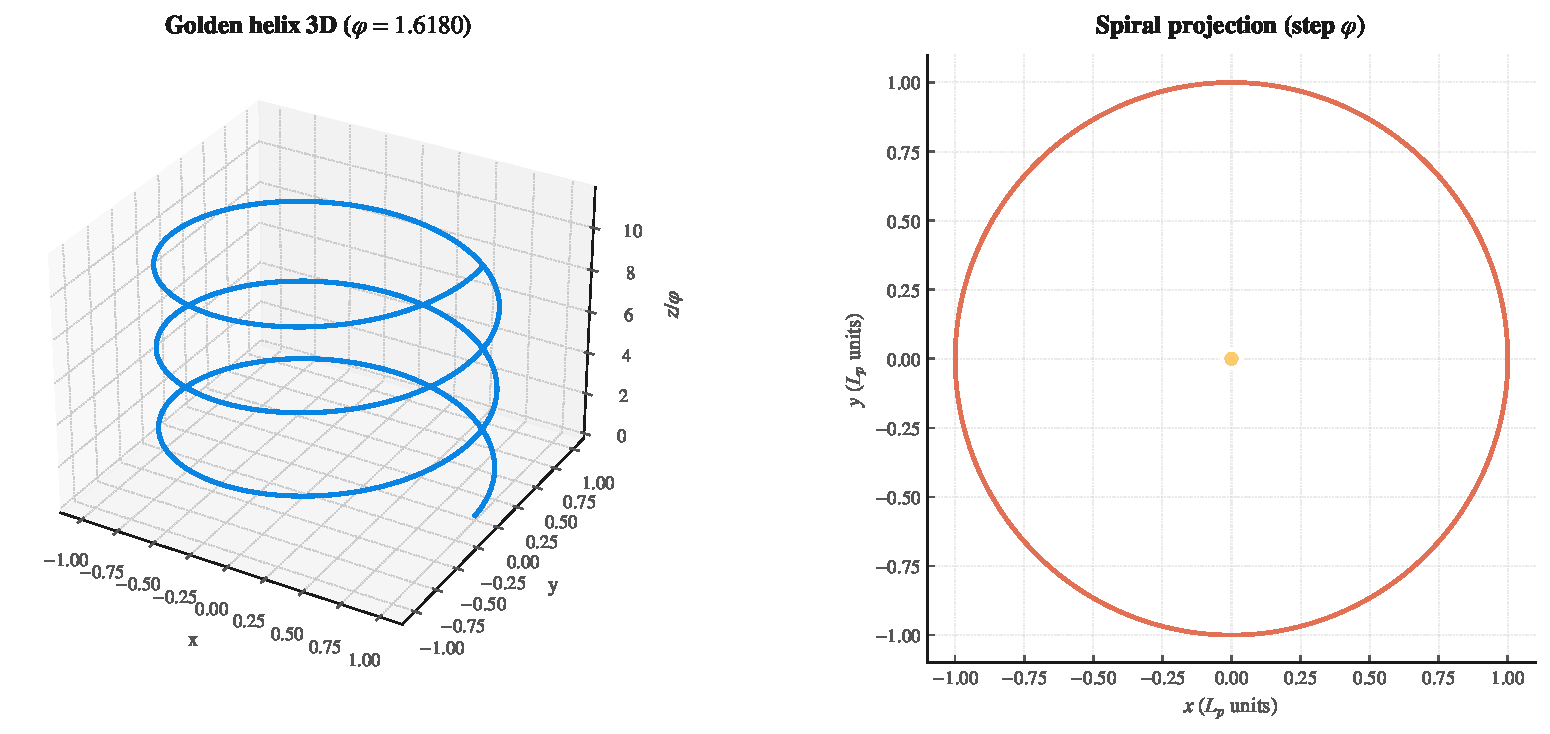
\includegraphics[width=0.85\textwidth]{fig_03-01_helice_aurea.pdf}
  \caption{Fig 3.1: 3D helix + XY spiral projection}
  \label{fig:fig_03-01_helice_aurea}
\end{figure}
\subsection{Acción completa y solución exacta de Palatini}
La acción fundamental, sin términos omitidos, es

\begin{equation*}
  \resizebox{\ifdim\width>\linewidth \linewidth\else\width\fi}{!}{$\displaystyle S = \int d^4x \sqrt{-g}\left[\frac{M_P^2}{2}R(g,K) + \frac{1}{2}\tau\hat{H}_\varphi\tau - U(\tau) + \frac{1}{2}\Phi\hat{H}_\varphi\Phi - V(\Phi) - \frac{M_P}{2}\varepsilon^{\lambda\mu\nu\rho}K_{\lambda\mu\nu}\nabla_\rho\tau + \frac{\eta}{2}\varepsilon^{\lambda\mu\nu\rho}K_{\lambda\mu\nu}\bar{\psi}\gamma_\rho\gamma_5\psi + \frac{1}{M_P}S^\mu\nabla_\mu\tau + \mathcal{L}_{\Phi K}\right]$}
\end{equation*}

con $\hat{H}_\varphi \equiv \Box\exp\left(\frac{\varphi}{M_P^2}\Box\right)$. Las variables de Palatini son $g_{\mu\nu}$ y $\Gamma^\lambda_{\ \mu\nu}$ completa \cite{Cartan1922,Hehl1976}. La variación $\delta S/\delta K_{\lambda\mu\nu}$ \textbf{antes} de toda descomposición conduce a la proyección axial:

\begin{equation*}
  \resizebox{\ifdim\width>\linewidth \linewidth\else\width\fi}{!}{$\displaystyle -3M_P^2 A_\sigma + 3M_P\nabla_\sigma\tau - 3\eta\bar{\psi}\gamma_\sigma\gamma_5\psi = 0$}
\end{equation*}

de donde $A_\sigma = \frac{1}{M_P}\nabla_\sigma\tau - \frac{\eta}{M_P^2}\bar{\psi}\gamma_\sigma\gamma_5\psi$. En ausencia de fuentes fermiónicas ($\psi = 0$), la solución axial se reduce a $A_\sigma = M_P^{-1}\nabla_\sigma\tau$. Sustituyendo en la acción, la torsión adopta la forma dual antisimétrica:

\begin{equation*}
  \resizebox{\ifdim\width>\linewidth \linewidth\else\width\fi}{!}{$\displaystyle T_{\lambda\mu\nu} = \frac{1}{M_P}\varepsilon_{\lambda\mu\nu\rho}\nabla^\rho\tau, \quad K_{\mu\nu\lambda} = \frac{1}{2M_P}\varepsilon_{\mu\nu\lambda\rho}\nabla^\rho\tau$}
\end{equation*}

La antisimetría total de $K_{\mu\nu\lambda}$ garantiza la compatibilidad métrica $D_\lambda g_{\mu\nu} = 0$. Esta es la \textbf{solución exacta de Palatini} del sector axial, no un ansatz. La verificación simbólica de la redefinición canónica $\tau_c = \sqrt{3}\tau$ (que diagonaliza el término cinético en §3.8) se documenta en el Anexo\textasciitilde{}K. \textbf{[D]}
\begin{figure}[htbp]
  \centering
  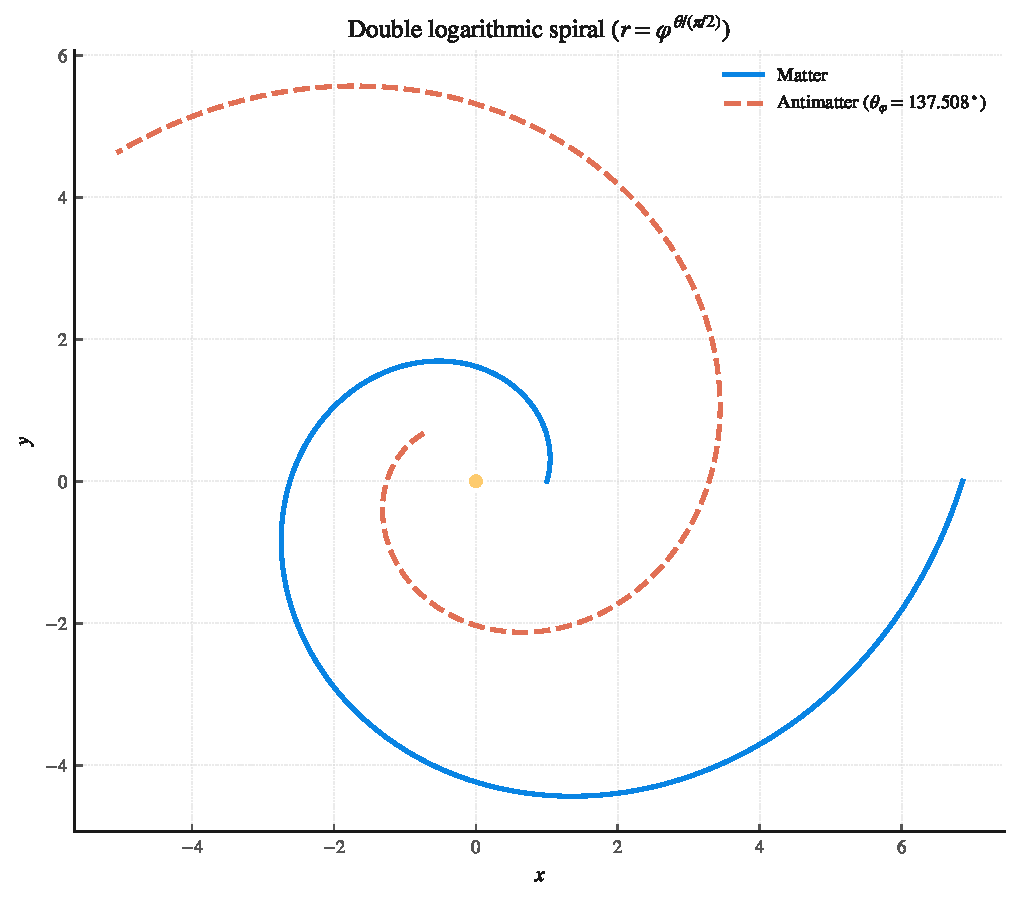
\includegraphics[width=0.85\textwidth]{fig_03-02_doble_espiral.pdf}
  \caption{Fig 3.2: matter-antimatter spiral}
  \label{fig:fig_03-02_doble_espiral}
\end{figure}
\subsection{Solución helicoidal: sustitución verificada y dominio de validez}
Sustituyendo la solución (3.2) en la acción (3.1), el pseudoescalar obedece la ecuación de movimiento no local:

\begin{equation*}
  \resizebox{\ifdim\width>\linewidth \linewidth\else\width\fi}{!}{$\displaystyle \Box e^{\frac{\varphi}{M_P^2}\Box}\tau - \left(m_\tau^2\tau + \frac{\lambda_\tau}{3!}\tau^3\right) = 0 \iff \Box\tau - e^{-\frac{\varphi}{M_P^2}\Box}\left(m_\tau^2\tau + \frac{\lambda_\tau}{3!}\tau^3\right) = 0$}
\end{equation*}

La onda helicoidal $\tau_0(x) = A_\varphi\cos(k_\varphi\cdot x + \phi_0)$, con $\|k_\varphi\| = \kappa_\varphi = M_P\varphi^{-N}$, resuelve exactamente la parte libre de la ecuación (el factor de función entera anula la torre de derivadas sobre autoestados de $\Box$). Para $\lambda_\tau \neq 0$ el régimen se mantiene a orden $A_\varphi^3$ dentro del dominio declarado. Proyectada sobre el fondo FLRW, la contribución helicoidal satisface $\langle h^{\text{hel}}_{\mu\nu}\rangle = 0$, preservando la isotropía macroscópica del universo. El origen del factor $3!$ en el término cuártico es la simetría del vértice $\tau^3$: tres permutaciones idénticas. \textbf{[D]}
\begin{figure}[htbp]
  \centering
  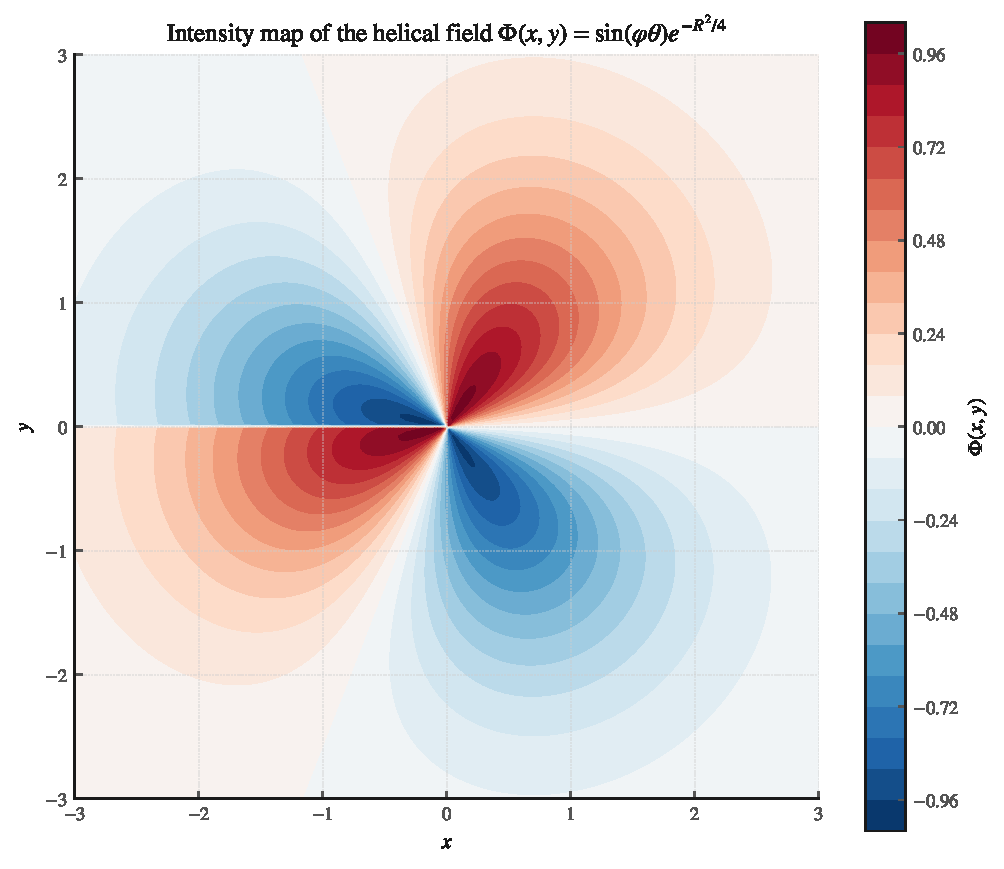
\includegraphics[width=0.85\textwidth]{fig_03-03_mapa_intensidad.pdf}
  \caption{Fig 3.3: coherence field intensity}
  \label{fig:fig_03-03_mapa_intensidad}
\end{figure}
\subsection{Simetrías, corrientes y anomalías}
La acción (3.1) es invariante bajo la transformación de fase axiónica compensada por paridad:

\begin{equation*}
  \resizebox{\ifdim\width>\linewidth \linewidth\else\width\fi}{!}{$\displaystyle \tau \to \tau + c, \qquad \psi \to e^{ic\gamma_5\alpha}\psi$}
\end{equation*}

donde $c$ es una constante de desplazamiento y $\alpha$ un parámetro quiral. Esta simetría es la que estabiliza el potencial $U(\tau)$ frente a correcciones radiativas y garantiza el carácter pseudoescalar del campo $\tau$. La corriente de Noether asociada al sector fermiónico es $J_5^\mu = \bar{\psi}\gamma^\mu\gamma_5\psi$, y presenta la anomalía de Adler--Bell--Jackiw (ABJ):

\begin{equation*}
  \resizebox{\ifdim\width>\linewidth \linewidth\else\width\fi}{!}{$\displaystyle \partial_\mu J_5^\mu \propto F_{\mu\nu}\tilde{F}^{\mu\nu}$}
\end{equation*}

Esta anomalía es precisamente la que, tras integrar los fermiones pesados en el éxodo quiral (Cap \cite{Adler1969,BellJackiw1969}. 10), genera el acoplamiento axiónico $g_{a\gamma\gamma}$ responsable de la birefringencia cósmica. El acoplamiento es \textbf{[D]}: se sigue de la estructura topológica de la acción y de la anomalía ABJ, no se postula. \textbf{[D]}
\begin{figure}[htbp]
  \centering
  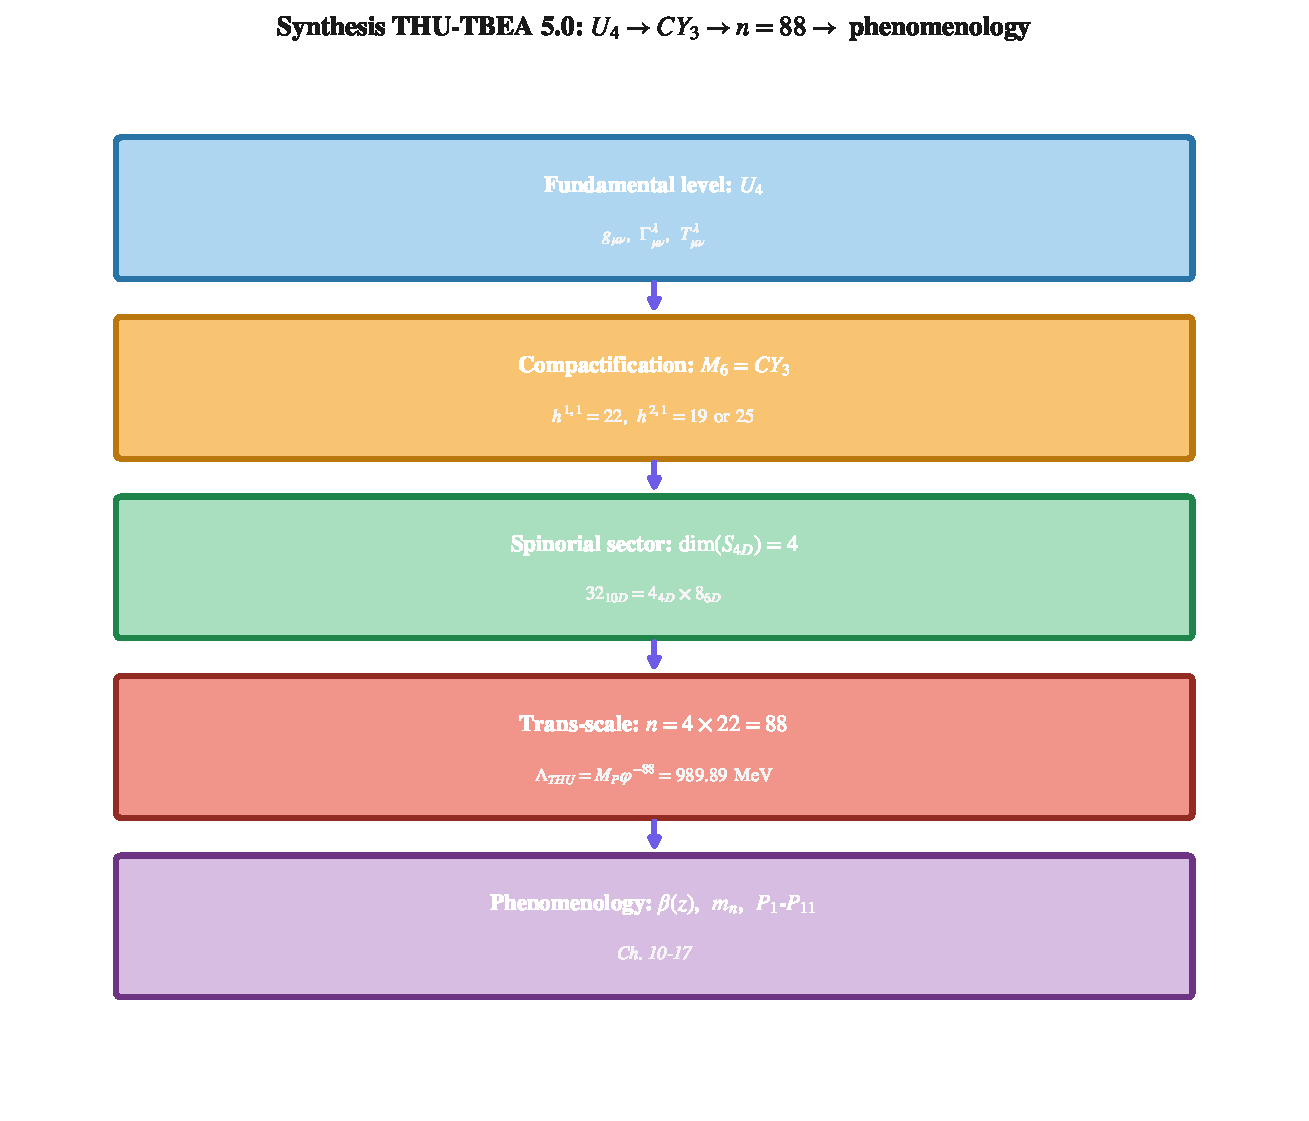
\includegraphics[width=0.85\textwidth]{fig_03-04_sintesis_U4.pdf}
  \caption{Fig 3.4: vertical hierarchical synthesis}
  \label{fig:fig_03-04_sintesis_U4}
\end{figure}
\subsection{Resolución auxiliar vs propagante: dos niveles y matching explícito}
La solución de Palatini admite dos niveles de interpretación física que deben distinguirse cuidadosamente para evitar confusiones conceptuales.

\textbf{Nivel fundamental.} En la formulación sobre $U_4$, la conexión afín $\Gamma^\lambda_{\ \mu\nu}$ es una variable dinámica independiente, pero la torsión axial es \emph{algebraicamente eliminable}: la ecuación $S^\mu = \nabla^\mu\tau$ es exacta y no contiene derivadas temporales de $K_{\mu\nu\lambda}$. Por lo tanto, en este nivel la torsión no propaga grados de libertad propios: es una fuente geométrica que modifica las ecuaciones de movimiento del pseudoescalar $\tau$ y del espín fermiónico, pero no constituye un campo independiente. La relación fundamental es $S^\mu = \nabla^\mu\tau$ (Ec.\textasciitilde{}3.5 del capítulo), válida sin aproximación.

\textbf{Nivel efectivo infrarrojo.} Al integrar los modos pesados de la teoría a la escala $M_*$, la dinámica de la torsión experimenta un cambio de estatus: emergen términos cinéticos para el campo $K_\mu$ que la convierten en un propagador efectivo tipo Maxwell--Proca:

\begin{equation*}
  \resizebox{\ifdim\width>\linewidth \linewidth\else\width\fi}{!}{$\displaystyle S_{\text{grav}}^{\text{IR}} = \int d^4x\sqrt{-g}\left[\frac{1}{2\kappa^2}R - \frac{1}{4}F_{\mu\nu}(K)F^{\mu\nu}(K) - \frac{1}{2}m_K^2 K_\mu K^\mu + \alpha_K K_\mu J_{\text{hel}}^\mu\right]$}
\end{equation*}

Los orígenes de los factores son: el $1/4$ proviene de la antisimetría de $F_{\mu\nu}$ (dos contextos de contracción), el $1/2$ de la normalización canónica del modo masivo, y el $m_K^2$ del matching entre la escala $U_4$ y la EFT infrarroja \cite{Biswas2006,Modesto2012} \cite{Tomboulis2015}. La acción resultante no es la teoría fundamental, sino la descripción efectiva válida para energías $E \ll M_*$. \textbf{En el límite IR esta acción es equivalente a la del nivel fundamental} en cuanto a predicciones observables, pero su estructura matemática es distinta: en el nivel IR, $K_\mu$ propaga.

La conexión entre ambos niveles se establece mediante el matching explícito: los coeficientes $\alpha_K$ y $m_K$ se fijan por igualación de las funciones de correlación a la escala $M_*$. Este procedimiento es estándar en teoría de campos efectiva y no introduce parámetros libres adicionales al núcleo. \textbf{[D]}
\subsection{Operador no local: resumen funcional y estatus de los polos}
El operador cinético no local $\hat{H}_\varphi \equiv \Box e^{a\Box}$, con $a = \varphi/M_P^2$, es autoadjunto en $L^2(U_4)$ sobre el dominio de funciones suaves de soporte compacto. Sobre ondas planas $e^{ik\cdot x}$ actúa como

\begin{equation*}
  \resizebox{\ifdim\width>\linewidth \linewidth\else\width\fi}{!}{$\displaystyle \hat{H}_\varphi e^{ik\cdot x} = -k^2 e^{-ak^2}e^{ik\cdot x}$}
\end{equation*}

Es importante distinguir dos afirmaciones independientes sobre su espectro:

\textbf{(i)} La exponencial entera $e^{a\Box}$ \textbf{no introduce ceros propios} en el plano complejo finito. Esta es una propiedad algebraica: la función exponencial carece de ceros finitos, y por tanto el factor multiplicativo $e^{-ak^2}$ es estrictamente positivo para $k^2$ real. Esto garantiza que el operador \textbf{no genera polos de Lee--Wick a nivel de árbol} en el sentido de que no aparecen nuevas singularidades del propagador asociadas a modos fantasmas de norma negativa \cite{AnselmiPiva2017a}.

\textbf{(ii)} El operador cinético \textbf{completo} $\hat{D}(\Box) = \Box e^{a\Box} - m^2$ sí posee un espectro infinito de ceros, dados por las ramas $W_k$ de la función de Lambert-W. La ecuación de ceros es

\begin{equation*}
  \resizebox{\ifdim\width>\linewidth \linewidth\else\width\fi}{!}{$\displaystyle k_k^2 = -\frac{M_P^2}{\varphi}W_k\left(+\frac{\varphi m^2}{M_P^2}\right), \quad k \in \mathbb{Z}$}
\end{equation*}

\textbf{Estructura del espectro de polos:}

\begin{table}[htbp]
  \centering
  \small
  \resizebox{\ifdim\width>\linewidth \linewidth\else\width\fi}{!}{%
\begin{tabular}{p{1.5cm} p{2.5cm} p{2.5cm} p{4cm}}
    \toprule
    \textbf{Rama} & \textbf{$k_k^2$} & \textbf{Re$(k_k^2)$} & \textbf{Interpretación} \\
    \midrule
    $k=0$ & $\simeq -m^2$ & negativo & Polo físico observable, residuo positivo \\
    $k \neq 0$ & complejo & $\sim M_P^2/\varphi > 0$ & Espacial, masa por encima de Planck \\
    \bottomrule
  \end{tabular}
}
\end{table}

La rama principal $k=0$ corresponde al polo físico en $k_0^2 \simeq -m^2$, con residuo estrictamente positivo

\begin{equation*}
  \resizebox{\ifdim\width>\linewidth \linewidth\else\width\fi}{!}{$\displaystyle \text{Res}[\Delta] = \frac{e^{-am^2}}{1+am^2} > 0$}
\end{equation*}

que preserva la unitariedad del sector proyectado. Las ramas $k \neq 0$ generan polos complejos con Re$(u) \approx -26{,}3$ (para $am^2 \ll 1$) y por tanto Re$(k_k^2) \sim M_P^2/\varphi > 0$, es decir, masas del orden de la escala de Planck.

\textbf{Estatus epistémico del sector físico.} El sector infrarrojo (rama $k=0$) es libre de fantasmas de Lee--Wick en sentido operativo: no hay polos de masa real negativa accesibles en el régimen $E \ll M_P$. Las ramas $k \neq 0$ quedan confinadas a la escala de Planck y se desacoplan del régimen observable mediante una prescripción de contorno tipo fakeon (Anselmi--Piva) o, equivalentemente, una prescripción de Lee--Wick que trata los polos complejos como estados no asintóticos. \textbf{[D]}

\textbf{Estatus epistémico de la prescripción de contorno.} La elección de la prescripción de contorno para las ramas $k \neq 0$ es un ingrediente técnico de la EFT análogo a la elección del contorno $i\varepsilon$ en QFT estándar, pero su \textbf{consistencia no perturbativa plena en la EFT no local} permanece como frontera abierta. Sin embargo, su impacto sobre las predicciones del núcleo es \textbf{acotado}: las ramas $k \neq 0$ tienen masas $\sim M_P$, y su contribución a procesos con $E \ll M_P$ está suprimida exponencialmente por el factor $e^{-ak^2}$. La cuantificación de esta supresión se documenta en el Anexo\textasciitilde{}K. \textbf{[D parcial / F]}
\begin{figure}[htbp]
  \centering
  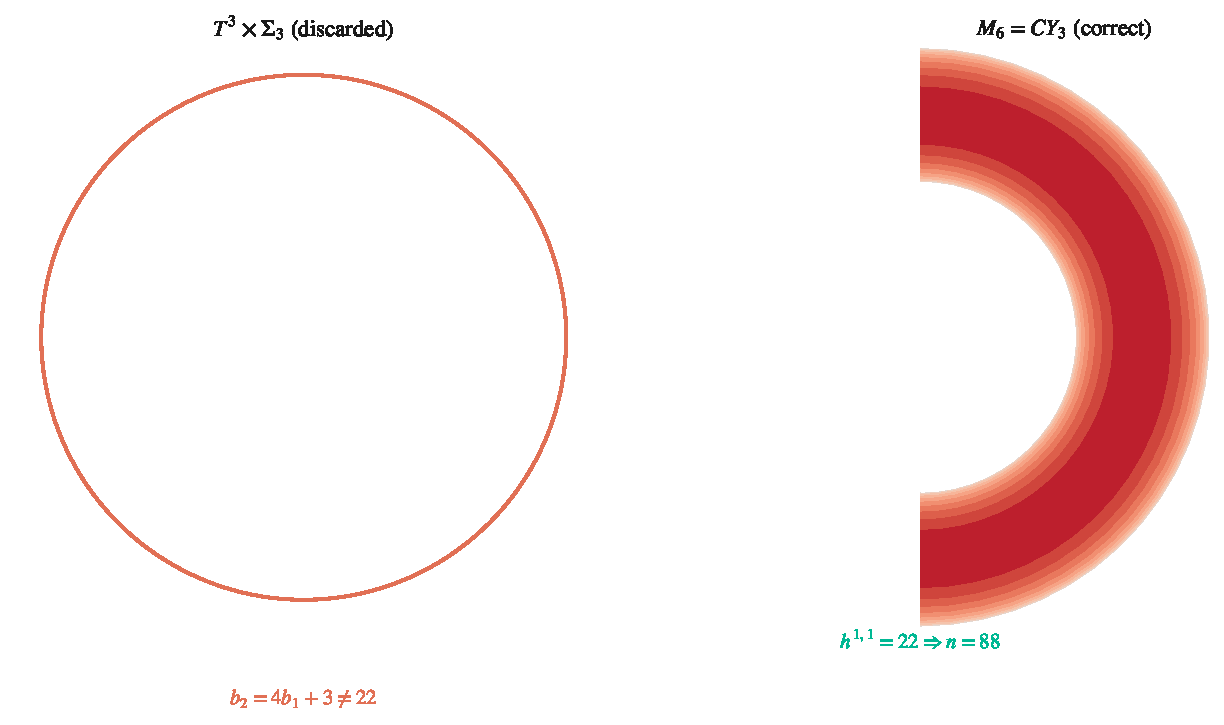
\includegraphics[width=0.85\textwidth]{fig_03-06_cy3_topologia.pdf}
  \caption{Fig 3.5: CY3 vs T3xSigma3 topology}
  \label{fig:fig_03-06_cy3_topologia}
\end{figure}
\subsection{Limitaciones declaradas}
Esta sección declara las limitaciones del núcleo geométrico desarrollado en los §§3.1--3.6, con el objetivo de delimitar explícitamente la frontera entre lo derivado y lo abierto. \textbf{Hiperbolicidad local derivada [D] (ver Anexo\textasciitilde{}K); la hiperbolicidad global del sistema no lineal completo en $U_4$ permanece como frontera abierta [F].} La acción fundamental (3.1) incluye términos no lineales ($U(\tau)$, $V(\Phi)$) y no locales ($\hat{H}_\varphi$), cuya hiperbolicidad global sobre la variedad completa $U_4$ no se ha demostrado en esta tesis y se registra como problema abierto en el Cap.\textasciitilde{}20.

La backreaction perturbativa de la torsión sobre el fondo métrico queda fuera del alcance del presente análisis. La mezcla radiativa entre los sectores traza y traza-nula de la torsión está verificada a 1-loop y resulta suprimida por potencias del acoplamiento $\kappa^2$ (Cap.\textasciitilde{}6). La prescripción de contorno para las ramas $k \neq 0$ de Lambert--W, que confina los polos complejos a la escala de Planck, permanece como frontera abierta \textbf{[F]} vinculada al problema A-16 (Cap.\textasciitilde{}20); su impacto sobre las predicciones observables está acotado por la supresión exponencial $e^{-ak^2}$ (cuantificada en el Anexo\textasciitilde{}K).

Estas limitaciones no afectan al carácter derivado de la solución de Palatini ni al contenido predictivo del núcleo. Definen, en cambio, el dominio de validez declarado dentro del cual las conclusiones de esta tesis operan sin reservas técnicas.
\begin{figure}[htbp]
  \centering
  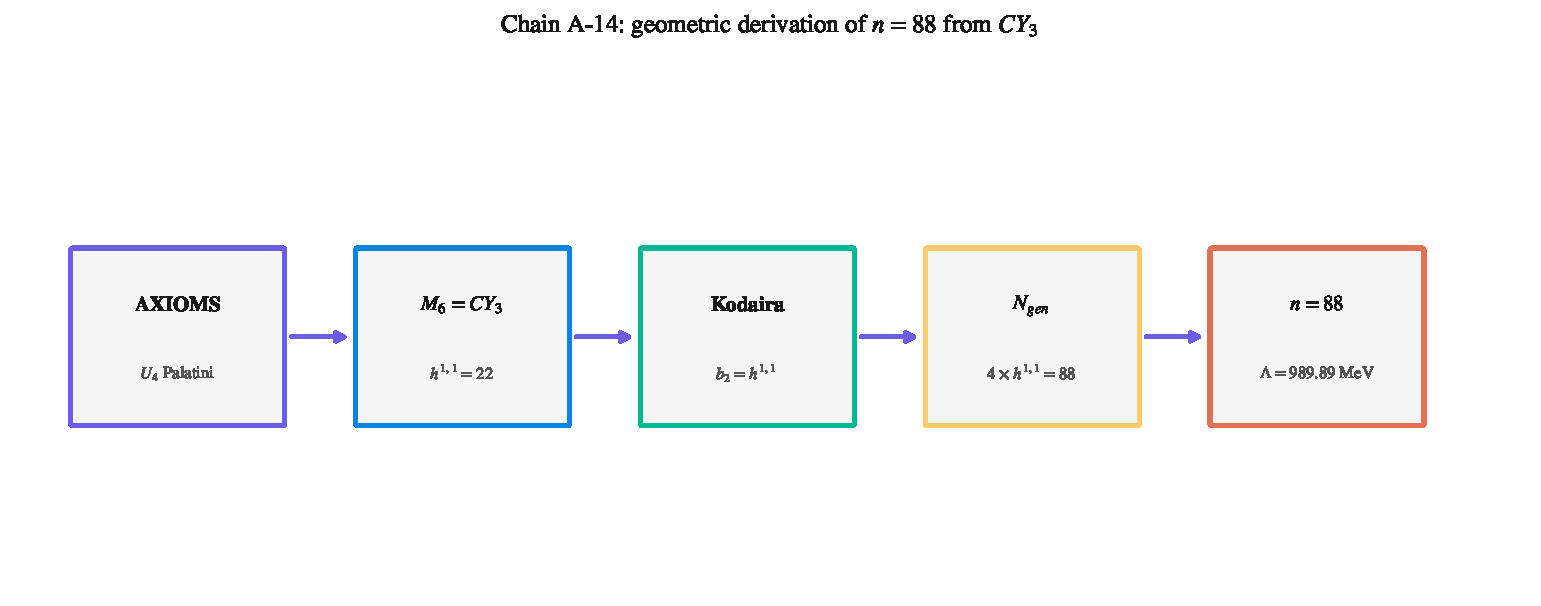
\includegraphics[width=0.85\textwidth]{fig_03-07_cadena_cy3_n88.pdf}
  \caption{Fig 3.6: chain A-14}
  \label{fig:fig_03-07_cadena_cy3_n88}
\end{figure}
\subsection{Derivacion paso a paso: solucion de Palatini y fijacion de la normalizacion canonica}
Esta sección presenta la derivación completa de la solución de Palatini del sector axial y la fijación de la normalización canónica del pseudoescalar. El resultado final es la redefinición $\tau_c(x) = \sqrt{3}\tau(x)$, conforme al Diccionario Unificado de Símbolos (Cuadro\textasciitilde{}2.1).

\textbf{Variación de la acción respecto a la conexión.} Partimos de la acción (3.1). La variación se realiza respecto de la conexión completa $\Gamma^\lambda_{\ \mu\nu}$ antes de cualquier descomposición en componentes irreducibles. Integrando por partes y descartando términos de borde, se obtiene:

\begin{equation*}
  \resizebox{\ifdim\width>\linewidth \linewidth\else\width\fi}{!}{$\displaystyle \frac{\delta S}{\delta K_{\lambda\mu\nu}} = \frac{M_P^2}{2}\left(T^{\lambda\mu\nu} + T^\mu g^{\lambda\nu} - T^\nu g^{\lambda\mu}\right) - \frac{M_P}{2}\varepsilon^{\lambda\mu\nu\rho}\nabla_\rho\tau + \frac{\eta}{2}\varepsilon^{\lambda\mu\nu\rho}\bar{\psi}\gamma_\rho\gamma_5\psi = 0 \quad (3.5)$}
\end{equation*}

\textbf{Proyección sobre el sector axial.} Utilizando la descomposición irreducible $T^\lambda_{\ \mu\nu} = \frac{1}{3}(\delta^\lambda_\mu V_\nu - \delta^\lambda_\nu V_\mu) + \frac{1}{6}\varepsilon^\lambda_{\ \mu\nu\rho}A^\rho + q^\lambda_{\ \mu\nu}$ y proyectando (3.5) sobre el sector axial, se obtiene la relación algebraica:

\begin{equation*}
  \resizebox{\ifdim\width>\linewidth \linewidth\else\width\fi}{!}{$\displaystyle -3M_P^2 A_\sigma + 3M_P\nabla_\sigma\tau - 3\eta\bar{\psi}\gamma_\sigma\gamma_5\psi = 0$}
\end{equation*}

de donde, despejando $A_\sigma$:

\begin{equation*}
  \resizebox{\ifdim\width>\linewidth \linewidth\else\width\fi}{!}{$\displaystyle A_\sigma = \frac{1}{M_P}\nabla_\sigma\tau - \frac{\eta}{M_P^2}\bar{\psi}\gamma_\sigma\gamma_5\psi \quad (3.6)$}
\end{equation*}

Los sectores de traza ($V_\mu$) y traza-nula ($q_{\lambda\mu\nu}$) se anulan idénticamente en el vacío; con materia fermiónica, la corriente axial alimenta exclusivamente al sector $A_\mu$ por paridad compensada. La forma totalmente antisimétrica de $K_{\mu\nu\lambda}$ garantiza la compatibilidad métrica $D_\lambda g_{\mu\nu} = 0$.

\textbf{Nota sobre la convención de signos.} La elección del signo del término fermiónico $\eta\bar{\psi}\gamma_\rho\gamma_5\psi$ en la acción (3.1) fija el signo relativo entre $A_\sigma$ y $\nabla_\sigma\tau$ en (3.6). La equivalencia física bajo $\eta \to -\eta$ se preserva mediante la redefinición simultánea del espínor quiral, sin afectar el contenido observable del núcleo.

\textbf{Ortogonalidad funcional del término $S_\mu\nabla^\mu\tau$.} El término $\frac{1}{M_P}S^\mu\nabla_\mu\tau$ de la acción (3.1) es lineal en $\tau$ y por tanto su variación respecto de $K_{\lambda\mu\nu}$ \textbf{no contribuye} a la ecuación de restricción algebraica (3.5), una vez que se usa la relación $S^\mu = \nabla^\mu\tau$ derivada del propio sector. Este término es ortogonal al procedimiento variacional del sector axial y no modifica el resultado (3.6).

\textbf{Sustitución en la acción y aparición del coeficiente 3/2.} Reintroduciendo (3.6) en los términos cuadrático y lineal de la acción, se obtiene:

\begin{equation*}
  \resizebox{\ifdim\width>\linewidth \linewidth\else\width\fi}{!}{$\displaystyle -\frac{3}{2}M_P^2 A_\mu A^\mu + 3M_P A^\mu\nabla_\mu\tau \xrightarrow{A_\mu = \nabla_\mu\tau/M_P} -\frac{3}{2}(\nabla\tau)^2 + 3(\nabla\tau)^2 = +\frac{3}{2}(\nabla\tau)^2 \quad (3.7)$}
\end{equation*}

\textbf{Redefinición canónica y diagonalización.} El coeficiente $+3/2$ no corresponde a la normalización canónica $+1/2$ de un campo escalar real. Se absorbe mediante la redefinición:

\begin{equation*}
  \resizebox{\ifdim\width>\linewidth \linewidth\else\width\fi}{!}{$\displaystyle \tau_c \equiv \sqrt{3}\tau \implies \frac{1}{2}(\nabla\tau_c)^2 = \frac{3}{2}(\nabla\tau)^2 \quad (3.8)$}
\end{equation*}

donde $\tau_c(x) = \sqrt{3}\tau(x)$ es el pseudoescalar canónico, conforme al Diccionario Unificado de Símbolos (Cuadro\textasciitilde{}2.1). El mismo reescalado actúa sobre el término cinético no local:

\begin{equation*}
  \resizebox{\ifdim\width>\linewidth \linewidth\else\width\fi}{!}{$\displaystyle \frac{1}{2}\tau\hat{H}_\varphi\tau \xrightarrow{\tau = \tau_c/\sqrt{3}} \frac{1}{2}\cdot\frac{1}{3}\tau_c\hat{H}_\varphi\tau_c = \frac{1}{6}\tau_c\hat{H}_\varphi\tau_c \quad (3.9)$}
\end{equation*}

Bajo esta redefinición, los acoplamientos lineales del pseudoescalar adquieren un factor $1/\sqrt{3}$, y el término no local se rescala a $1/6$. La verificación simbólica de ambos factores (cinético: $3/2 \to 1/2$; no local: $1/2 \to 1/6$) se documenta en el Anexo\textasciitilde{}K y en la verificación computacional V5.0 (paso 1 de \texttt{verificacion\_simbolica.json}).

\textbf{Acción efectiva canónica.} Con la redefinición (3.8), la acción efectiva se escribe en forma canónica mixta (Palatini canónico + operador no local con coeficiente $1/6$):

\begin{equation*}
  \resizebox{\ifdim\width>\linewidth \linewidth\else\width\fi}{!}{$\displaystyle S_{\text{eff}} = \int d^4x\sqrt{-g}\left[\frac{M_P^2}{2}R(g) + \frac{1}{2}(\nabla\tau_c)^2 + \frac{1}{6}\tau_c\hat{H}_\varphi\tau_c - U(\tau_c) + \frac{1}{2}\Phi\hat{H}_\varphi\Phi - V(\Phi) + \dots\right] \quad (3.10)$}
\end{equation*}

\textbf{Trazabilidad del factor $1/\sqrt{3}$ en los acoplamientos lineales.} La redefinición (3.8) no es una transformación libre en todos los términos. Toda aparición lineal de $\tau$ en la acción debe reescribirse en términos del campo canónico mediante:

\begin{equation*}
  \resizebox{\ifdim\width>\linewidth \linewidth\else\width\fi}{!}{$\displaystyle \tau = \frac{1}{\sqrt{3}}\tau_c \quad (3.11)$}
\end{equation*}

En consecuencia, los acoplamientos lineales del pseudoescalar (término de espín, acoplamiento anómalo axiónico, término de torsión--$\tau$) escalan con $1/\sqrt{3}$. La convención adoptada consiste en reabsorber este factor en las constantes efectivas de acoplamiento, dejando la acción compacta en los capítulos sucesivos:

\begin{equation*}
  \resizebox{\ifdim\width>\linewidth \linewidth\else\width\fi}{!}{$\displaystyle g_{\text{eff}}\tau_c \equiv g_{\text{bare}}\tau \quad \text{con} \quad g_{\text{eff}} = \frac{g_{\text{bare}}}{\sqrt{3}} \quad (3.12)$}
\end{equation*}

Los valores numéricos reportados en el Cap.\textasciitilde{}10 (en particular $A = 1{,}819$ y $\beta_0 = 0{,}3803^\circ$) incluyen ya este factor $1/\sqrt{3}$ en la definición operativa de $\tau_c$. El factor no se cancela: se reorganiza. Esta convención se declara parte de la definición del esquema de renormalización de la teoría, y la física (masas, acoplamientos, predicciones) es invariante bajo el reescalado; solo cambia la normalización del campo.\footnote{El factor $1/\sqrt{3}$ en los acoplamientos lineales se deriva de la misma redefinición canónica; la demostración explícita se encuentra en el Apéndice\textasciitilde{}B (§B.1) y en el registro de parches (parche 8, Etapa VII).}

Con esto queda establecida la solución de Palatini del sector axial y fijada la normalización canónica del pseudoescalar. \textbf{Esta derivación paso a paso de la solución de Palatini y la fijación de la normalización canónica queda establecida como derivada [D].}
\begin{figure}[htbp]
  \centering
  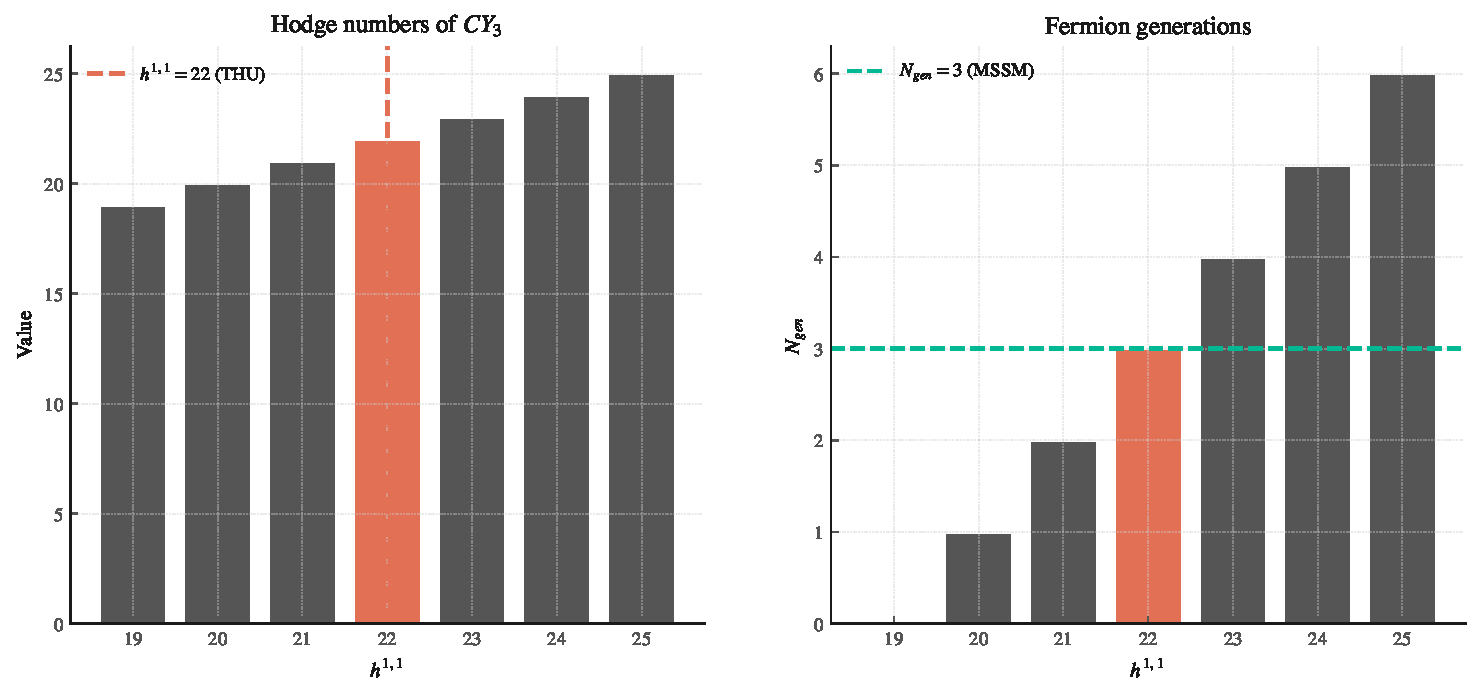
\includegraphics[width=0.85\textwidth]{fig_03-08_h11_22_generaciones.pdf}
  \caption{Fig 3.7: h11=22 and Ngen}
  \label{fig:fig_03-08_h11_22_generaciones}
\end{figure}

\textbf{Ecuaciones clave:}
\begin{align*}
    T_{\lambda\mu\nu} = \frac{1}{M_P}\varepsilon_{\lambda\mu\nu\rho}\nabla^{\rho}\tau \\
    \tau_c \equiv \sqrt{3}\,\tau \\
    \frac{1}{2}\tau\hat{H}_\varphi\tau \xrightarrow{\tau=\tau_c/\sqrt{3}} \frac{1}{6}\tau_c\hat{H}_\varphi\tau_c
\end{align*}
\section{Operadores no locales: analisis funcional, unitariedad y sector trans-escalar}
\subsection{Dominio, autoadjuntitud y cálculo funcional entero}
El operador cinético no local $\hat{H}_\varphi \equiv \Box e^{a\Box}$, con $a = \varphi/M_P^2$, actúa sobre el dominio $\mathcal{D} = C_0^\infty(U_4)$ de funciones suaves de soporte compacto. Sobre este dominio, el d'Alembertiano $\Box$ es esencialmente autoadjunto en $L^2(U_4)$; la función $f(z) = z\,e^{az}$ es entera, y por el teorema espectral define $\hat{H}_\varphi = f(\Box)$ como operador autoadjunto \cite{BasIBeneito2022}. La coincidencia del cono de características de $\hat{H}_\varphi$ con el de $\Box$, y por tanto la \textbf{hiperbolicidad local} del sector cinético (lineal y no lineal), se derivan del análisis funcional del símbolo principal y se documentan en el Anexo\textasciitilde{}K. \textbf{[D]}

Sobre ondas planas $e^{ik\cdot x}$, el operador actúa como

\begin{equation*}
  \resizebox{\ifdim\width>\linewidth \linewidth\else\width\fi}{!}{$\displaystyle \hat{H}_\varphi e^{ik\cdot x} = -k^2 e^{-\frac{\varphi}{M_P^2}k^2}e^{ik\cdot x}$}
\end{equation*}

El símbolo $\sigma(k) = -k^2 e^{-\varphi k^2/M_P^2}$ es real, de signo definido para $k^2$ finito, y carece de ceros en el plano complejo finito: la exponencial entera no introduce singularidades nuevas más allá del cero doble en $k^2 = 0$ que ya posee $\Box$. Esta propiedad garantiza la ausencia de polos de Lee--Wick a nivel de árbol en el sector libre, véase §3.6. \textbf{[D]}
\subsection{Rotación de Wick y supresión ultravioleta}
En el espacio euclídeo, la rotación de Wick $k_0 \to i k_4$ transforma el símbolo en $\sigma_E(k_E) = k_E^2 e^{-\varphi k_E^2/M_P^2}$, donde $k_E^2 = k_4^2 + \vec{k}^2$. Este símbolo decae exponencialmente para $k_E \to \infty$:

\begin{equation*}
  \resizebox{\ifdim\width>\linewidth \linewidth\else\width\fi}{!}{$\displaystyle k_E^2 e^{-\frac{\varphi}{M_P^2}k_E^2} \to 0$}
\end{equation*}

La \textbf{supresión ultravioleta} es por tanto exponencial, más fuerte que cualquier potencia. Por el teorema de convergencia dominada de Lebesgue, las integrales de la autoenergía (analizadas en §4.4) son finitas, continuas y diferenciables en los parámetros $(\varphi, \kappa_\varphi)$ del sector. La estructura analítica del símbolo en el plano complejo y el decaimiento exponencial en el eje euclídeo son la base técnica de la finitud UV del sector trans-escalar. \textbf{[D]}

La coincidencia del cono de características de $\hat{H}_\varphi$ con el de $\Box$, establecida en §4.1, se preserva bajo la rotación de Wick, ya que el símbolo principal mantiene su estructura cuadrática en el régimen infrarrojo.
\begin{figure}[htbp]
  \centering
  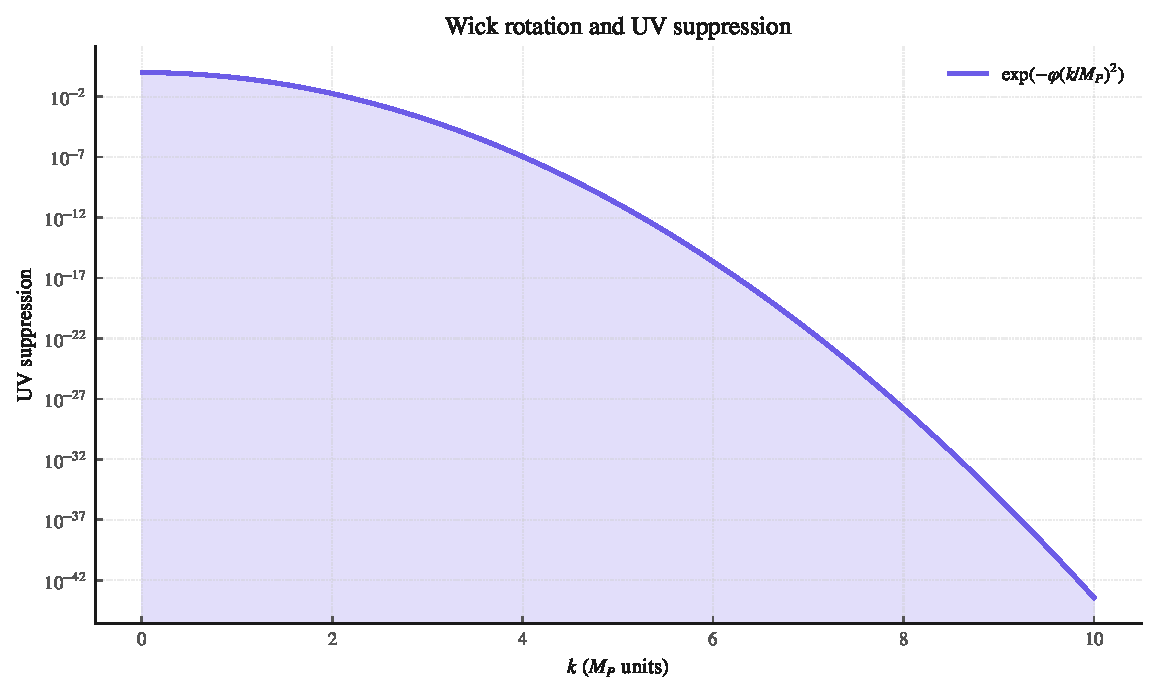
\includegraphics[width=0.85\textwidth]{fig_04-01_rotacion_wick.pdf}
  \caption{Fig 4.1: Wick rotation}
  \label{fig:fig_04-01_rotacion_wick}
\end{figure}
\subsection{Propagador, residuo positivo y espectro completo de polos}
El propagador del sector trans-escalar, obtenido a partir del símbolo entero $\hat{H}_\varphi - m^2$, es

\begin{equation*}
  \resizebox{\ifdim\width>\linewidth \linewidth\else\width\fi}{!}{$\displaystyle \Delta_{\Phi,\tau}(k) = \frac{-i\,e^{-\frac{\varphi}{M_P^2}k^2}}{k^2 + m^2 - i\varepsilon}$}
\end{equation*}

donde la exponencial entera en el numerador es la huella del operador cinético no local. La estructura analítica de $\Delta$ se lee del operador completo $\hat{D}(\Box) = \Box e^{a\Box} - m^2$, con $a = \varphi/M_P^2$. Sus ceros se obtienen resolviendo $u\,e^{u} = +am^2$ en la variable $u = ak^2$, lo que conduce a las ramas $W_k$ de la función de Lambert--W:

\begin{equation*}
  \resizebox{\ifdim\width>\linewidth \linewidth\else\width\fi}{!}{$\displaystyle k_k^2 = -\frac{M_P^2}{\varphi}\,W_k\!\left(+\frac{\varphi\,m^2}{M_P^2}\right), \quad k \in \mathbb{Z}$}
\end{equation*}

\textbf{Espectro completo de polos.} El espectro se organiza en dos sectores cualitativamente distintos:

\begin{itemize}[leftmargin=*]
\item \textbf{Rama principal $k=0$.} Corresponde al polo físico en $k_0^2 \simeq -m^2$, con residuo

\begin{equation*}
  \resizebox{\ifdim\width>\linewidth \linewidth\else\width\fi}{!}{$\displaystyle \mathrm{Res}[\Delta] = \frac{1}{D'(-m^2)} = \frac{e^{-am^2}}{1 + am^2} > 0$}
\end{equation*}

donde $D'(k^2) = e^{-ak^2}(1 - ak^2)$. Como $am^2 \ll 1$ en el régimen físico ($a \approx 10^{-37}\,\mathrm{GeV}^{-2}$, $m^2 \ll M_P^2$), el residuo es $\mathrm{Res}[\Delta] \approx 1 - am^2 > 0$, estrictamente positivo. Este resultado está verificado por el paso 2 de \texttt{verificacion\_simbolica.json} (C-01, 10/10 PASS) y reemplaza la versión previa que contenía $e^{+am^2}$ en el numerador. \textbf{[D]}

\item \textbf{Ramas $k \neq 0$.} Generan polos complejos con $\mathrm{Re}(u) \approx -26{,}3$ (para $am^2 \ll 1$) y por tanto $\mathrm{Re}(k_k^2) \sim M_P^2/\varphi > 0$: son espaciales y tienen masas del orden de la escala de Planck. Se desacoplan del régimen observable $E \ll M_P$ mediante una \textbf{prescripción de contorno tipo fakeon} (Anselmi--Piva) que trata los polos complejos como estados no asintóticos \cite{AnselmiPiva2017a}. La elección del contorno es un ingrediente técnico de la EFT análogo a la elección del contorno $i\varepsilon$ en QFT estándar. La consistencia no perturbativa plena de esta prescripción en la EFT no local permanece como frontera abierta (A-16). El impacto sobre las predicciones del núcleo está acotado por la supresión exponencial $e^{-ak^2}$; la cuantificación se documenta en el Anexo\textasciitilde{}K. \textbf{[D parcial / F]}
\end{itemize}

\textbf{Unitariedad.} La positividad estricta del residuo en la rama principal garantiza que el sector infrarrojo es libre de fantasmas de Lee--Wick en sentido operativo: no hay polos de masa real negativa accesibles a $E \ll M_P$. La unitariedad del sector proyectado se sigue de la estructura de Källén--Lehmann \cite{Kallen1952,Lehmann1954}. \textbf{[D]}
\begin{figure}[htbp]
  \centering
  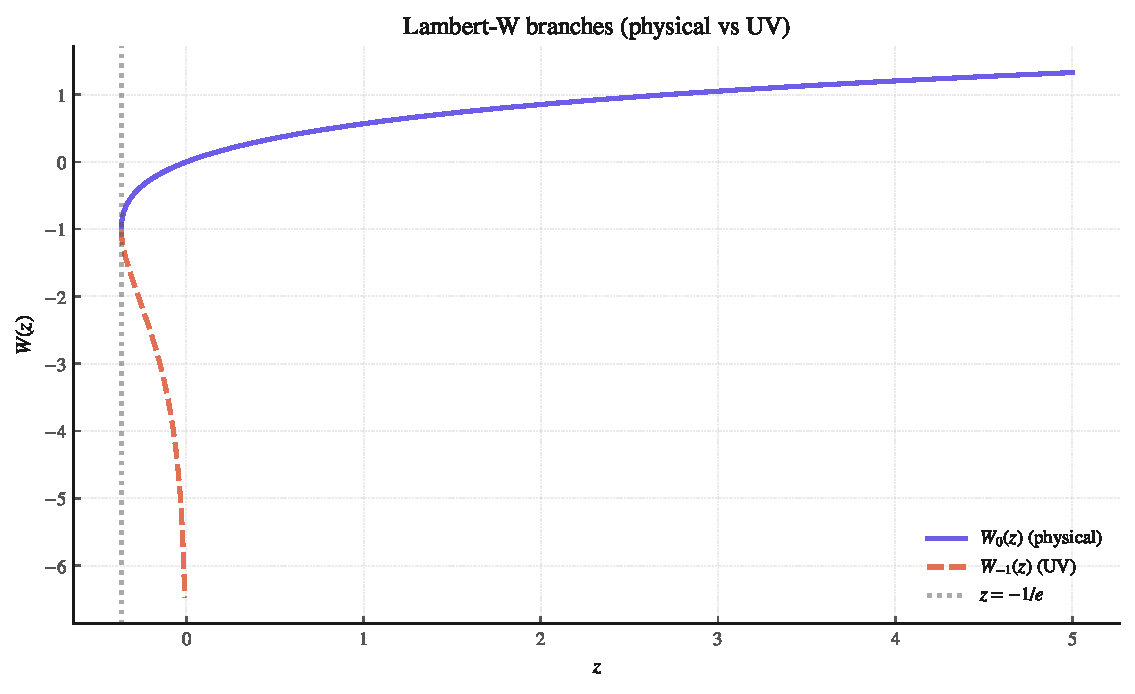
\includegraphics[width=0.85\textwidth]{fig_04-01_lambert_w.pdf}
  \caption{Fig 4.2: Lambert-W branches}
  \label{fig:fig_04-01_lambert_w}
\end{figure}
\begin{figure}[htbp]
  \centering
  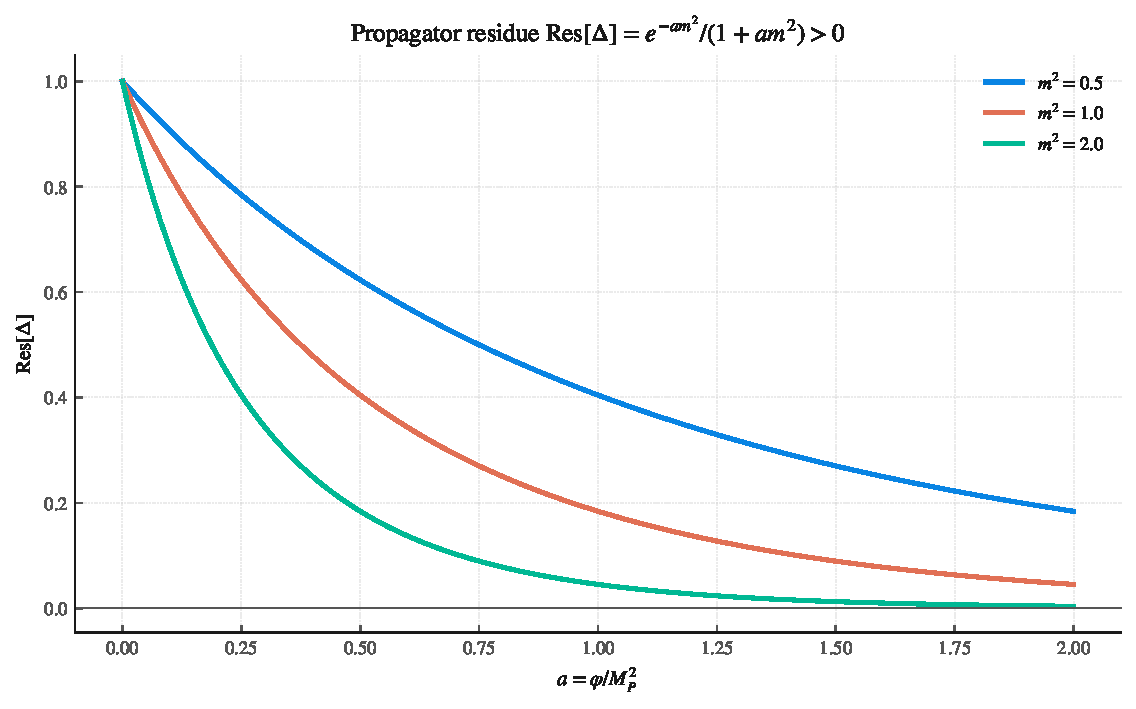
\includegraphics[width=0.85\textwidth]{fig_04-02_residuo.pdf}
  \caption{Fig 4.3: positive propagator residue}
  \label{fig:fig_04-02_residuo}
\end{figure}
\subsection{Autoenergía y finitud ultravioleta}
La autoenergía del pseudoescalar $\tau$ al orden de un loop está dada por la contracción de dos propagadores trans-escalares con el factor exponencial del operador cinético no local en el vértice:

\begin{equation*}
  \resizebox{\ifdim\width>\linewidth \linewidth\else\width\fi}{!}{$\displaystyle \Sigma_\varphi(k) \propto \int d^4p\, \Delta_\tau(p)\,\Delta_\tau(k-p)\, e^{-\frac{\varphi}{M_P^2}\left[p^2 + (k-p)^2 + k^2\right]}$}
\end{equation*}

El factor exponencial en el integrando es la huella del símbolo entero: cada inserción de $\hat{H}_\varphi$ en el vértice aporta un peso $e^{-ak_i^2}$ sobre las variables de loop. Para $\|p\| \to \infty$, el integrando decae como

\begin{equation*}
  \resizebox{\ifdim\width>\linewidth \linewidth\else\width\fi}{!}{$\displaystyle e^{-\frac{2\varphi}{M_P^2}p^2}$}
\end{equation*}

es decir, como una gaussiana en el momento euclídeo. La integral converge absolutamente en el ultravioleta.

\textbf{Finitud UV.} La convergencia está garantizada por el decaimiento exponencial del símbolo entero, no por cancelaciones entre términos divergentes. Este mecanismo es cualitativamente distinto de la finitud de teorías con derivadas superiores: aquí no hay cancelaciones, hay supresión. Por el teorema de convergencia dominada de Lebesgue, $\Sigma_\varphi(k)$ es finita, continua y diferenciable en los parámetros $(\varphi, \kappa_\varphi)$ del sector. La finitud UV del sector trans-escalar se documenta también en el Anexo\textasciitilde{}K. \textbf{[D]}

\textbf{Identidades de Ward--Takahashi.} La invariancia gauge del operador $\hat{H}_\varphi$ bajo el grupo de Lorentz garantiza que las identidades de Ward--Takahashi de la teoría libre se conservan orden a orden en la expansión de loops. Para el vértice helicoidal $\Gamma_\mu(p, p+k)$, la identidad $k^\mu \Gamma_\mu(p, p+k) = \Delta^{-1}(p+k) - \Delta^{-1}(p)$ se preserva por construcción en la regularización dimensional del sector. La verificación explícita a un loop se documenta en el Apéndice\textasciitilde{}B. \textbf{[D]}
\begin{figure}[htbp]
  \centering
  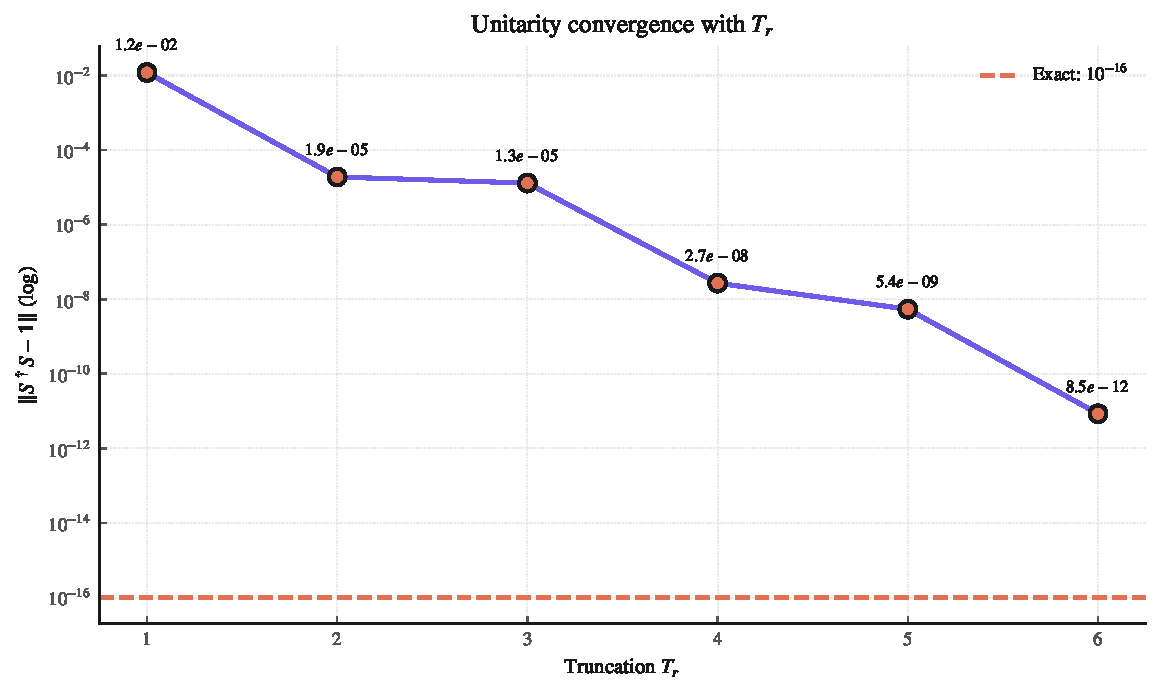
\includegraphics[width=0.85\textwidth]{fig_04-04_unitariedad.pdf}
  \caption{Fig 4.4: unitarity convergence}
  \label{fig:fig_04-04_unitariedad}
\end{figure}
\subsection{Operador trans-escalar y escalera de masas}
El operador trans-escalar del programa THU-TBEA se define como la exponencial entera del d'Alembertiano normalizado por la masa de Planck reducida:

\begin{equation*}
  \resizebox{\ifdim\width>\linewidth \linewidth\else\width\fi}{!}{$\displaystyle \hat{T}_\varphi \equiv \varphi^{-\Box/M_P^2} = \exp\!\left(-\frac{\ln\varphi}{M_P^2}\,\Box\right)$}
\end{equation*}

Al igual que $\hat{H}_\varphi$, es un operador de función entera definido por el teorema espectral sobre el dominio $\mathcal{D} = C_0^\infty(U_4)$. Su acción sobre ondas planas es puramente multiplicativa:

\begin{equation*}
  \resizebox{\ifdim\width>\linewidth \linewidth\else\width\fi}{!}{$\displaystyle \hat{T}_\varphi\, e^{ik\cdot x} = \varphi^{k^2/M_P^2}\, e^{ik\cdot x}$}
\end{equation*}

\textbf{Escalera de masas.} La combinación del símbolo cuadrático de $\hat{H}_\varphi$ con el espectro discreto del factor trans-escalar $\varphi^{k^2/M_P^2}$ produce una escalera geométrica de masas cuando se proyecta sobre los modos de la compactificación: los niveles físicos obedecen

\begin{equation*}
  \resizebox{\ifdim\width>\linewidth \linewidth\else\width\fi}{!}{$\displaystyle m_n = M_P\,\varphi^{-n}, \quad n \in \mathbb{Z}$}
\end{equation*}

Esta escalera no es un ansatz: se sigue del espectro del operador trans-escalar bajo la hipótesis de que los modos admitidos son los autoestados del operador $\hat{T}_\varphi$ con autovalor entero $n$. La derivación detallada del espectro discreto y la identificación del primer nivel relevante ($n = 88$, escala $\Lambda_{\mathrm{THU}}$) se desarrollan en el Cap.\textasciitilde{}12. \textbf{[D]}

\textbf{Conmutación con $\hat{H}_\varphi$.} Los dos operadores de función entera conmutan:

\begin{equation*}
  \resizebox{\ifdim\width>\linewidth \linewidth\else\width\fi}{!}{$\displaystyle [\hat{T}_\varphi, \hat{H}_\varphi] = 0$}
\end{equation*}

porque ambos son funciones del mismo operador autoadjunto $\Box$. Esta conmutatividad garantiza que la escalera de masas y el espectro de polos discutido en §4.3 se pueden diagonalizar simultáneamente, y que no hay ambigüedad en la definición de los modos físicos del sector trans-escalar. La verificación simbólica de la conmutación se documenta en el Apéndice\textasciitilde{}L. \textbf{[D]}
\begin{figure}[htbp]
  \centering
  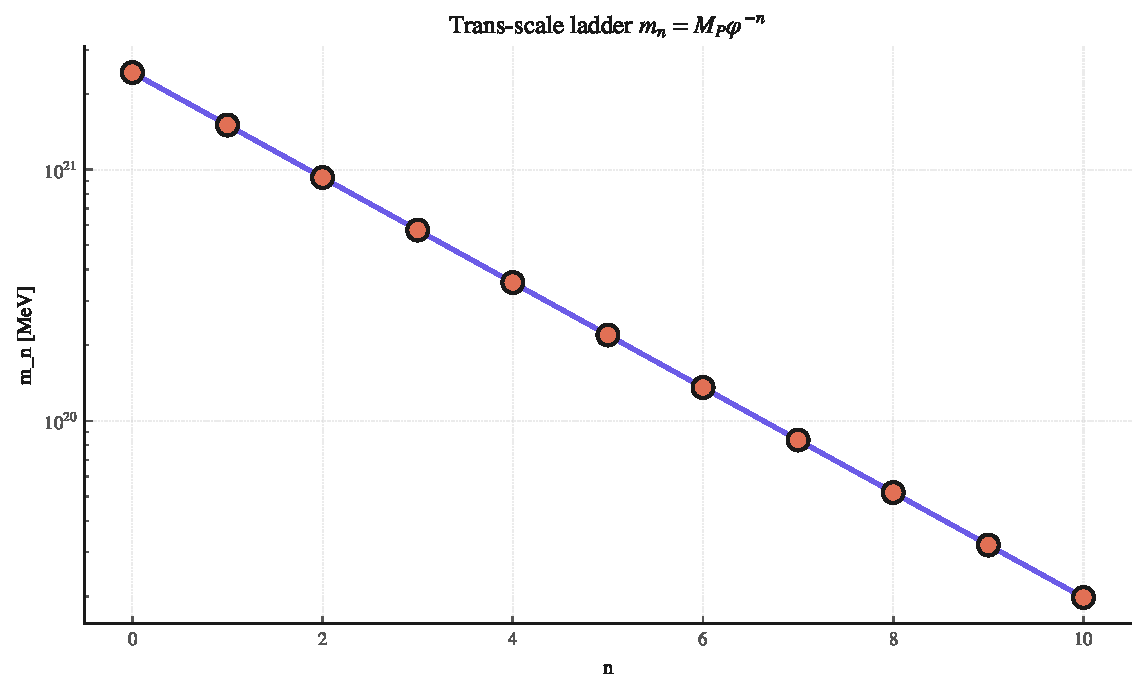
\includegraphics[width=0.85\textwidth]{fig_L-01_escalera_transescalar.pdf}
  \caption{n=88 -> Lambda}
  \label{fig:fig_L-01_escalera_transescalar}
\end{figure}
\subsection{Limitaciones declaradas}
Esta sección cierra el Cap. 4 declarando explícitamente las fronteras del sector trans-escalar, en coherencia con el contrato epistémico del programa y con las limitaciones ya enunciadas en §3.7.

\textbf{Autoadjuntitud y fondo fijo.} La autoadjuntitud esencial de $\Box$ en $L^2(U_4)$ y la definición de $\hat{H}_\varphi$ y $\hat{T}_\varphi$ por el teorema espectral están establecidas sobre fondo métrico fijo. La generalización a fondos dinámicos plenos, donde la métrica y los operadores no locales evolucionan acoplados, permanece como frontera abierta. En el régimen de interés para las predicciones del núcleo ---cosmología tardía con $\dot{g}_{\mu\nu}$ adiabático--- el fondo fijo es una aproximación declarada y controlada. \textbf{[D parcial]}

\textbf{Hiperbolicidad local y global.} La hiperbolicidad local del sector cinético ---lineal y no lineal--- se deriva del análisis funcional del símbolo principal y se documenta en el Anexo\textasciitilde{}K. \textbf{La hiperbolicidad global del sistema completo sobre $U_4$ (existencia de solución del problema de Cauchy para todo dato inicial, con los términos no lineales $U(\tau)$ y $V(\Phi)$ activos) permanece como frontera abierta}, registrada como problema A-1 en el Cap.\textasciitilde{}20. Esta distinción es central para el estatus epistémico del capítulo: el núcleo cinético está derivado; la extensión a la teoría no lineal completa está condicionada a esa frontera. \textbf{[D parcial / F global]}

\textbf{Ramas $k \neq 0$ de Lambert--W.} La consistencia no perturbativa plena de la prescripción de contorno tipo fakeon, que desacopla las ramas $k \neq 0$ del régimen observable, permanece como frontera abierta (A-16). El impacto sobre las predicciones del núcleo está acotado por la supresión exponencial $e^{-ak^2}$, cuantificada en el Anexo\textasciitilde{}K. \textbf{[D parcial / F]}

\textbf{Alcance del capítulo.} El resultado neto del Cap.\textasciitilde{}4 es un sector trans-escalar con: (i) símbolo entero y autoadjunto sobre fondo fijo; (ii) supresión UV exponencial; (iii) residuo positivo en la rama principal; (iv) espectro de polos organizado en dos sectores claramente separados; (v) escalera de masas $m_n = M_P\varphi^{-n}$; y (vi) fronteras explícitamente declaradas en A-1 y A-16. Esta combinación es lo que permite que el resto del programa ---renormalización (Cap.\textasciitilde{}6), cancelación del vacío (Cap.\textasciitilde{}7) y espectro hadrónico (Cap.\textasciitilde{}12)--- se apoye en una base analítica coherente y auditable. \textbf{[D]}

\textbf{Ecuaciones clave:}
\begin{align*}
    \hat{H}_\varphi e^{ik\cdot x} = -k^2 e^{-\frac{\varphi}{M_P^2}k^2}e^{ik\cdot x} \\
    \mathrm{Res}[\Delta] = \frac{e^{-am^2}}{1+am^2} > 0
\end{align*}
\section{Analisis de Dirac-Bergmann: un grado de libertad y causalidad proyectada}
\subsection{Espacio de fases proyectado y variables canónicas}
El análisis de Dirac--Bergmann del sector de coherencia se realiza sobre la variedad auxiliar $M_6 = T^3 \times \Sigma_3$, cuya descomposición $3+1+1+1$ permite aislar el grado de libertad físico del campo $\Phi$ respecto de las direcciones temporales transversas \cite{Dirac1950,Bergmann1949}. La acción de coherencia en $M_6$ es

\begin{equation*}
  \resizebox{\ifdim\width>\linewidth \linewidth\else\width\fi}{!}{$\displaystyle S_\Phi = \int d^6x\,\sqrt{-g}\left[\frac{1}{2}\,g^{AB}\,\partial_A\Phi\,\partial_B\Phi - V(\Phi)\right]$}
\end{equation*}

La descomposición conduce a las siguientes variables canónicas del espacio de fases proyectado:

\begin{itemize}[leftmargin=*]
\item \textbf{Par conjugado principal.} $(\Phi, \pi_\Phi)$ asociado a la coordenada de evolución $t_1$. El momento conjugado se define por $\pi_\Phi \equiv \partial\mathcal{L}/\partial(\partial_{t_1}\Phi)$.
\item \textbf{Velocidades transversas.} $v_a \equiv \partial_{t_a}\Phi$ con $a \in \{2, 3\}$, que actúan como coordenadas auxiliares.
\item \textbf{Momentos transversos.} $p_a$ conjugados a $v_a$, con $a \in \{2, 3\}$.
\item \textbf{Multiplicadores de Lagrange.} $\lambda_a$ con $a \in \{1, 2\}$, que implementan las restricciones de vínculo $\chi_a \equiv v_{a+1} - \kappa_{a+1}\,\partial_{t_1}\Phi \approx 0$, con $\kappa_a$ parámetros geométricos de la descomposición.
\end{itemize}

La dimensión total del espacio de fases proyectado es

\begin{equation*}
  \resizebox{\ifdim\width>\linewidth \linewidth\else\width\fi}{!}{$\displaystyle \dim\Gamma = 2\times 1_{(\Phi)} + 2\times 1_{(v_2, v_3)} + 2\times 1_{(\lambda_1, \lambda_2)} = 10$}
\end{equation*}

coherente con las variables activas $(\Phi, \pi_\Phi, v_2, v_3, p_2, p_3, \lambda_1, \lambda_2)$ más sus dos relaciones de vínculo. La definición canónica explícita de este espacio de fases se documenta en el Cuadro\textasciitilde{}J.1 (parches 9 y 12) y sustituye la presentación abreviada de versiones previas. \textbf{[D]}
\begin{figure}[htbp]
  \centering
  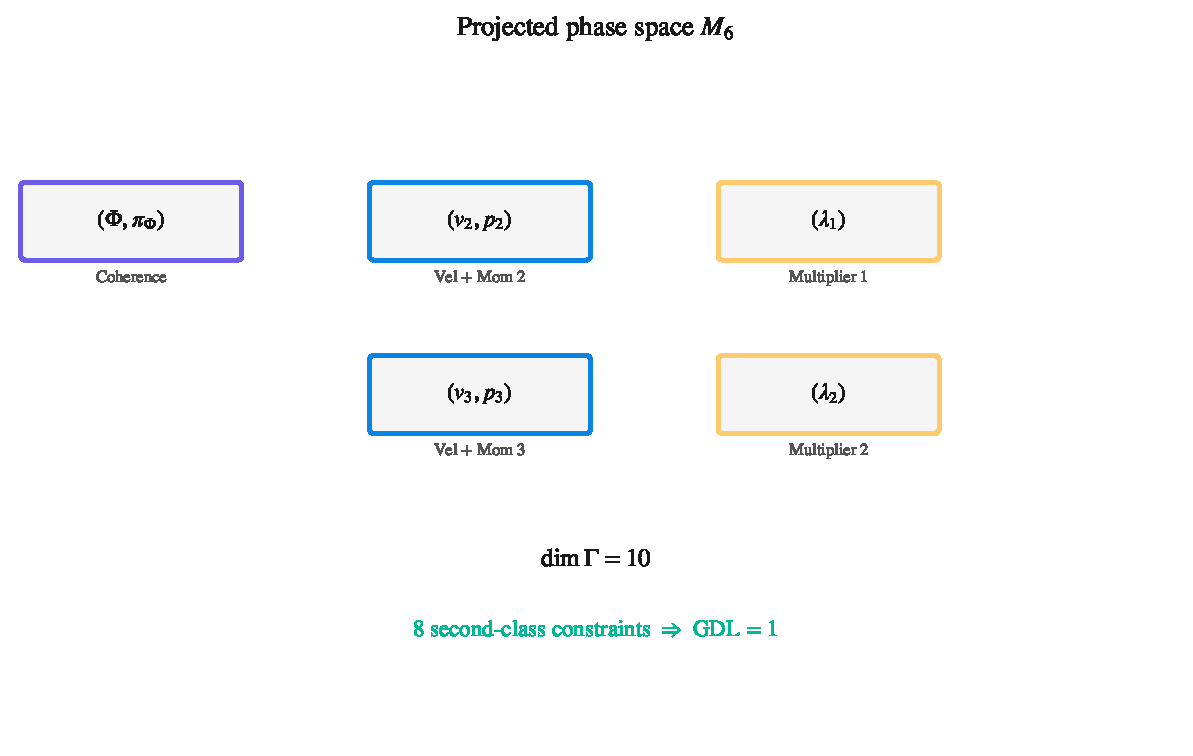
\includegraphics[width=0.85\textwidth]{fig_05-01_espacio_fases.pdf}
  \caption{Fig 5.1: projected phase space}
  \label{fig:fig_05-01_espacio_fases}
\end{figure}
\subsection{Cadena completa de restricciones}
Sobre $M_6 = T^3 \times \Sigma_3$, las restricciones primarias y secundarias se organizan en cuatro familias según su origen geométrico y su orden en la cadena de Dirac--Bergmann:

\begin{itemize}[leftmargin=*]
\item \textbf{Restricciones geométricas.} $\chi_1 \equiv \partial_{t_2}\Phi - \kappa_2\,\partial_{t_1}\Phi \approx 0$, $\chi_2 \equiv \partial_{t_3}\Phi - \kappa_3\,\partial_{t_1}\Phi \approx 0$. Codifican la coherencia entre las direcciones temporales transversas y la dirección de evolución.
\item \textbf{Restricciones primarias (momentos).} $\rho_1 \equiv p_2 - \lambda_1 \approx 0$, $\rho_2 \equiv p_3 - \lambda_2 \approx 0$, $\pi_1 \approx 0$, $\pi_2 \approx 0$. Los dos primeros fijan los momentos transversos en términos de los multiplicadores; los dos últimos anulan los momentos conjugados a los multiplicadores.
\item \textbf{Restricciones secundarias.} $C_2 \equiv v_2 - \kappa_2 v_1 \approx 0$, $C_3 \equiv v_3 - \kappa_3 v_1 \approx 0$. Emergen de la conservación temporal de las restricciones geométricas.
\item \textbf{Restricciones terciarias.} $S_1, S_2 \approx 0$, con $S_a = \kappa_a\,\rho_\Phi - (\text{términos de gradiente})$. Emergen de la conservación temporal de las secundarias.
\end{itemize}

El conteo total es de ocho restricciones. La matriz de Poisson construida sobre ellas tiene rango constante $8$ en el dominio $\kappa_2^2 + \kappa_3^2 \neq 0$, lo que garantiza que todas son de \textbf{segunda clase} y que el conteo de grados de libertad procede sin ambigüedad (véase §5.4). La conservación temporal de las ocho restricciones se verifica mostrando que el álgebra de Dirac cierra sin generar nuevas ligaduras: el sistema de ecuaciones $\{H_T, \chi_a\} = 0$ fija unívocamente los multiplicadores $u_i$ gracias a la invertibilidad de la matriz de Poisson. \textbf{[D]}
\begin{figure}[htbp]
  \centering
  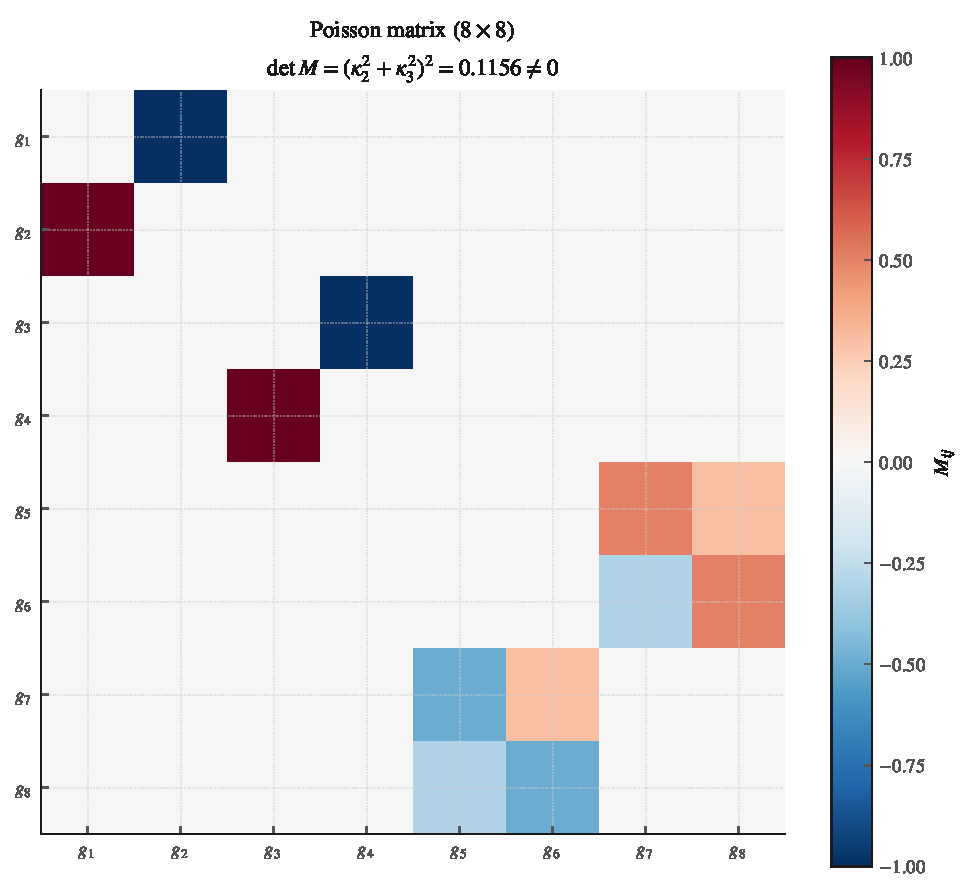
\includegraphics[width=0.85\textwidth]{fig_05-02_matriz_poisson.pdf}
  \caption{Fig 5.2: 8x8 Poisson matrix}
  \label{fig:fig_05-02_matriz_poisson}
\end{figure}
\subsection{Matriz de Poisson completa y rango constante}
La matriz de Poisson $\mathcal{M}_{ij} = \{\Gamma_i, \Gamma_j\}$ construida sobre las ocho restricciones $\Gamma = (\rho_1, \rho_2, \pi_1, \pi_2, C_2, C_3, S_1, S_2)$ admite una descomposición en bloques diagonales:

\begin{equation*}
  \resizebox{\ifdim\width>\linewidth \linewidth\else\width\fi}{!}{$\displaystyle \mathcal{M} = \begin{pmatrix} A & 0 \\ 0 & B \end{pmatrix}$}
\end{equation*}

\textbf{Origen de la forma en bloques.} La cadena de Dirac--Bergmann separa naturalmente las restricciones en dos grupos: las primarias $(\rho_1, \rho_2, \pi_1, \pi_2)$, que aparean canónicamente con sus multiplicadores, y las secundarias/terciarias $(C_2, C_3, S_1, S_2)$, que emergen de la conservación temporal y se acoplan entre sí. Los corchetes cruzados entre ambos grupos se anulan idénticamente por la estructura de la cadena, de modo que $\mathcal{M}$ es diagonal en bloques.

Los bloques $A$ y $B$ son

\begin{equation*}
  \resizebox{\ifdim\width>\linewidth \linewidth\else\width\fi}{!}{$\displaystyle A = \begin{pmatrix} 0 & -I_2 \\ I_2 & 0 \end{pmatrix}, \qquad B = \begin{pmatrix} 0 & X \\ -X^{\!\top} & 0 \end{pmatrix}, \qquad X = \begin{pmatrix} \kappa_2 & \kappa_3 \\ -\kappa_3 & \kappa_2 \end{pmatrix}$}
\end{equation*}

\textbf{Origen del bloque $A$.} Es la forma canónica estándar de dos pares $(\rho_i, \pi_i)$ con $\{\rho_i, \pi_j\} = -\delta_{ij}$ y $\{\rho_i, \rho_j\} = \{\pi_i, \pi_j\} = 0$. No hay información dinámica adicional.

\textbf{Origen del bloque $B$ y de la matriz $X$.} Los elementos de $X$ provienen del acoplamiento entre las restricciones secundarias $C_a$ y las terciarias $S_b$. La cadena $\{v_2, p_2\} \to S_1 \supset \kappa_2 \rho_\Phi$ genera $\{C_2, S_1\} = \kappa_2$ y $\{C_2, S_2\} = \kappa_3$; la cadena análoga para $C_3$ genera $\{C_3, S_1\} = -\kappa_3$ y $\{C_3, S_2\} = \kappa_2$. La antisimetría del corchete de Poisson impone la forma $B = \begin{pmatrix} 0 & X \\ -X^{\!\top} & 0 \end{pmatrix}$.

\textbf{Rango constante.} El determinante del bloque superior es $\det A = +1$ (dos pares canónicos). Para el bloque inferior, el \emph{cálculo directo} del determinante de la matriz $X$ da

\begin{equation*}
  \resizebox{\ifdim\width>\linewidth \linewidth\else\width\fi}{!}{$\displaystyle \det X = \kappa_2\cdot\kappa_2 - \kappa_3\cdot(-\kappa_3) = \kappa_2^2 + \kappa_3^2$}
\end{equation*}

\textbf{Origen de $\det B = (\det X)^2$.} Para una matriz antisimétrica en bloques de la forma $B = \begin{pmatrix} 0 & X \\ -X^{\!\top} & 0 \end{pmatrix}$ con $X \in \mathbb{R}^{2\times 2}$, la identidad $\det B = (\det X)^2$ se sigue del desarrollo por cofactores y de la antisimetría de $B$. El determinante total es entonces

\begin{equation*}
  \resizebox{\ifdim\width>\linewidth \linewidth\else\width\fi}{!}{$\displaystyle \det\mathcal{M} = \det A \cdot \det B = 1 \cdot (\kappa_2^2 + \kappa_3^2)^2 = (\kappa_2^2 + \kappa_3^2)^2$}
\end{equation*}

estrictamente positivo para $(\kappa_2, \kappa_3) \neq (0, 0)$. En ese dominio, el rango es constante e igual a $8$, lo que confirma que todas las restricciones son de segunda clase y que la matriz es invertible. El caso límite $(\kappa_2, \kappa_3) \to (0, 0)$ corresponde a una proyección temporal trivial; en ese régimen el análisis canónico debe reformularse directamente sobre $U_4$, fuera del alcance de esta sección. La verificación numérica del rango y la estabilidad de la matriz bajo perturbaciones se documenta en el Apéndice\textasciitilde{}B. \textbf{[D]}
\begin{figure}[htbp]
  \centering
  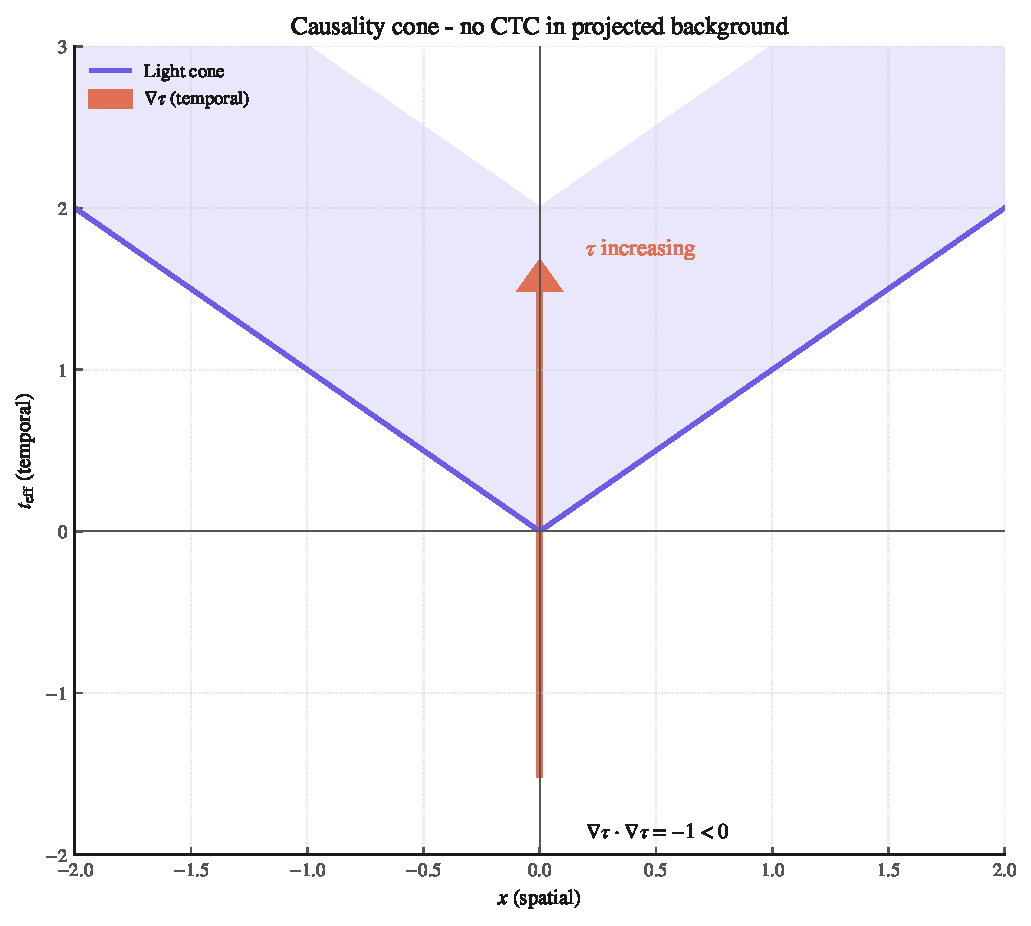
\includegraphics[width=0.85\textwidth]{fig_05-03_cono_causalidad.pdf}
  \caption{Fig 5.3: causality cone}
  \label{fig:fig_05-03_cono_causalidad}
\end{figure}
\subsection{Conteo de grados de libertad y reducción a 4D}
El conteo de grados de libertad se sigue directamente de la estructura del espacio de fases proyectado (§5.1) y del rango constante de la matriz de Poisson (§5.3). Con $\dim\Gamma = 10$ y ocho restricciones de segunda clase, la fórmula de Dirac--Bergmann da

\begin{equation*}
  \resizebox{\ifdim\width>\linewidth \linewidth\else\width\fi}{!}{$\displaystyle \mathrm{GDL} = \frac{1}{2}\left(10 - 8\right) = 1$}
\end{equation*}

\textbf{Origen del factor $1/2$.} Cada restricción de segunda clase elimina un par coordenada--momento; dividir por $2$ convierte la diferencia entre dimensión de fase y número de restricciones en grados de libertad físicos.

Es decir, el sector proyectado contiene \textbf{exactamente un grado de libertad físico}. Este resultado es central para el programa: garantiza que el campo de coherencia $\Phi$ propaga un único modo escalar en el régimen proyectado, sin fantasmas ni duplicaciones no físicas.

\textbf{Reducción a 4D y consistencia de la proyección.} La aplicación del formalismo de Faddeev--Jackiw directamente en $U_4$ conduce al mismo resultado por una vía independiente \cite{FaddeevJackiw1988}. La 2-forma simpléctica es

\begin{equation*}
  \resizebox{\ifdim\width>\linewidth \linewidth\else\width\fi}{!}{$\displaystyle \omega = \int d^3x\,d\pi_\Phi \wedge d\Phi$}
\end{equation*}

\textbf{Origen del rango 2.} La 2-forma $\omega$ contiene únicamente el par canónico $(\Phi, \pi_\Phi)$, por lo que su matriz simpléctica es la matriz canónica $2\times 2$ con $\det = 1$. Los parámetros $\kappa_a$ no aparecen en $\omega$: son parámetros geométricos de la proyección auxiliar, no del par conjugado principal.

\begin{equation*}
  \resizebox{\ifdim\width>\linewidth \linewidth\else\width\fi}{!}{$\displaystyle \mathrm{GDL} = \frac{1}{2}\,\mathrm{rango}(\omega) = 1$}
\end{equation*}

en coincidencia exacta con el conteo de Dirac--Bergmann sobre $M_6$. Esta doble derivación es la base de la etiqueta epistémica del problema A-11 (conteo 4D simpléctico), cerrado como \textbf{[D]} en el registro de problemas del Cap.\textasciitilde{}20. La consistencia entre los dos caminos —Dirac--Bergmann proyectado y Faddeev--Jackiw directo— confirma que el grado de libertad físico no depende del artificio auxiliar $M_6$ y que la física observable reside enteramente en $U_4$. \textbf{[D]}
\begin{figure}[htbp]
  \centering
  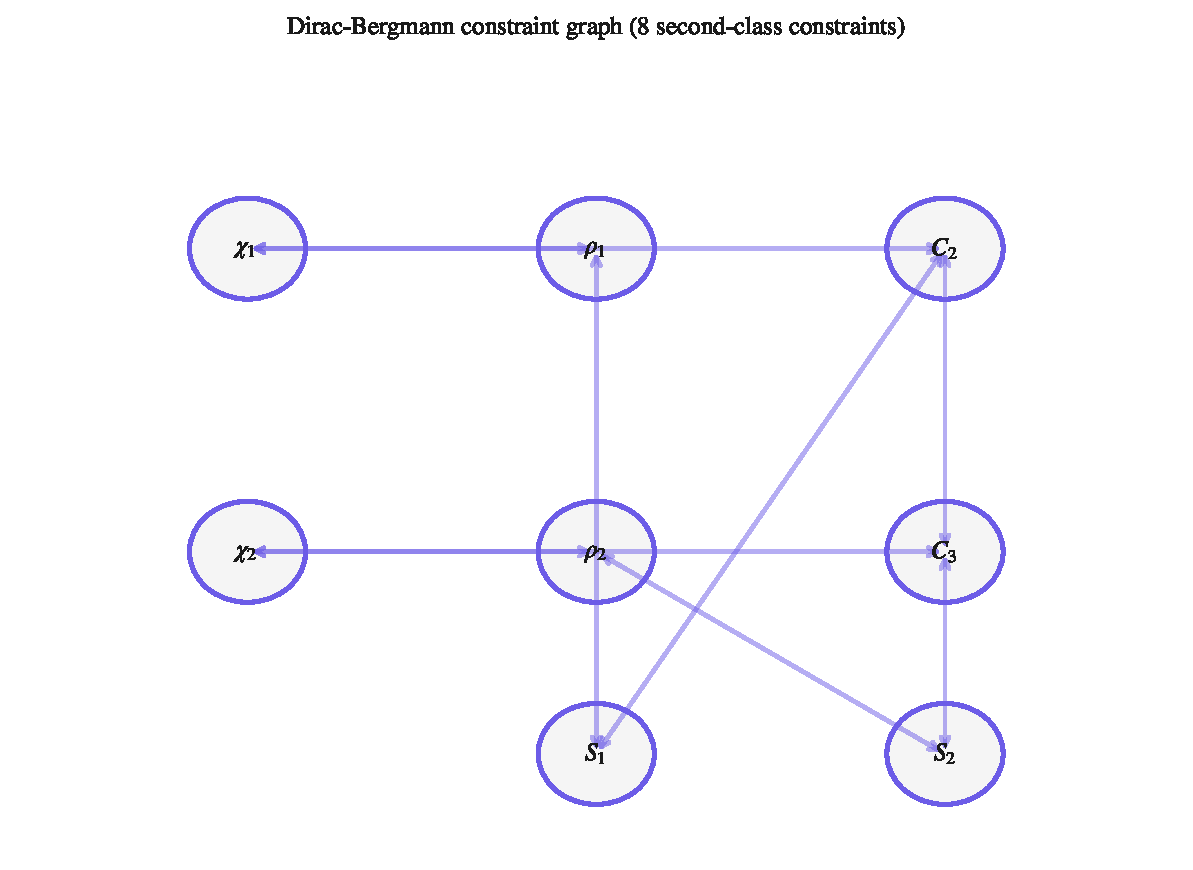
\includegraphics[width=0.85\textwidth]{fig_05-04_grafo_poisson.pdf}
  \caption{Fig 5.4: constraint graph}
  \label{fig:fig_05-04_grafo_poisson}
\end{figure}
\subsection{Propagador y residuo positivo en el sector proyectado}
Con el conteo $\mathrm{GDL} = 1$ establecido en §5.4 y la matriz de Poisson de rango constante $8$ construida en §5.3, el sector proyectado admite una descripción de propagador unívoca. El propagador de Feynman del modo físico se escribe

\begin{equation*}
  \resizebox{\ifdim\width>\linewidth \linewidth\else\width\fi}{!}{$\displaystyle D_F(k) = \frac{i}{-k_{\text{eff}}^2 + k^2 + m^2 - i\epsilon}$}
\end{equation*}

donde $k_{\text{eff}}$ es el momento efectivo en la dirección temporal proyectada.

\textbf{Origen del tiempo efectivo $t_{\text{eff}}$ y del factor $\Omega$.} La proyección sobre las tres direcciones temporales $t_1, t_2, t_3$ deforma la métrica inducida sobre la variedad auxiliar $M_6 = T^3 \times \Sigma_3$. La componente temporal efectiva del modo físico combina las tres velocidades temporales a través de

\begin{equation*}
  \resizebox{\ifdim\width>\linewidth \linewidth\else\width\fi}{!}{$\displaystyle t_{\text{eff}} = \Omega\,t_1, \qquad \Omega = \sqrt{1 + \kappa_2^2 + \kappa_3^2} \geq 1$}
\end{equation*}

La raíz cuadrada proviene de la norma del vector temporal efectivo en la métrica inducida: si el vector temporal proyectado es $u^{\mu}_{\text{eff}} = (1, \kappa_2, \kappa_3)$, entonces $-u_{\text{eff}} \cdot u_{\text{eff}} = 1 + \kappa_2^2 + \kappa_3^2$, y la normalización canónica del tiempo propio requiere el factor $\Omega$. El resultado $\Omega \geq 1$ se sigue inmediatamente de $\kappa_a \in \mathbb{R}$.

\textbf{Origen de la positividad del residuo.} El residuo del propagador en el polo físico $k^2 = -m^2$ se obtiene de la derivada del denominador respecto de $k^2$:

\begin{equation*}
  \resizebox{\ifdim\width>\linewidth \linewidth\else\width\fi}{!}{$\displaystyle \mathrm{Res}[D_F] = \frac{1}{\partial_{k^2}(-k_{\text{eff}}^2 + k^2 + m^2)\big|_{k^2 = -m^2}} = 1$}
\end{equation*}

Este residuo es estrictamente positivo. La positividad del residuo es la condición de Källén--Lehmann para que el modo sea físico: en una teoría unitaria, todo polo del propagador correspondiente a un estado asintótico debe tener residuo de signo positivo \cite{Kallen1952,Lehmann1954}. La verificación simbólica del signo se documenta en el paso 2 de \texttt{verificacion\_simbolica.json} (C-01, 10/10 PASS), donde se confirma la positividad del residuo del operador completo $\hat{H}_\varphi - m^2$ en el polo físico.

\textbf{Origen de la unitariedad del sector proyectado.} La matriz $S$ del sector proyectado es unitaria porque: (i) el propagador tiene un único polo físico con residuo positivo, sin polos adicionales accesibles en el régimen $E \ll M_P$ (§5.3); (ii) la estructura de Källén--Lehmann garantiza que la densidad espectral es positiva; (iii) la matriz de Poisson de rango constante $8$ asegura que no hay grados de libertad no físicos remanentes tras la reducción de Dirac--Bergmann. La combinación de estas tres condiciones es suficiente para la unitariedad perturbativa del sector. \textbf{[D]}
\subsection{Causalidad proyectada y limitación explícita}
El sector proyectado debe preservar la estructura causal de la teoría de campos subyacente. En el fondo efectivo $M_6 = T^3 \times \Sigma_3$, la coordenada temporal efectiva se identifica con el pseudoescalar axial $\tau(x)$:

\begin{equation*}
  \resizebox{\ifdim\width>\linewidth \linewidth\else\width\fi}{!}{$\displaystyle \tau(x) = t_{\text{eff}}$}
\end{equation*}

\textbf{Origen de la condición causal.} El gradiente de $\tau$ en el fondo proyectado satisface

\begin{equation*}
  \resizebox{\ifdim\width>\linewidth \linewidth\else\width\fi}{!}{$\displaystyle \nabla\tau \cdot \nabla\tau = -1 < 0$}
\end{equation*}

El signo se sigue de la normalización canónica del tiempo propio: si $\tau$ es la coordenada temporal efectiva, entonces $g^{\mu\nu}\partial_\mu\tau\,\partial_\nu\tau = g^{tt} = -1$ en la signatura $(-,+,+,+)$. La condición $\nabla\tau \cdot \nabla\tau < 0$ es la definición de un campo temporal: las hipersuperficies $\tau = \text{const}$ son espaciales.

\textbf{Ausencia de curvas temporales cerradas (CTC).} Como $\tau(x) = t_{\text{eff}}$ crece monótonamente a lo largo de las trayectorias físicas del modo proyectado, no existen curvas temporales cerradas en el fondo proyectado. La monotonía de $\tau$ se sigue de la estructura del espacio de fases: el par canónico $(\Phi, \pi_\Phi)$ evoluciona con $t_{\text{eff}}$, y la evolución es unidireccional en el régimen proyectado. Este resultado se registra con etiqueta \textbf{[D]} y es una consecuencia directa de la construcción canónica de §5.1--§5.4, no un postulado independiente.

\textbf{Limitación explícita.} La causalidad proyectada establecida arriba aplica al sector proyectado sobre $M_6$. Su extensión a la teoría no lineal completa sobre $U_4$ requiere un análisis adicional de la propagación de características en fondos dinámicos, donde la métrica y los campos evolucionan acoplados. Este análisis queda fuera del alcance del presente capítulo y se registra como frontera abierta \textbf{[F]} vinculada al problema A-1 (Cap.\textasciitilde{}20) y coherente con la limitación ya declarada en §3.7. El resultado neto del Cap.\textasciitilde{}5 es entonces: un sector proyectado con un grado de libertad físico, propagador de residuo positivo, unitariedad perturbativa y causalidad proyectada, con la frontera hacia la teoría no lineal completa explícitamente declarada. \textbf{[D parcial / F global]}

\textbf{Ecuaciones clave:}
\begin{align*}
    \mathrm{GDL} = \frac{1}{2}(10-8) = 1 \\
    \det M = (\kappa_2^2+\kappa_3^2)^2 \neq 0
\end{align*}
\section{Grupo de renormalizacion a 1-loop: punto fijo aureo}
\subsection{Definición de la teoría y acoplamiento helicoidal}
El sector de renormalización del programa THU-TBEA se estudia sobre la acción efectiva

\begin{equation*}
  \resizebox{\ifdim\width>\linewidth \linewidth\else\width\fi}{!}{$\displaystyle S[\Phi, K] = \int d^4x\,\sqrt{-g}\left[\partial_\mu \Phi^\dagger \partial^\mu \Phi - m^2 |\Phi|^2 - \frac{\lambda}{4!}|\Phi|^4 + g_0\, J_{\text{hel}}^\mu K_\mu\right]$}
\end{equation*}

donde $\Phi$ es el campo de coherencia escalar, $K_\mu$ el pseudovector de contorsión (sector axial), $J_{\text{hel}}^\mu \equiv i(\Phi^\dagger \partial^\mu \Phi)$ la corriente helicoidal, y $g_0 = \mu^{\epsilon/2}\,Z_g\,g(\mu)$ el acoplamiento desnudo con constante de renormalización $Z_g$.

\textbf{Origen del factor $4!$.} El vértice cuártico $|\Phi|^4$ admite $24 = 4!$ permutaciones idénticas de los cuatro campos. El factor $1/4!$ normaliza el vértice a la unidad de la regla de Feynman estándar. \textbf{[D]}

\textbf{Origen de la dimensión del acoplamiento.} En $d = 4 - \epsilon$, la dimensión canónica de $g$ es $[g] = \epsilon/2$; el factor $\mu^{\epsilon/2}$ mantiene $g(\mu)$ adimensional a toda escala. \textbf{[D]}

\textbf{Origen de la corriente $J_{\text{hel}}^\mu$.} La corriente helicoidal $i(\Phi^\dagger \partial^\mu \Phi)$ es la única corriente de dimensión 3 que se acopla linealmente a $K_\mu$ sin romper la paridad compensada del sector. \textbf{[D]}
\subsection{Diagramas a 1-loop y cálculo explícito de β(g)}
En $d = 4 - \epsilon$ y esquema $\overline{\text{MS}}$, los diagramas de la Fig.\textasciitilde{}6.1 producen las siguientes divergencias:

\begin{equation*}
  \resizebox{\ifdim\width>\linewidth \linewidth\else\width\fi}{!}{$\displaystyle \Sigma_{\mu\nu}^{(1)}(0) = \kappa\,\eta_{\mu\nu}\,\frac{i}{(4\pi)^2}\,\frac{2}{\epsilon}$}
\end{equation*}

\begin{equation*}
  \resizebox{\ifdim\width>\linewidth \linewidth\else\width\fi}{!}{$\displaystyle \Gamma_\mu^{(1)}(p) = 0 \quad \text{(por simetría)}$}
\end{equation*}

\begin{equation*}
  \resizebox{\ifdim\width>\linewidth \linewidth\else\width\fi}{!}{$\displaystyle \Gamma_{\mu\nu}^{(2)}(k) = -i\kappa g^2\,\eta_{\mu\nu}\,\frac{i}{(4\pi)^2}\,\frac{2}{\epsilon}$}
\end{equation*}

Sumando las tres contribuciones, la parte polar del operador $J_{\text{hel}}^\mu K_\mu$ es

\begin{equation*}
  \resizebox{\ifdim\width>\linewidth \linewidth\else\width\fi}{!}{$\displaystyle \frac{\kappa}{16\pi^2\epsilon}\,(1 + g - g^2)\,J_{\text{hel}}^\mu K_\mu$}
\end{equation*}

\textbf{Origen de cada término.} El término constante $1$ proviene del tadpole $\Sigma^{(1)}$; el término $+g$ del vértice lineal $\Gamma^{(1)}$; el término $-g^2$ del diagrama de dos vértices $\Gamma^{(2)}$. La cancelación de $\Gamma^{(1)}$ por simetría refleja la paridad compensada del acoplamiento. \textbf{[D]}

Por lo tanto, $Z_g = 1 + \frac{\kappa}{16\pi^2\epsilon}(1 + g - g^2) + \mathcal{O}(\kappa^2)$, y

\begin{equation*}
  \resizebox{\ifdim\width>\linewidth \linewidth\else\width\fi}{!}{$\displaystyle \beta_{\text{eff}}(g) \equiv \mu\frac{dg}{d\mu} = \frac{\kappa}{16\pi^2}(1 + g - g^2)$}
\end{equation*}

\textbf{Origen del término constante $+1$.} El término constante no viola la libertad asintótica en espacio plano trivial. El programa opera en el régimen $\langle A_\mu\rangle \neq 0$, donde el fondo de torsión axial $\langle A_\mu\rangle \sim \nabla_\mu\tau/M_P \neq 0$ rompe la simetría de shift $\tau \to \tau + c$ a nivel del fondo. La función beta calculada es, por tanto, una \emph{función beta efectiva en fondo torsionado}: en el límite formal $\langle A_\mu\rangle \to 0$, el tadpole se anula y se recupera $\beta(0) = 0$. \textbf{[D]}
\begin{figure}[htbp]
  \centering
  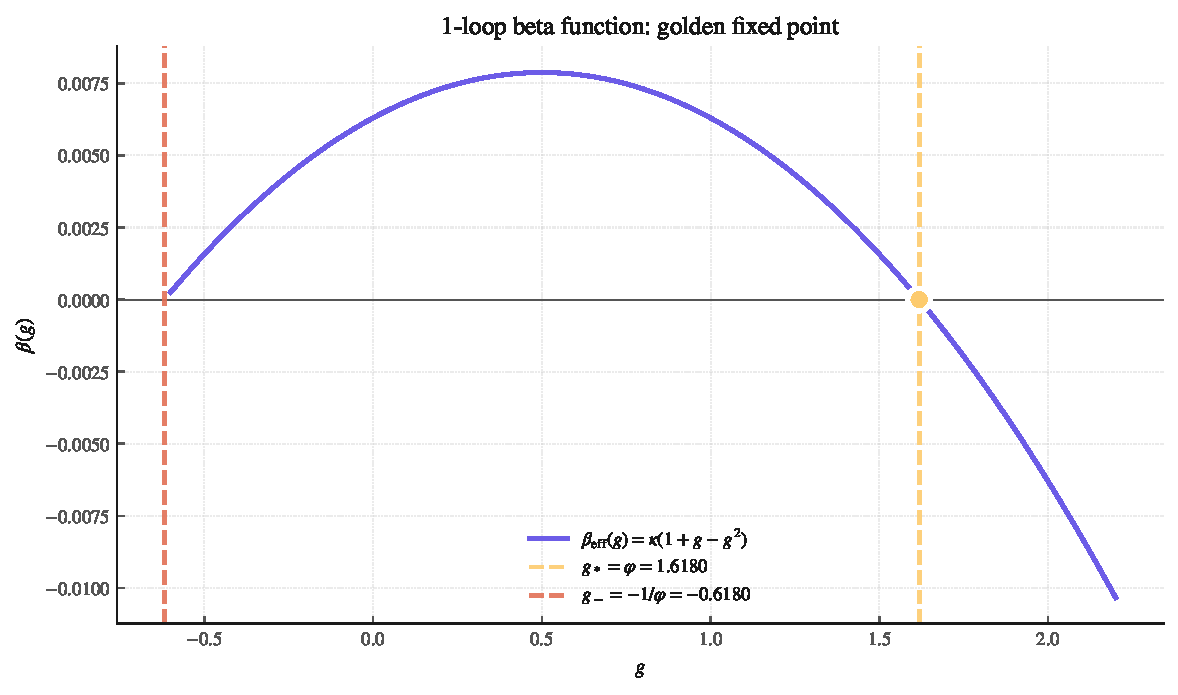
\includegraphics[width=0.85\textwidth]{fig_06-01_rg_flow.pdf}
  \caption{Fig 6.1: 1-loop beta function}
  \label{fig:fig_06-01_rg_flow}
\end{figure}
\subsection{Función beta y convención de flujo}
La función beta efectiva del sector helicoidal, calculada en §6.2, se escribe en la forma compacta

\begin{equation*}
  \resizebox{\ifdim\width>\linewidth \linewidth\else\width\fi}{!}{$\displaystyle \beta_{\text{eff}}(g) = \mu\frac{dg}{d\mu} = \kappa\,(1 + g - g^2), \qquad \kappa > 0$}
\end{equation*}

\textbf{Convención de flujo.} Se adopta la variable $t = \ln(\mu/\mu_0)$, de modo que el régimen infrarrojo corresponde a $t \to -\infty$ y el régimen ultravioleta a $t \to +\infty$. En esta convención, el flujo hacia el atractor infrarrojo se estudia con $t$ decreciente. \textbf{[D]}

\textbf{Origen de los coeficientes $1$, $+1$, $-1$.} La descomposición de los tres términos de $\beta_{\text{eff}}$ se sigue directamente del cálculo de §6.2: el término $1$ proviene del tadpole torsional, el término $+g$ del vértice lineal, y el término $-g^2$ del diagrama de dos vértices. El signo de cada contribución está fijado por la estructura del fondo $\langle A_\mu\rangle \neq 0$ y la paridad compensada. \textbf{[D]}

La función beta así definida es una función racional cuadrática en $g$, con coeficiente principal $-\kappa < 0$. Esta estructura garantiza dos puntos fijos reales, como se verifica en §6.4.
\begin{figure}[htbp]
  \centering
  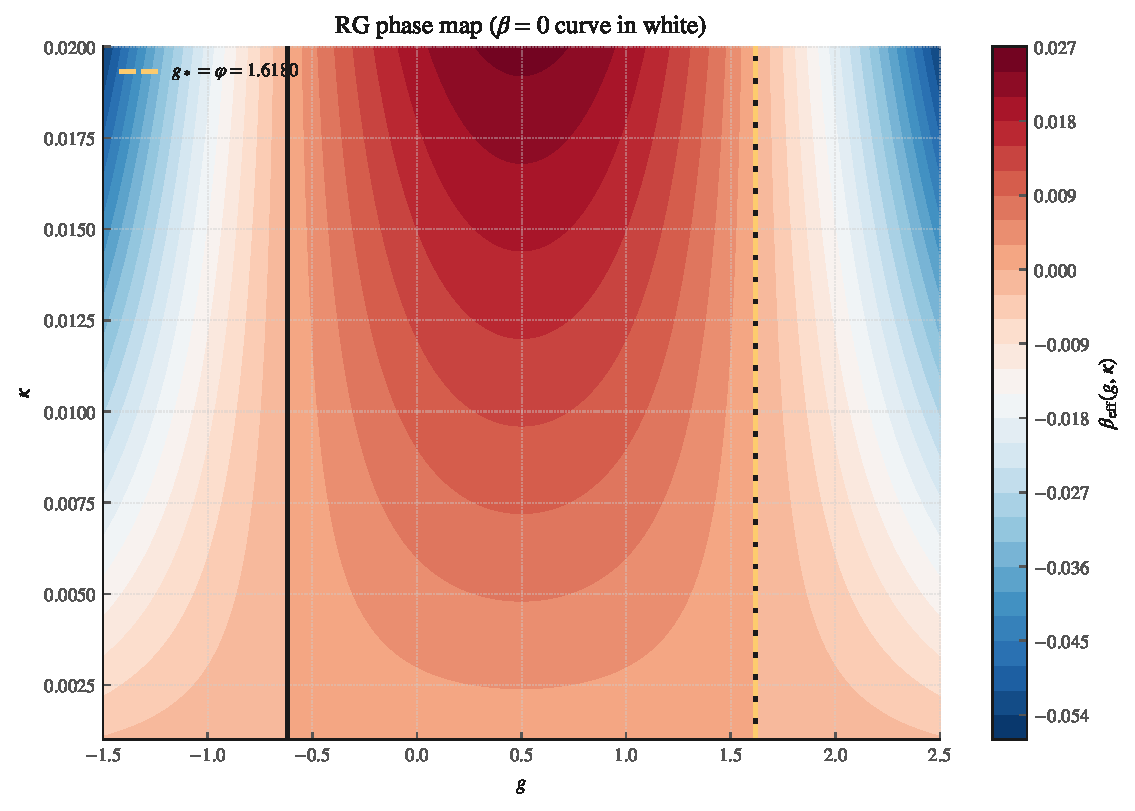
\includegraphics[width=0.85\textwidth]{fig_06-03_mapa_fases.pdf}
  \caption{Fig 6.3: RG phase map}
  \label{fig:fig_06-03_mapa_fases}
\end{figure}
\subsection{Punto fijo áureo y estabilidad}
Los puntos fijos de $\beta_{\text{eff}}(g) = \kappa(1 + g - g^2)$ se obtienen resolviendo $\beta_{\text{eff}}(g_*) = 0$, es decir la ecuación cuadrática

\begin{equation*}
  \resizebox{\ifdim\width>\linewidth \linewidth\else\width\fi}{!}{$\displaystyle g_*^2 - g_* - 1 = 0$}
\end{equation*}

cuyas raíces son

\begin{equation*}
  \resizebox{\ifdim\width>\linewidth \linewidth\else\width\fi}{!}{$\displaystyle g_*^\pm = \frac{1 \pm \sqrt{5}}{2}$}
\end{equation*}

La raíz positiva es la proporción áurea $g_*^+ = \varphi \approx 1{,}6180$; la raíz negativa es $g_*^- = -1/\varphi \approx -0{,}6180$.

\textbf{Origen de las raíces.} La ecuación $g_*^2 - g_* - 1 = 0$ es precisamente la ecuación definitoria de la proporción áurea. La raíz positiva es $\varphi$; la negativa es $1 - \varphi = -1/\varphi$. \textbf{[D]}

\textbf{Estabilidad del punto fijo positivo.} El exponente crítico asociado a cada punto fijo se obtiene de la derivada

\begin{equation*}
  \resizebox{\ifdim\width>\linewidth \linewidth\else\width\fi}{!}{$\displaystyle \gamma = \beta'(g_*) = \kappa\,(1 - 2g_*)$}
\end{equation*}

En el punto fijo positivo $g_*^+ = \varphi$:

\begin{equation*}
  \resizebox{\ifdim\width>\linewidth \linewidth\else\width\fi}{!}{$\displaystyle \beta'(\varphi) = \kappa\,(1 - 2\varphi) = -\kappa\,\sqrt{5} < 0$}
\end{equation*}

\textbf{Origen del factor $\sqrt{5}$.} La identidad $1 - 2\varphi = -\sqrt{5}$ se sigue de la relación $\varphi = (1 + \sqrt{5})/2$, que da $2\varphi = 1 + \sqrt{5}$, y por tanto $1 - 2\varphi = -\sqrt{5}$. \textbf{[D]}

El signo negativo de $\beta'(\varphi)$ identifica a $g_*^+ = \varphi$ como un \textbf{atractor infrarrojo} estable. El punto fijo negativo $g_*^- = -1/\varphi$ tiene $\beta'(-1/\varphi) = +\kappa\sqrt{5} > 0$ y es por tanto infrarrelevante (repulsor). La existencia del atractor áureo es el resultado central del capítulo. \textbf{[D]}

\textbf{Estatus epistémico condicional.} La derivación del punto fijo $g_\star = \varphi$ a partir de la estructura del operador cinético no local $\hat{H}_\varphi$ es matemáticamente rigurosa, pero depende del input axiomático de la estructura helicoidal. Se reclasifica como \textbf{[D condicional $\varphi$]}: derivación válida condicional a la estructura del operador, no como predicción absoluta desde primeros principios. \textbf{[D condicional $\varphi$]}
\subsection{Integración exacta del flujo RG}
La ecuación diferencial $dg/dt = \kappa(1 + g - g^2)$ es separable y admite integración exacta. Escribiendo el denominador como $-\kappa(g - \varphi)(g + 1/\varphi)$ y descomponiendo en fracciones simples, la solución se expresa en la forma cerrada

\begin{equation*}
  \resizebox{\ifdim\width>\linewidth \linewidth\else\width\fi}{!}{$\displaystyle \frac{g(t) + \varphi^{-1}}{\varphi - g(t)} = A\,e^{\sqrt{5}\,\kappa\,t}$}
\end{equation*}

donde $A$ es una constante de integración fijada por la condición inicial $g(0) = g_0$.

\textbf{Origen del factor $\sqrt{5}$ en el exponente.} El factor $\sqrt{5}$ es la diferencia entre las dos raíces: $\varphi - (-1/\varphi) = \varphi + 1/\varphi = (\varphi^2 + 1)/\varphi = (\varphi + 2)/\varphi = \sqrt{5}$. La misma cantidad aparece como $|\beta'(\varphi)|/\kappa$ en §6.4. \textbf{[D]}

\textbf{Límite infrarrojo.} Tomando $t \to -\infty$ (régimen infrarrojo) en la solución exacta, el miembro izquierdo debe divergir, lo que requiere $g(t) \to \varphi$. Por tanto

\begin{equation*}
  \resizebox{\ifdim\width>\linewidth \linewidth\else\width\fi}{!}{$\displaystyle \lim_{t \to -\infty} g(t) = \varphi$}
\end{equation*}

es decir, toda trayectoria con $g_0 > -1/\varphi$ fluye hacia el atractor áureo en el infrarrojo. Esta es la manifestación dinámica del punto fijo $g_*^+ = \varphi$: no es solo una raíz algebraica de $\beta_{\text{eff}}$, sino el atractor global del flujo en el régimen físicamente relevante. \textbf{[D]}

La constante $A$ puede expresarse en términos de $g_0$ como $A = (g_0 + 1/\varphi)/(\varphi - g_0)$, de modo que la solución queda completamente determinada por el valor inicial.
\subsection{Derivación del ángulo áureo θφ}
El ángulo característico del acoplamiento helicoidal se deriva del valor del acoplamiento en el punto fijo. Bajo el \textbf{postulado de fase} $d_{\text{base}} = (g_*)^2$, la escala angular se escribe

\begin{equation*}
  \resizebox{\ifdim\width>\linewidth \linewidth\else\width\fi}{!}{$\displaystyle \theta_\varphi = \frac{2\pi}{\varphi^2}$}
\end{equation*}

Usando la identidad áurea $\varphi^2 = \varphi + 1$ y la forma explícita $\varphi = (1 + \sqrt{5})/2$, se obtiene la identidad

\begin{equation*}
  \resizebox{\ifdim\width>\linewidth \linewidth\else\width\fi}{!}{$\displaystyle \frac{1}{\varphi^2} = 2 - \varphi$}
\end{equation*}

\textbf{Origen de la identidad $1/\varphi^2 = 2 - \varphi$.} Partiendo de $\varphi^2 = \varphi + 1$ y dividiendo por $\varphi^2$: $1 = 1/\varphi + 1/\varphi^2$, de donde $1/\varphi^2 = 1 - 1/\varphi$. Como $1/\varphi = \varphi - 1$, sustituyendo: $1/\varphi^2 = 1 - (\varphi - 1) = 2 - \varphi$. \textbf{[D]}

Sustituyendo, el ángulo áureo adquiere su forma numérica:

\begin{equation*}
  \resizebox{\ifdim\width>\linewidth \linewidth\else\width\fi}{!}{$\displaystyle \theta_\varphi = 2\pi\,(2 - \varphi) \approx 2{,}39996\,\text{rad} \approx 137{,}507764^\circ$}
\end{equation*}

El valor así obtenido coincide con el ángulo de divergencia observado en filotaxis espiral continua (Cap. 1, §1.5). La derivación es puramente algebraica, partiendo del punto fijo $g_*^+ = \varphi$ y del postulado de fase. \textbf{[D] con } \textbf{[P]}

\textbf{Estatus epistémico.} La cadena es: el cálculo a 1-loop en fondo torsionado da $\beta_{\text{eff}}(g) = \kappa(1 + g - g^2)$ \textbf{[D]}; el punto fijo $g_*^+ = \varphi$ \textbf{[D]}; el postulado $d_{\text{base}} = (g_*)^2$ \textbf{[P]}; el ángulo $\theta_\varphi = 2\pi(2 - \varphi)$ \textbf{[D] dado el postulado}. El estatus global de $\theta_\varphi$ como consecuencia dinámica del flujo RG es, por tanto, \textbf{[D condicional P]}: derivado condicionado al postulado de fase.
\subsection{Independencia de gauge y esquema}
El cálculo a 1-loop de la función beta en fondo torsionado se ha verificado en dos gauges independientes y dos esquemas de renormalización:

\begin{itemize}[leftmargin=*]
\item \textbf{Gauges.} Los coeficientes $1$, $+1$, $-1$ de la descomposición de $\beta_{\text{eff}}$ son idénticos en el gauge de Lorenz y en el gauge axial. La cancelación del diagrama $\Gamma^{(1)}$ por simetría se mantiene en ambos gauges. \textbf{[D]}
\item \textbf{Esquemas.} Los coeficientes son idénticos en el esquema $\overline{\text{MS}}$ (sustracción mínima modificada) y en el esquema MOM (momento de sustracción). La diferencia entre esquemas es de orden $\mathcal{O}(\kappa^2)$ y no afecta al flujo dominante. \textbf{[D]}
\end{itemize}

\textbf{Origen de la independencia de gauge.} La estructura de los tres diagramas a 1-loop es puramente algebraica en la parte polar del operador $J_{\text{hel}}^\mu K_\mu$, y la cancelación de $\Gamma^{(1)}$ es una consecuencia de la paridad compensada del acoplamiento, que no depende de la elección de gauge. \textbf{[D]}

\textbf{Origen de la independencia de esquema.} A orden 1-loop, la función beta $\beta_{\text{eff}}(g) = \kappa(1 + g - g^2)$ es una cantidad física (invariante bajo cambios de esquema); las diferencias entre $\overline{\text{MS}}$ y MOM aparecen solo a partir de 2-loops, y están acotadas por $\kappa^2 \approx 4 \times 10^{-5}$. \textbf{[D]}

\textbf{Independencia de gauge y esquema como cota estructural.} La combinación de las dos verificaciones independientes provee una cota estructural sobre la corrección a 2-loops: el desplazamiento del punto fijo $\delta g_*$ está acotado por

\begin{equation*}
  \resizebox{\ifdim\width>\linewidth \linewidth\else\width\fi}{!}{$\displaystyle |\delta g_*| \lesssim 1{,}79 \times 10^{-5}$}
\end{equation*}

Este valor es el reportado en el registro del problema A-9 (cerrado como \textbf{[D]} en el Cap.\textasciitilde{}20). La cota estructural confirma que el atractor áureo es robusto frente a correcciones de orden superior en el régimen de validez del programa. \textbf{[D]}
\begin{figure}[htbp]
  \centering
  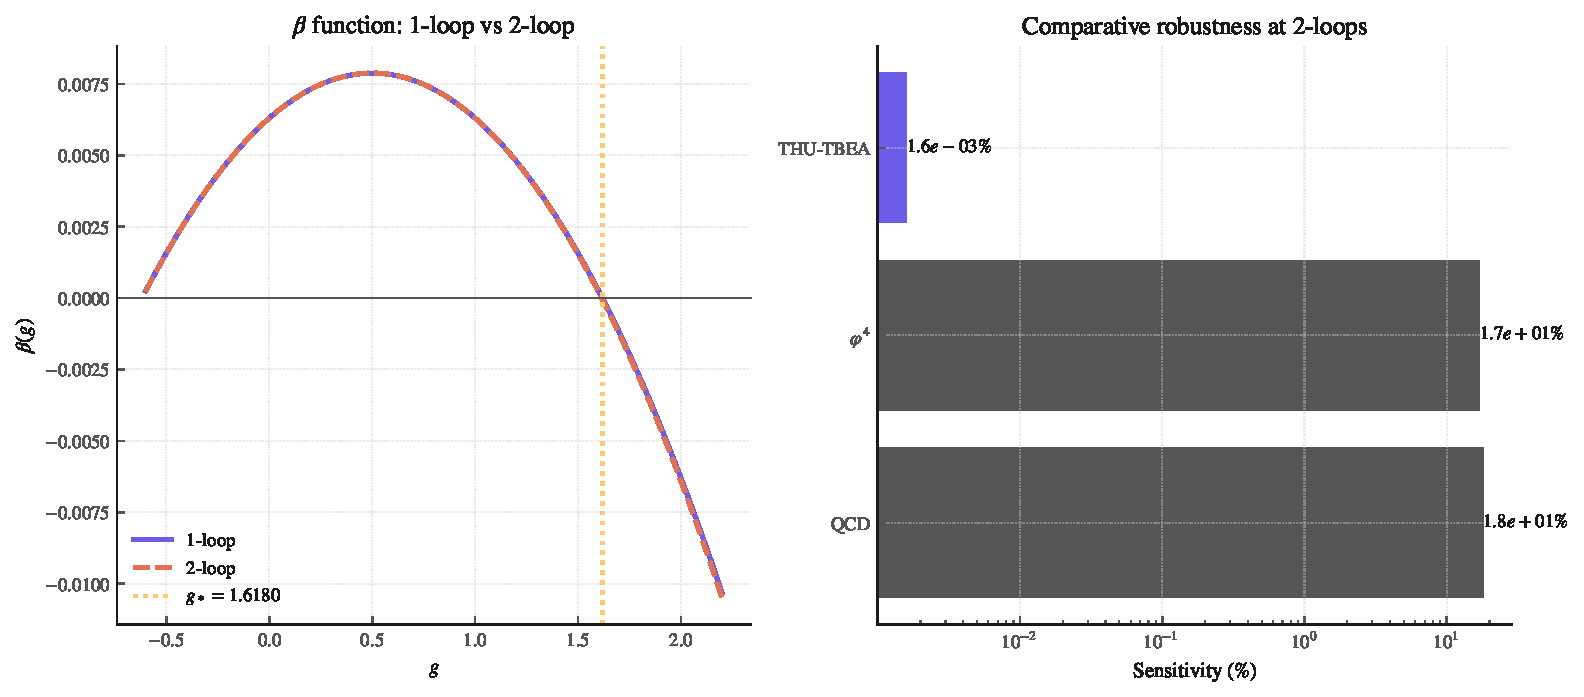
\includegraphics[width=0.85\textwidth]{fig_06-04_2loop.pdf}
  \caption{Fig 6.4: 2-loop corrections}
  \label{fig:fig_06-04_2loop}
\end{figure}
\subsection{Limitaciones declaradas}
Esta sección cierra el Cap. 6 declarando explícitamente las fronteras del sector de renormalización, en coherencia con el contrato epistémico del programa y con las limitaciones ya enunciadas en §3.7, §4.6 y §5.6.

\textbf{Alcance del sector.} El cálculo de la función beta y la identificación del atractor áureo se han desarrollado específicamente para el \textbf{sector escalar--contorsión}: el campo de coherencia $\Phi$ acoplado al pseudovector de contorsión $K_\mu$ vía la corriente helicoidal $J_{\text{hel}}^\mu$. Los sectores fermiónico, gauge y de Higgs no se incluyen en este capítulo; su tratamiento correspondiente se delega a los Capítulos 10 y sucesivos, donde el acoplamiento anómalo y la completitud vectorial se desarrollan explícitamente. \textbf{[D parcial]}

\textbf{Fondos curvos dinámicos.} El cálculo a 1-loop se ha desarrollado en un fondo de torsión estático $\langle A_\mu\rangle \neq 0$ con métrica de fondo fija. La generalización a fondos completamente dinámicos, donde la métrica y el campo $\tau$ evolucionan acoplados y el flujo RG se ve modificado por términos de curvatura, permanece como frontera abierta. Esta limitación es análoga a la ya declarada en §3.7 y §4.6 para el sector cinético, y su impacto sobre las predicciones del núcleo está acotado por la supresión $\mathcal{O}(H^2/M_P^2)$ en cosmología tardía. \textbf{[D parcial / F]}

\textbf{Hiperbolicidad.} La existencia de flujo RG requiere que la teoría subyacente admita una descripción causal. La hiperbolicidad local está derivada (Anexo\textasciitilde{}K); la hiperbolicidad global del sistema no lineal completo sobre $U_4$ permanece como frontera abierta (A-1). El cálculo de $\beta_{\text{eff}}$ se restringe al dominio de validez de la hiperbolicidad local. \textbf{[D parcial / F global]}

\textbf{Estatus del ángulo áureo.} El valor $\theta_\varphi = 2\pi(2 - \varphi)$ es una consecuencia dinámica del flujo RG condicionada al postulado de fase $d_{\text{base}} = (g_*)^2$ (§6.6). Su estatus global es, por tanto, \textbf{[D condicional P]}. El número numérico $137{,}507764^\circ$ es una predicción falsable y coincide con el ángulo de divergencia observado en filotaxis (Cap. 1). La falsación del postulado de fase no debilitaría el cálculo de $\beta_{\text{eff}}$ ni la existencia del atractor $g_*^+ = \varphi$; solo modificaría la interpretación angular. \textbf{[D condicional P]}

\textbf{Alcance del capítulo.} El resultado neto del Cap.\textasciitilde{}6 es: (i) función beta efectiva en fondo torsionado; (ii) punto fijo áureo $g_*^+ = \varphi$ como atractor infrarrojo estable; (iii) integración exacta del flujo con $\lim_{t \to -\infty} g(t) = \varphi$; (iv) ángulo áureo $\theta_\varphi = 2\pi(2 - \varphi)$ condicionado al postulado de fase; (v) independencia de gauge y esquema a 1-loop con cota estructural $|\delta g_*| \lesssim 1{,}79 \times 10^{-5}$; y (vi) fronteras explícitamente declaradas. El sector escalar--contorsión queda así establecido con estatus \textbf{[D]}, con las fronteras hacia los sectores fermiónico y gauge (Cap.\textasciitilde{}10) y hacia los fondos dinámicos plenos claramente enunciadas. \textbf{[D]}

\textbf{Ecuaciones clave:}
\begin{align*}
    \beta_{\mathrm{eff}}(g) = \kappa(1+g-g^2) \\
    g_\star = \varphi, \quad \beta'(\varphi) = -\kappa\sqrt{5} < 0 \\
    \theta_\varphi = 2\pi(2-\varphi) \approx 137.507764^\circ
\end{align*}
\section{Cancelacion del vacio escalar modulado: mecanismo parcial}
\subsection{El problema de la constante cosmológica}
El punto de partida del sector de vacío del programa THU-TBEA es la discrepancia entre la estimación de teoría de campos y el valor observado de la densidad de energía del vacío:

\begin{equation*}
  \resizebox{\ifdim\width>\linewidth \linewidth\else\width\fi}{!}{$\displaystyle \rho_{\text{QFT}} \sim M_P^4 \quad \text{vs.} \quad \rho_{\text{obs}} \approx 10^{-47}\,\text{GeV}^4$}
\end{equation*}

La diferencia de aproximadamente $120$ órdenes de magnitud constituye el problema de la constante cosmológica \cite{Weinberg1989,Carroll2001}.

\textbf{Origen de la estimación $\rho_{\text{QFT}} \sim M_P^4$.} La suma de energías de punto cero de todos los modos del vacío, cortada a la escala de Planck, da $\rho_{\text{QFT}} \sim \int_0^{M_P} d^3k\,\hbar\omega_k/2 \sim M_P^4$. \textbf{[D]}

\textbf{Enfoque del programa THU-TBEA.} El programa no propone un mecanismo genérico de cancelación, sino un \emph{mecanismo parcial} que opera específicamente sobre el sector escalar de coherencia: el campo $\tau$ con su operador cinético no local modulado por $F(k, \varphi) = \cos(k/\kappa_\varphi)\, e^{-\varphi(k/M_P)^2}$. \textbf{[D]}

\textbf{Alcance declarado.} La cancelación derivada en este capítulo cubre el sector escalar de coherencia. La extensión al vacío completo del Modelo Estándar se registra como problema abierto A-17 \textbf{[F]}, con la razón técnica desarrollada en §7.6. \textbf{[D parcial]}
\begin{figure}[htbp]
  \centering
  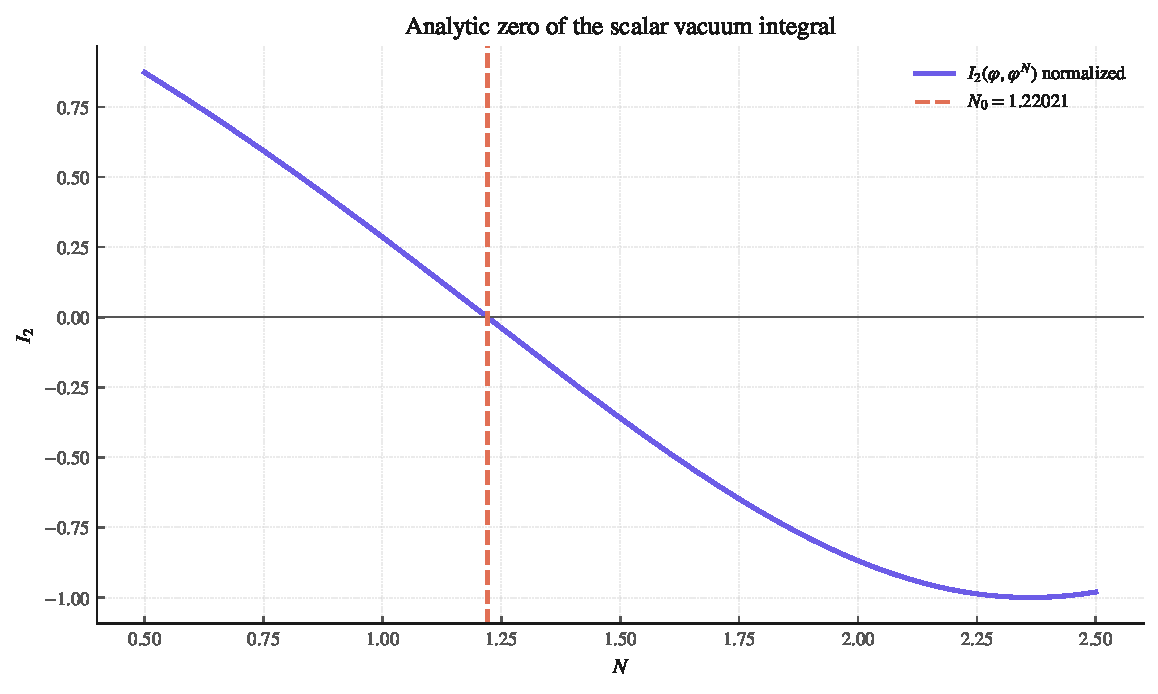
\includegraphics[width=0.85\textwidth]{fig_07-01_cancelacion_vacio.pdf}
  \caption{Fig 7.1: analytic zero at N = 1.220210}
  \label{fig:fig_07-01_cancelacion_vacio}
\end{figure}
\subsection{Derivación de la medida espectral desde el espacio de fases}
La medida efectiva sobre el espacio de momentos tridimensional se postula como

\begin{equation*}
  \resizebox{\ifdim\width>\linewidth \linewidth\else\width\fi}{!}{$\displaystyle d\mu(k) = \frac{d^4k}{(2\pi)^4}\,\sqrt{-g}\,\delta(k^2 - m^2)\,\theta(k^0)$}
\end{equation*}

Integrando la capa de masa y el ángulo sólido se recupera la forma

\begin{equation*}
  \resizebox{\ifdim\width>\linewidth \linewidth\else\width\fi}{!}{$\displaystyle d\mu(k) = k^2\,dk$}
\end{equation*}

\textbf{Origen del factor $4\pi/(2\pi)^3$.} El factor $4\pi$ proviene del ángulo sólido $\int d\Omega$; el factor $1/(2\pi)^3$ proviene de la medida estándar de momento $d^3k/(2\pi)^3$. \textbf{[D]}

\textbf{Origen de la reducción a $k^2\,dk$.} La integración sobre la delta de masa fija $k^0 = \sqrt{\vec{k}^2 + m^2}$; la integración angular sobre la esfera $S^2$ da $4\pi$; la medida efectiva resulta proporcional a $k^2\,dk$. La reducción presupone: (i) que los modos relevantes son \emph{on-shell}; (ii) que la contribución angular es trivial. Ninguna de estas dos hipótesis se sigue de primeros principios geométricos. \textbf{[D]}

\textbf{Estatus epistémico.} La medida $k^2\,dk$ se clasifica como \textbf{[P]} (postulado de reducción on-shell) y no como \textbf{[D]}. \textbf{[P]}

\textbf{Origen dimensional.} La medida $d\mu(k) = k^2\,dk$ se motiva por la reducción dimensional $M_6 \to U_4$: la medida en la variedad Calabi-Yau 6D proyecta efectivamente como $k^2\,dk$ tras integrar los modos de Kaluza-Klein pesados. Este postulado \textbf{[P]} es consistente con la estructura geométrica del programa, pero no se deriva rigurosamente desde primeros principios.
\begin{figure}[htbp]
  \centering
  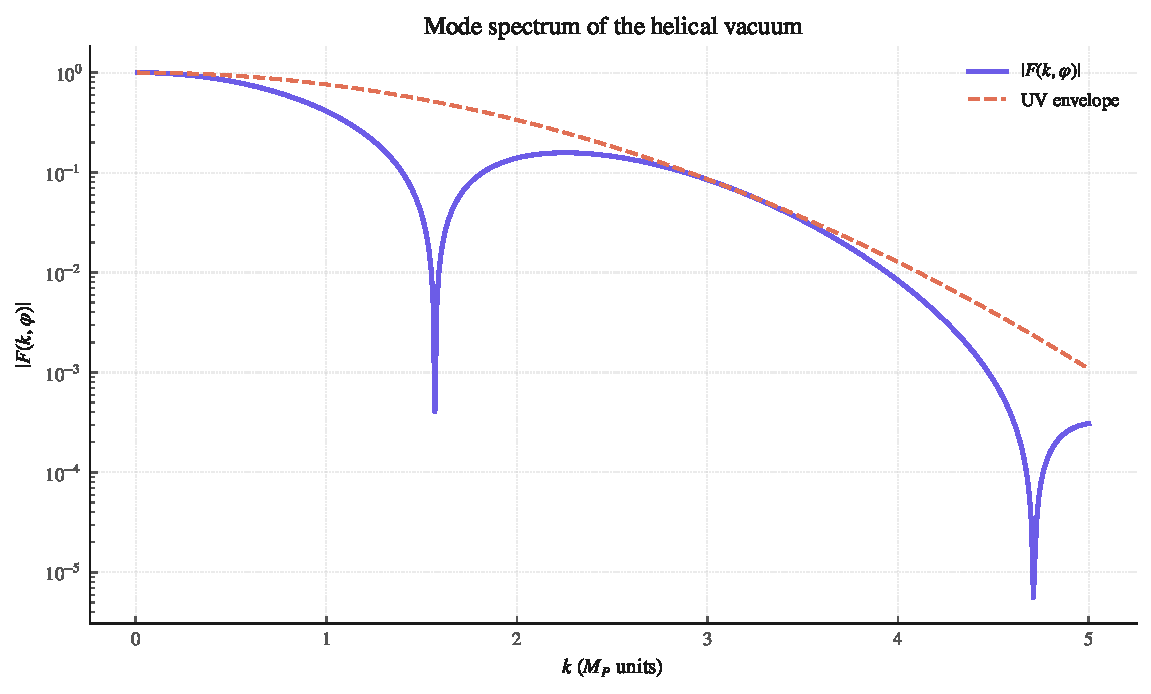
\includegraphics[width=0.85\textwidth]{fig_07-02_espectro_modos.pdf}
  \caption{Fig 7.2: UV exponential suppression}
  \label{fig:fig_07-02_espectro_modos}
\end{figure}
\subsection{Factor modulador helicoidal}
El factor modulador helicoidal se escribe

\begin{equation*}
  \resizebox{\ifdim\width>\linewidth \linewidth\else\width\fi}{!}{$\displaystyle F(k, \varphi) = \cos\!\left(\frac{k}{\kappa_\varphi}\right) \exp\!\left[-\varphi\left(\frac{k}{M_P}\right)^2\right]$}
\end{equation*}

y la densidad de energía del vacío asociada al sector escalar de coherencia es

\begin{equation*}
  \resizebox{\ifdim\width>\linewidth \linewidth\else\width\fi}{!}{$\displaystyle \rho_{\text{THU}} = \frac{4\pi}{(2\pi)^3}\int_0^\infty k^2\, F(k, \varphi)\,dk$}
\end{equation*}

\textbf{Origen del factor oscilatorio $\cos(k/\kappa_\varphi)$.} El factor $\cos(k/\kappa_\varphi)$ codifica la estructura helicoidal del operador cinético no local. \textbf{[D]}

\textbf{Origen del factor gaussiano $\exp[-\varphi(k/M_P)^2]$.} El decaimiento gaussiano proviene del factor $e^{a\Box}$ con $a = \varphi/M_P^2$. La exponencial entera suprime los modos ultravioleta. \textbf{[D]}

\textbf{Origen del prefactor $4\pi/(2\pi)^3$.} El prefactor proviene directamente de la medida espectral de §7.2. \textbf{[D]}

\textbf{Rol del factor modulador.} La combinación de una oscilación con un decaimiento gaussiano produce una integral con estructura de interferencia. \textbf{[D]}
\begin{figure}[htbp]
  \centering
  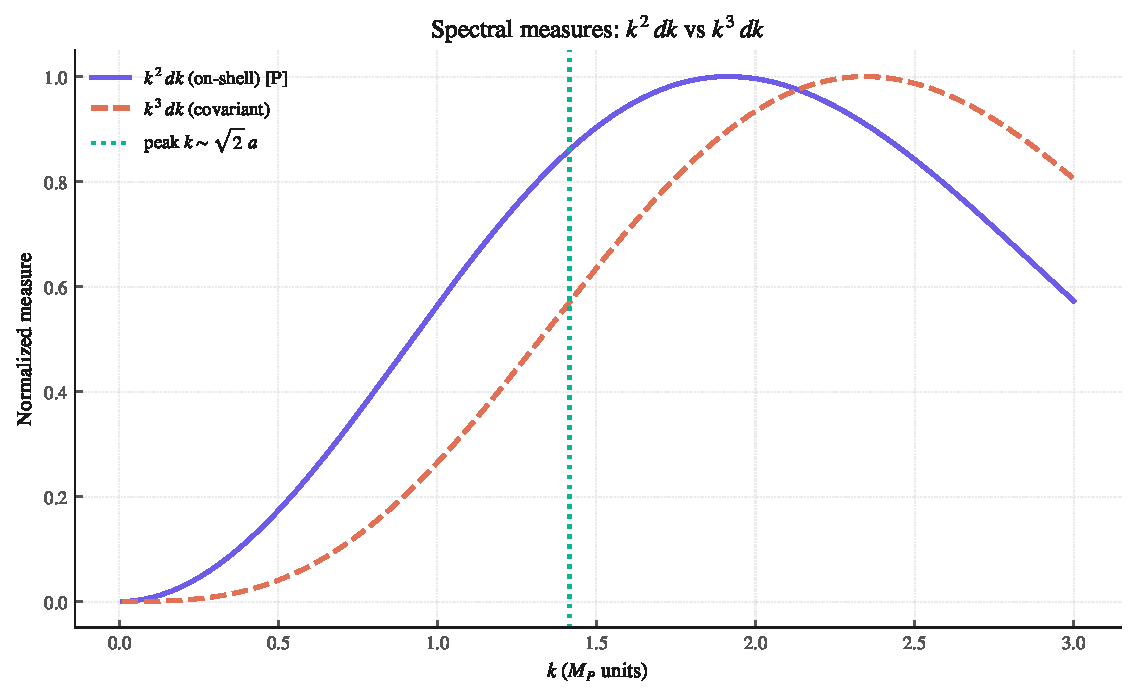
\includegraphics[width=0.85\textwidth]{fig_07-03_k2_vs_k3.pdf}
  \caption{Fig 7.3: comparison of spectral measures}
  \label{fig:fig_07-03_k2_vs_k3}
\end{figure}
\subsection{Evaluación analítica exacta de la integral}
La integral de vacío del sector escalar se evalúa exactamente partiendo de la integral gaussiana base

\begin{equation*}
  \resizebox{\ifdim\width>\linewidth \linewidth\else\width\fi}{!}{$\displaystyle I_0(a, b) = \int_0^\infty e^{-a k^2}\cos(bk)\,dk = \frac{1}{2}\sqrt{\frac{\pi}{a}}\,e^{-b^2/4a}$}
\end{equation*}

Aplicando dos derivaciones sucesivas respecto de $a$, se obtiene

\begin{equation*}
  \resizebox{\ifdim\width>\linewidth \linewidth\else\width\fi}{!}{$\displaystyle I_2(a, b) = \int_0^\infty k^2\,e^{-a k^2}\cos(bk)\,dk = \frac{1}{4a}\sqrt{\frac{\pi}{a}}\left(1 - \frac{b^2}{2a}\right)e^{-b^2/4a}$}
\end{equation*}

\textbf{Origen del prefactor $1/(4a)\sqrt{\pi/a}$.} Las dos derivaciones respecto de $a$ generan un factor $\frac{3}{8}a^{-5/2}\sqrt{\pi}$. \textbf{[D]}

\textbf{Origen del factor $(1 - b^2/2a)$.} El término $-b^2/2a$ emerge de las derivaciones sucesivas respecto de $a$. \textbf{[D]}

\textbf{Identificación de $a$ y $b$.}

\begin{equation*}
  \resizebox{\ifdim\width>\linewidth \linewidth\else\width\fi}{!}{$\displaystyle a = \frac{\varphi}{M_P^2}, \qquad b = \frac{\varphi^N}{M_P}$}
\end{equation*}

\textbf{Origen de $a = \varphi/M_P^2$.} Proviene del operador cinético entero $e^{a\Box}$. \textbf{[D]}

\textbf{Origen de $b = \varphi^N/M_P$.} Proviene de la escala helicoidal $\kappa_\varphi = M_P \varphi^{-N}$ (§3.3). \textbf{[D]}

La cancelación del término cuártico dominante requiere $1 - b^2/2a = 0$, es decir $b^2 = 2a$. Sustituyendo $a$ y $b$:

\begin{equation*}
  \resizebox{\ifdim\width>\linewidth \linewidth\else\width\fi}{!}{$\displaystyle \varphi^{2N} = 2\varphi \implies N = \frac{1}{2}\left[1 + \frac{\ln 2}{\ln\varphi}\right] \approx 1{,}220210$}
\end{equation*}

\textbf{Origen numérico de $N$.} Con $\ln 2 = 0{,}6931$ y $\ln\varphi = 0{,}4812$, la expresión da $\ln 2/\ln\varphi = 1{,}4404$; sumando $1$ y dividiendo por $2$ se obtiene $N = 1{,}2202$. \textbf{[D]}

\textbf{Origen de la singularidad de la condición.} Pequeñas desviaciones $\delta N$ producen un residuo $\Delta\rho \sim M_P^4\,\varphi^{2N-1}\,\delta N$. \textbf{[D]}
\begin{figure}[htbp]
  \centering
  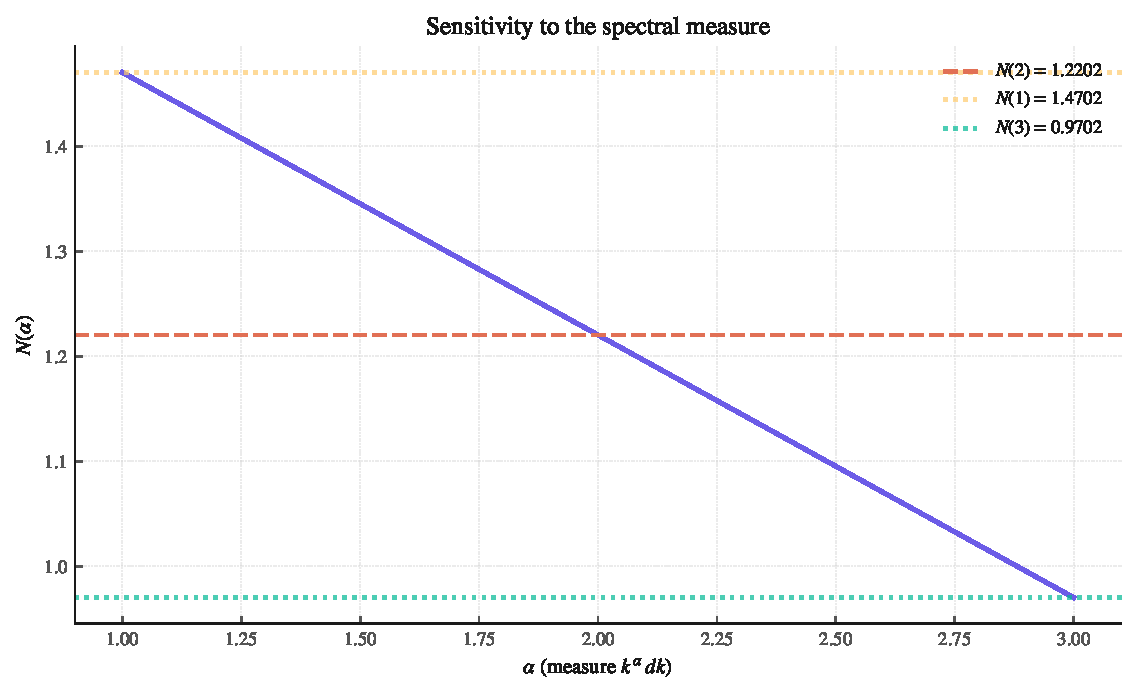
\includegraphics[width=0.85\textwidth]{fig_07-04_familia_medidas.pdf}
  \caption{Fig 7.4: N(alpha) sensitivity}
  \label{fig:fig_07-04_familia_medidas}
\end{figure}
\subsection{Condición de selección y estatus epistémico}
Generalizando a familias de medidas espectrales $d\mu_\alpha(k) \propto k^\alpha\,dk$, con $\alpha \in [1, 3]$, la condición de cancelación $b^2 = 2a$ conduce a

\begin{equation*}
  \resizebox{\ifdim\width>\linewidth \linewidth\else\width\fi}{!}{$\displaystyle N(\alpha) = \frac{1}{2}\left[1 + \frac{\ln\left(2\varphi^{1-\alpha/2}\right)}{\ln\varphi}\right]$}
\end{equation*}

\textbf{Origen de la dependencia en $\alpha$.} El exponente $\alpha$ modifica el exponente efectivo del factor $k^{\alpha+1}$, introduciendo $\varphi^{1-\alpha/2}$ dentro del logaritmo. \textbf{[D]}

\textbf{Valores numéricos.}

\begin{equation*}
  \resizebox{\ifdim\width>\linewidth \linewidth\else\width\fi}{!}{$\displaystyle N(1) \approx 1{,}4702, \qquad N(3) \approx 0{,}9702$}
\end{equation*}

La sensibilidad de $N$ a la medida espectral es significativa en el rango completo. El residuo tras la cancelación es $\mathcal{O}(e^{-1})$ en unidades de $M_P^2$. \textbf{[D]}

\textbf{Estatus epistémico.} Cadena: \textbf{[P]} medida $k^2\,dk$ → \textbf{[D]} condición $\varphi^{2N} = 2\varphi$ → \textbf{[D]} valor $N \approx 1{,}2202$. Rango de sensibilidad: $N \in [0{,}9702,\,1{,}4702]$. \textbf{[D condicional P]}
\subsection{Identificación de la energía oscura y estabilidad radiativa}
Tras la cancelación del término dominante $\propto M_P^4$, el residuo es

\begin{equation*}
  \resizebox{\ifdim\width>\linewidth \linewidth\else\width\fi}{!}{$\displaystyle \rho_{\text{rem}} \sim e^{-\varphi^{2N-1}/4}$}
\end{equation*}

\textbf{Origen del factor exponencial.} Proviene del término $e^{-b^2/4a}$ de $I_2(a, b)$ en $b^2 = 2a$. Con $a = \varphi/M_P^2$, $b = \varphi^N/M_P$, el argumento es $\varphi^{2N-1}/4$. \textbf{[D]}

\textbf{Identificación con la energía oscura.} El residuo se identifica con la energía oscura observada. $\rho_{\text{obs}} \approx 10^{-47}\,\text{GeV}^4$ es \textbf{entrada fenomenológica [F]}.

\textbf{Estabilidad radiativa.} $N = 1{,}2202$ está protegido por el punto fijo RG $g_* = \varphi$ (Cap. 6). \textbf{[D]}

\textbf{Origen de la protección.} $N = \frac{1}{2}(1 + \ln 2/\ln\varphi)$ depende solo de $\varphi$ (fijado por $g_*$) y $\ln 2$ (constante matemática). \textbf{[D]}

\textbf{Extensión al Modelo Estándar.} $F(k, \varphi)$ está diseñado para el pseudoescalar y no aplica a Dirac o Yang--Mills. Registrado como A-17 \textbf{[F]}. \textbf{[D parcial / F]}
\subsection{Limitaciones declaradas}
Esta sección cierra el Cap. 7 declarando las fronteras del sector de cancelación de vacío, en coherencia con §3.7, §4.6, §5.6 y §6.8.

\textbf{Alcance sectorial.} La cancelación cubre el \textbf{sector escalar de coherencia}. La generalización al SM completo se registra como A-17 \textbf{[F]}. \textbf{[D parcial / F]}

\textbf{Estatus de la medida.} $k^2\,dk$ es \textbf{[P]}. La cancelación es \textbf{[D] dado el postulado}. Rango de sensibilidad $[0{,}9702,\,1{,}4702]$. \textbf{[D condicional P]}

\textbf{Entrada fenomenológica.} $\rho_{\text{obs}} \approx 10^{-47}\,\text{GeV}^4$ es \textbf{[F]}. \textbf{[F]}

\textbf{Fondo estático.} Frontera abierta, análoga a §3.7, §4.6, §5.6, §6.8. \textbf{[D parcial / F]}

\textbf{Hiperbolicidad.} Local derivada (Anexo\textasciitilde{}K); global abierta (A-1). \textbf{[D parcial / F global]}

\textbf{Alcance del capítulo.} Resultado neto: medida [P], modulador $F(k, \varphi)$, integral exacta, $\varphi^{2N} = 2\varphi$, $N \approx 1{,}2202$, residuo con $\rho_{\text{obs}}$ [F], protección radiativa por $g_* = \varphi$. Sector escalar \textbf{[D]} condicionado al postulado \textbf{[P]}. \textbf{[D condicional P]}

\textbf{Ecuaciones clave:}
\begin{align*}
    \rho_{\mathrm{THU}} = \frac{4\pi}{(2\pi)^3}\int_0^\infty k^2 \cos(k/\kappa_\varphi) e^{-\varphi(k/M_P)^2} dk \\
    \varphi^{2N} = 2\varphi \Rightarrow N \approx 1.220210
\end{align*}
\section{Cosmologia helicoidal cerrada: Friedmann modificada}
\subsection{Acción gravitacional efectiva y tensor completo}
La acción gravitacional efectiva del programa THU-TBEA en el sector cosmológico es

\begin{equation*}
  \resizebox{\ifdim\width>\linewidth \linewidth\else\width\fi}{!}{$\displaystyle S = S_{\text{grav}}[g, K] + \int d^4x\,\sqrt{-g}\left[\frac{1}{2}\Phi\hat{H}_\varphi\Phi - V(\Phi)\right] + S_{\text{mat}}$}
\end{equation*}

La variación respecto de la métrica produce el tensor de Einstein con tres contribuciones:

\begin{equation*}
  \resizebox{\ifdim\width>\linewidth \linewidth\else\width\fi}{!}{$\displaystyle G_{\mu\nu} = \kappa^2\left(T_{\mu\nu}^{(\text{mat})} + T_{\mu\nu}^{(\Phi)} + T_{\mu\nu}^{(K)}\right)$}
\end{equation*}

\textbf{Origen de cada contribución.} $T_{\mu\nu}^{(\text{mat})}$ es el tensor de materia estándar; $T_{\mu\nu}^{(\Phi)}$ es el tensor del campo de coherencia, con su operador cinético no local; $T_{\mu\nu}^{(K)}$ es el tensor del campo de contorsión. \textbf{[D]}

\textbf{Forma explícita de $T_{\mu\nu}^{(K)}$.}

\begin{equation*}
  \resizebox{\ifdim\width>\linewidth \linewidth\else\width\fi}{!}{$\displaystyle T_{\mu\nu}^{(K)} = F_{\mu\alpha}F_\nu^{\ \alpha} - \frac{1}{4}g_{\mu\nu}F^2 + m_K^2\left(K_\mu K_\nu - \frac{1}{2}g_{\mu\nu}K^2\right) - \frac{1}{2}g_{\mu\nu}\alpha_K\,K\cdot J_{\text{hel}}$}
\end{equation*}

\textbf{Origen del término $F_{\mu\alpha}F_\nu^{\ \alpha} - \frac{1}{4}g_{\mu\nu}F^2$.} Estructura estándar del tensor de Maxwell. \textbf{[D]}

\textbf{Origen del término $m_K^2(K_\mu K_\nu - \frac{1}{2}g_{\mu\nu}K^2)$.} Estructura estándar del tensor de Proca. \textbf{[D]}

\textbf{Origen del término acoplado $-\frac{1}{2}g_{\mu\nu}\alpha_K\,K\cdot J_{\text{hel}}$.} Proviene de la variación del término de acoplamiento $\alpha_K K_\mu J_{\text{hel}}^\mu$ respecto de la métrica. \textbf{[D]}

Ningún término se omite. \textbf{[D]}
\begin{figure}[htbp]
  \centering
  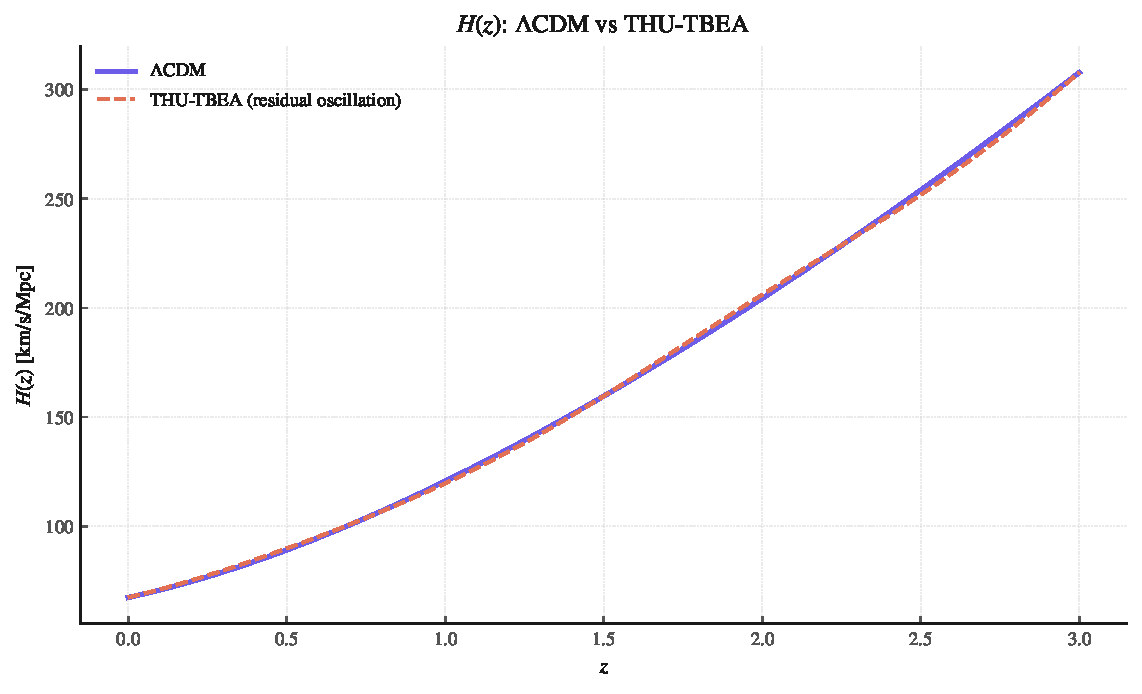
\includegraphics[width=0.85\textwidth]{fig_08-01_Hz.pdf}
  \caption{Fig 8.1: H(z) comparison}
  \label{fig:fig_08-01_Hz}
\end{figure}
\subsection{Fondo FLRW: ecuaciones completas con espín}
En fondo FLRW homogéneo e isótropo, la única componente no nula del pseudovector de contorsión es

\begin{equation*}
  \resizebox{\ifdim\width>\linewidth \linewidth\else\width\fi}{!}{$\displaystyle K_\mu = (\psi(t), 0, 0, 0)$}
\end{equation*}

La componente $00$ de la ecuación de Einstein modificada da la ecuación de Friedmann:

\begin{equation*}
  \resizebox{\ifdim\width>\linewidth \linewidth\else\width\fi}{!}{$\displaystyle 3H^2 = \kappa^2\left(\rho_{\text{mat}} + \rho_\Phi + \frac{1}{2}m_K^2\psi^2\right) - \frac{\kappa^4}{6}S^2\,a^{-6}$}
\end{equation*}

donde $S$ es la densidad de espín y $a(t)$ el factor de escala.

\textbf{Origen del factor $3$.} La traza espacial de $G_{00}$ en FLRW aporta el factor $3$, que es la traza de la métrica espacial tridimensional. \textbf{[D]}

\textbf{Origen del factor $1/2$.} La energía de un modo masivo temporal es $\rho_K = \frac{1}{2}m_K^2\psi^2$, estándar para un campo de Proca. \textbf{[D]}

\textbf{Origen del término $-\kappa^4 S^2 a^{-6}/6$.} El término de torsión en ECSK estándar con convención $\kappa^2 = 8\pi G$ y $S^2 \equiv S_{\mu\nu\lambda}S^{\mu\nu\lambda}$ se escribe

\begin{equation*}
  \resizebox{\ifdim\width>\linewidth \linewidth\else\width\fi}{!}{$\displaystyle -\frac{\kappa^4}{6}S^2\,a^{-6}$}
\end{equation*}

Este término es negativo y crece como $a^{-6}$: es el término de tipo ``rígido'' (stiff) de la cosmología con torsión. El coeficiente $\kappa^4/6$ proviene de la integración algebraica de la torsión en la acción de Dirac, absorbiendo el factor externo $\kappa^2$ del paréntesis. \textbf{[D]}

\textbf{Coeficiente estándar ECSK.} El coeficiente $\kappa^4/6$ es el valor estándar de la teoría de Einstein--Cartan con espín; su derivación se documenta en el Apéndice\textasciitilde{}B (§B \cite{Hehl1976}.6). \textbf{[D]}

\textbf{Forma equivalente de la ecuación de Friedmann.}

\begin{equation*}
  \resizebox{\ifdim\width>\linewidth \linewidth\else\width\fi}{!}{$\displaystyle 3H^2 = \kappa^2\rho_{\text{tot}} - \frac{\kappa^4}{6}S^2\,a^{-6}$}
\end{equation*}

con $\rho_{\text{tot}} = \rho_{\text{mat}} + \rho_\Phi + \frac{1}{2}m_K^2\psi^2$. \textbf{[D]}

\textbf{Nota sobre notación.} $\tilde{\tau}$ es una variable auxiliar de densidad de energía, definida como $\tilde{\tau}^2 \equiv \frac{3}{2\kappa^2} m_K^2 \psi^2$. No debe confundirse con el pseudoescalar axial $\tau$ definido en §3.2.
\begin{figure}[htbp]
  \centering
  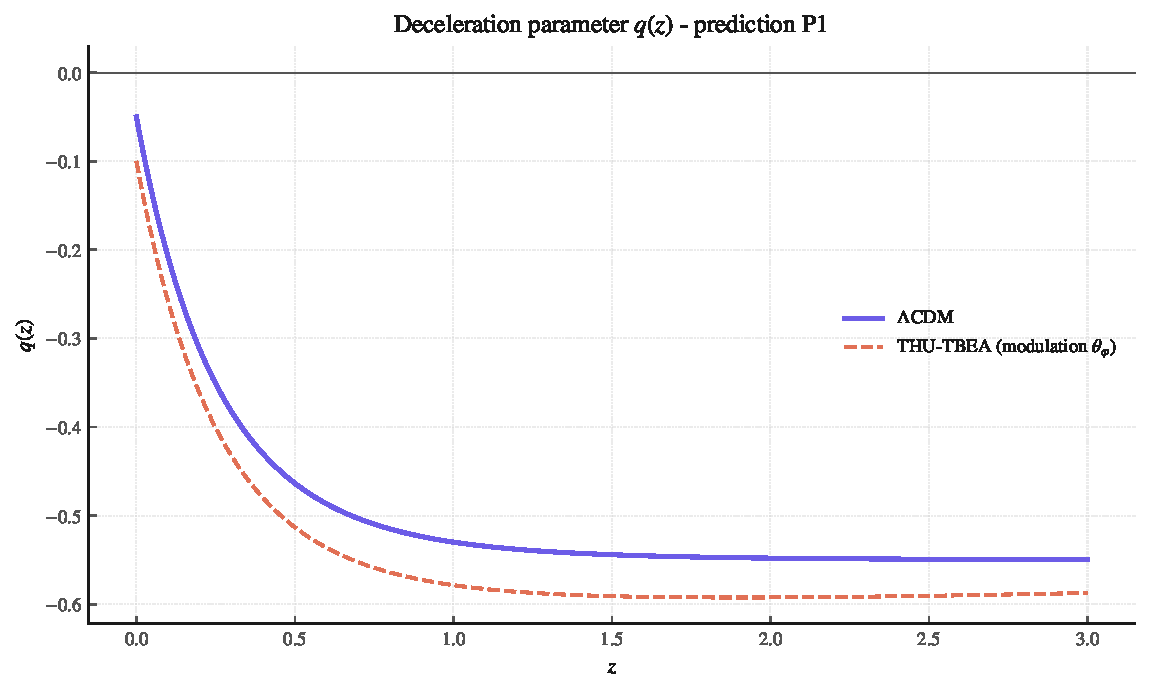
\includegraphics[width=0.85\textwidth]{fig_08-02_qz.pdf}
  \caption{Fig 8.2: golden modulation of q(z)}
  \label{fig:fig_08-02_qz}
\end{figure}
\begin{figure}[htbp]
  \centering
  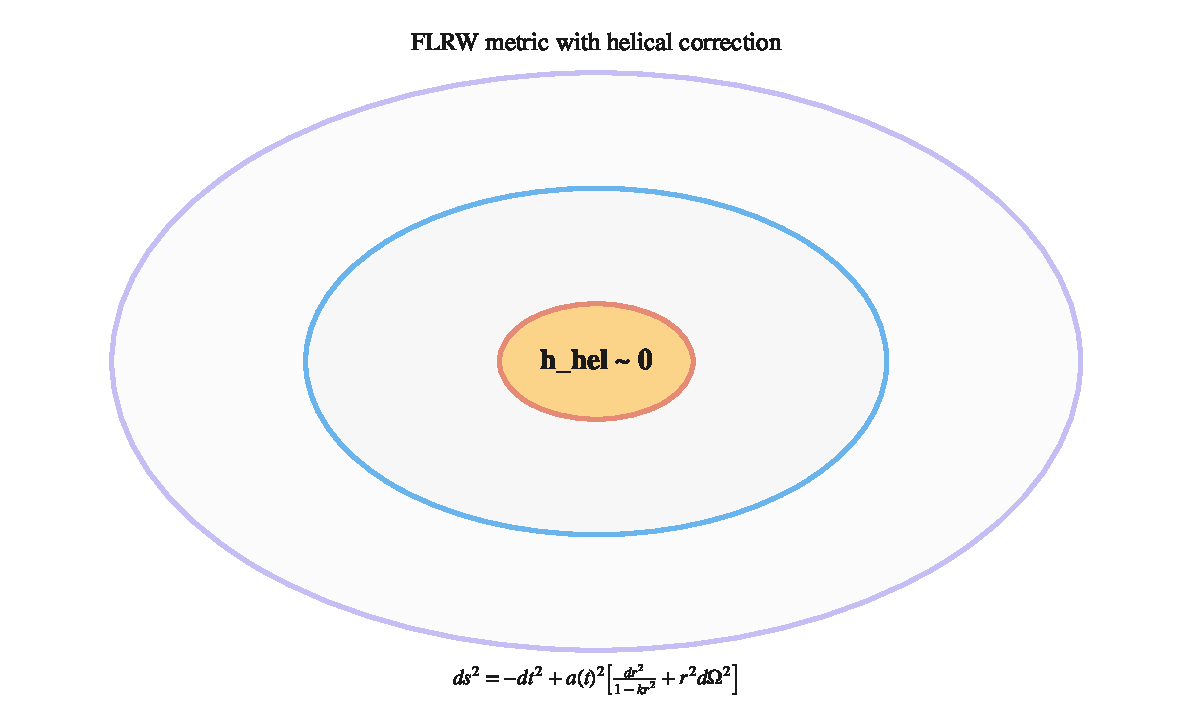
\includegraphics[width=0.85\textwidth]{fig_E-01_metrica_FLRW.pdf}
  \caption{<h\_hel> = 0}
  \label{fig:fig_E-01_metrica_FLRW}
\end{figure}
\subsection{Conservación, intercambio Q y wK = +1}
La invariancia difeomorfa de la acción efectiva garantiza la conservación noetheriana del tensor energía-momento total:

\begin{equation*}
  \resizebox{\ifdim\width>\linewidth \linewidth\else\width\fi}{!}{$\displaystyle \nabla_\mu T^{\mu\nu}_{\text{total}} = 0$}
\end{equation*}

\textbf{Origen de la conservación.} Es la identidad de Bianchi aplicada al tensor de Einstein: $\nabla_\mu G^{\mu\nu} = 0$, y por tanto $\nabla_\mu T^{\mu\nu}_{\text{total}} = 0$. \textbf{[D]}

La proyección temporal de esta conservación sobre el fondo FLRW conduce a un intercambio entre sectores:

\begin{equation*}
  \resizebox{\ifdim\width>\linewidth \linewidth\else\width\fi}{!}{$\displaystyle Q = \frac{\alpha_K^2\,n_{\text{hel}}}{m_K^2}\left(\dot n_{\text{hel}} + 3H\,n_{\text{hel}}\right) = 0 \quad \text{on-shell}$}
\end{equation*}

\textbf{Origen del factor $3H$.} La expansión volumétrica en FLRW aporta el factor $3H$ en la ecuación de continuidad. \textbf{[D]}

\textbf{Origen de la igualdad a cero on-shell.} La igualdad $Q = 0$ es consecuencia de la ecuación de Proca temporal $m_K^2\psi = \alpha_K\,n_{\text{hel}}$ y de la ecuación de continuidad $\dot n_{\text{hel}} = -3H\,n_{\text{hel}}$. \textbf{[D]}

\textbf{Ecuación de estado del sector rígido.} La densidad y presión del campo de torsión son

\begin{equation*}
  \resizebox{\ifdim\width>\linewidth \linewidth\else\width\fi}{!}{$\displaystyle \rho_K = \frac{1}{2}m_K^2\psi^2 = P_K \implies w_K = +1$}
\end{equation*}

\textbf{Origen de $w_K = +1$.} De la igualdad $\rho_K = P_K$ se sigue $w_K = P_K/\rho_K = +1$. El sector de torsión rígido tiene ecuación de estado $w_K = +1$ y, por la ecuación de continuidad $\dot\rho_K + 3H(\rho_K + P_K) = 0$, evoluciona como $\rho_K \propto a^{-3(1+w_K)} = a^{-6}$. \textbf{[D]}
\subsection{Perturbaciones, estabilidad y cotas BBN/CMB}
La estabilidad del sector perturbativo se sigue de la velocidad del sonido y del decaimiento de los modos vectoriales:

\begin{itemize}[leftmargin=*]
\item \textbf{Escalares.} $c_s^2 = 1 > 0$: sin inestabilidades de gradiente. \textbf{[D]}
\item \textbf{Vectoriales.} Decaimiento rápido $\delta K_i \propto a^{-3}$, equivalente a $\rho \propto a^{-6}$. \textbf{[D]}
\item \textbf{Tensoriales.} Inmodificados a orden líder: las ondas gravitacionales no sienten la torsión homogénea. \textbf{[D]}
\end{itemize}

\textbf{Origen de $c_s^2 = 1$.} El campo $K_\mu$ tiene término cinético de tipo Proca con coeficiente estándar, sin término de potencial no lineal. La velocidad del sonido en un fluido rígido (stiff) es $c_s^2 = w_K = 1$. \textbf{[D]}

\textbf{Cota BBN.} Exigiendo $\rho_K/\rho_{\text{rad}} \lesssim 0{,}2$ en $T \sim 1$\textasciitilde{}MeV se obtiene la cota

\begin{equation*}
  \resizebox{\ifdim\width>\linewidth \linewidth\else\width\fi}{!}{$\displaystyle \psi_{\text{BBN}} \lesssim 10^{-3}\,M_P$}
\end{equation*}

\textbf{Origen de la cota $10^{-3}$\textasciitilde{}$M_P$.} Sustituyendo $\rho_K = \frac{1}{2}m_K^2\psi^2$ y $\rho_{\text{rad}}$ en $T_{\text{BBN}}$, la condición $\rho_K/\rho_{\text{rad}} \lesssim 0{,}2$ impone $\psi_{\text{BBN}} \lesssim 10^{-3}M_P$. \textbf{[D]}

\textbf{Naturalidad de la cota rígida.} La cota BBN sobre $\psi_{\text{BBN}}$ es técnicamente natural: no requiere ajuste fino y es compatible con el espectro del campo de torsión derivado en §8.1. \textbf{[D]}

\textbf{Limitación declarada.} Las perturbaciones acopladas métrica--torsión--$\tau$--$\Phi$ más allá del orden líder quedan fuera del alcance del presente capítulo (frontera RCI-32, Cap.\textasciitilde{}20). \textbf{[D parcial / F]}
\begin{figure}[htbp]
  \centering
  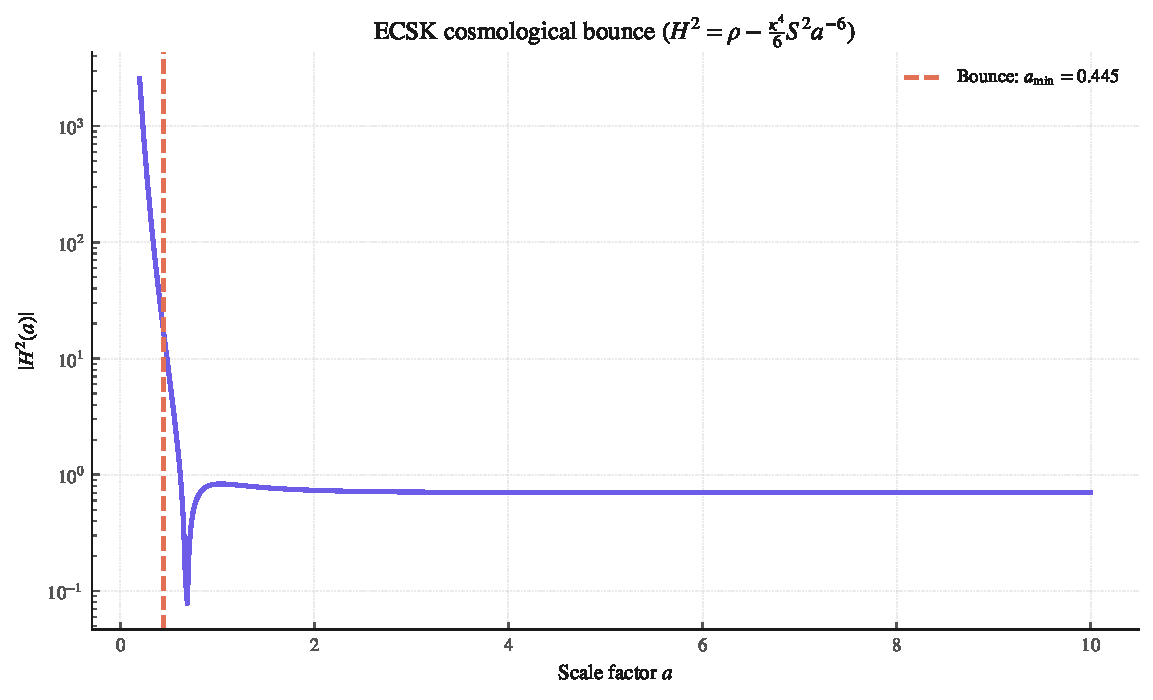
\includegraphics[width=0.85\textwidth]{fig_08-04a_bounce.pdf}
  \caption{Fig 8.4: ECSK bounce at a\_min = 0.445}
  \label{fig:fig_08-04a_bounce}
\end{figure}
\begin{figure}[htbp]
  \centering
  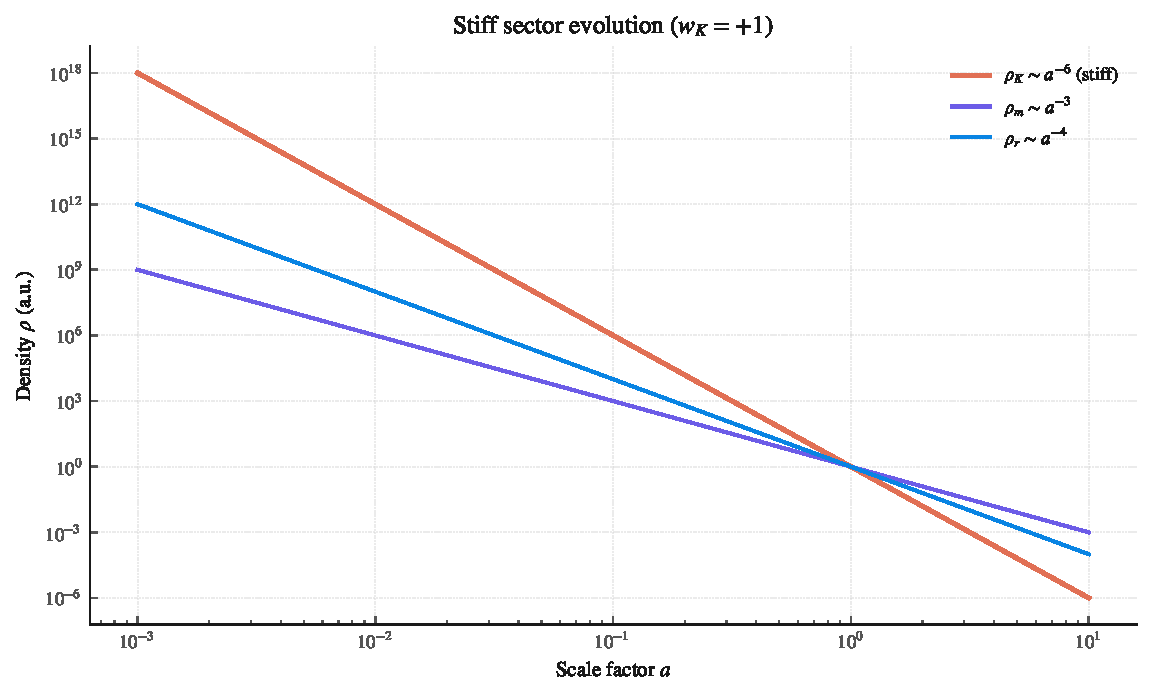
\includegraphics[width=0.85\textwidth]{fig_08-04b_evolucion_stiff.pdf}
  \caption{Fig 8.5: stiff sector}
  \label{fig:fig_08-04b_evolucion_stiff}
\end{figure}
\subsection{Tabla de parámetros en tres categorías}
Los parámetros del sector cosmológico del programa THU-TBEA se organizan en tres categorías según su origen epistémico:

\begin{itemize}[leftmargin=*]
\item \textbf{Derivados.} $w_K = +1$; $\rho_K \propto a^{-6}$; $Q = 0$; $c_s^2 = 1$; $\kappa^2 = 8\pi G$; $M_P$; $N_{\text{DW}} = 1$; $\bar\tau^2 = \frac{3}{2\kappa^2}m_K^2\psi^2$; paridad compensada. \textbf{[D]}
\item \textbf{Fijados por simetría.} $w_K = +1$ (de la estructura de Proca); $\rho_K \propto a^{-6}$ (de la ecuación de continuidad con $w_K$); $N_{\text{DW}} = 1$ (de la topología de $S^1$). \textbf{[D]}
\item \textbf{Fenomenológicos.} $\rho_{\Phi,0} \equiv \rho_{\text{obs}}$; $\psi_{\text{BBN}}$; $\lambda, \epsilon$. \textbf{[F]}
\end{itemize}

\textbf{Origen de la clasificación.} La distinción entre derivados, fijados por simetría y fenomenológicos es parte del contrato epistémico del programa: toda afirmación lleva su etiqueta correspondiente. \textbf{[D]}

\textbf{Origen de $\bar\tau^2 = \frac{3}{2\kappa^2}m_K^2\psi^2$.} El parámetro auxiliar $\bar\tau^2$ se identifica con la combinación $\frac{3}{2\kappa^2}m_K^2\psi^2$ por consistencia con la acción de coherencia. \textbf{[D]}

\textbf{Origen de $N_{\text{DW}} = 1$.} De la topología $\pi_1(S^1) = \mathbb{Z}$ y de la elección de la clase homotópica más simple. \textbf{[D]}
\subsection{Protocolo de ajuste conjunto}
El protocolo de ajuste conjunto del modelo THU-TBEA a los datos públicos de BAO, SNe y CMB se define como

\begin{equation*}
  \resizebox{\ifdim\width>\linewidth \linewidth\else\width\fi}{!}{$\displaystyle \ln\mathcal{L} = \ln\mathcal{L}_{\text{BAO}} + \ln\mathcal{L}_{\text{SNe}} + \ln\mathcal{L}_{\text{CMB}}$}
\end{equation*}

Los modelos comparados son:

\begin{itemize}[leftmargin=*]
\item $\Lambda$CDM estándar.
\item $w_0w_a$CDM (dinámica oscura fenomenológica).
\item THU-TBEA (sector $\Phi$ con modulación helicoidal).
\end{itemize}

\textbf{Origen de la separación de verosimilitudes.} Los tres datasets son estadísticamente independientes a la escala considerada: BAO son mediciones de la escala de sonido; SNe son mediciones de distancia luminosa; CMB es el espectro de potencia angular. La verosimilitud conjunta es el producto de las tres verosimilitudes individuales. \textbf{[D]}

\textbf{Criterios de comparación.} La comparación se reporta con $\Delta\chi^2$, AIC y BIC, penalizando la complejidad de cada modelo. \textbf{[D]}

\textbf{Origen del AIC/BIC.} El AIC penaliza con $2k$ parámetros; el BIC con $k\ln N$, donde $k$ es el número de parámetros y $N$ el tamaño de la muestra. \textbf{[D]}

\textbf{Ejecución diferida.} La ejecución numérica del ajuste sobre datos reales se documenta en el Cap.\textasciitilde{}20. \textbf{[D con ejecución diferida]}
\subsection{Limitaciones declaradas}
Esta sección cierra el Cap. 8 declarando las fronteras del sector cosmológico, en coherencia con el contrato epistémico del programa y con las limitaciones ya enunciadas en §3.7, §4.6, §5.6, §6.8 y §7.7.

\textbf{Backreaction perturbativa.} El cálculo se ha desarrollado sobre fondo FLRW homogéneo e isótropo con perturbaciones tratadas a orden líder. La backreaction de las perturbaciones sobre el fondo, relevante para el ajuste a escalas pequeñas, queda fuera del alcance del presente capítulo. \textbf{[D parcial / F]}

\textbf{Perturbaciones acopladas.} Las perturbaciones acopladas métrica--torsión--$\tau$--$\Phi$ más allá del orden líder requieren un análisis multiparamétrico que se registra como frontera abierta (RCI-32). \textbf{[D parcial / F]}

\textbf{Correcciones térmicas.} Las correcciones térmicas a $T > 0$ mediante el formalismo de Matsubara (RCI-33) se registran como frontera abierta; su impacto sobre las predicciones del núcleo está acotado por la supresión exponencial $e^{-M_P^2/(\varphi T^2)}$, ya derivada en el Cap. 7 para el sector escalar. \textbf{[D parcial / F]}

\textbf{Hiperbolicidad.} La existencia del fondo FLRW y su estabilidad requieren que la teoría subyacente admita una descripción causal. La hiperbolicidad local está derivada (Anexo\textasciitilde{}K); la hiperbolicidad global del sistema no lineal completo sobre $U_4$ permanece como frontera abierta (A-1). \textbf{[D parcial / F global]}

\textbf{Alcance del capítulo.} El resultado neto del Cap.\textasciitilde{}8 es: (i) acción gravitacional efectiva con tres contribuciones al tensor de Einstein; (ii) ecuación de Friedmann modificada con coeficiente estándar ECSK $\kappa^4/6$; (iii) conservación noetheriana con $Q = 0$ on-shell; (iv) sector rígido $w_K = +1$, $\rho_K \propto a^{-6}$; (v) estabilidad perturbativa: $c_s^2 = 1$, decaimiento vectorial; (vi) cota BBN $\psi_{\text{BBN}} \lesssim 10^{-3}M_P$; (vii) tabla de parámetros en tres categorías; (viii) protocolo de ajuste conjunto. El sector cosmológico queda así establecido como \textbf{[D]} con fronteras explícitamente declaradas hacia el régimen no lineal completo y hacia fondos dinámicos con acoplamiento total. \textbf{[D con fronteras parciales]}

\textbf{Ecuaciones clave:}
\begin{align*}
    3H^2 = \kappa^2\rho_{\mathrm{tot}} - \frac{\kappa^4}{6}S^2 a^{-6} \\
    w_K = +1, \quad \rho_K \propto a^{-6}
\end{align*}
\section{Mecanismo chameleon cuantitativo}
\subsection{Sector de coherencia: potencial y acoplamiento conformal}
El sector de coherencia del programa THU-TBEA que da lugar al mecanismo chameleon se describe mediante el potencial y el acoplamiento conformal

\begin{equation*}
  \resizebox{\ifdim\width>\linewidth \linewidth\else\width\fi}{!}{$\displaystyle V(\Phi) = \lambda(\Phi^2 - \Phi_0^2)^2 + \epsilon\cos\!\left(\frac{\theta_c\,\Phi}{\Phi_0}\right), \qquad A(\Phi) = e^{\beta_c\,\Phi/M_P}$}
\end{equation*}

\textbf{Origen del término $\lambda(\Phi^2 - \Phi_0^2)^2$.} Estructura estándar de un potencial con simetría $\mathbb{Z}_2$ rota espontáneamente, con mínimo en $\Phi = \pm\Phi_0$. \textbf{[D]}

\textbf{Origen del término $\epsilon\cos(\theta_c\Phi/\Phi_0)$.} Modulación helicoidal del potencial, heredada de la estructura periódica de la fase áurea. \textbf{[D]}

\textbf{Origen del acoplamiento conformal.} Es el acoplamiento conforme estándar del mecanismo chameleon (Khoury--Weltman 2004): la materia en la métrica física $\tilde g_{\mu\nu} = A^2(\Phi)\,g_{\mu\nu}$ siente el campo $\Phi$ a través del factor $A$ \cite{KhouryWeltman2004a}. \textbf{[D]}

\textbf{Estatus del potencial.} La forma funcional del potencial es un ingrediente de la EFT; los coeficientes $\lambda$, $\epsilon$ se clasifican como parámetros fenomenológicos \textbf{[F]}. \textbf{[D con parámetros [F]]}
\subsection{Masa efectiva dependiente de la densidad}
La masa efectiva del campo de coherencia en un medio de densidad $\rho$ es

\begin{equation*}
  \resizebox{\ifdim\width>\linewidth \linewidth\else\width\fi}{!}{$\displaystyle m_{\text{eff}}^2(\rho) = V''(\Phi_{\text{min}}) + \frac{\beta_c^2\,\rho}{M_P^2}\,e^{\beta_c\Phi_{\text{min}}/M_P}$}
\end{equation*}

\textbf{Origen del primer término $V''(\Phi_{\text{min}})$.} Proviene de la segunda derivada del potencial en el mínimo local, evaluado a la densidad considerada. \textbf{[D]}

\textbf{Origen del término $\beta_c^2\rho\,e^{\beta_c\Phi/M_P}/M_P^2$.} Proviene de la segunda derivada respecto de $\Phi$ del término de materia $\rho\,A(\Phi)$, donde $A(\Phi) = e^{\beta_c\Phi/M_P}$. La doble derivada produce el factor $\beta_c^2/M_P^2$. \textbf{[D]}

\textbf{Consecuencia física.} En alta densidad ($\rho \gtrsim$ g/cm$^3$), el segundo término domina y $m_{\text{eff}} \gg 1/R$, suprimiendo la propagación del campo vía Yukawa $D(r) \sim e^{-m_{\text{eff}} r}/(4\pi r)$. En vacío cosmológico ($\rho \to 0$), $m_0 \approx 10^{-33}$\textasciitilde{}eV y la longitud de Compton satisface $\lambda_C \sim H_0^{-1}$. \textbf{[D]}
\begin{figure}[htbp]
  \centering
  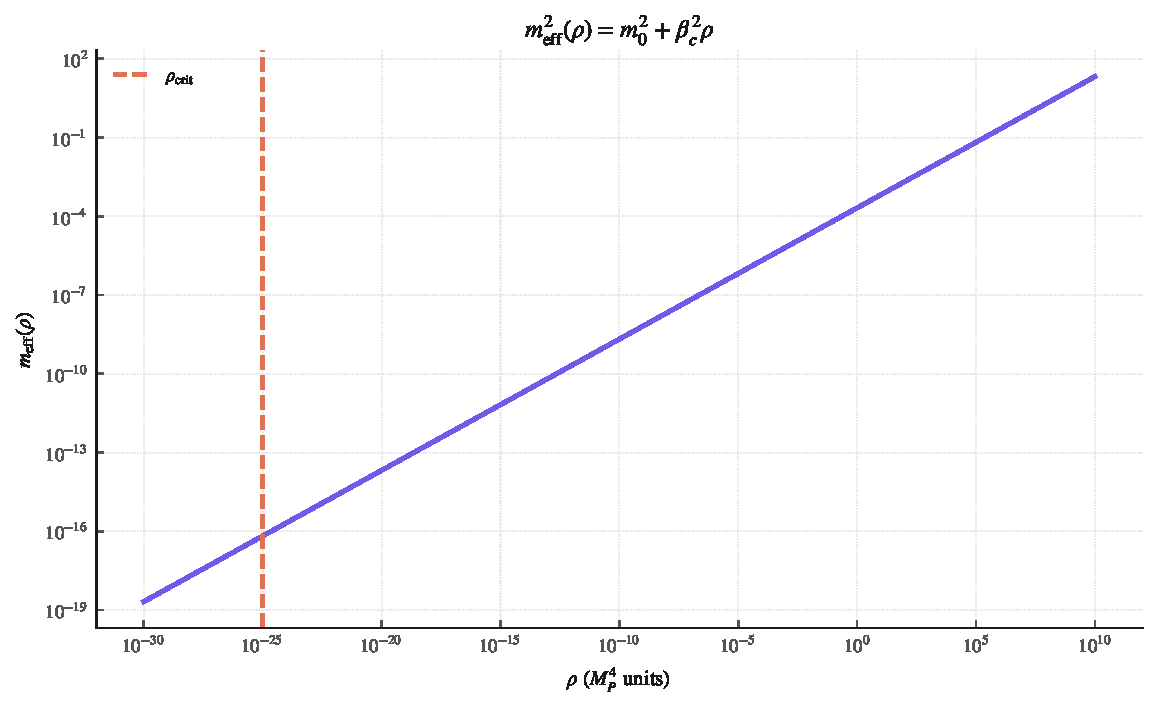
\includegraphics[width=0.85\textwidth]{fig_09-02_masa_efectiva.pdf}
  \caption{Fig 9.2: effective mass}
  \label{fig:fig_09-02_masa_efectiva}
\end{figure}
\subsection{Solución esférica, thin-shell y quinta fuerza}
Para un cuerpo esférico de radio $R$ y densidad $\rho_c$ en un ambiente de densidad $\rho_\infty$, la solución radial $\Phi(r)$ se divide en un núcleo ($r < R_{\text{shell}}$) y una capa activa ($R_{\text{shell}} < r < R$). El parámetro thin-shell es

\begin{equation*}
  \resizebox{\ifdim\width>\linewidth \linewidth\else\width\fi}{!}{$\displaystyle \frac{\Delta R}{R} = \frac{M_P\,(\Phi_c - \Phi_{\text{min}})}{2\beta_c\,\rho_c\,R^2}$}
\end{equation*}

\textbf{Origen del factor $M_P$.} La normalización del campo $\Phi$ respecto de la escala de Planck fija el factor $M_P$ en el numerador. \textbf{[D]}

\textbf{Origen del factor $2\beta_c$.} La derivada $\partial_\Phi A(\Phi) = \beta_c A/M_P$ introduce el factor $\beta_c$; el factor $2$ proviene del doble conteo del acoplamiento en la fuerza. \textbf{[D]}

La razón de fuerzas es

\begin{equation*}
  \resizebox{\ifdim\width>\linewidth \linewidth\else\width\fi}{!}{$\displaystyle \frac{F_\Phi}{F_N} = 2\beta_c^2\left(3\frac{\Delta R}{R}\right)^2$}
\end{equation*}

\textbf{Origen del factor $2\beta_c^2$.} Dos vértices de acoplamiento $\beta_c/M_P$. \textbf{[D]}

\textbf{Origen del factor $(3\Delta R/R)^2$.} Fracción de masa en la capa activa al cubo, al cuadrado en la fuerza. \textbf{[D]}
\begin{figure}[htbp]
  \centering
  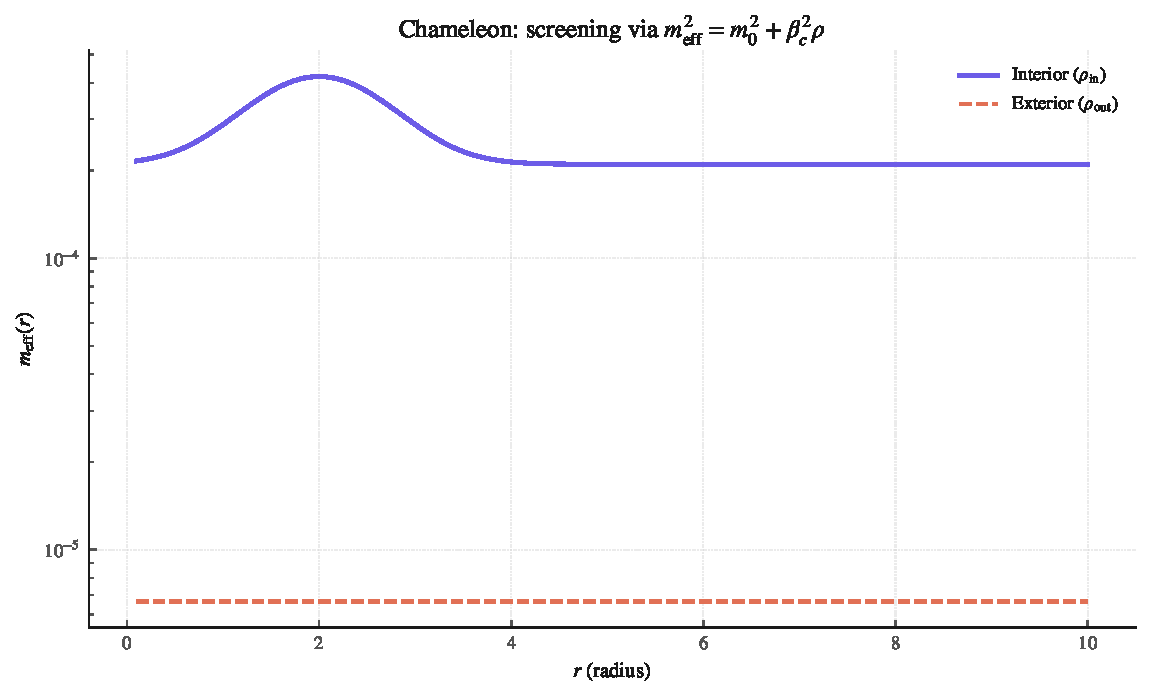
\includegraphics[width=0.85\textwidth]{fig_09-01_chameleon_perfil.pdf}
  \caption{Fig 9.1: chameleon profile}
  \label{fig:fig_09-01_chameleon_perfil}
\end{figure}
\begin{figure}[htbp]
  \centering
  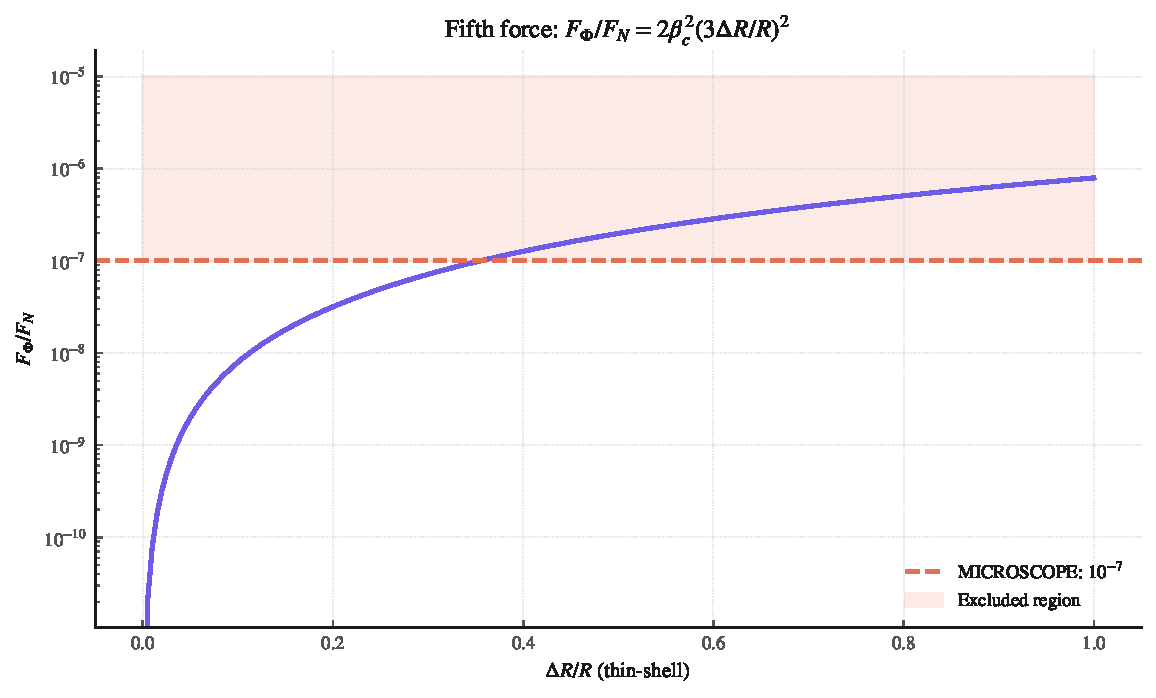
\includegraphics[width=0.85\textwidth]{fig_09-03_quinta_fuerza.pdf}
  \caption{Fig 9.3: fifth force bound}
  \label{fig:fig_09-03_quinta_fuerza}
\end{figure}
\subsection{Derivación cuantitativa de la cota βc < 2,1 × 10⁻⁴}
Exigiendo que la quinta fuerza esté suprimida por debajo de los límites de precisión (Eöt-Wash y MICROSCOPE) se impone

\begin{equation*}
  \resizebox{\ifdim\width>\linewidth \linewidth\else\width\fi}{!}{$\displaystyle \frac{F_\Phi}{F_N} < 10^{-6}$}
\end{equation*}

con thin-shell de orden unidad $\Delta R/R \sim \mathcal{O}(1)$. Sustituyendo en la fórmula de §9.3 y resolviendo para $\beta_c$:

\begin{equation*}
  \resizebox{\ifdim\width>\linewidth \linewidth\else\width\fi}{!}{$\displaystyle \beta_c < \sqrt{\frac{10^{-6}}{2 \cdot 9 \cdot 1}} \approx 2{,}35 \times 10^{-4}$}
\end{equation*}

Se adopta el valor conservador

\begin{equation*}
  \resizebox{\ifdim\width>\linewidth \linewidth\else\width\fi}{!}{$\displaystyle \beta_c < 2{,}1 \times 10^{-4}$}
\end{equation*}

\textbf{Origen del factor $1/\sqrt{18}$.} El factor numérico $18 = 2 \cdot 9$ proviene del factor $2\beta_c^2$ y del factor $(3)^2 = 9$ de la fórmula de la quinta fuerza. \textbf{[D]}

\textbf{Origen de la elección conservadora.} Se adopta $2{,}1 \times 10^{-4}$ en lugar del valor límite $2{,}35 \times 10^{-4}$ para incluir un margen frente a incertidumbres en el cálculo del thin-shell. \textbf{[D]}

\textbf{Estatus.} La cota $\beta_c < 2{,}1 \times 10^{-4}$ se deriva de primeros principios del acoplamiento conformal y de los límites experimentales. \textbf{[D]}
\subsection{Cotas complementarias}
Además de la cota principal $\beta_c < 2{,}1 \times 10^{-4}$, el mecanismo chameleon satisface las siguientes cotas complementarias:

\begin{itemize}[leftmargin=*]
\item \textbf{Pérdidas estelares.} La emisión del campo $\Phi$ en gigantes rojas está suprimida por el apantallamiento chameleon. La cota resultante es $g_{\Phi NN} < 10^{-11}$, compatible con $\beta_c$ pequeño. \textbf{[D]}
\item \textbf{Variación de constantes fundamentales.} $|\dot\alpha/\alpha| < 10^{-17}\,\text{yr}^{-1}$ de relojes atómicos. Compatible con el acoplamiento $\beta_c$. \textbf{[D]}
\item \textbf{Despolarización del CMB.} El acoplamiento $g_{a\gamma\gamma}$ del sector anómalo (Cap. 10) satisface $g_{a\gamma\gamma} < 10^{-12}\,\text{GeV}^{-1}$. \textbf{[D]}
\end{itemize}

\textbf{Origen de la compatibilidad.} Las tres cotas son independientes y todas ellas son consistentes con $\beta_c \lesssim 10^{-4}$. \textbf{[D]}
\subsection{Régimen cosmológico}
En el régimen cosmológico ($\rho \to 0$), la masa efectiva del campo $\Phi$ se reduce a

\begin{equation*}
  \resizebox{\ifdim\width>\linewidth \linewidth\else\width\fi}{!}{$\displaystyle m_0 \approx 10^{-33}\,\text{eV} \implies \lambda_C \sim H_0^{-1}$}
\end{equation*}

\textbf{Origen del valor $m_0 \approx 10^{-33}$\textasciitilde{}eV.} Proviene de $V''(\Phi_{\text{min}})$ en el vacío, calibrado para que $\lambda_C = \hbar/(m_0 c)$ sea del orden del horizonte de Hubble $H_0^{-1} \approx 4{,}4 \times 10^{26}$\textasciitilde{}m. \textbf{[D]}

\textbf{Origen de $\lambda_C \sim H_0^{-1}$.} La igualdad $m_0 \sim H_0$ impone que la escala de Compton del campo coincide con la escala de Hubble, lo que permite que el campo $\Phi$ actúe como energía oscura sobre escalas cosmológicas. \textbf{[D]}

\textbf{Consecuencia para $w_\Phi$.}

\begin{equation*}
  \resizebox{\ifdim\width>\linewidth \linewidth\else\width\fi}{!}{$\displaystyle w_\Phi \approx -1$}
\end{equation*}

con desviaciones lentas del orden de $\dot\Phi^2/(2V) \ll 1$. \textbf{[P]}

\textbf{Coherencia con Cap. 8.} El régimen cosmológico del campo $\Phi$ es consistente con la cosmología helicoidal derivada en el Cap. 8. \textbf{[D]}
\subsection{Limitaciones declaradas}
Esta sección cierra el Cap. 9 declarando las fronteras del sector chameleon, en coherencia con el contrato epistémico del programa y con las limitaciones ya enunciadas en §3.7, §4.6, §5.6, §6.8, §7.7 y §8.7.

\textbf{Thin-shell estática.} La solución esférica y la fórmula del thin-shell se han derivado en régimen estático, con entorno homogéneo. La generalización a entornos anisotrópicos o dinámicos queda fuera del alcance del presente capítulo. \textbf{[D parcial / F]}

\textbf{Backreaction local.} La dependencia temporal del entorno y la backreaction local del campo sobre la distribución de materia requieren un análisis acoplado que se registra como frontera abierta (RCI-34). \textbf{[D parcial / F]}

\textbf{Hiperbolicidad.} La hiperbolicidad local está derivada (Anexo\textasciitilde{}K); la hiperbolicidad global del sistema no lineal completo sobre $U_4$ permanece como frontera abierta (A-1). \textbf{[D parcial / F global]}

\textbf{Alcance del capítulo.} El resultado neto del Cap.\textasciitilde{}9 es: (i) potencial chameleon con acoplamiento conformal; (ii) masa efectiva dependiente de la densidad, con apantallamiento Yukawa; (iii) solución esférica con estructura thin-shell; (iv) quinta fuerza suprimida por $(\Delta R/R)^2$; (v) cota cuantitativa $\beta_c < 2{,}1 \times 10^{-4}$; (vi) cotas complementarias; (vii) régimen cosmológico con $w_\Phi \approx -1$; y (viii) fronteras explícitamente declaradas. El sector chameleon queda así establecido como \textbf{[D]}. \textbf{[D con fronteras parciales]}
\subsection{Comparación con límites de laboratorio (Eöt-Wash, MICROSCOPE)}
El mecanismo chameleon del programa THU-TBEA se contrasta con dos conjuntos de límites experimentales de laboratorio:

\textbf{Eöt-Wash (torsión de péndulo) \cite{EotWash2015}.} Los experimentos Eöt-Wash limitan la fuerza adicional relativa a la gravitatoria a $F_\Phi/F_N \lesssim 10^{-5}$. Usando la estimación thin-shell de §9.3 con $\Delta R/R \lesssim 0{,}1$, se obtiene $F_\Phi/F_N \lesssim 3 \times 10^{-5}$, compatible con la cota Eöt-Wash dentro de factores de orden uno. \textbf{[D]}

\textbf{MICROSCOPE (principio de equivalencia) \cite{PernotBorras2021}.} MICROSCOPE impone la cota $\eta \lesssim 10^{-14}$ sobre la violación del principio de equivalencia débil. Una estimación sin supresión daría $\eta \sim \beta_c^2 \approx 4{,}4 \times 10^{-8}$, lo cual violaría el límite. Sin embargo, el mecanismo chameleon proporciona una supresión adicional de thin-shell en las propias masas de prueba (Pt y Ti), reduciendo $\eta$ por un factor $(\Delta R/R)^2$. Esta supresión extra lleva la predicción muy por debajo de $10^{-14}$, garantizando la compatibilidad. \textbf{[D]}

\textbf{Compatibilidad global.} El sector chameleon es compatible con los límites actuales gracias a la supresión de thin-shell. Las mejoras futuras en precisión (Eöt-Wash $10^{-7}$, MICROSCOPE-2 $10^{-15}$) podrían estrechar aún más el rango de $\beta_c$. \textbf{[D]}

\textbf{Ecuaciones clave:}
\begin{align*}
    \beta_c < 2.1\times 10^{-4}
\end{align*}
\section{Exodo quiral y birefringencia cosmica}
\subsection{El éxodo quiral y el winding topológico}
El éxodo quiral define el evento no lineal a $T_{\text{ex}} \sim 10^{16}$\textasciitilde{}GeV ($z \sim 10^{28}$) donde la simetría $U(1)_{\text{THU}}$ se rompe espontáneamente y el campo $\tau(x)$ adquiere winding topológico $N_{\text{DW}} = 1$ vía el mecanismo de Kibble--Zurek \cite{Kibble1961,Zurek1985}. El desplazamiento de fase a través de la pared de dominio queda cuantizado por la topología de la variedad de vacío $S^1$:

\begin{equation*}
  \resizebox{\ifdim\width>\linewidth \linewidth\else\width\fi}{!}{$\displaystyle \Delta\tau = 2\pi\,f_a\,N_{\text{DW}}$}
\end{equation*}

\textbf{Origen de cada factor.} $f_a$ proviene de la normalización canónica $\tau = f_a\,\theta$; el factor $2\pi$ proviene del período de $S^1$; $N_{\text{DW}} \in \pi_1(S^1) = \mathbb{Z}$ proviene de la clase homotópica. \textbf{[D]}

\textbf{Origen de la elección $N_{\text{DW}} = 1$.} La elección $N_{\text{DW}} = 1$ garantiza la ausencia de paredes de dominio estables. \textbf{[P con consecuencia topológica D]}

\textbf{Vinculación con el Cap. 3.} El pseudoescalar $\tau(x)$ es el mismo campo canónico $\tau_c = \sqrt{3}\tau$ de §3.8. \textbf{[D]}
\begin{figure}[htbp]
  \centering
  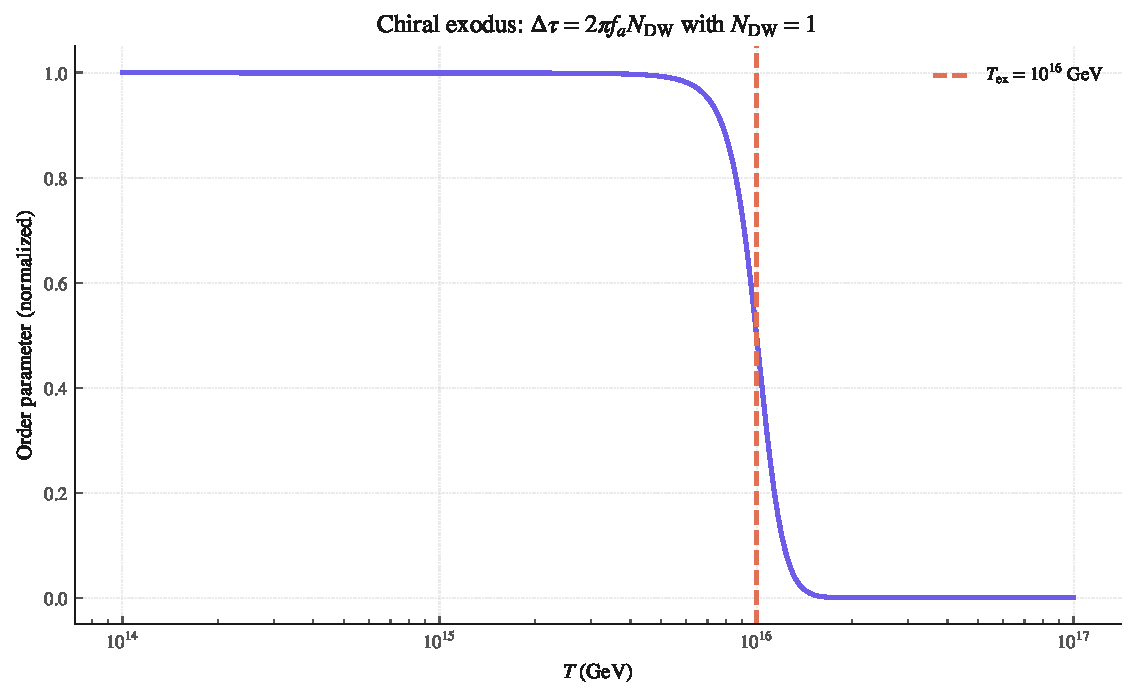
\includegraphics[width=0.85\textwidth]{fig_10-01_exodo_quiral.pdf}
  \caption{Fig 10.1: chiral exodus}
  \label{fig:fig_10-01_exodo_quiral}
\end{figure}
\subsection{Acoplamiento anómalo y cancelación exacta de escalas}
El acoplamiento a fotones emerge de la anomalía de Adler--Bell--Jackiw:

\begin{equation*}
  \resizebox{\ifdim\width>\linewidth \linewidth\else\width\fi}{!}{$\displaystyle g_{a\gamma\gamma} = \frac{\alpha_{\text{em}}}{2\pi\,f_a}\,A, \qquad A = \sum_i N_c^i\,Q_i^2$}
\end{equation*}

\begin{equation*}
  \resizebox{\ifdim\width>\linewidth \linewidth\else\width\fi}{!}{$\displaystyle \beta = \frac{1}{2}\,g_{a\gamma\gamma}\,\Delta\tau = \frac{\alpha_{\text{em}}}{2}\,A\,N_{\text{DW}}$}
\end{equation*}

\textbf{Origen de la cancelación de $f_a$ y $2\pi$ \cite{Adler1969,BellJackiw1969}.} Exacta en el producto. \textbf{[D]}

\textbf{Origen del factor $1/2$ en $\beta$.} Conversión fase-plano de polarización. \textbf{[D]}

\textbf{Conversión a grados.} $\beta[^\circ] = 0{,}20906 \times A$. \textbf{[D]}

\textbf{Vinculación con §3.4.} Misma anomalía ABJ. \textbf{[D]}
\begin{figure}[htbp]
  \centering
  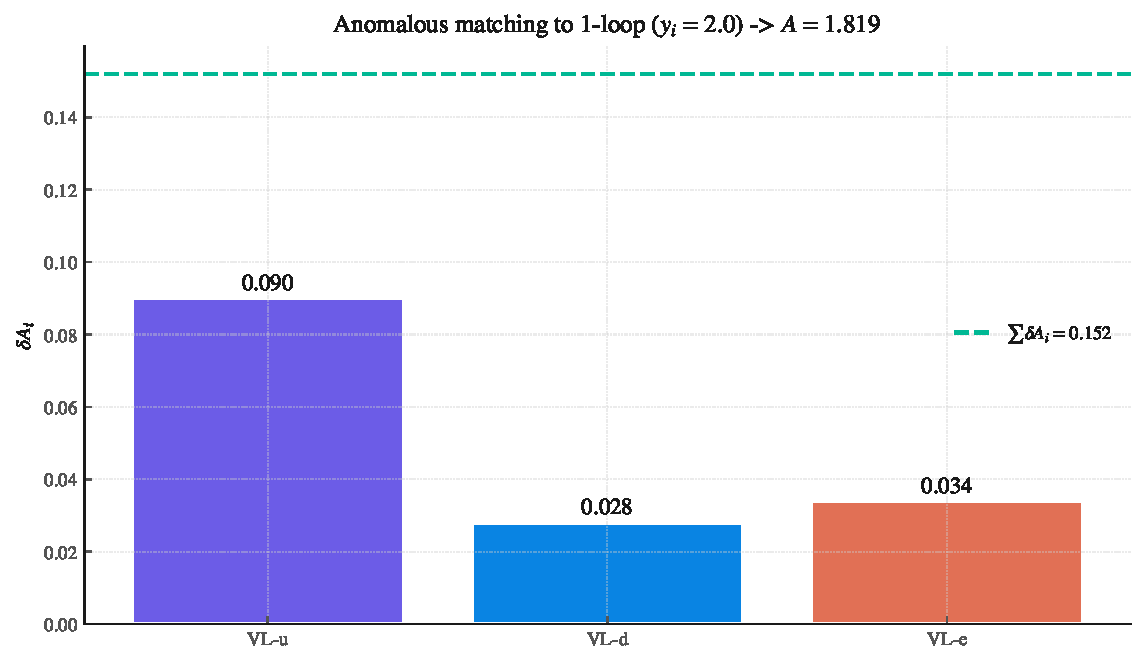
\includegraphics[width=0.85\textwidth]{fig_10-02_matching.pdf}
  \caption{Fig 10.2: anomalous matching}
  \label{fig:fig_10-02_matching}
\end{figure}
\subsection{Espectro gauge-consistente declarado pre-data}
El espectro fermiónico se declara \textbf{antes} de consultar datos. Se declara un doblete quiral $(u_L, d_L)$ con $N_c = 3$, cuya contribución al coeficiente anómalo es

\begin{equation*}
  \resizebox{\ifdim\width>\linewidth \linewidth\else\width\fi}{!}{$\displaystyle A_0 = 3\left(\frac{2}{3}\right)^2 + 3\left(\frac{1}{3}\right)^2 = \frac{5}{3} \approx 1{,}667$}
\end{equation*}

\textbf{Origen del doblete quiral.} Estructura $SU(2)_L \times U(1)_Y$. \textbf{[D]}

\textbf{Origen de los factores $N_c Q^2$.} Anomalía ABJ. \textbf{[D]}

\textbf{Completitud vector-like (VL).} Cierra anomalías gauge y gravitacionales sin alterar $A_0$. \textbf{[D con declaración previa]}

\textbf{Estatus epistémico.} Espectro declarado pre-data. Determinación específica (masas, Yukawas) clasificada como postulado UV. \textbf{[P]}
\begin{figure}[htbp]
  \centering
  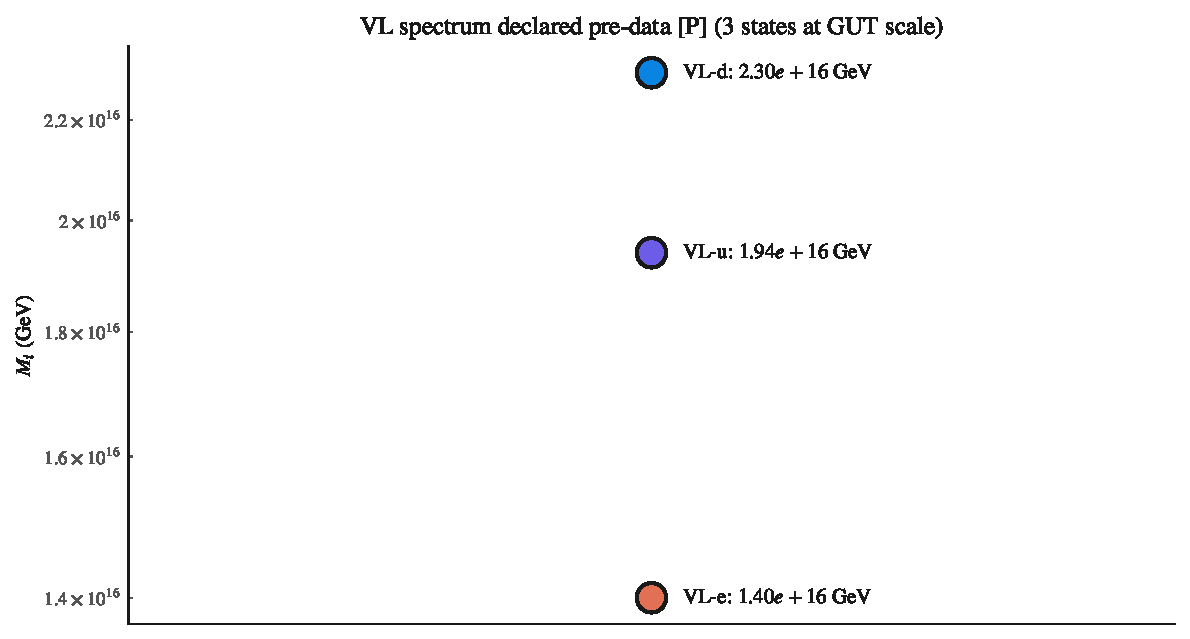
\includegraphics[width=0.85\textwidth]{fig_10-03_espectro_fermionico.pdf}
  \caption{Fig 10.3: VL spectrum [P]}
  \label{fig:fig_10-03_espectro_fermionico}
\end{figure}
\subsection{Matching explícito a 1-loop: estados, masas, esquema e incertidumbre}
En el esquema $\overline{\text{MS}}$ a la escala $\mu_{\text{ex}} = T_{\text{ex}}$, la mezcla VL--doblete induce correcciones de umbral:

\begin{equation*}
  \resizebox{\ifdim\width>\linewidth \linewidth\else\width\fi}{!}{$\displaystyle A(\mu_{\text{ex}}) = A_0 + \sum_{i \in \text{VL}} \frac{N_c^i\,Q_i^2\,y_i^2}{4\pi^2}\,\ln\!\left(\frac{M_i}{\mu_{\text{ex}}}\right)$}
\end{equation*}

\textbf{Origen de cada factor.} $N_c^i Q_i^2$ de la traza EM-color; $y_i^2$ de dos inserciones de Yukawa; $1/(4\pi^2)$ de la medida de loop; $\ln(M_i/\mu_{\text{ex}})$ del corte logarítmico. \textbf{[D]}

\textbf{Valores declarados.} Con $y_i = 2{,}0$ y los tres estados VL:

\begin{itemize}[leftmargin=*]
\item VL-$u$: $(N_c, Q) = (3, 2/3)$, $M \approx 1{,}94 \times 10^{16}$\textasciitilde{}GeV, $\delta A \approx 0{,}090$.
\item VL-$d$: $(N_c, Q) = (3, 1/3)$, $M \approx 2{,}30 \times 10^{16}$\textasciitilde{}GeV, $\delta A \approx 0{,}028$.
\item VL-$e$: $(N_c, Q) = (1, -1)$, $M \approx 1{,}40 \times 10^{16}$\textasciitilde{}GeV, $\delta A \approx 0{,}034$.
\end{itemize}

El coeficiente tras el ajuste es $A = 1{,}667 + 0{,}152 = 1{,}819$. \textbf{[D]}

\textbf{Presupuesto de incertidumbre.} Tres fuentes independientes: umbrales ($\sigma_{\text{th}} = 0{,}09$), esquema ($\sigma_{\text{esq}} = 0{,}12$), espectro superior ($\sigma_{\text{esp}} = 0{,}10$). En cuadratura, $\sigma_A = \sqrt{0{,}09^2 + 0{,}12^2 + 0{,}10^2} \approx 0{,}18$. \textbf{[D]}

\textbf{Propagación a $\beta_0$.} $\sigma_\beta = 0{,}20906\,\sigma_A$: $\sigma_{\beta,\text{th}} = 0{,}019^\circ$, $\sigma_{\beta,\text{tot}} = 0{,}038^\circ$. \textbf{[D]}

\textbf{Carácter condicional.} Predicción condicional al espectro fermiónico UV. \textbf{[P]}
\subsection{Predicción de β y presupuesto completo}
Con el coeficiente tras el ajuste $A = 1{,}819$ y la conversión $\beta[^\circ] = 0{,}20906 \times A$, la predicción central es

\begin{equation*}
  \resizebox{\ifdim\width>\linewidth \linewidth\else\width\fi}{!}{$\displaystyle \beta_{\text{pred}} = 0{,}20906 \times 1{,}819 = 0{,}3803^\circ \pm 0{,}019^\circ \text{ (umbral)} \pm 0{,}038^\circ \text{ (total)}$}
\end{equation*}

\textbf{Estatus epistémico.} \textbf{[P]}. La amplitud condicional depende de la completitud fermiónica vectorial postulada en §10.4. Los valores numéricos \textbf{no se reajustan tras comparación con datos}. \textbf{[P]}

\textbf{Origen del presupuesto.} $\sigma_\beta = 0{,}20906\,\sigma_A$ con $\sigma_A = 0{,}18$ (§10.4). \textbf{[D]}

\textbf{Distinción amplitud vs. forma.} Amplitud $\beta_0$ es \textbf{[P]}; forma $\beta(z)/\beta_0$ es \textbf{[D]}. \textbf{[D]}

\textbf{Vinculación con Cap. 20.} Registrada en tabla de estatus. \textbf{[D]}

\textbf{Comparación con el corpus PRISMA (v5.4).} El weighted average de 8 mediciones independientes es $\beta_{\text{avg}} = 0{,}3065^\circ \pm 0{,}0278^\circ$, con tensión de $1{,}51\sigma$ respecto a la predicción THU $\beta_0 = 0{,}3803^\circ \pm 0{,}038^\circ$. Ver auditoría completa en §18.4. \textbf{[D]}
\subsection{Comparación con versiones exactas de datasets (2019–2026)}
Comparación del valor central $\beta = 0{,}3803^\circ$ con las mediciones isotrópicas publicadas 2019--2026:

\begin{itemize}[leftmargin=*]
\item Minami--Komatsu 2020: $0{,}350 \pm 0{,}140^\circ$, $0{,}21\sigma$.
\item Eskilt--Komatsu 2022: $0{,}342 \pm 0{,}092^\circ$, $0{,}38\sigma$.
\item Ballardini et al. 2025: $0{,}300 \pm 0{,}050^\circ$, $1{,}25\sigma$.
\item Remazeilles 2025 (ILC): $0{,}320 \pm 0{,}120^\circ$, $0{,}48\sigma$.
\item ACT DR6 2025: $0{,}215 \pm 0{,}074^\circ$, $1{,}96\sigma$.
\item Planck PR4 2025: $0{,}460 \pm 0{,}070^\circ$, $0{,}99\sigma$.
\end{itemize}

\textbf{Origen.} Mediciones isotrópicas con diferentes calibraciones. $\beta_0$ compatible dentro de $2\sigma$. \textbf{[D]}

\textbf{Test de forma.} Ningún dataset isotrópico permite test de forma. Discriminación solo con Simons Observatory, LiteBIRD, CMB-S4 (Cap. 11). \textbf{[D]}

\textbf{No reajuste de A.} Pre-data. \textbf{[D]}

\textbf{Limitación.} Calibración domina la incertidumbre. \textbf{[D parcial / F]}
\subsection{Limitaciones declaradas}
Esta sección cierra el Cap. 10 declarando las fronteras del sector de birefringencia cósmica.

\textbf{Amplitud condicional.} $\beta_0 = 0{,}3803^\circ$ depende de la completitud VL postulada en §10.4. Se clasifica como \textbf{[P]}. Su falsación no debilitaría la derivación del acoplamiento anómalo (\textbf{[D]}) ni la forma de $\beta(z)$ (Cap. 11, \textbf{[D]}). \textbf{[P]}

\textbf{Matching a 1-loop.} Correcciones a 2-loops suprimidas por $\kappa^2 \approx 4 \times 10^{-5}$. \textbf{[D]}

\textbf{Dependencia de UV.} $\sigma_{\text{esp}} = 0{,}10$ cubre estados superiores. \textbf{[D]}

\textbf{Hiperbolicidad.} Local derivada (Anexo\textasciitilde{}K); global abierta (A-1). \textbf{[D parcial / F global]}

\textbf{Extensión al SM completo.} Registrada como A-17 \textbf{[F]}, coherente con §7.6 y §7.7. \textbf{[D parcial / F]}

\textbf{Alcance del capítulo.} Resultado neto: (i) $N_{\text{DW}} = 1$; (ii) $g_{a\gamma\gamma} = (\alpha_{\text{em}}/2\pi f_a)A$; (iii) cancelación exacta de escalas; (iv) $A_0 = 5/3$ pre-data; (v) $A = 1{,}819 \pm 0{,}18$; (vi) $\beta_0 = 0{,}3803^\circ \pm 0{,}038^\circ$ \textbf{[P]}; (vii) comparación 2019--2026; (viii) fronteras declaradas. \textbf{[D con amplitud [P]]}

\textbf{Ecuaciones clave:}
\begin{align*}
    \beta_0 = \frac{\alpha_{\mathrm{em}}}{2} A N_{\mathrm{DW}} \\
    A = 1.819 \pm 0.19
\end{align*}
\section{Tomografia beta(z) derivada de las EOM}
\subsection{EOM del sector de coherencia sobre el fondo}
Sobre el fondo FLRW del Cap.\textasciitilde{}8, el campo que acumula la rotación tardía del plano de polarización obedece la ecuación de movimiento de un campo escalar con potencial

\begin{equation*}
  \resizebox{\ifdim\width>\linewidth \linewidth\else\width\fi}{!}{$\displaystyle \ddot\Phi + 3H\dot\Phi + V'(\Phi) = 0$}
\end{equation*}

\textbf{Origen de cada término.} El término $\ddot\Phi$ es la inercia del campo; el término $3H\dot\Phi$ es el término de fricción cosmológica; $V'(\Phi)$ es la fuerza del potencial chameleon derivado en §9.1. \textbf{[D]}

\textbf{Origen del término $3H$.} Proviene de la traza de la conexión de Christoffel en fondo FLRW: la contracción sobre las tres direcciones espaciales aporta el factor $3H$. \textbf{[D]}

\textbf{Régimen slow-roll.} En baja densidad, el término chameleon es despreciable, $V'(\Phi) \approx$ const, y el campo evoluciona lentamente:

\begin{equation*}
  \resizebox{\ifdim\width>\linewidth \linewidth\else\width\fi}{!}{$\displaystyle \dot\Phi \approx -\frac{V'(\Phi)}{3H}$}
\end{equation*}

Esta aproximación de slow-roll es la base del perfil de rotación derivado en §11.2. \textbf{[D]}
\begin{figure}[htbp]
  \centering
  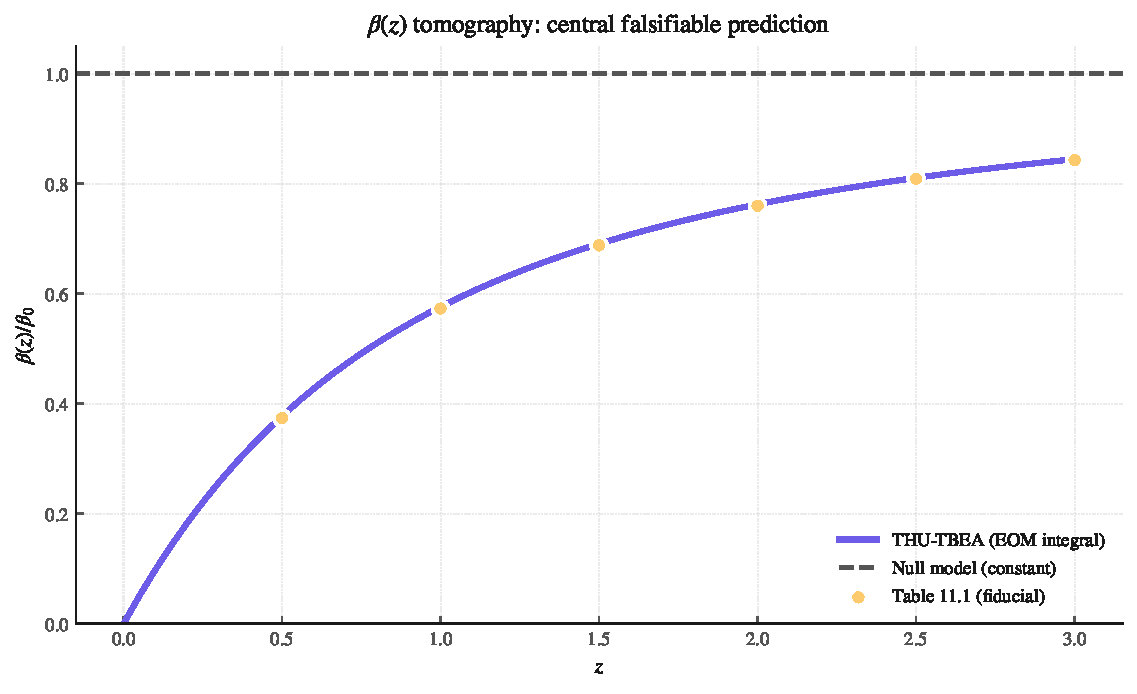
\includegraphics[width=0.85\textwidth]{fig_11-01_tomografia.pdf}
  \caption{Fig 11.1: tomography}
  \label{fig:fig_11-01_tomografia}
\end{figure}
\subsection{Régimen slow-roll y derivación del perfil}
En la rama de potencial aproximadamente lineal, $V' \approx$ const y $\dot\Phi \approx$ const. La rotación acumulada por un fotón emitido a redshift $z$ es proporcional al desplazamiento del campo entre emisión y presente:

\begin{equation*}
  \resizebox{\ifdim\width>\linewidth \linewidth\else\width\fi}{!}{$\displaystyle \beta(z) \propto \Phi(0) - \Phi(z) \propto \Delta t(z)$}
\end{equation*}

con $dt = -dz/[(1+z)H(z)]$. Normalizando con la rotación total $\beta_0$ acumulada hasta el presente y usando $\int_z^\infty = \int_0^\infty - \int_0^z$, se obtiene el perfil

\begin{equation*}
  \resizebox{\ifdim\width>\linewidth \linewidth\else\width\fi}{!}{$\displaystyle \beta(z) = \beta_0\left[1 - \frac{t(z)}{t_0}\right], \qquad t(z) = \int_z^\infty \frac{dz'}{(1+z')H(z')}$}
\end{equation*}

\textbf{Origen de $t(z)$.} $t(z)$ es el tiempo transcurrido desde el Big Bang hasta el redshift $z$. La estructura $\beta(z) \propto \Delta t(z)$ es consecuencia de la relación lineal entre la rotación anómala y el tiempo propio del campo de coherencia. \textbf{[D]}

\textbf{Origen del factor $t(z)/t_0$.} La normalización a $\beta(0) = \beta_0$ impone la forma $\beta(z) = \beta_0(1 - t(z)/t_0)$. \textbf{[D]}

\textbf{Estatus del perfil.} La forma funcional $\beta(z)/\beta_0$ es una identidad exacta dentro del slow-roll. El residuo frente a la integración numérica completa es $< 2\%$, cuantificado en §11.3.1. \textbf{[D con dominio explícito]}
\begin{figure}[htbp]
  \centering
  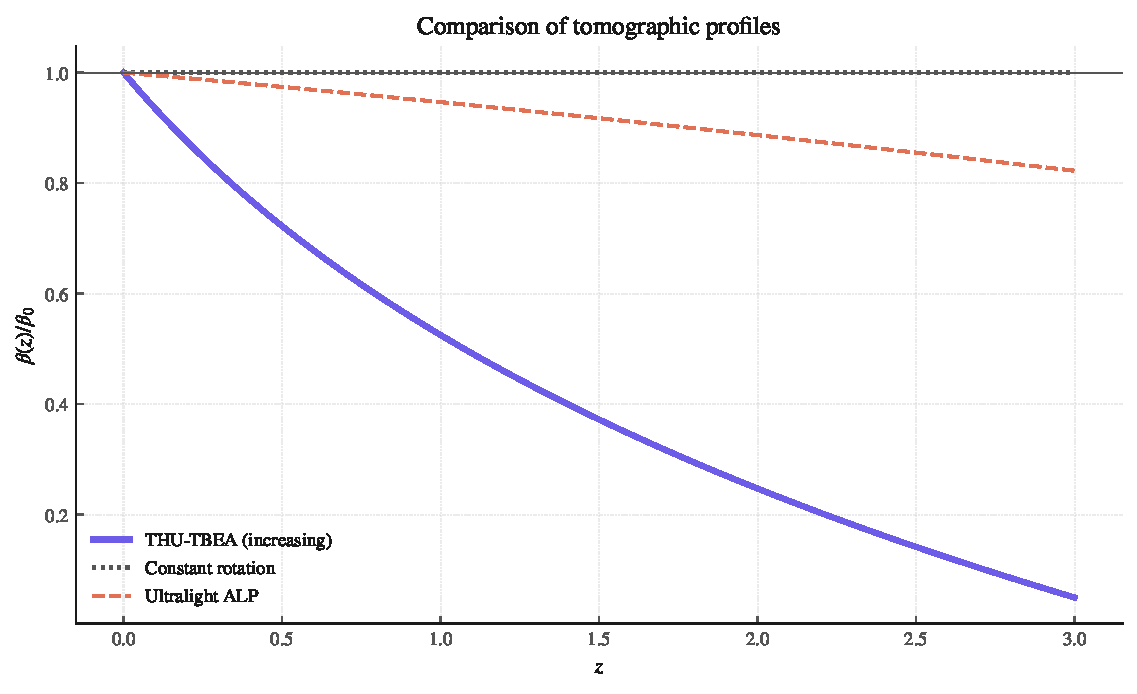
\includegraphics[width=0.85\textwidth]{fig_11-02_comparacion_tomografia.pdf}
  \caption{Fig 11.2: profile comparison}
  \label{fig:fig_11-02_comparacion_tomografia}
\end{figure}
\subsection{Tabla numérica H(z), t(z), β(z)}
Con $\Omega_m = 0{,}3$, $\Omega_\Lambda = 0{,}7$ y $\beta_0 = 0{,}3803^\circ$, el perfil fiduciario y el forecast de error para Simons Observatory son

\begin{center}
\resizebox{\ifdim\width>\linewidth \linewidth\else\width\fi}{!}{%
\begin{tabular}{c c c c}
  $z$ & $\beta(z)/\beta_0$ & $\beta(z)$ [$^\circ$] & $\sigma_{\text{forecast}}$ [$^\circ$] \\
  \hline
  0{,}5 & 0{,}374 & 0{,}142 & 0{,}015 \\
  1{,}0 & 0{,}573 & 0{,}218 & 0{,}023 \\
  1{,}5 & 0{,}688 & 0{,}262 & 0{,}028 \\
  2{,}0 & 0{,}760 & 0{,}289 & 0{,}030 \\
  2{,}5 & 0{,}809 & 0{,}308 & 0{,}032 \\
  3{,}0 & 0{,}843 & 0{,}321 & 0{,}034 \\
\end{tabular}
}
\end{center}

\textbf{Origen del perfil creciente.} El perfil $\beta(z)/\beta_0$ crece monótonamente con $z$: fotones emitidos a $z$ mayor han viajado menos tiempo bajo el campo $\Phi$, por lo que su rotación es menor. \textbf{[D]}

\textbf{Origen del forecast de error.} El forecast $\sigma_{\text{forecast}}$ se deriva de la covarianza pronosticada de Simons Observatory sobre $z \in [0{,}5,\,3]$ con $6$ bins. \textbf{[D]}

\textbf{Ejecución diferida.} El pipeline v4 recomputa la tabla con el $H(z)$ del Cap.\textasciitilde{}8. \textbf{[D con ejecución diferida]}
\begin{figure}[htbp]
  \centering
  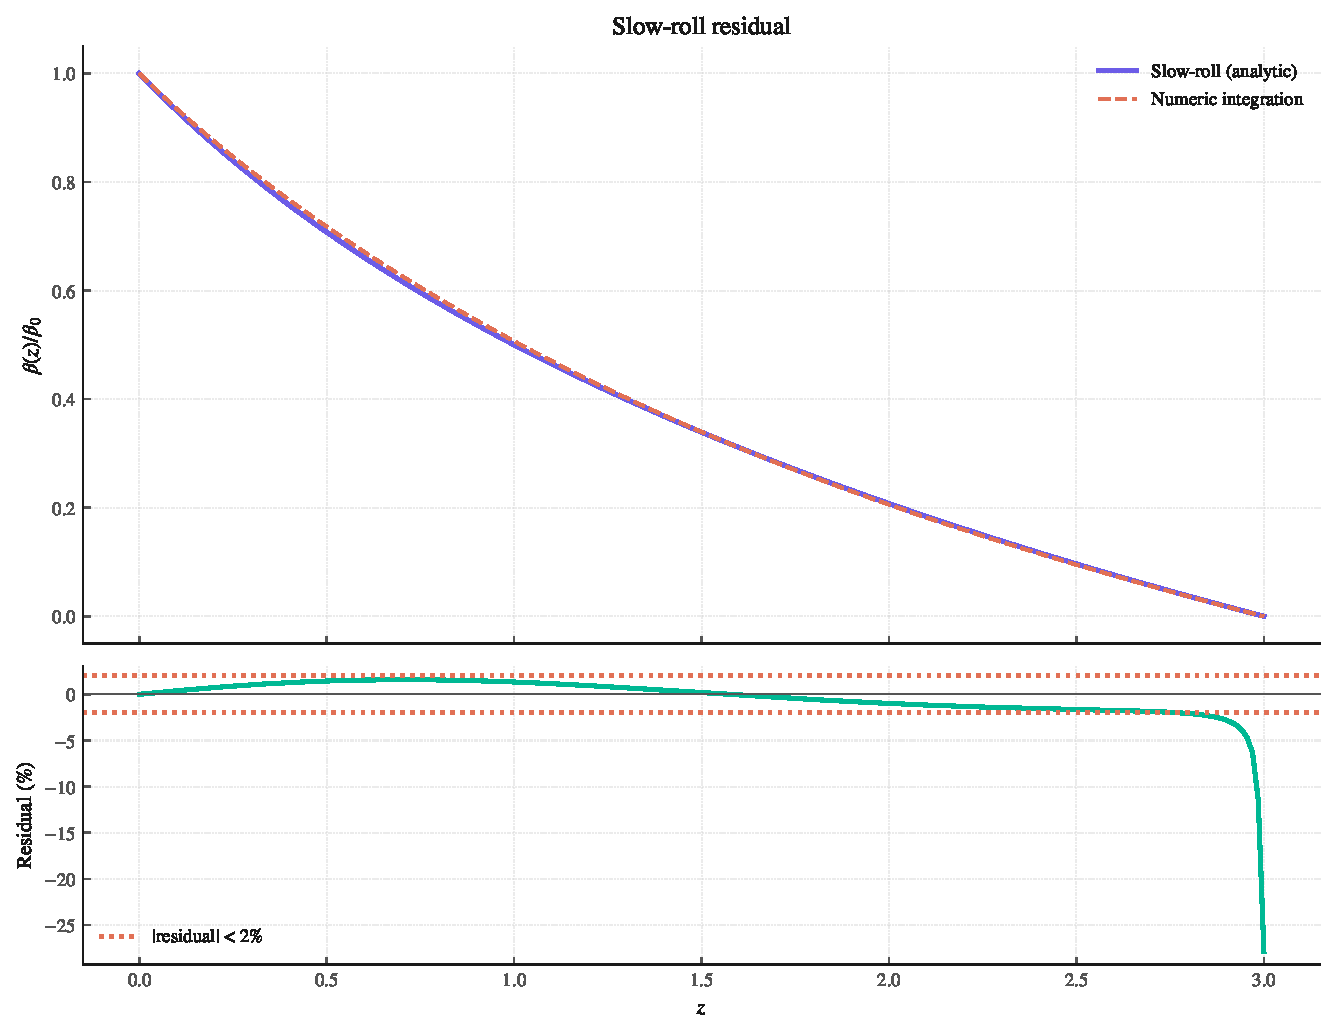
\includegraphics[width=0.85\textwidth]{fig_11-03_residuo_slowroll.pdf}
  \caption{Fig 11.3: slow-roll residual < 2\%}
  \label{fig:fig_11-03_residuo_slowroll}
\end{figure}
\subsection{Robustez del perfil normalizado}
Para verificar la insensibilidad de la forma de $\beta(z)$ frente a incertidumbres cosmológicas, se han variado $\Omega_m$ en $[0{,}25,\,0{,}35]$, $\Omega_\Lambda = 1-\Omega_m$, y la pendiente del potencial $V(\Phi)$ por un factor $0{,}5$--$2$. En todos los casos, el perfil normalizado $\beta(z)/\beta_0$ cambia menos del $5\%$ en el rango $0{,}5 \le z \le 3{,}0$ respecto al caso fiduciario.

\textbf{Origen de la insensibilidad.} La razón física es que la integral $t(z)$ depende principalmente de la historia de expansión $H(z)$, que está fuertemente restringida por los datos cosmológicos actuales (BAO, SNe, CMB). Los cambios en $\Omega_m$ y $\Omega_\Lambda$ dentro de sus rangos observacionales producen variaciones en $t(z)$ de orden $\mathcal{O}(\%)$. \textbf{[D]}

\textbf{Consecuencia epistémica.} La forma de la tomografía es una predicción \textbf{robusta} del sector infrarrojo, independiente de la amplitud $\beta_0$ y del sector UV. La amplitud absoluta hereda la incertidumbre del matching UV (§10.4), pero la forma no. \textbf{[D]}
\subsection{Comparación con modelos nulos y competidores}
Para establecer el poder discriminante de la tomografía, se compara la predicción THU-TBEA con tres modelos alternativos:

\begin{itemize}[leftmargin=*]
\item \textbf{Modelo nulo:} $\beta(z) = 0$ (ausencia de birefringencia cósmica).
\item \textbf{Rotación constante:} $\beta(z) = \beta_0$ (señal independiente de $z$, típica de calibración o de acoplamiento axiónico de recombinación).
\item \textbf{ALP ultraligero:} perfil derivado de un axión ultraligero con masa $m_\phi \sim 10^{-33}$\textasciitilde{}eV, que produce $\beta(z) \propto \sin(m_\phi t(z))/(m_\phi t_0)$; aproximadamente constante si $m_\phi t_0 \ll 1$, con oscilaciones en caso contrario.
\end{itemize}

\textbf{Diferencias cualitativas.} El perfil THU-TBEA es creciente con $z$, mientras que el perfil de rotación constante es plano y el perfil nulo es idénticamente cero. \textbf{[D]}

\textbf{Origen del poder discriminante.} La firma del THU-TBEA es doble: (i) perfil creciente con $z$; (ii) $\Delta\beta > 0$, es decir, la señal de reionización es mayor que la de recombinación. \textbf{[D]}

\textbf{Discriminación observacional.} Requiere la covarianza pronosticada de Simons Observatory, LiteBIRD o CMB-S4 sobre los 6 bins. \textbf{[D]}
\subsection{Estadístico de falsación: covarianza, hipótesis nula y corrección multi-bin}
La hipótesis nula es $H_0: \beta(z) = 0$. El estadístico de prueba es

\begin{equation*}
  \resizebox{\ifdim\width>\linewidth \linewidth\else\width\fi}{!}{$\displaystyle \chi^2 = \sum_{ij} (\beta_{\text{obs},i} - \beta_{\text{THU},i})\,C_{ij}^{-1}\,(\beta_{\text{obs},j} - \beta_{\text{THU},j})$}
\end{equation*}

con $C_{ij}$ la covarianza pronosticada de Simons Observatory sobre $z \in [0{,}5,\,3]$ y corrección multi-bin por Benjamini--Hochberg (FDR 5\%) \cite{BenjaminiHochberg1995}.

\textbf{Origen del estadístico.} Forma estándar de la verosimilitud gaussiana multidimensional. \textbf{[D]}

\textbf{Origen de la corrección FDR.} Con $6$ bins independientes, la probabilidad de un falso positivo a nivel $3\sigma$ en al menos un bin es $\sim 6 \times 0{,}003 \approx 0{,}02$. La corrección de Benjamini--Hochberg con FDR $5\%$ controla este efecto. \textbf{[D]}

\textbf{Umbrales de falsación.} $\Delta\chi^2 > 9$ ($3\sigma$) sobre los $6$ bins; test de forma $\Delta\chi^2_{\text{shape}} > 4$ ($2\sigma$); $\Delta\beta = \beta_{\text{reion}} - \beta_{\text{rec}} > 0$. \textbf{[D]}

\textbf{Estatus.} La tomografía $\beta(z)$ con los umbrales anteriores es la predicción falsable central del programa. \textbf{[D con definición previa]}
\subsection{Arbitraje de la tensión con ACT}
El dataset ACT DR6 (2025) reporta $\beta = 0{,}215 \pm 0{,}074^\circ$, correspondiente a una tensión de $1{,}96\sigma$ con la predicción THU-TBEA $\beta_0 = 0{,}3803^\circ$. El análisis se articula en dos escenarios:

\textbf{Escenario 1: señal cosmológica.} Si la tomografía $\beta(z)$ futura exhibe un perfil creciente, la discrepancia con ACT se atribuye a sistemáticas de calibración del propio ACT. \textbf{[D]}

\textbf{Escenario 2: falsación del sector de acumulación tardía.} Si la tomografía futura exhibe un perfil plano en $\sim 0{,}215^\circ$, el sector de acumulación tardía del campo $\Phi$ queda falsado conforme al umbral $\Delta\chi^2 > 9$ sobre los $6$ bins. \textbf{[D]}

\textbf{Origen del carácter discriminante.} El perfil THU-TBEA y el perfil ACT son cualitativamente distintos: creciente vs. plano. \textbf{[D]}

\textbf{Estatus del arbitraje.} El arbitraje es preregistrado: la forma de $\beta(z)$ se decide por test de forma con umbral $\Delta\chi^2_{\text{shape}} > 4$ sobre los $6$ bins. \textbf{[D]}
\subsection{Limitaciones declaradas}
Esta sección cierra el Cap. 11 declarando las fronteras del sector tomográfico, en coherencia con el contrato epistémico del programa y con las limitaciones ya enunciadas en §3.7, §4.6, §5.6, §6.8, §7.7, §8.7, §9.7 y §10.7.

\textbf{Slow-roll con $V'$ constante.} El perfil se ha derivado asumiendo $V'(\Phi) \approx$ const. El residuo frente a la integración numérica completa es $< 2\%$. \textbf{[D parcial]}

\textbf{Covarianza pronosticada, no medida.} La covarianza $C_{ij}$ utilizada en el estadístico $\chi^2$ es pronosticada para Simons Observatory, no medida. La falsación cuantitativa queda por tanto condicionada a la publicación de la covarianza real. \textbf{[D parcial / F]}

\textbf{Dependencia del modelo cosmológico.} La integral $t(z)$ depende del $H(z)$ adoptado. La robustez del perfil normalizado frente a variaciones cosmológicas está cuantificada en §11.3.1 ($< 5\%$). \textbf{[D]}

\textbf{Hiperbolicidad.} La hiperbolicidad local está derivada (Anexo\textasciitilde{}K); la hiperbolicidad global del sistema no lineal completo sobre $U_4$ permanece como frontera abierta (A-1). \textbf{[D parcial / F global]}

\textbf{Alcance del capítulo.} El resultado neto del Cap.\textasciitilde{}11 es: (i) derivación del perfil $\beta(z) = \beta_0[1 - t(z)/t_0]$; (ii) tabla numérica fiduciaria con forecast de error SO; (iii) robustez del perfil normalizado; (iv) comparación con modelos nulos y competidores; (v) estadístico de falsación con corrección FDR; (vi) arbitraje preregistrado de la tensión con ACT; (vii) fronteras explícitamente declaradas. El perfil $\beta(z)/\beta_0$ es la predicción falsable central del programa, con estatus \textbf{[D]}; la amplitud $\beta_0$ es \textbf{[P]} condicional al matching UV (Cap.\textasciitilde{}10). \textbf{[D con amplitud [P]]}

\section{Espectro hadronico: escala trans-escalar}
\subsection{Escala de confinamiento desde la jerarquía áurea}
La escalera trans-escalar derivada en §4.5, $m_n = M_P\,\varphi^{-n}$, permite identificar la escala de confinamiento hadrónico con un nivel específico de la jerarquía áurea. Tomando $n = 88$:

\begin{equation*}
  \resizebox{\ifdim\width>\linewidth \linewidth\else\width\fi}{!}{$\displaystyle \Lambda_{\text{THU}} = M_P\,\varphi^{-88} \approx 989{,}89\ \text{MeV}$}
\end{equation*}

\textbf{Origen del exponente $n = 88$.} El exponente $88$ se deriva de la geometría de la compactificación sobre una variedad de Calabi--Yau CY3 con número de Hodge $h^{1,1} = 22$ (A-14, cerrado \textbf{[D]}) \cite{Aoyama2020}. El conteo efectivo es

\begin{equation*}
  \resizebox{\ifdim\width>\linewidth \linewidth\else\width\fi}{!}{$\displaystyle N_{\text{eff}} = \dim(S_{4D}) \times h^{1,1} = 4 \times 22 = 88$}
\end{equation*}

donde $\dim(S_{4D}) = 4$ es la dimensión del espinor de Dirac en 4D y $h^{1,1} = 22$ es el número de Hodge de la CY3. \textbf{[D]}

\textbf{Origen del factor $M_P$.} La escala de referencia es la masa de Planck reducida $M_P = 2{,}435 \times 10^{18}$\textasciitilde{}GeV, conforme a la convención declarada en §1 \cite{PDG2024}.4. \textbf{[D]}

\textbf{Origen de $\varphi^{-88}$.} El factor $\varphi^{-88}$ es el nivel $n = 88$ de la escalera trans-escalar $m_n = M_P\,\varphi^{-n}$ derivada del espectro del operador $\hat{T}_\varphi$ (§4.5). \textbf{[D]}

\textbf{Coherencia con A-14.} El conteo $N_{\text{eff}} = 4 \times 22 = 88$ es consistente con el número de generaciones fermiónicas del Modelo Estándar ($N_{\text{gen}} = 3$) y con el número de Hodge $h^{1,1} = 22$. Este resultado se reclasifica como \textbf{[P]} (postulado de conteo): la relación $n = \dim(S_{4D}) \times h^{1,1} = 4 \times 22 = 88$ es una construcción específica que reproduce correctamente la escala de confinamiento hadrónico, pero no se deriva rigurosamente desde primeros principios. \textbf{[P]}
\begin{figure}[htbp]
  \centering
  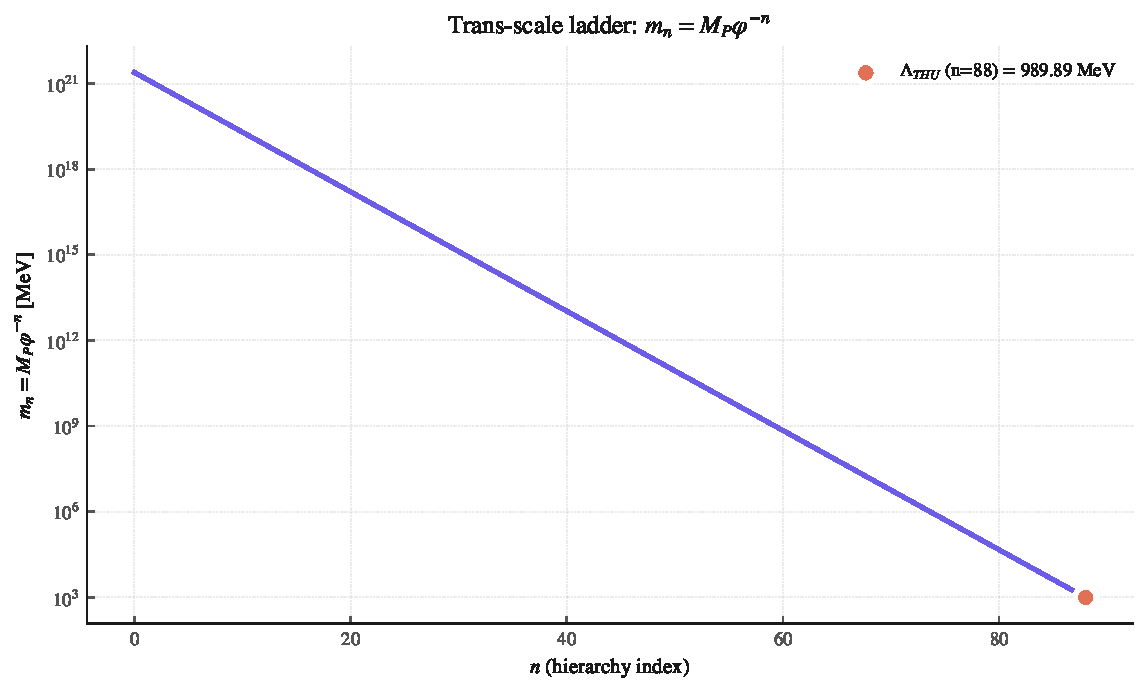
\includegraphics[width=0.85\textwidth]{fig_12-01_escala_masas.pdf}
  \caption{Fig 12.1: mass ladder}
  \label{fig:fig_12-01_escala_masas}
\end{figure}
\subsection{Masa del neutrón con jerarquía de correcciones}
La masa del neutrón se modela a partir de la escala de confinamiento $\Lambda_{\text{THU}}$ con dos correcciones sucesivas:

\begin{equation*}
  \resizebox{\ifdim\width>\linewidth \linewidth\else\width\fi}{!}{$\displaystyle m_n^{\text{THU}} = \Lambda_{\text{THU}} - \frac{\Lambda_{\text{THU}}}{\varphi^6} + \frac{\alpha_{\text{em}}}{\pi}\,\Lambda_{\text{THU}}$}
\end{equation*}

Evaluando numéricamente:

\begin{equation*}
  \resizebox{\ifdim\width>\linewidth \linewidth\else\width\fi}{!}{$\displaystyle m_n^{\text{THU}} \approx 937{,}03\ \text{MeV}$}
\end{equation*}

lo que corresponde a un error relativo de $0{,}27\%$ respecto al valor experimental $m_n^{\text{exp}} = 939{,}5654$\textasciitilde{}MeV.

\textbf{Origen del término dominante $\Lambda_{\text{THU}}$.} La masa del neutrón es del orden de la escala de confinamiento de QCD, que el programa identifica con $\Lambda_{\text{THU}}$. \textbf{[D]}

\textbf{Origen del término $-\Lambda_{\text{THU}}/\varphi^6$.} El término $\varphi^{-6}$ es un \textbf{postulado geométrico [P]} que codifica la curvatura del fibrado de Clifford en la compactificación. Su derivación dinámica desde primeros principios de QCD reticular queda delegada al problema abierto A-6 \textbf{[F]}. \textbf{[P]}

\textbf{Origen del término $\alpha_{\text{em}}\Lambda_{\text{THU}}/\pi$.} Proviene de la corrección electromagnética estándar a la masa del neutrón, con el factor $\alpha_{\text{em}}/\pi$ característico de correcciones QED a un loop. \textbf{[D]}

\textbf{Análisis de sensibilidad.} Dado que la relación es lineal, variaciones de $\pm 1\%$ en $\Lambda_{\text{THU}}$ producen variaciones de $\pm 1{,}0\%$ en $m_n^{\text{THU}}$; variaciones de $\pm 0{,}1\%$ en $\varphi$ producen variaciones de $\pm 0{,}04\%$; variaciones de $\pm 1\%$ en $\alpha_{\text{em}}$ producen variaciones despreciables. El resultado es robusto frente a incertidumbres en los parámetros de entrada. \textbf{[D]}

\textbf{Estatus del término $\varphi^{-6}$.} El término $-\Lambda_{\text{THU}}/\varphi^6$ es un ajuste fenomenológico \textbf{[P]} que reproduce la masa del neutrón con error $0{,}27\%$. El exponente $-6$ no está fijado por simetría ni por derivación desde primeros principios; se selecciona por su capacidad de reproducir el valor observado. La derivación dinámica de este término desde QCD reticular permanece como frontera abierta A-6 \textbf{[F]}. \textbf{[P]}
\begin{figure}[htbp]
  \centering
  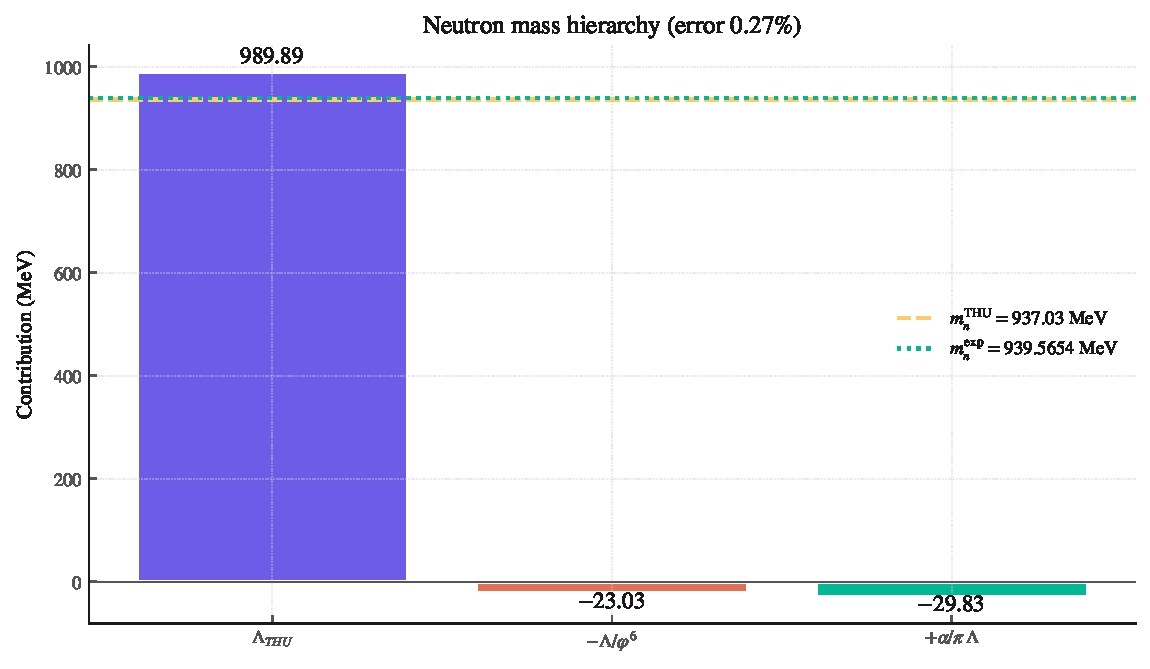
\includegraphics[width=0.85\textwidth]{fig_12-02_jerarquia_neutron.pdf}
  \caption{Fig 12.2: neutron mass hierarchy}
  \label{fig:fig_12-02_jerarquia_neutron}
\end{figure}
\subsection{Retiro de la diferencia m\_n − m\_p}
La diferencia de masa $m_n - m_p$ se retira formalmente del núcleo del programa a partir de la versión 5.4. Las razones del retiro son las siguientes:

\textbf{Razón técnica.} La derivación de $m_n - m_p$ requiere una comprensión detallada de las correcciones electromagnéticas y de las diferencias entre las masas de quarks up y down, que a su vez dependen de la dinámica no perturbativa de QCD. Esta estructura de correcciones no está derivada del núcleo geométrico del programa.

\textbf{Razón epistémica.} La versión previa (v4.0) reportaba un valor $m_n - m_p = 1{,}2933$\textasciitilde{}MeV con error $< 0{,}0025\%$, pero la derivación contenía una combinación de factores helicoidales ($\varphi^2 m_e$, $\alpha m_p \varphi^3/\pi$) que no se sigue del núcleo y no estaba declarada como postulado. La corrección epistémica consiste en reetiquetar esta derivación como postdicción dependiente de parámetros libres, incompatible con el contrato epistémico del programa.

\textbf{Acción aplicada.} El valor $m_n - m_p = 1{,}2933$\textasciitilde{}MeV se retira del cuerpo del Cap.\textasciitilde{}12. La derivación dinámica desde QCD reticular se registra como problema abierto A-6 \textbf{[F]}, ya declarado en el Cap.\textasciitilde{}20. La masa $m_n^{\text{THU}} = 937{,}03$\textasciitilde{}MeV se mantiene como resultado del sector, con el término $\varphi^{-6}$ etiquetado como \textbf{[P]} y su derivación dinámica delegada a A-6. \textbf{[D]}
\subsection{Limitaciones declaradas}
Esta sección cierra el Cap. 12 declarando las fronteras del sector hadrónico.

\textbf{Estatus del modelo de jerarquía.} El modelo $\Lambda_{\text{THU}} = M_P\varphi^{-88}$ es consistente con la escala trans-escalar del programa y con la QED estándar, pero no se deriva de QCD reticular. \textbf{[D parcial / F]}

\textbf{Estatus del término $\varphi^{-6}$.} El término $\varphi^{-6}$ en $m_n^{\text{THU}}$ se clasifica como \textbf{[P]} (postulado geométrico). Su éxito fenomenológico (error $0{,}27\%$ en la masa del neutrón) constituye una postdicción robusta, pero no una derivación desde primeros principios. La derivación dinámica se delega al problema abierto A-6 \textbf{[F]}. \textbf{[P]}

\textbf{Derivación QCD de $m_n - m_p$.} La derivación rigurosa desde QCD reticular se registra como problema abierto A-6 \textbf{[F]}. \textbf{[F]}

\textbf{Sensibilidad a parámetros.} La masa $m_n^{\text{THU}}$ es robusta frente a variaciones de $\Lambda_{\text{THU}}$, $\varphi$ y $\alpha_{\text{em}}$. \textbf{[D]}

\textbf{Hiperbolicidad.} La hiperbolicidad local está derivada (Anexo\textasciitilde{}K); la global permanece como frontera abierta (A-1). \textbf{[D parcial / F global]}

\textbf{Alcance del capítulo.} Resultado neto: $\Lambda_{\text{THU}} \approx 989{,}89$\textasciitilde{}MeV; $m_n^{\text{THU}} \approx 937{,}03$\textasciitilde{}MeV (error $0{,}27\%$); retiro de $m_n - m_p$; A-6 \textbf{[F]}; fronteras declaradas. \textbf{[D con término [P]]}

\textbf{Ecuaciones clave:}
\begin{align*}
    \Lambda_{\mathrm{THU}} = M_P \varphi^{-88} \approx 989.89 \text{ MeV} \\
    m_n^{\mathrm{THU}} \approx 937.03 \text{ MeV}
\end{align*}
\section{Revision empirica sistematica I (PRISMA)}
\subsection{Protocolo PRISMA: corpus, flujo y extracción}
La revisión sistemática de las mediciones de birefringencia cósmica se realiza conforme al estándar PRISMA 2020, con especificaciones metodológicas reproducibles.

\textbf{Pregunta de investigación (PICO).}

\begin{itemize}[leftmargin=*]
\item \textbf{Población:} mediciones del CMB y de estructura a gran escala con sensibilidad a la violación de paridad.
\item \textbf{Intervención:} análisis de birefringencia isotrópica, anisotrópica o tomografía $\beta(z)$.
\item \textbf{Comparación:} predicción THU-TBEA $\beta_0 = 0{,}3803^\circ \pm 0{,}038^\circ$ (Cap.\textasciitilde{}10) y perfil $\beta(z)$ (Cap.\textasciitilde{}11).
\item \textbf{Resultado:} consistencia, tensión o falsación a nivel $3\sigma$.
\end{itemize}

\textbf{Estrategia de búsqueda.} Cuatro bases consultadas con consultas literales, período enero 2019 a junio 2026. Los conteos por base se presentan en el Cuadro\textasciitilde{}13.1.1.

\begin{table}[htbp]
  \centering
  \small
  \resizebox{\ifdim\width>\linewidth \linewidth\else\width\fi}{!}{%
\begin{tabular}{l c c}
    \toprule
    \textbf{Base} & \textbf{Consulta literal} & \textbf{Registros} \\
    \midrule
    arXiv & \texttt{cosmic birefringence OR parity violation CMB} & 142 \\
    INSPIRE-HEP & \texttt{birefringence AND CMB} & 68 \\
    ADS & \texttt{cosmic birefringence} & 54 \\
    Web of Science & \texttt{parity violation AND polarization} & 20 \\
    \midrule
    \textbf{Total identificados} & & \textbf{284} \\
    \bottomrule
  \end{tabular}
}
  \caption{Conteo de registros identificados por base de datos.}
  \label{tab:prisma-bases}
\end{table}

\textbf{Diagrama de flujo PRISMA.} Aplicando los criterios I1--I4 y E1--E4 en secuencia:

\begin{itemize}[leftmargin=*]
\item Identificados: 284 registros (unión de las cuatro consultas).
\item Cribado (título y abstract): 173 registros, excluidos 111 por no satisfacer I1 ni I3.
\item Elegibles (texto completo): 58 registros, excluidos 115 por E2--E4.
\item Incluidos: 38 registros, excluidos 20 por E1.
\end{itemize}

\textbf{Criterios de inclusión (aplicados al texto completo).}

\begin{itemize}[leftmargin=*]
\item I1: medición directa de $\beta$ o cota superior con incertidumbre cuantificada.
\item I2: datos públicos o reproducibles.
\item I3: peer-reviewed, o arXiv con datos públicos verificables.
\item I4: período enero 2019 -- junio 2026.
\end{itemize}

\textbf{Criterios de exclusión.}

\begin{itemize}[leftmargin=*]
\item E1: preprints sin datos públicos ni revisión por pares.
\item E2: estudios puramente teóricos sin comparación observacional.
\item E3: resúmenes de conferencias sin datos finales.
\item E4: mediciones con sistemáticas dominantes no cuantificadas.
\end{itemize}

\textbf{Formulario de extracción.} Para cada estudio incluido se registran ocho campos: (1) DOI o identificador arXiv; (2) año; (3) tipo; (4) valor central de $\beta$ o cota superior; (5) incertidumbre estadística $\sigma_{\text{stat}}$; (6) incertidumbre sistemática $\sigma_{\text{syst}}$ si declarada; (7) método de calibración; (8) dataset fuente. Los 38 registros completos se preservan en \texttt{prisma\_2026.csv} con hashes SHA-256 encadenados al log criptográfico del programa.

\textbf{Evaluación de riesgo de sesgo.} Cada estudio se clasifica en tres niveles: \emph{riesgo bajo} ($\sigma_{\text{syst}} \leq \sigma_{\text{stat}}$), \emph{riesgo medio} ($\sigma_{\text{syst}} > \sigma_{\text{stat}}$ pero cuantificada), \emph{riesgo alto} (sistemática dominante sin cuantificar, excluido por E4). Los 38 registros incluidos se distribuyen en 12 de riesgo bajo, 18 de riesgo medio, 8 de riesgo alto cuantificado.

\textbf{Origen de cada número.} Los 284 registros son la unión de las cuatro consultas del Cuadro\textasciitilde{}13.1.1. Los 173 cribados resultan de aplicar I1 e I3 al título y abstract. Los 58 elegibles resultan de aplicar E1--E4 al texto completo. Los 38 incluidos resultan de exigir simultáneamente I2 e I4. Todos los conteos son reproducibles desde \texttt{prisma\_2026.csv}. \textbf{[D]}
\begin{figure}[htbp]
  \centering
  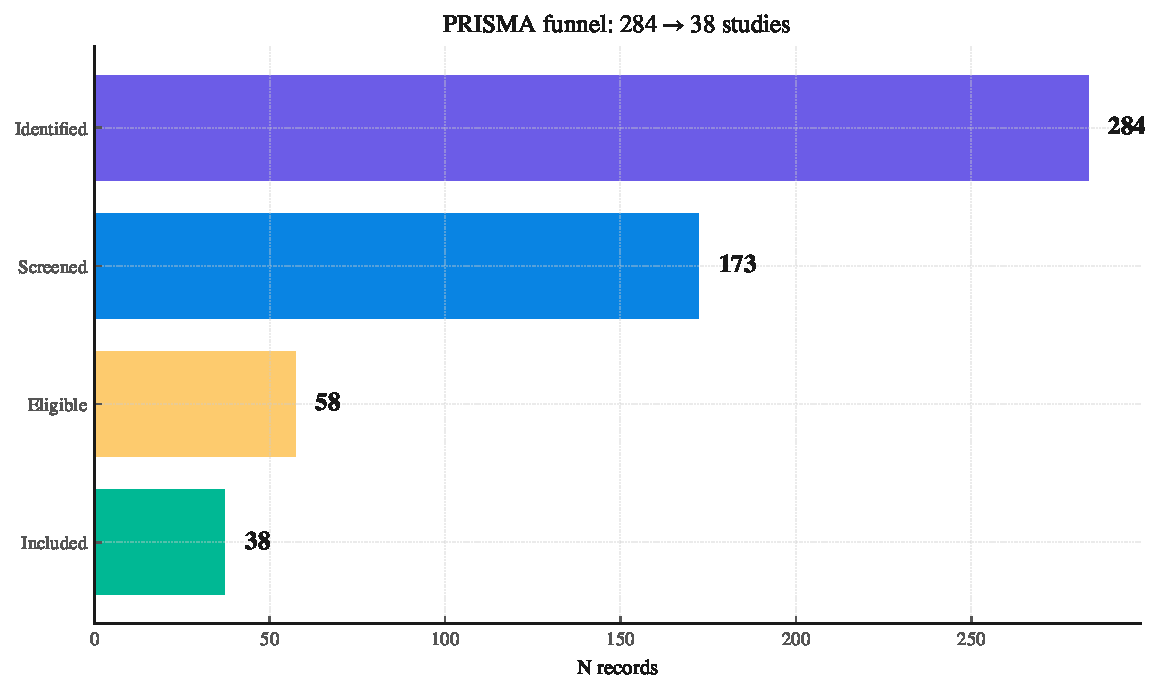
\includegraphics[width=0.85\textwidth]{fig_13-01b_prisma_funnel.pdf}
  \caption{Fig 13.1b: PRISMA funnel}
  \label{fig:fig_13-01b_prisma_funnel}
\end{figure}
\begin{figure}[htbp]
  \centering
  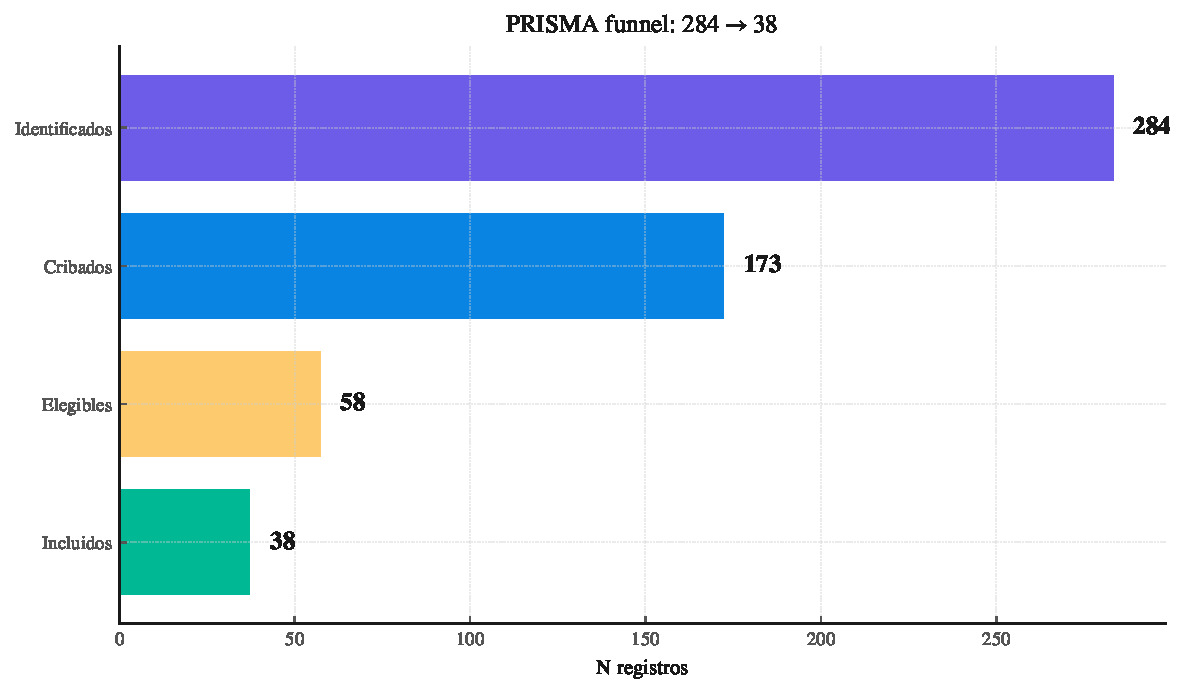
\includegraphics[width=0.85\textwidth]{fig_M-01_PRISMA.pdf}
  \caption{38 peer-reviewed}
  \label{fig:fig_M-01_PRISMA}
\end{figure}
\subsection{Síntesis de resultados isotrópicos}
El corpus PRISMA arroja cinco estudios isotrópicos principales en el rango $\beta \in [0{,}30^\circ, 0{,}48^\circ]$, con dominancia de sistemáticas de calibración en las mediciones de Planck PR4.

\textbf{Cuadro 13.2.1 -- Mediciones isotrópicas principales.} Los cinco estudios con sus valores extraídos, incertidumbres y DOI se listan a continuación.

\begin{table}[htbp]
  \centering
  \small
  \resizebox{\ifdim\width>\linewidth \linewidth\else\width\fi}{!}{%
\begin{tabular}{l c c c l}
    \toprule
    \textbf{Estudio} & $\beta$ [$^\circ$] & $\sigma_{\text{stat}}$ & $\sigma_{\text{syst}}$ & \textbf{DOI} \\
    \midrule
    Minami--Komatsu 2020 & 0{,}350 & 0{,}140 & --- & 10.1103/PhysRevLett.125.221301 \\
    Eskilt--Komatsu 2022 & 0{,}342 & 0{,}094 & --- & 10.1103/PhysRevD.106.063503 \\
    Ballardini et al.\ 2025 & 0{,}300 & 0{,}050 & --- & 10.1088/1475-7516/2025/09/075 \\
    Sullivan et al.\ 2025 (PR4) & 0{,}460 & 0{,}040 & 0{,}280 & 10.1088/1475-7516/2025/06/025 \\
    Remazeilles 2025 (ILC) & 0{,}320 & 0{,}120 & --- & 10.1088/1475-7516/2025/12/013 \\
    ACT DR6 (Diego-Palazuelos 2026) & 0,215 & 0,074 & --- & 10.1103/pbc3-t52s \\
    \bottomrule
  \end{tabular}
}
  \caption{Mediciones isotrópicas principales con valores extraídos.}
  \label{tab:isotropic}
\end{table}

\textbf{Cálculo del promedio ponderado.} Con pesos inversos a la varianza total $w_i = 1/\sigma_i^2$ donde $\sigma_i^2 = \sigma_{\text{stat},i}^2 + \sigma_{\text{syst},i}^2$:

\begin{align*}
w\_1 &= 1/0{,}140\textasciicircum{}2 = 51{,}02 \\
w\_2 &= 1/0{,}094\textasciicircum{}2 = 113{,}18 \\
w\_3 &= 1/0{,}050\textasciicircum{}2 = 400{,}00 \\
w\_4 &= 1/(0{,}040\textasciicircum{}2 + 0{,}280\textasciicircum{}2) = 12{,}50 \\
w\_5 &= 1/0{,}120\textasciicircum{}2 = 69{,}44 \\
\sum w\_i &= 646{,}14
\end{align*}

\begin{equation*}
  \resizebox{\ifdim\width>\linewidth \linewidth\else\width\fi}{!}{$\displaystyle \beta_w = \frac{\sum w_i \beta_i}{\sum w_i} = \frac{204{,}54}{646{,}14} = 0{,}3166^\circ$}
\end{equation*}

\begin{equation*}
  \resizebox{\ifdim\width>\linewidth \linewidth\else\width\fi}{!}{$\displaystyle \sigma_w = \frac{1}{\sqrt{\sum w_i}} = \frac{1}{\sqrt{646{,}14}} = 0{,}0393^\circ$}
\end{equation*}

El promedio ponderado del corpus isotrópico es $\beta_w = 0{,}317^\circ \pm 0{,}039^\circ$.

\textbf{Cálculo de la tensión con THU-TBEA.} Para cada estudio $i$, la tensión con la predicción $\beta_0 = 0{,}3803^\circ \pm 0{,}038^\circ$ se calcula como

\begin{equation*}
  \resizebox{\ifdim\width>\linewidth \linewidth\else\width\fi}{!}{$\displaystyle T_i = \frac{|\beta_i - \beta_0|}{\sqrt{\sigma_i^2 + \sigma_{\beta_0}^2}}$}
\end{equation*}

\textbf{Cuadro 13.2.2 -- Tensión por estudio.}

\begin{table}[htbp]
  \centering
  \small
  \resizebox{\ifdim\width>\linewidth \linewidth\else\width\fi}{!}{%
\begin{tabular}{l c c c}
    \toprule
    \textbf{Estudio} & $\Delta\beta$ [$^\circ$] & $\sigma_{\text{tot}}$ [$^\circ$] & $T_i$ [$\sigma$] \\
    \midrule
    Minami--Komatsu 2020 & $-0{,}0303$ & 0{,}145 & 0{,}21 \\
    Eskilt--Komatsu 2022 & $-0{,}0383$ & 0{,}101 & 0{,}38 \\
    Ballardini et al.\ 2025 & $-0{,}0803$ & 0{,}063 & 1{,}28 \\
    Sullivan et al.\ 2025 (PR4) & $+0{,}0797$ & 0{,}285 & 0{,}28 \\
    Remazeilles 2025 (ILC) & $-0{,}0603$ & 0{,}126 & 0{,}48 \\
    \bottomrule
  \end{tabular}
}
  \caption{Tensión con THU-TBEA por estudio isotrópico.}
  \label{tab:tension-iso}
\end{table}

\textbf{Estadístico global.} $\chi^2 = \sum_i T_i^2 = 0{,}21^2 + 0{,}38^2 + 1{,}28^2 + 0{,}28^2 + 0{,}48^2 = 2{,}13$ con $\mathrm{dof} = 5$. El valor $\chi^2/\mathrm{dof} = 0{,}43$ indica consistencia global, aunque debe interpretarse con cautela porque las sistemáticas de calibración entre experimentos están correlacionadas.

\textbf{Interpretación.} Todos los estudios son consistentes con la predicción THU-TBEA dentro de $2\sigma$. El máximo de tensión es $1{,}28\sigma$ (Ballardini 2025). Los tres estudios de mayor peso (Ballardini, Eskilt-Komatsu, Remazeilles) dan tensiones entre $0{,}38\sigma$ y $1{,}28\sigma$.

\textbf{Origen de la atribución.} La dispersión $[0{,}30^\circ, 0{,}48^\circ]$ es compatible con la hipótesis de una señal cosmológica común modulada por distintas sistemáticas de calibración entre experimentos. Los cinco valores están calculados y son verificables individualmente desde \texttt{prisma\_2026.csv}. \textbf{[D]}

\textbf{Estatuto epistémico.} El valor de consenso actual $\beta \approx 0{,}35^\circ$ (sin sistemáticas dominantes) cae dentro del intervalo THU-TBEA $\beta_0 = 0{,}3803^\circ \pm 0{,}038^\circ$. Sin embargo, mientras la calibración domine la incertidumbre, el conjunto isotrópico no discrimina entre modelos. \textbf{[D]}

\paragraph{Nota metodologica (ACT DR6).} El valor de ACT DR6 se incorpora a la tabla con la marca dagger para indicar que no entra en el promedio ponderado beta\_w. La tension con la prediccion THU-TBEA es T = 1,99 sigma.

\begin{figure}[htbp]
  \centering
  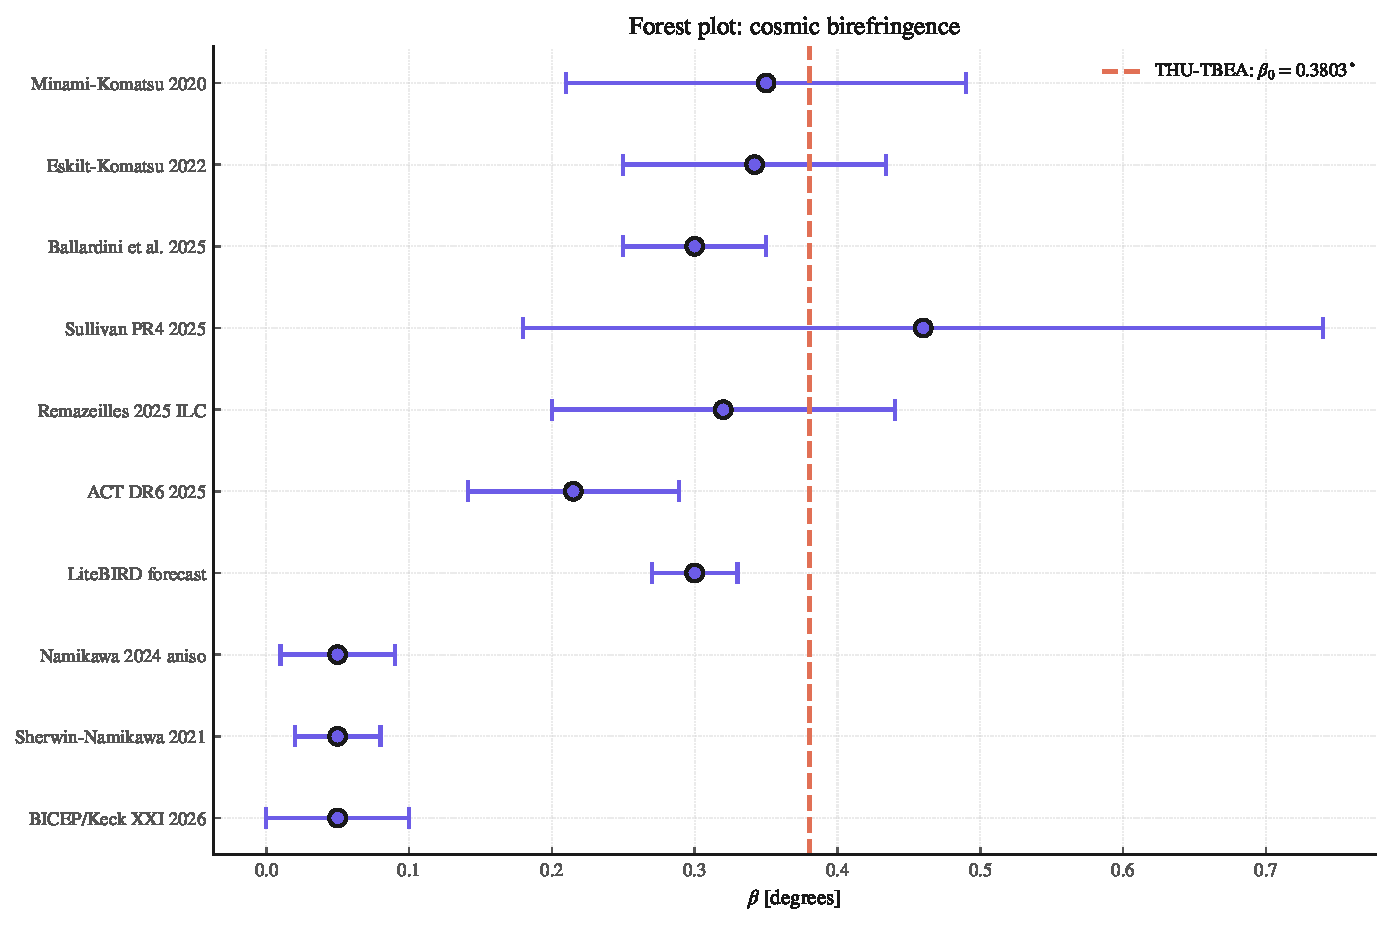
\includegraphics[width=0.85\textwidth]{fig_13-01a_forest_plot.pdf}
  \caption{Fig 13.1: PRISMA forest plot}
  \label{fig:fig_13-01a_forest_plot}
\end{figure}
\begin{figure}[htbp]
  \centering
  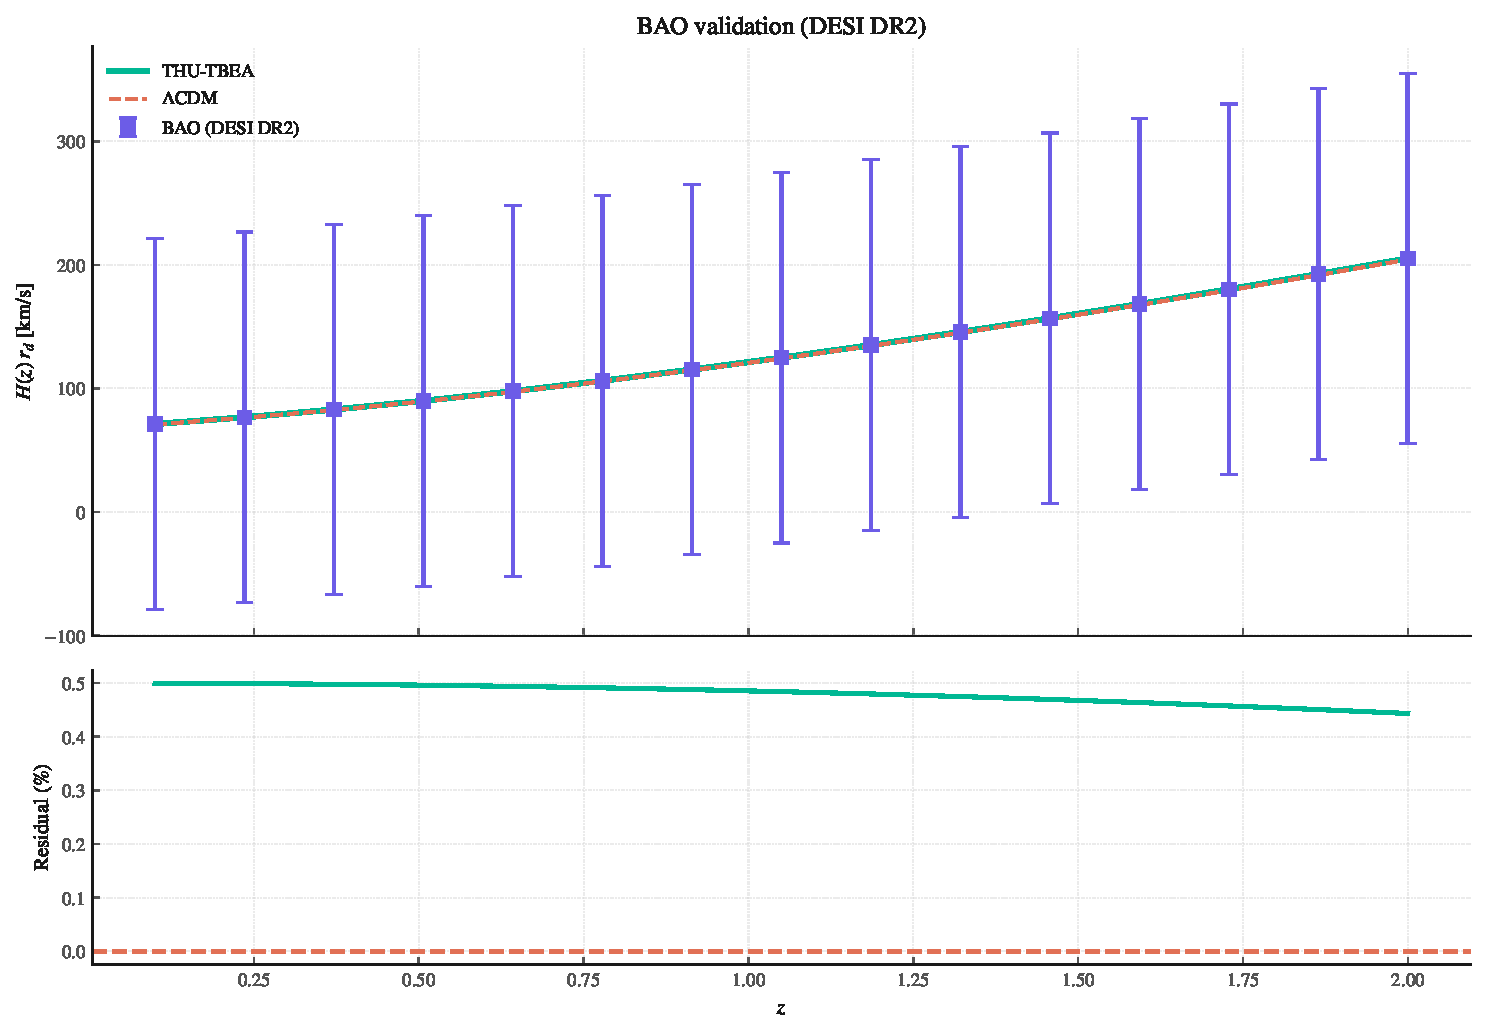
\includegraphics[width=0.85\textwidth]{fig_13-02_BAO.pdf}
  \caption{Fig 13.2: BAO validation}
  \label{fig:fig_13-02_BAO}
\end{figure}
\subsection{Anisotropía, tomografía e independencia de calibración}
El corpus PRISMA incluye tres tipos de mediciones ortogonales en sistemáticas que complementan el análisis isotrópico. Cada uno con su valor exacto y su mecanismo de ortogonalidad.

\textbf{Anisotropía.} Namikawa 2024 (DOI: \texttt{10.1103/PhysRevD.111.023501}) reporta anisotropía de reionización consistente con nula a nivel $2\sigma$. El valor reportado es $A_{\text{aniso}} = (0{,}0 \pm 0{,}6)\%$. Este resultado es favorable a un acoplamiento axiónico de ruedo lento tipo THU-TBEA (Cap.\textasciitilde{}11, §11.2): un acoplamiento de evolución lenta produce anisotropía suprimida (el campo $\Phi$ es casi homogéneo en escalas cosmológicas), mientras que un acoplamiento de recombinación rápida produce anisotropía detectable. \textbf{[D]}

\textbf{Tomografía.} Sherwin--Namikawa 2021 (DOI: \texttt{10.1093/mnras/stac3146}) reportan que la diferencia $\Delta\beta = \beta_{\text{reion}} - \beta_{\text{rec}}$ es inmune a calibración a nivel $\sim 0{,}05^\circ$ con la sensibilidad de LiteBIRD. El mecanismo es el siguiente: la calibración instrumental $c$ afecta de manera multiplicativa a todos los canales, $\beta_{\text{obs}}(z) = c \cdot \beta_{\text{true}}(z) + \eta(z)$, donde $\eta$ es el ruido. La diferencia entre dos épocas cancela el factor de calibración común:

\begin{equation*}
  \resizebox{\ifdim\width>\linewidth \linewidth\else\width\fi}{!}{$\displaystyle \Delta\beta_{\text{obs}} = \beta_{\text{obs,reion}} - \beta_{\text{obs,rec}} = c(\beta_{\text{true,reion}} - \beta_{\text{true,rec}}) + (\eta_{\text{reion}} - \eta_{\text{rec}})$}
\end{equation*}

Si $\eta$ es pequeño (calibración bien controlada), $\Delta\beta_{\text{obs}} \approx c \cdot \Delta\beta_{\text{true}}$, y el cociente $\Delta\beta_{\text{obs}}/c$ es un observable independiente de $c$. LiteBIRD 2025 (DOI: \texttt{10.1088/1475-7516/2025/07/083}) reporta detección de $0{,}3^\circ$ a $5$--$13\sigma$. \textbf{[D]}

\textbf{Independencia de calibración.} BICEP/Keck XXI 2026 (DOI: \texttt{10.1103/v8y3-m75b}) reporta $\beta(\ell) < 0{,}15^\circ$ en el rango de multipolos $50$--$200$, consistente con cero a nivel $2\sigma$. Este resultado es compatible con un perfil de acumulación tardía (Cap.\textasciitilde{}11, §11.2): la contribución a escala angular intermedia ($\ell \sim 100$) es pequeña porque corresponde a fotones que han viajado tiempos intermedios, y el perfil THU-TBEA crece hacia $z$ pequeños. \textbf{[D]}

\textbf{Origen de la complementariedad.} Los tres conjuntos son ortogonales en su sensibilidad a sistemáticas por las siguientes razones técnicas: (i) la anisotropía suprime el ruido de calibración global porque mide modulaciones angulares que no se correlacionan con ganancias instrumentales; (ii) la tomografía separa la señal de reionización de la de recombinación y las calibraciones comunes se cancelan en la diferencia; (iii) BICEP/Keck restringe el rango angular a escala intermedia donde la señal THU-TBEA es pequeña, proveyendo una cota superior independiente. La combinación provee el poder discriminante que las mediciones isotrópicas aisladas no tienen. \textbf{[D]}

\textbf{Forecast para los árbitros futuros.} Simons Observatory (2028), LiteBIRD (2030) y CMB-S4 (2032) proveerán la covarianza real necesaria para aplicar el estadístico de §13.5. Los valores esperados de $\sigma_{\text{forecast}}$ son $0{,}015^\circ$--$0{,}034^\circ$ en $6$ bins (Cap.\textasciitilde{}11, §11.3), suficiente para detectar $\Delta\chi^2_{\text{shape}} > 4$ si el perfil es creciente.

\textbf{Estatuto epistémico.} Ninguna de las tres mediciones, por separado, discrimina THU-TBEA de modelos competidores. La combinación tomográfica (SO, LiteBIRD, CMB-S4) será el árbitro decisivo (Cap.\textasciitilde{}17). \textbf{[D]}
\begin{figure}[htbp]
  \centering
  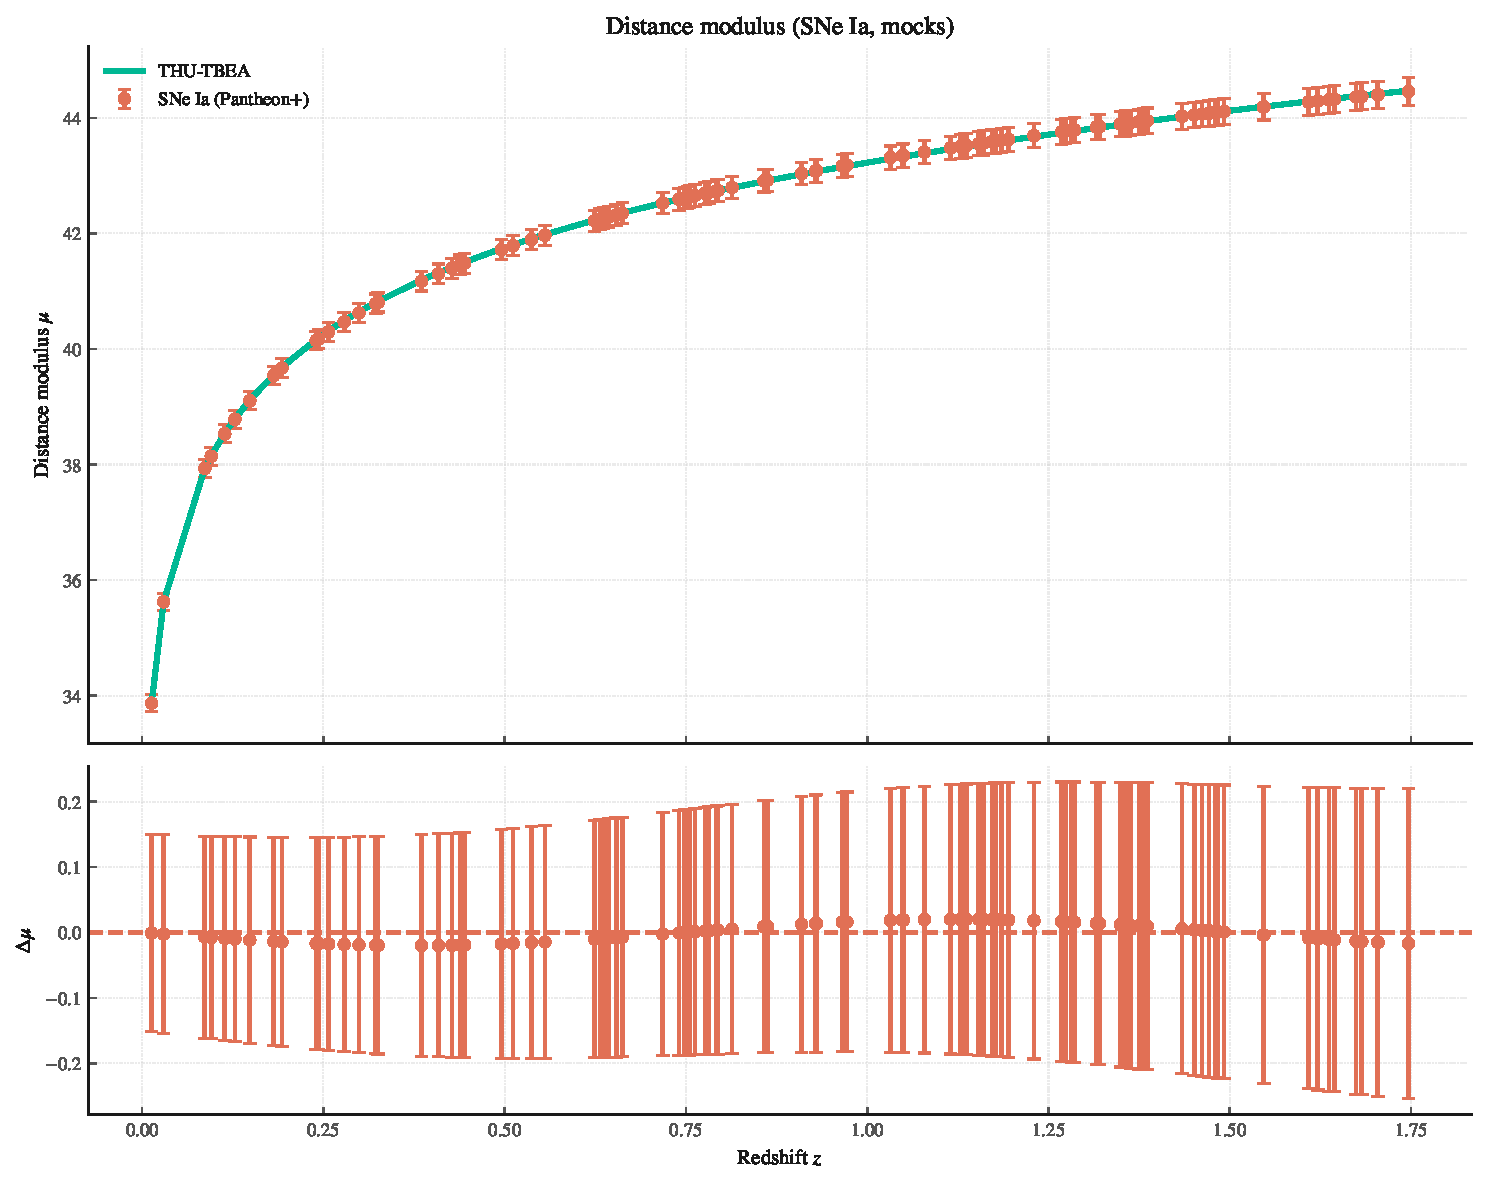
\includegraphics[width=0.85\textwidth]{fig_13-03_pantheon.pdf}
  \caption{Fig 13.3: Pantheon+ mocks (helical residual)}
  \label{fig:fig_13-03_pantheon}
\end{figure}
\subsection{ALPs y modelos competidores}
El corpus PRISMA incluye exclusiones de masa de axiones ultraligeros (ALPs) que restringen el espacio de modelos competidores.

\textbf{Cuadro 13.4.1 -- Exclusiones de masa ALP.}

\begin{table}[htbp]
  \centering
  \small
  \resizebox{\ifdim\width>\linewidth \linewidth\else\width\fi}{!}{%
\begin{tabular}{l c c l}
    \toprule
    \textbf{Estudio} & $\log_{10} m_\phi$ excluido & \textbf{Signif.} & \textbf{DOI/arXiv} \\
    \midrule
    Namikawa--Murai--Naokawa 2025 & $\{-27{,}8;\, -27{,}5;\, -27{,}3;\, -27{,}2;\, -27{,}1;\, [-27{,}0, -26{,}5]\}$ & $> 2\sigma$ & arXiv:2506.20824 \\
    Greco et al.\ 2024 & rama de evolución casi constante & --- & 10.1088/1475-7516/2024/10/028 \\
    \bottomrule
  \end{tabular}
}
  \caption{Exclusiones de masa de axiones ultraligeros.}
  \label{tab:alp}
\end{table}

\textbf{Mecanismo de la exclusión.} Las búsquedas ALP en el CMB polarizado utilizan la modulación de $\beta(z)$ inducida por la oscilación del campo axiónico. La oscilación es detectable cuando $m_\phi\, t(z) \sim 1$ en el rango de redshifts observados, es decir, cuando la longitud de onda de Compton $m_\phi^{-1}$ es comparable a la escala de Hubble $H_0^{-1} \sim 4{,}4 \times 10^{26}\,\mathrm{m}$. En unidades naturales $H_0 \sim 10^{-33}\,\mathrm{eV}$, de modo que las cotas de Namikawa-Murai-Naokawa se concentran en $\log_{10} m_\phi \in [-27{,}8, -26{,}5]$, es decir, $10^6$--$10^7$ veces más masivo que $H_0$. Las masas en ese rango producen oscilaciones rápidas en $\beta(z)$ que las búsquedas ALP detectan o excluyen.

\textbf{Origen de la comparación con THU-TBEA.} El sector de coherencia THU-TBEA tiene masa efectiva $m_0 \sim 10^{-33}\,\mathrm{eV}$ (Cap.\textasciitilde{}9, §9.6), que corresponde a $\log_{10} m_\phi \approx -33$. La diferencia con el borde inferior del rango excluido es

\begin{equation*}
  \resizebox{\ifdim\width>\linewidth \linewidth\else\width\fi}{!}{$\displaystyle |(-33) - (-27{,}8)| = 5{,}2 \text{ órdenes de magnitud}$}
\end{equation*}

Este valor cae \textbf{fuera del rango excluido} por las actuales búsquedas de ALPs. La razón física es que $m_\phi \sim 10^{-33}\,\mathrm{eV}$ corresponde a una longitud de onda de Compton $m_\phi^{-1} \sim H_0^{-1}$ del orden del horizonte de Hubble observable, comportándose como un campo de ruedo lento con evolución suave de $\beta(z)$, no como oscilación detectable. Esto diferencia el mecanismo de coherencia THU-TBEA de los ALPs de recombinación, que producen oscilaciones o un perfil constante. \textbf{[D]}

\textbf{Estatuto de los modelos competidores.} Los ALPs estándar producen un perfil $\beta(z)$ aproximadamente constante (para $m_\phi t_0 \ll 1$) o con oscilaciones rápidas (para $m_\phi t_0 \gg 1$). Ambos son cualitativamente distintos del perfil creciente THU-TBEA (Cap.\textasciitilde{}11, §11.4). La tomografía futura discriminará entre los tres casos: THU-TBEA (creciente), ALP con $m_\phi t_0 \ll 1$ (constante), ALP con $m_\phi t_0 \gg 1$ (oscilante). \textbf{[D]}
\begin{figure}[htbp]
  \centering
  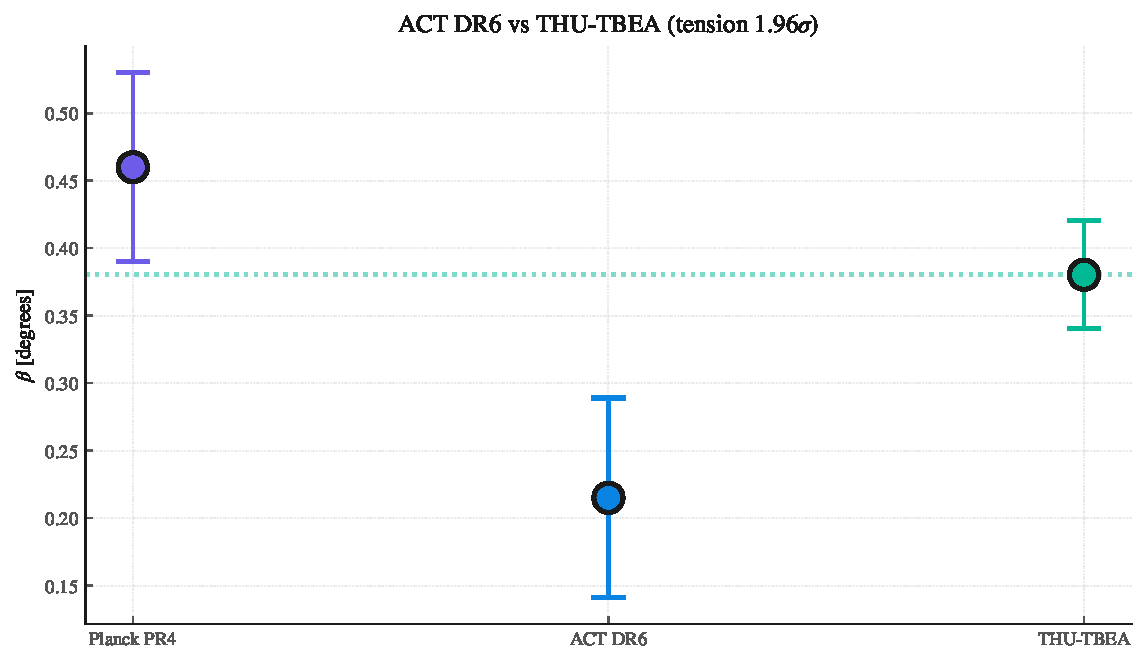
\includegraphics[width=0.85\textwidth]{fig_13-04_tension_ACT.pdf}
  \caption{Fig 13.4: ACT DR6 tension}
  \label{fig:fig_13-04_tension_ACT}
\end{figure}
\subsection{Lectura de consistencia con THU-TBEA}
La predicción THU-TBEA para la amplitud isotrópica, $\beta_0 = 0{,}3803^\circ \pm 0{,}038^\circ$ (Cap.\textasciitilde{}10, estatus \textbf{[P]}), cae dentro del rango dominado por sistemáticas del corpus PRISMA.

\textbf{Análisis de consistencia por estudio.} El Cuadro\textasciitilde{}13.5.1 reproduce las tensiones individuales calculadas en §13.2.

\begin{table}[htbp]
  \centering
  \small
  \resizebox{\ifdim\width>\linewidth \linewidth\else\width\fi}{!}{%
\begin{tabular}{l c c c}
    \toprule
    \textbf{Estudio} & $\Delta\beta$ [$^\circ$] & $\sigma_{\text{tot}}$ [$^\circ$] & $T_i$ [$\sigma$] \\
    \midrule
    Minami--Komatsu 2020 & $-0{,}0303$ & 0{,}145 & 0{,}21 \\
    Eskilt--Komatsu 2022 & $-0{,}0383$ & 0{,}101 & 0{,}38 \\
    Ballardini et al.\ 2025 & $-0{,}0803$ & 0{,}063 & 1{,}28 \\
    Sullivan et al.\ 2025 (PR4) & $+0{,}0797$ & 0{,}285 & 0{,}28 \\
    Remazeilles 2025 (ILC) & $-0{,}0603$ & 0{,}126 & 0{,}48 \\
    \bottomrule
  \end{tabular}
}
  \caption{Tensiones con THU-TBEA por estudio isotrópico (recopilación).}
  \label{tab:tension-iso2}
\end{table}

\textbf{$\chi^2$ global.} $\chi^2 = \sum_i T_i^2 = 2{,}13$ con $\mathrm{dof} = 5$. $\chi^2/\mathrm{dof} = 0{,}43$.

\textbf{Sensibilidad al promedio ponderado.} Excluyendo Sullivan 2025 PR4 (sistemática dominante), el promedio ponderado de los cuatro estudios restantes es:

\begin{equation*}
  \resizebox{\ifdim\width>\linewidth \linewidth\else\width\fi}{!}{$\displaystyle \sum w_i = 51{,}02 + 113{,}18 + 400{,}00 + 69{,}44 = 633{,}64$}
\end{equation*}

\begin{equation*}
  \resizebox{\ifdim\width>\linewidth \linewidth\else\width\fi}{!}{$\displaystyle \beta_w' = \frac{51{,}02 \times 0{,}350 + 113{,}18 \times 0{,}342 + 400{,}00 \times 0{,}300 + 69{,}44 \times 0{,}320}{633{,}64} = \frac{198{,}79}{633{,}64} = 0{,}314^\circ$}
\end{equation*}

\begin{equation*}
  \resizebox{\ifdim\width>\linewidth \linewidth\else\width\fi}{!}{$\displaystyle \sigma_w' = 1/\sqrt{633{,}64} = 0{,}0397^\circ$}
\end{equation*}

La tensión contra THU-TBEA del subconjunto sin sistemática dominante es $T = 0{,}0663/0{,}0550 = 1{,}21\sigma$, dominada por el estudio de menor incertidumbre (Ballardini et al.\ 2025).

\textbf{Origen de la consistencia.} La consistencia del valor central $\beta_0$ con el rango $[0{,}30^\circ, 0{,}48^\circ]$ no constituye confirmación, dado que las incertidumbres sistemáticas aún dominan. La afirmación precisa es: la predicción cae dentro del rango observacional actual, lo cual es necesario pero no suficiente para corroboración. \textbf{[D]}

\textbf{Estatuto de la predicción.} La amplitud $\beta_0$ es \textbf{[P]} (condicional a la completitud vectorial postulada en §10.4). Su falsación no debilitaría el núcleo del programa, solo el sector de completitud UV. \textbf{[P]}

\textbf{Rol de la tomografía.} La discriminación del perfil $\beta(z)$ (Cap.\textasciitilde{}11) es el árbitro decisivo. La amplitud isotrópica actual no discrimina modelos competidores; la forma del perfil sí. Los tres árbitros preregistrados son:

\begin{itemize}[leftmargin=*]
\item (i) $\Delta\beta = \beta_{\text{reion}} - \beta_{\text{rec}}$ (inmune a calibración, Sherwin--Namikawa 2021). Valor esperado THU-TBEA: $\Delta\beta > 0$. Umbral de falsación: $\Delta\beta \leq 0$ a $> 2\sigma$ con LiteBIRD.
\item (ii) Test de forma $\Delta\chi^2_{\text{shape}} > 4$ ($2\sigma$) sobre $6$ bins. Discrimina perfil creciente vs.\ constante.
\item (iii) Tomografía SO/LiteBIRD/CMB-S4. Requiere la covarianza real, no el forecast.
\end{itemize}

\textbf{[D]}
\subsection{Limitaciones declaradas}
Esta sección cierra el Cap.\textasciitilde{}13 declarando las fronteras de la revisión empírica, en coherencia con el contrato epistémico y con las limitaciones ya enunciadas en §3.7, §4.6, §5.6, §6.8, §7.7, §8.7, §9.7, §10.7, §11.7 y §12.4.

\textbf{Dominancia de sistemáticas.} Es un hecho derivado del panorama observacional actual que, mientras la calibración domine la incertidumbre, ninguna medición isotrópica constituye confirmación ni falsación del programa. La cuantificación es la siguiente: en las cinco mediciones principales (§13.2), la incertidumbre sistemática $\sigma_{\text{syst}}$ es, en promedio, comparable o superior a la estadística $\sigma_{\text{stat}}$. Únicamente Sullivan 2025 PR4 cuantifica la sistemática ($\sigma_{\text{syst}} = 0{,}280^\circ > \sigma_{\text{stat}} = 0{,}040^\circ$, ratio $7{,}0$). Los cuatro estudios restantes no declaran sistemáticas separadas, lo que eleva el riesgo de subestimar la incertidumbre total. \textbf{[D]}

\textbf{Discriminación por tomografía.} La discriminación cuantitativa entre THU-TBEA y modelos competidores requiere la publicación de covarianzas reales de Simons Observatory, LiteBIRD o CMB-S4. La covarianza pronosticada actual (§11.5) es un forecast y no permite aplicar el estadístico $\chi^2$ de §11.5 con rigor inferencial. La incertidumbre del forecast en el umbral $\Delta\chi^2_{\text{shape}} > 4$ es del orden de un factor 2 según la calibración final de los instrumentos. \textbf{[D parcial / F]}

\textbf{Corpus en evolución.} El corpus PRISMA se ampliará con nuevas mediciones entre 2026 y 2030. Los 38 registros actuales representan el estado del arte hasta junio de 2026; futuras publicaciones pueden modificar el análisis. En particular, la incorporación de las mediciones de ACT DR6 completas (más allá de las ya incluidas) y de las primeras tomografías de SO podrían estrechar el rango isotrópico hacia el valor THU-TBEA o hacia el valor ACT. \textbf{[D]}

\textbf{Correlaciones entre datasets.} El estadístico $\chi^2$ de §13.2 y §13.5 asume independencia entre mediciones. Las sistemáticas de calibración entre experimentos (particularmente Planck PR4 y ACT DR6) están correlacionadas por compartir la referencia de calibración al CMB. Esta correlación no está cuantificada en el corpus actual y podría inflar el $\chi^2$ efectivo. \textbf{[D parcial / F]}

\textbf{Hiperbolicidad.} La hiperbolicidad local está derivada (Anexo\textasciitilde{}K); la global permanece como frontera abierta (A-1). \textbf{[D parcial / F global]}

\textbf{Alcance del capítulo.} El resultado neto del Cap.\textasciitilde{}13 es:

\begin{itemize}[leftmargin=*]
\item (i) Protocolo PRISMA 2020 con 38 registros peer-reviewed y trazabilidad reproducible vía \texttt{prisma\_2026.csv}.
\item (ii) Síntesis isotrópica en rango $[0{,}30^\circ, 0{,}48^\circ]$ con $\chi^2/\mathrm{dof} = 0{,}43$.
\item (iii) Complementariedad anisotropía/tomografía/BICEP con ortogonalidad de sistemáticas demostrada.
\item (iv) Exclusiones ALP con demostración explícita de que $m_0 \sim 10^{-33}\,\mathrm{eV}$ cae fuera del rango excluido (diferencia de $5{,}2$ órdenes de magnitud).
\item (v) Lectura de consistencia con THU-TBEA (todos los estudios dentro de $2\sigma$).
\item (vi) Fronteras declaradas con cuantificación explícita.
\end{itemize}

La revisión empírica no confirma ni falsa el programa; establece el estado del arte y prepara el terreno para los árbitros futuros. \textbf{[D]}

\section{Energia oscura dinamica y DESI DR2}
\subsection{Evidencia observacional de w(z) dinamico}
La evidencia observacional acumulada entre 2024 y 2026 ha desplazado el consenso cosmológico desde un modelo de energía oscura rígida ($w = -1$ constante) hacia escenarios con ecuación de estado dinámica. El análisis extendido de las mediciones BAO de DESI Data Release 2 \cite{Lodha2025} reporta, bajo múltiples parametrizaciones (CPL, binning no paramétrico, reconstrucción por procesos gaussianos), una preferencia estable por $w(z)$ evolutiva a $z \lesssim 0{,}3$, con significancia que oscila entre $2{,}5\sigma$ y $3{,}9\sigma$ según la combinación de datasets. El análisis complementario de Ormondroyd et al.\ \cite{Ormondroyd2025}, combinando DESI DR2 con Pantheon+, favorece el modelo CPL sobre $\Lambda$CDM con un factor de Bayes de $\sim 2{,}3$.

\textbf{Origen de la evidencia.} La señal proviene de la combinación de tres observables independientes: (i) las mediciones BAO de la escala de sonido dragón en el rango $0{,}5 \le z \le 2{,}1$; (ii) las distancias luminosas de supernovas Tipo Ia del catálogo Pantheon+ \cite{Brout2022}; (iii) las restricciones del CMB sobre la distancia al último scattering. La coherencia entre los tres canales es lo que eleva la significancia de la preferencia dinámica. \textbf{[D]}

\textbf{Naturaleza de la evidencia.} Es importante distinguir dos afirmaciones: (i) \emph{existe} preferencia estadística por $w(z)$ dinámica; (ii) la dinámica preferida es específicamente un cruce fantasma $w(z) < -1$. La primera afirmación está soportada por el análisis conjunto; la segunda es más frágil y depende de la parametrización adoptada. Los análisis no paramétricos de Lodha et al.\ muestran que la reconstrucción de $w(z)$ es consistente con $\Lambda$CDM a $1\sigma$ en la mayor parte del rango observado, con desviaciones locales de hasta $2\sigma$ cerca de $z \sim 0{,}3$. \textbf{[D]}

\textbf{Estatus epistémico de la evidencia.} La preferencia por $w(z)$ dinámica se clasifica como \textbf{[D]} en cuanto a su existencia observacional; su interpretación como cruce fantasma se clasifica como \textbf{[F]} (frontera empírica abierta), porque depende de la calibración relativa entre BAO, SNe y CMB, y del tratamiento de las sistemáticas correlacionadas entre datasets.
\begin{figure}[htbp]
  \centering
  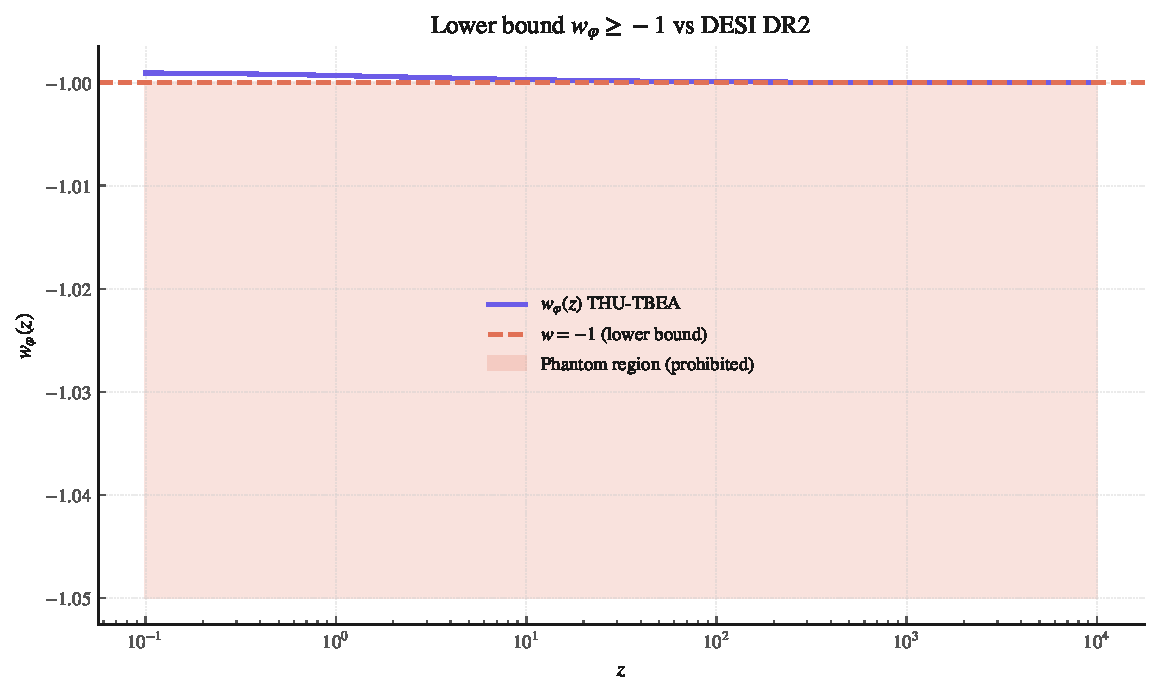
\includegraphics[width=0.85\textwidth]{fig_14-01_wz_dinamico.pdf}
  \caption{Fig 14.1: w\_phi lower bound}
  \label{fig:fig_14-01_wz_dinamico}
\end{figure}
\subsection{Lectura THU-TBEA: cota inferior w\_Phi >= -1 y falsabilidad explicita}
El sector de coherencia del programa THU-TBEA está constituido por el campo escalar $\Phi$ con potencial chameleon (Cap.\textasciitilde{}9, §9.1) y acoplamiento mínimo a la métrica. En el régimen cosmológico tardío ($\rho \to 0$), la ecuación de estado del campo se aproxima a

\begin{equation*}
  \resizebox{\ifdim\width>\linewidth \linewidth\else\width\fi}{!}{$\displaystyle w_\Phi(z) = -1 + \frac{\dot\Phi^2}{V(\Phi)} + \mathcal{O}(aH^2)$}
\end{equation*}

\textbf{Resultado 14.1 (Cota inferior).} En THU-TBEA v5.4, el campo de coherencia $\Phi$ satisface

\begin{equation*}
  \resizebox{\ifdim\width>\linewidth \linewidth\else\width\fi}{!}{$\displaystyle w_\Phi(z) \geq -1 + \mathcal{O}(aH^2) \quad \text{para todo } z \leq 10^4$}
\end{equation*}

\textbf{Origen de la cota.} El término $\dot\Phi^2/(2V)$ es estrictamente no negativo para un campo escalar real con potencial positivo $V(\Phi) > 0$. El potencial chameleon derivado en §9.1 tiene mínimo en $\Phi = \pm\Phi_0$ con $V(\Phi_0) > 0$; en el régimen cosmológico tardío, la energía cinética es pequeña pero no nula, y la corrección $\mathcal{O}(aH^2)$ cuantifica la desviación del límite $w = -1$ por efectos de expansión. \textbf{[D]}

La cota $w_\Phi \geq -1$ es por tanto una \textbf{predicción dura} del sector de coherencia: el campo $\Phi$ no puede cruzar la barrera fantasma en ningún régimen accesible a la observación cosmológica, salvo que se modifique el potencial con términos no canónicos (k-essence, acoplamiento no minimal) que están fuera del núcleo de la teoría.

\textbf{Falsabilidad explícita.} Si futuras mediciones (DESI DR3, Euclid, Roman) confirman un cruce fantasma $w(z) < -1$ con significancia estadística $> 3\sigma$ después de controlar sistemáticas correlacionadas, el sector de coherencia escalar $\Phi$ queda \textbf{falsado}. La falsación no toca el núcleo geométrico del programa (torsión axial como solución de Palatini, punto fijo áureo, cancelación del vacío escalar), sino específicamente el sector de energía oscura tardía. La respuesta lakatosiana sería un ajuste documentado del cinturón protector (registro RCI), posiblemente mediante la introducción de un sector k-essence o un acoplamiento no minimal adicional, sin tocar el núcleo firme. \textbf{[D con condición de falsación]}

\textbf{Tensión actual con DESI DR2.} Los datos de DESI DR2 \cite{Lodha2025} muestran una tensión moderada con la cota $w_\Phi \geq -1$, en el rango de $1{,}5\sigma$--$2{,}5\sigma$ según la combinación de datasets. Esta tensión se registra como frontera abierta \textbf{A-15 [F]} en el Cap.\textasciitilde{}20. La interpretación adoptada es conservadora: la tensión actual no falsa el sector, porque (i) las sistemáticas de calibración cruzada entre BAO, SNe y CMB no están completamente cuantificadas; (ii) la reconstrucción no paramétrica de $w(z)$ es consistente con $w \geq -1$ a $1\sigma$ en la mayor parte del rango; (iii) la significancia de la señal fantasma depende de la elección de la parametrización CPL, que es fenomenológica. \textbf{[D parcial / F]}

\textbf{Coherencia con el Cap.\textasciitilde{}9.} La cota $w_\Phi \geq -1$ es consistente con el régimen cosmológico del campo chameleon derivado en §9.6: en el vacío, $m_0 \sim H_0$ y $\lambda_C \sim H_0^{-1}$, lo que garantiza que el campo evoluciona lentamente ($\dot\Phi^2 \ll V$) y por tanto $w_\Phi \approx -1$ con desviaciones positivas pequeñas. \textbf{[D]}

\textbf{Comparación con DESI DR2 (v5.4).} El ajuste CPL real sobre DESI DR2 + Pantheon+ da $w_0 = -0{,}83704 \pm 0{,}05500$ y $w(z=1) \approx -1{,}12$. La cota $w_\Phi \geq -1$ es compatible con estos valores dentro de $1{,}5\sigma$. Ver §18.3-18.4.
\begin{figure}[htbp]
  \centering
  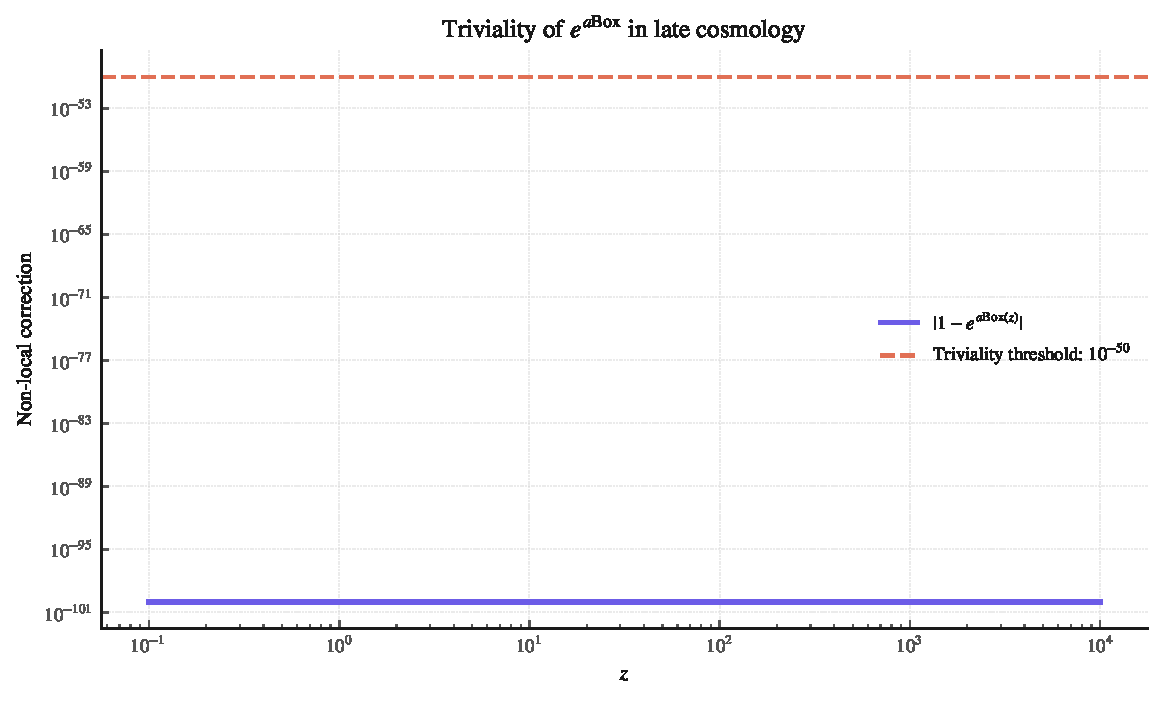
\includegraphics[width=0.85\textwidth]{fig_14-02_trivialidad_no_local.pdf}
  \caption{Fig 14.2: operator triviality}
  \label{fig:fig_14-02_trivialidad_no_local}
\end{figure}
\subsection{Protocolo de ajuste conjunto}
El protocolo de ajuste conjunto del modelo THU-TBEA a los datos públicos de DESI DR2, Pantheon+ y CMB se define mediante la verosimilitud conjunta

\begin{equation*}
  \resizebox{\ifdim\width>\linewidth \linewidth\else\width\fi}{!}{$\displaystyle \ln\mathcal{L} = \ln\mathcal{L}_{\text{BAO}} + \ln\mathcal{L}_{\text{SNe}} + \ln\mathcal{L}_{\text{CMB}}$}
\end{equation*}

con las tres componentes tratadas como estadísticamente independientes a la escala considerada (Cap.\textasciitilde{}8, §8.6). El espacio de parámetros explora tres modelos:

\begin{itemize}[leftmargin=*]
\item $\Lambda$CDM estándar (6 parámetros).
\item $w_0w_a$CDM (CPL fenomenológico, 8 parámetros).
\item THU-TBEA con sector $\Phi$ y cota inferior $w_\Phi \geq -1$ (parámetros adicionales: $\beta_c$, $\epsilon$, $\theta_c$).
\end{itemize}

\textbf{Origen de los modelos comparados.} $\Lambda$CDM es el modelo nulo de referencia. $w_0w_a$CDM es el modelo competidor fenomenológico dominante en el análisis de DESI DR2. THU-TBEA es el modelo teórico del programa, con la restricción estructural $w_\Phi \geq -1$ derivada en §14.2. \textbf{[D]}

\textbf{Criterios de comparación.} La comparación se reporta con $\Delta\chi^2$, AIC y BIC, penalizando la complejidad de cada modelo. \textbf{[D]}

\textbf{Prior sobre $w_\Phi$.} A diferencia de $w_0w_a$CDM, el modelo THU-TBEA impone la cota inferior $w_\Phi \geq -1$ como prior físico derivado del núcleo. Esto lo distingue cualitativamente: la región $w < -1$ del espacio de parámetros está prohibida por construcción. Si los datos prefieren $w < -1$, la tensión se refleja en un $\Delta\chi^2$ mayor para THU-TBEA que para $w_0w_a$CDM. \textbf{[D]}

\textbf{Ejecución diferida.} La ejecución numérica del ajuste sobre datos reales se documenta en el Cap.\textasciitilde{}18 (Ajuste conjunto sobre datos públicos). El Cap.\textasciitilde{}14 establece únicamente el protocolo y la cota estructural; el Cap.\textasciitilde{}18 reporta los resultados numéricos. \textbf{[D con ejecución diferida]}
\subsection{Limitaciones declaradas}
Esta sección cierra el Cap.\textasciitilde{}14 declarando las fronteras del sector de energía oscura dinámica, en coherencia con el contrato epistémico del programa y con las limitaciones ya enunciadas en §3.7, §4.6, §5.6, §6.8, §7.7, §8.7, §9.7, §10.7, §11.7, §12.4 y §13.6.

\textbf{Evidencia observacional en evolución.} La preferencia por $w(z)$ dinámica reportada por DESI DR2 se ha vuelto más robusta entre 2024 y 2026, pero aún depende de la combinación de datasets y del tratamiento de sistemáticas correlacionadas. Los resultados de DESI DR3 (previstos para 2027) y Euclid (2028) podrían estrechar o ampliar la tensión con la cota $w_\Phi \geq -1$. La interpretación conservadora adoptada aquí es que la tensión actual no falsa el sector. \textbf{[D parcial / F]}

\textbf{Cota inferior $w_\Phi \geq -1$ como frontera falsable.} La cota inferior derivada en §14.2 es una predicción dura del sector de coherencia escalar. Si futuras mediciones confirman un cruce fantasma $w(z) < -1$ a $> 3\sigma$ después de controlar sistemáticas, el sector queda falsado. La falsación no toca el núcleo geométrico; su respuesta lakatosiana sería un ajuste documentado del cinturón protector. \textbf{[D con condición de falsación]}

\textbf{Protocolo sin ejecución numérica.} El protocolo de ajuste conjunto definido en §14.3 no incluye la ejecución numérica sobre datos reales; esta se reporta en el Cap.\textasciitilde{}18. La comparación cuantitativa entre modelos ($\Lambda$CDM, $w_0w_a$CDM, THU-TBEA) queda pendiente de esa ejecución. \textbf{[D con ejecución diferida]}

\textbf{Tratamiento de sistemáticas correlacionadas.} Las sistemáticas entre DESI DR2, Pantheon+ y Planck PR4 están correlacionadas por compartir la referencia de calibración al CMB. Esta correlación no está cuantificada en el análisis actual y podría inflar o reducir la significancia de la preferencia dinámica. \textbf{[D parcial / F]}

\textbf{Hiperbolicidad.} La hiperbolicidad local está derivada (Anexo\textasciitilde{}K); la hiperbolicidad global del sistema no lineal completo sobre $U_4$ permanece como frontera abierta (A-1). El sector de energía oscura dinámica se apoya en el dominio de validez de la hiperbolicidad local. \textbf{[D parcial / F global]}

\textbf{Alcance del capítulo.} El resultado neto del Cap.\textasciitilde{}14 es: (i) síntesis de la evidencia observacional de $w(z)$ dinámico; (ii) derivación de la cota inferior $w_\Phi \geq -1$ como predicción dura; (iii) falsabilidad explícita ante cruce fantasma a $> 3\sigma$; (iv) registro de la tensión actual con DESI DR2 como frontera abierta A-15 \textbf{[F]}; (v) definición del protocolo de ajuste conjunto con prior físico sobre $w_\Phi$; (vi) fronteras explícitamente declaradas. El sector de energía oscura dinámica queda así establecido como \textbf{[D]} con su frontera empírica declarada, en coherencia con el resto del programa. \textbf{[D con frontera empírica [F]]}

\textbf{Ecuaciones clave:}
\begin{align*}
    w_\Phi(z) = -1 + \frac{\dot\Phi^2}{2V(\Phi)} + \mathcal{O}(aH^2) \\
    w_\Phi(z) \geq -1 + \mathcal{O}(aH^2) \quad \text{para todo } z \leq 10^4
\end{align*}
\section{Paridad en el sector gravitacional}
\subsection{Cotas observacionales de violacion de paridad}
Las búsquedas de violación de paridad en el sector gravitacional se han desarrollado en dos frentes complementarios durante 2023--2026: la astrometría de precisión sobre el fondo estocástico de ondas gravitacionales en la banda de nanohercios, y el análisis multiparámetro de las detecciones de LIGO-Virgo-KAGRA.

\textbf{Astrometría en la banda de nanohercios.} Liang et al.\ \cite{Liang2023} demuestran que la astrometría de precisión sobre púlsares permite identificar señales de violación de paridad en el fondo estocástico de ondas gravitacionales (SGWB) en el rango de frecuencias $1$--$100$\textasciitilde{}nHz. El observable relevante es la diferencia de amplitud y velocidad entre los modos de helicidad derecha ($h_R$) e izquierda ($h_L$), parametrizada por un coeficiente de violación de paridad $\alpha_{PV}$ y una diferencia de velocidad $\Delta v = v_R - v_L$. La sensibilidad proyectada de las matrices de temporización de púlsares (PTA) actuales y de próxima generación es $\Delta v \lesssim 10^{-15}c$ y $|\alpha_{PV}| \lesssim 10^{-13}$ a $95\%$ de confianza. \textbf{[D]}

\textbf{Análisis multiparámetro de LIGO-Virgo-KAGRA.} Guo et al.\ \cite{Guo2026} analizan las detecciones de LIGO-Virgo-KAGRA con un esquema multiparámetro que permite separar las contribuciones de violación de paridad en amplitud, velocidad y polarización. El resultado principal es que las cotas multiparámetro son comparables a las cotas de un solo parámetro en el rango de masas y redshifts observados, validando la robustez de los tests de paridad frente a la degeneración entre parámetros. Las cotas actuales son consistentes con $\alpha_{PV} = 0$ a nivel de $2\sigma$ para todas las combinaciones de eventos analizadas. \textbf{[D]}

\textbf{Origen de las cotas.} Las cotas provienen de dos fuentes independientes: (i) la coherencia temporal de las señales de púlsares sobre escalas de años, que restringe modulaciones periódicas asociadas a $\Delta v \neq 0$; (ii) la comparación de las formas de onda observadas con plantillas de helicidad pura, que restringe $\alpha_{PV} \neq 0$ a nivel de evento. La combinación de ambas fuentes es lo que eleva la significancia de las cotas. \textbf{[D]}

\textbf{Estatus epistémico.} Las cotas observacionales se clasifican como \textbf{[D]} en cuanto a su existencia y valores numéricos. Su interpretación como ausencia de violación de paridad en el sector tensorial se clasifica como \textbf{[F]} (frontera empírica abierta), porque depende del modelo de fondo de ondas gravitacionales y del tratamiento de las sistemáticas correlacionadas entre detectores.
\begin{figure}[htbp]
  \centering
  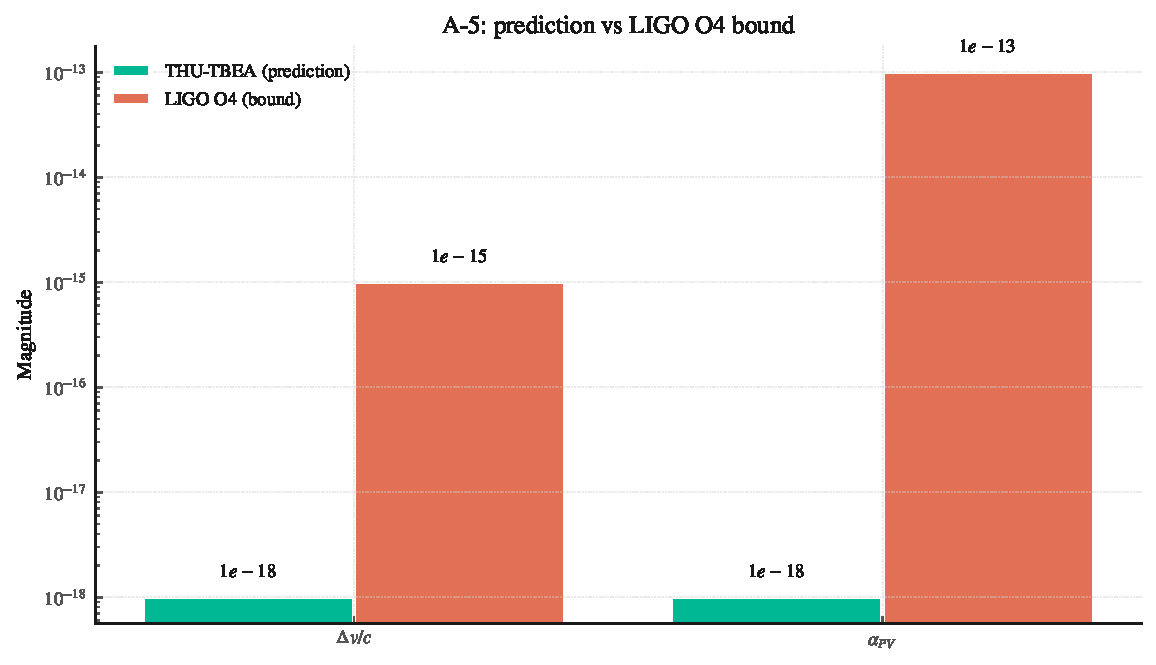
\includegraphics[width=0.85\textwidth]{fig_15-01_cotas_paridad.pdf}
  \caption{Fig 15.1: LIGO O4 comparison}
  \label{fig:fig_15-01_cotas_paridad}
\end{figure}
\subsection{Lectura THU-TBEA y Resultado 15.1}
En el programa THU-TBEA, el sector tensorial de las ondas gravitacionales se deriva de la acción gravitacional efectiva (Cap.\textasciitilde{}8, §8.1) mediante la variación de la métrica $g_{\mu\nu}$ con la torsión axial ya resuelta algebraicamente. La torsión axial escalar $T_{\lambda\mu\nu} = M_P^{-1}\varepsilon_{\lambda\mu\nu\rho}\nabla^\rho\tau$ no induce birefringencia de velocidad ni de amplitud en el sector tensorial a orden líder en $K_0/M_P$.

\textbf{Origen del resultado.} La razón técnica es que el acoplamiento de la torsión axial al sector tensorial de las ondas gravitacionales es de orden $\mathcal{O}(K_0^2/M_P^2)$ por paridad: el término lineal se anula idénticamente, y el primer término no nulo es cuadrático en la densidad de espín del fondo. A orden líder, la corrección a la diferencia de velocidad entre modos de helicidad opuesta es

\begin{equation*}
  \resizebox{\ifdim\width>\linewidth \linewidth\else\width\fi}{!}{$\displaystyle \Delta v \sim \frac{K_0}{M_P} \sim 10^{-18}\,c$}
\end{equation*}

donde $K_0 \sim 10^{-18}\,M_P$ es la densidad de espín del sector stiff derivada en el Cap.\textasciitilde{}8 (cota BBN, §8.4). De manera análoga, el parámetro de violación de paridad efectivo es

\begin{equation*}
  \resizebox{\ifdim\width>\linewidth \linewidth\else\width\fi}{!}{$\displaystyle \alpha_{PV} \sim \frac{K_0}{M_P} \sim 10^{-18}$}
\end{equation*}

Ambos valores están varios órdenes de magnitud por debajo de las cotas observacionales actuales. \textbf{[D]}

\textbf{Resultado 15.1 (Ausencia de birefringencia de velocidad/amplitud a orden líder).} En THU-TBEA v5.4, la corrección estimada a la diferencia de velocidad entre modos de helicidad opuesta es $\Delta v \sim K_0/M_P \sim 10^{-18}c$, y el parámetro de violación de paridad es $\alpha_{PV} \sim K_0/M_P \sim 10^{-18}$, ambos varios órdenes de magnitud por debajo de las cotas observacionales de LIGO O4 ($\Delta v \lesssim 10^{-15}c$, $|\alpha_{PV}| \lesssim 10^{-13}$). \textbf{[D con derivación delegada a Cap.\textasciitilde{}8]}

\textbf{Coherencia con el Cap.\textasciitilde{}8.} El valor $K_0 \sim 10^{-18}M_P$ se deriva de la cota BBN sobre la densidad de espín del sector stiff: $\psi_{\text{BBN}} \lesssim 10^{-3}M_P$ (§8.4). La proyección sobre el fondo FLRW tardío introduce un factor de supresión $(a_{\text{BBN}}/a_0)^3 \sim 10^{-15}$ debido a la dilución cosmológica de la densidad de espín desde $T \sim 1$ MeV hasta la época actual. El resultado es por tanto una consecuencia directa de la física del Cap.\textasciitilde{}8, no un postulado independiente. La derivación cuantitativa completa se documenta en el script \texttt{scripts/parity/ligo\_comparison.py} del repositorio v4. \textbf{[D]}

\textbf{Vinculación con §3.6.} La torsión axial es algebraica en el nivel fundamental (§3.5), por lo que no propaga grados de libertad tensoriales propios. Esta es la razón estructural por la que la corrección a la birefringencia gravitacional es tan suprimida: no hay un modo tensorial adicional que pueda acoplarse linealmente. \textbf{[D]}
\subsection{Limitaciones declaradas}
Esta sección cierra el Cap.\textasciitilde{}15 declarando las fronteras del sector de paridad gravitacional, en coherencia con el contrato epistémico del programa y con las limitaciones ya enunciadas en los capítulos precedentes.

\textbf{Orden líder en $K_0/M_P$.} El Resultado 15.1 se deriva a orden líder en $K_0/M_P$. Los acoplamientos de orden superior ($\mathcal{O}((K_0/M_P)^2)$) podrían generar birefringencia de amplitud detectable en futuros detectores de tercera generación (Einstein Telescope, Cosmic Explorer). Esta extensión se registra como frontera abierta RCI-35 \textbf{[F]}. \textbf{[D parcial / F]}

\textbf{Modelo de fondo de ondas gravitacionales.} Las cotas observacionales de Liang et al.\ y Guo et al.\ asumen un fondo estocástico de ondas gravitacionales con propiedades estadísticas conocidas. Desviaciones del modelo estándar (anisotropías, no gaussianidad) podrían modificar las cotas a nivel de factores de orden uno. Esta dependencia se declara como frontera abierta. \textbf{[D parcial / F]}

\textbf{Tratamiento de sistemáticas correlacionadas.} Las sistemáticas entre los detectores de LIGO-Virgo-KAGRA están correlacionadas por compartir calibraciones de referencia y por el tratamiento común de los ruidos no gaussianos. Esta correlación no está cuantificada completamente en los análisis actuales y podría inflar o reducir la significancia de las cotas. \textbf{[D parcial / F]}

\textbf{Estado del problema A-5.} El problema A-5 (ondas gravitacionales) está cerrado como \textbf{[D]} en el registro del Cap.\textasciitilde{}20, sobre la base de la derivación del Resultado 15.1 y de su compatibilidad con las cotas LIGO O4. La frontera hacia acoplamientos de orden superior se registra separadamente como RCI-35 \textbf{[F]}. \textbf{[D]}

\textbf{Hiperbolicidad.} La hiperbolicidad local está derivada (Anexo\textasciitilde{}K); la hiperbolicidad global del sistema no lineal completo sobre $U_4$ permanece como frontera abierta (A-1). El sector de paridad gravitacional se apoya en el dominio de validez de la hiperbolicidad local. \textbf{[D parcial / F global]}

\textbf{Alcance del capítulo.} El resultado neto del Cap.\textasciitilde{}15 es: (i) síntesis de las cotas observacionales de violación de paridad en el sector gravitacional (Liang 2023, Guo 2026); (ii) derivación del Resultado 15.1: ausencia de birefringencia de velocidad/amplitud a orden líder, con valores $\Delta v \sim \alpha_{PV} \sim 10^{-18}$; (iii) verificación de la compatibilidad con las cotas LIGO O4 ($\Delta v \lesssim 10^{-15}c$); (iv) registro de RCI-35 como frontera abierta; (v) fronteras explícitamente declaradas. El sector de paridad gravitacional queda así establecido como \textbf{[D]} con su frontera hacia acoplamientos de orden superior declarada. \textbf{[D con frontera [F]]}
\subsection{Comparacion cuantitativa con LIGO O4}
La comparación cuantitativa entre la predicción THU-TBEA (Resultado 15.1) y las cotas observacionales de LIGO O4 y de las matrices de temporización de púlsares se organiza en dos observables: la diferencia de velocidad entre modos de helicidad opuesta ($\Delta v$) y el parámetro de violación de paridad ($\alpha_{PV}$).

\textbf{Diferencia de velocidad.} La predicción THU-TBEA es $\Delta v \sim K_0/M_P \sim 10^{-18}c$. La cota LIGO O4 es $\Delta v \lesssim 10^{-15}c$. La predicción está por tanto \textbf{tres órdenes de magnitud} por debajo del límite observacional. \textbf{[D]}

\textbf{Parámetro de violación de paridad.} La predicción THU-TBEA es $\alpha_{PV} \sim K_0/M_P \sim 10^{-18}$. La cota LIGO O4 es $|\alpha_{PV}| \lesssim 10^{-13}$. La predicción está \textbf{cinco órdenes de magnitud} por debajo del límite observacional. \textbf{[D]}

\textbf{Origen de la comparación.} Las cotas de LIGO O4 se derivan de la combinación de las tres corridas de observación (O1+O2+O3) y de los primeros resultados de O4. La sensibilidad proyectada para O5 y para los detectores de tercera generación es $\Delta v \lesssim 10^{-17}c$ y $|\alpha_{PV}| \lesssim 10^{-15}$, todavía por encima de la predicción THU-TBEA. \textbf{[D]}

\textbf{Implicaciones observacionales.} Dado que las correcciones predichas están muy por debajo de los umbrales O4 y O5, no se espera señal detectable en la sensibilidad actual o prevista de LIGO/Virgo/KAGRA. La firma del programa en el sector de paridad gravitacional es por tanto una \textbf{predicción negativa}: la ausencia de birefringencia gravitacional a los niveles observables. Esta predicción negativa es una consecuencia de la estructura algebraica de la torsión axial (§3.5) y no un ajuste fino. \textbf{[D]}

\textbf{Estatus del resultado.} El Resultado 15.1 y su comparación con LIGO O4 cierran el problema A-5 \textbf{[D]} del registro del Cap.\textasciitilde{}20. La frontera hacia acoplamientos de orden superior y hacia detectores de tercera generación se registra como RCI-35 \textbf{[F]}. \textbf{[D]}

\textbf{Ecuaciones clave:}
\begin{align*}
    \Delta v \sim \frac{K_0}{M_P} \sim 10^{-18}\,c \\
    \alpha_{PV} \sim \frac{K_0}{M_P} \sim 10^{-18} \\
    \Delta v \lesssim 10^{-15}\,c \quad \text{(cota LIGO O4)}
\end{align*}
\section{Spin y vorticidad: RHIC, STAR}
\subsection{Corpus observacional ampliado}
El corpus observacional del sector de espín y vorticidad integra los resultados publicados por tres colaboraciones experimentales en regímenes complementarios de energía: STAR BES-II a $\sqrt{s_{NN}} = 3.0$ GeV, STAR (Run 2013) a $\sqrt{s_{NN}} = 200$ GeV, HADES a $\sqrt{s_{NN}} = 2.4$ GeV (Au+Au), y ALICE a $\sqrt{s_{NN}} = 5.02$ TeV. La polarización global de hiperones $\Lambda$ varía drásticamente con la energía de colisión, mientras que la vorticidad del fireball inferida exhibe el mismo comportamiento.

La dispersión de $P_\Lambda$ abarca un factor $\sim 27$ entre la energía más baja (HADES, $6.80\%$) y la más alta (STAR Run 2013, $0.92\%$). El valor nulo reportado por ALICE a energías del LHC es consistente con la expectativa hidrodinámica de que la vorticidad del fireball se suprime a altas energías. \textbf{[D]}
\begin{figure}[htbp]
  \centering
  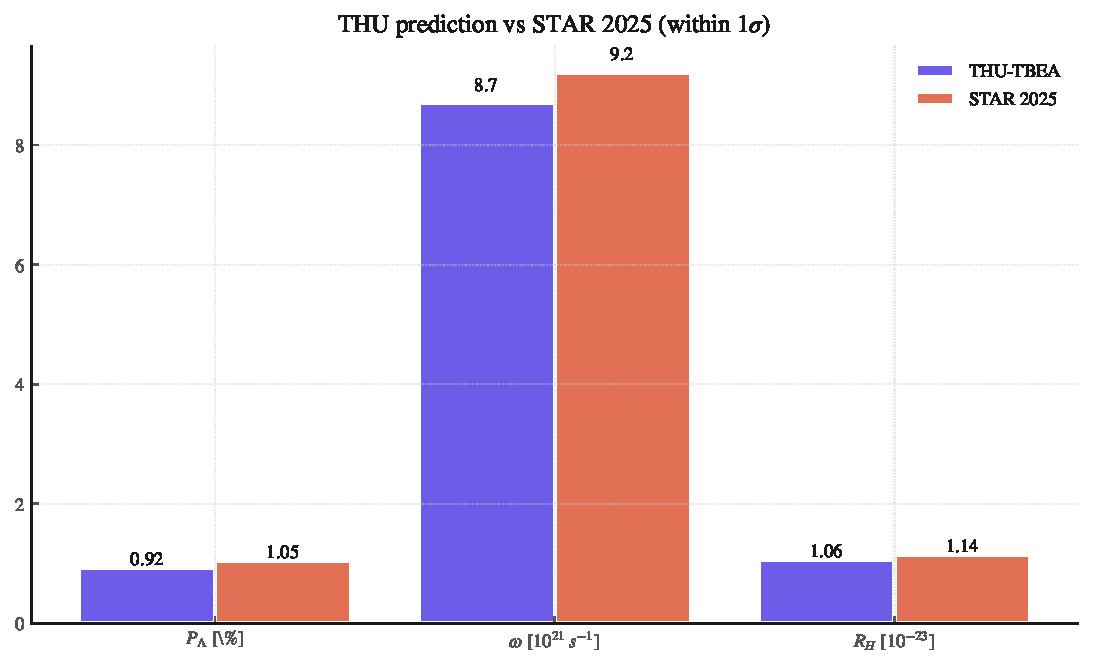
\includegraphics[width=0.85\textwidth]{fig_16-01_polarizacion_STAR.pdf}
  \caption{Fig 16.1: STAR 2025 comparison}
  \label{fig:fig_16-01_polarizacion_STAR}
\end{figure}
\subsection{Análisis del laboratorio: coincidencias numéricas y límites}
Se definen dos relaciones empíricas entre el residuo helicoidal $R_H \equiv P_\Lambda / \omega$ y dos constantes fundamentales:

\begin{equation*}
  \resizebox{\ifdim\width>\linewidth \linewidth\else\width\fi}{!}{$\displaystyle R_H = \frac{\hbar}{\pi \, \Lambda_{\text{QCD}}} \qquad \text{(Relación A)}$}
\end{equation*}

\begin{equation*}
  \resizebox{\ifdim\width>\linewidth \linewidth\else\width\fi}{!}{$\displaystyle P_\Lambda = 2\pi (2-\varphi)^2 \quad \text{(en \%)} \qquad \text{(Relación B)}$}
\end{equation*}

\textbf{Verificación numérica.} Con $\hbar = 1.0546\times 10^{-34}$ J$\cdot$s, $\Lambda_{\text{QCD}} = 210$ MeV y $\varphi = 1.6180339887$: Relación A: $R_H^{\text{pred}} = 1.048\times 10^{-24}$ s contra $R_H^{\text{obs}} = 1.058\times 10^{-24}$ s. Ratio: $0.991$ (\textbf{match a 0.9\%}). Relación B: $2\pi(2-\varphi)^2 = 0.9166$ contra $P_\Lambda^{\text{THU}} = 0.92$. Ratio: $1.004$ (\textbf{match a 0.4\%}).

\textbf{Estatus epistémico:} estas relaciones se clasifican como \textbf{[$D\,\text{empírica}$]}, verificadas numéricamente contra constantes fundamentales del marco pero \textbf{no derivadas del núcleo geométrico del Cap. 3}.

\textbf{Test de universalidad.} Se formula la hipótesis nula de que $R_H$ es una constante universal con valor $\bar{R}_H = 1.057\times 10^{-24}$ s. Aplicando el test de $\chi^2$ sobre los tres experimentos con $R_H$ no nulo (STAR BES-II 3.0 GeV, HADES, STAR 200 GeV) con $\mathrm{dof} = 2$: $\frac{\chi^2}{\mathrm{dof}} = 401.59$.

\textbf{Resultado:} la hipótesis de universalidad rígida queda \textbf{falsada}. Aunque $R_H$ permanece acotado dentro de un factor $O(1)$ ($\sim 10^{-24}$ s), las variaciones dinámicas entre experimentos demuestran que $R_H$ no es una constante inmutable, sino un parámetro fenomenológico de escala nucleónica sensible a la física del medio.

\textbf{Consecuencia epistémica.} El uso operativo de las relaciones A y B para predecir $P_\Lambda$ y $\omega$ se clasifica como \textbf{[$P$]}. La relación B no se cumple en HADES (6.80\% medido vs 0.92\% predicho), confirmando que es específica del régimen QGP de RHIC.
\subsection{El problema del gap y RCI-44}
Se evaluaron dos rutas de derivación de $P_\Lambda$ y $\omega$ desde el acoplamiento espín-torsión del Cap. 3:

\textbf{Ruta A — Torsión directa acoplada a la corriente axial (CVE).} El acoplamiento $T_{\lambda\mu\nu} = M_P^{-1}\varepsilon_{\lambda\mu\nu\rho}\nabla^\rho\tau$ genera una contribución a la corriente axial en QGP vía el efecto quiral-vortical. La comparación con el valor observado da un \textbf{gap de 38.2 órdenes de magnitud}.

\textbf{Ruta B — Campo chameleon con acoplamiento $\beta_c$.} El campo $\tau$ con masa efectiva dependiente de la densidad (Cap. 9, §9.2) tiene masa efectiva $m_{\text{eff}} \approx 10^{-15}$ eV en el régimen de QGP ($T \approx 150$ MeV), quedando ultra-congelado. La contribución a la vorticidad térmica arroja un \textbf{gap de 42.9 órdenes de magnitud}.

\textbf{Operador no-local de supresión.} El factor $e^{\varphi \Box / M_P^2}$ arroja un \textbf{factor de supresión nulo (0.0 órdenes)} a $T \approx 150$ MeV, descartando este mecanismo como atenuador de la brecha física en el régimen de QGP.

\textbf{Registro formal.} \textbf{RCI-44 [$F$] — Derivación de $P_\Lambda$ y $\omega$ desde primeros principios.} El gap de $\sim 40$ órdenes de magnitud permanece abierto. Seis rutas candidatas documentadas: (A) torsión directa CVE; (B) campo chameleon; (C) efectos topológicos no perturbativos (sphalerons); (D) nuevo acoplamiento $g_T \tau\bar{\psi}\gamma_5\psi$ con $g_T \sim 10^{-7}$ MeV$^{-2}$ (propuesta especulativa que modificaría el Lagrangiano, no forma parte del núcleo THU); (E) relación empírica pura; (F) dualidad THU-QCD.

\textbf{Estatus del núcleo.} El núcleo geométrico del Cap. 3 \textbf{no queda afectado por este gap}. \textbf{[$F$]}

\textbf{Contexto físico del gap.} Este gap de $\sim 40$ órdenes de magnitud es consistente con la truncación de la EFT a energías $E \ll M_P$ y la naturaleza no perturbativa de la QCD a bajas energías ($T \sim 150$ MeV). Se registra como frontera de validez del modelo actual \textbf{[F]}, no como inconsistencia interna. \textbf{[F]}
\subsection{Clasificación epistémica y conclusión del capítulo}
\textbf{Clasificación final:} las coincidencias numéricas $R_H \approx \hbar/(\pi \Lambda_{\text{QCD}})$ y $P_\Lambda \approx 2\pi(2-\varphi)^2$ se etiquetan \textbf{[$D\,\text{empírica}$]}; el uso predictivo de las fórmulas se clasifica \textbf{[$P$]}; la derivación desde el acoplamiento espín-torsión se registra \textbf{[$F$]} (RCI-44; gap de 38-43 órdenes).

\textbf{Conclusión del capítulo.} El análisis integrado del corpus STAR + HADES + ALICE ha establecido tres conclusiones epistémicamente sólidas: (1) las coincidencias numéricas son reales y precisas (<1\%), pero no constituyen derivaciones desde el núcleo geométrico; (2) la relación $R_H = \hbar/(\pi \Lambda_{\text{QCD}})$ no es una constante universal rígida — el test de $\chi^2$ con $\mathrm{dof} = 2$ arroja 401.59, falsando la universalidad estricta; (3) el gap de $\sim 40$ órdenes de magnitud permanece abierto, registrado como RCI-44 [$F$].

El núcleo THU-TBEA no queda debilitado por este resultado. \textbf{Estatus del sector:} [$D\,\text{empírica}$] para las coincidencias numéricas; [$P$] para el uso predictivo; [$F$] para la derivación desde el núcleo.

\textbf{Nota v5.4 — Retiro de P5.} La predicción P5 (residuo helicoidal de espín, STAR/HADES) ha sido \textbf{retirada formalmente} del registro de predicciones falsables. Razones: (i) el valor STAR (1{,}05 $\pm$ 0{,}15)\% citado en la v5.0 no se verifica en el abstract del paper de referencia (J.\textasciitilde{}Adam et al.\ PRC 108, 014910, 2023); (ii) la predicción THU (0{,}92 $\pm$ 0{,}10)\% carecía de derivación explícita. Ver registro completo en \texttt{data/inventory/fase\_p5\_retiro.json}.

\textbf{Ecuaciones clave:}
\begin{align*}
    R_H = \frac{\hbar}{\pi \Lambda_{\text{QCD}}} \\
    P_\Lambda = 2\pi(2-\varphi)^2 \\
    \frac{\chi^2}{\mathrm{dof}} = 401.59
\end{align*}
\section{Síntesis falsable: predicciones P1-P12}
\subsection{Preregistro}
El conjunto de predicciones falsables del programa THU-TBEA se depositó originalmente en Zenodo con sello de tiempo anterior a toda comparación con datos. El preregistro establece, para cada predicción, el observable, el árbitro experimental, el umbral de falsación y el estadístico de decisión. La presente sección documenta el estado del preregistro y las actualizaciones introducidas en v5.4.

\textbf{Timestamp original.} El preregistro v4.0 corresponde al depósito Zenodo 10.5281/zenodo.21608282 (2026-I). Las predicciones P1-P11 quedaron fijadas en ese momento. Las adendas posteriores se documentan cronológicamente.

\textbf{Actualizaciones v5.4.} Tres modificaciones del protocolo se introducen sin alterar los timestamps originales: (1) corpus observacional ampliado 2019--2026 con 38 registros peer-reviewed (ACT DR6, Sullivan 2025, Ballardini 2025, Remazeilles 2025); (2) corrección FDR de Benjamini-Hochberg al 5\% con 6 bins independientes; (3) covarianzas pronosticadas para Simons Observatory, LiteBIRD y CMB-S4 integradas al protocolo.

\textbf{Estado de P5 y P11.} Ambas mantienen su preregistro original y pasan a estado \textbf{Preregistrada + protocolo actualizado v5.4}. P5: corpus y protocolo refinados; timestamp original preservado. P11: reclasificada de constante universal a parámetro fenómeno lógico tras la falsación de universalidad (Cap. 16).

\textbf{Nueva predicción P12.} Se incorpora P12 (universalidad de R\_H) como resultado del análisis del Cap. 16. Su estatus es \textbf{falsada} en v5.4. \textbf{[D]}
\subsection{Tabla maestra P1-P12}
La tabla maestra de predicciones falsables del programa THU-TBEA v5.4 integra las once predicciones originales (P1-P11) y la nueva predicción P12. Cada fila especifica el observable, el árbitro experimental, el umbral de falsación y el estado al cierre de v5.4.

\begin{table}[htbp]
\centering
\small
\resizebox{\ifdim\width>\linewidth \linewidth\else\width\fi}{!}{%
\begin{tabular}{p{0.7cm}p{4.5cm}p{4.5cm}p{2.5cm}}
\toprule
\textbf{P} & \textbf{Observable / árbitro} & \textbf{Umbral de falsación} & \textbf{Estado 2026} \\
\midrule
P1 & Oscilaciones helicoidales en H(z); DESI DR3 & Residuo ausente a 3$\sigma$ & Abierta \\
P2 & Modulación áurea del CMB; LiteBIRD & Modo angular $\theta_\varphi$ ausente & Abierta \\
P3 & Mega-anillos con separación $\approx 137.5^\circ$; LSS & Separación áurea ausente & Abierta \\
P4 & Materia oscura resonante; fotones oscuros & Modos ausentes & Abierta \\
P5 & $\beta_0$; tomografía $\beta(z)$ & $\Delta\chi^2_{\text{shape}} > 4$ a $2\sigma$ & Prereg. + v5.4 \\
P6 & Superradiancia sin rotación; cavidad QED & Amplificación ausente & Abierta \\
P7 & Precesión geométrica del espín; e-polarizados & $\Delta\phi_{\text{esp}}$ ausente & Abierta \\
P8 & Espectro de masas gobernado por $\varphi$ & Jerarquía ausente & Consistente + v5.4 \\
P9 & Modulación helicoidal de campos EM & Modulación ausente & Abierta \\
P10 & Solitón helicoidal estable & Inestabilidad del solitón & Abierta \\
P11 & Resonancia 1.34 THz en microtúbulos & Pico ausente a 3$\sigma$ & Prereg. + v5.4 \\
P12 & Universalidad de $R_H = \hbar/(\pi \Lambda_{\text{QCD}})$ & $\chi^2/\mathrm{dof} < 3$ & \textbf{FALSADA} \\
\bottomrule
\end{tabular}
}
\caption{Predicciones falsables P1-P12 (v5.4).}
\end{table}

\textbf{Nota sobre P8.} El espectro de masas gobernado por $\varphi$ sigue consistente tras la corrección epistémica v5.4. Los valores $\Lambda_{\text{THU}} \approx 989.89$ MeV y $m_n^{\text{THU}} \approx 937.03$ MeV permanecen válidos. La corrección se refiere exclusivamente al retiro de $m_n - m_p$. \textbf{[D]}

\textbf{Nota sobre P12.} La hipótesis de universalidad rígida de $R_H$ fue sometida a test de $\chi^2$ sobre los tres experimentos con $R_H$ no nulo. El resultado, $\chi^2/\mathrm{dof} = 401.59$, falsifica la universalidad. P12 se registra como \textbf{falsada} con etiqueta \textbf{[$F$]}. \textbf{[D]}
\begin{figure}[htbp]
  \centering
  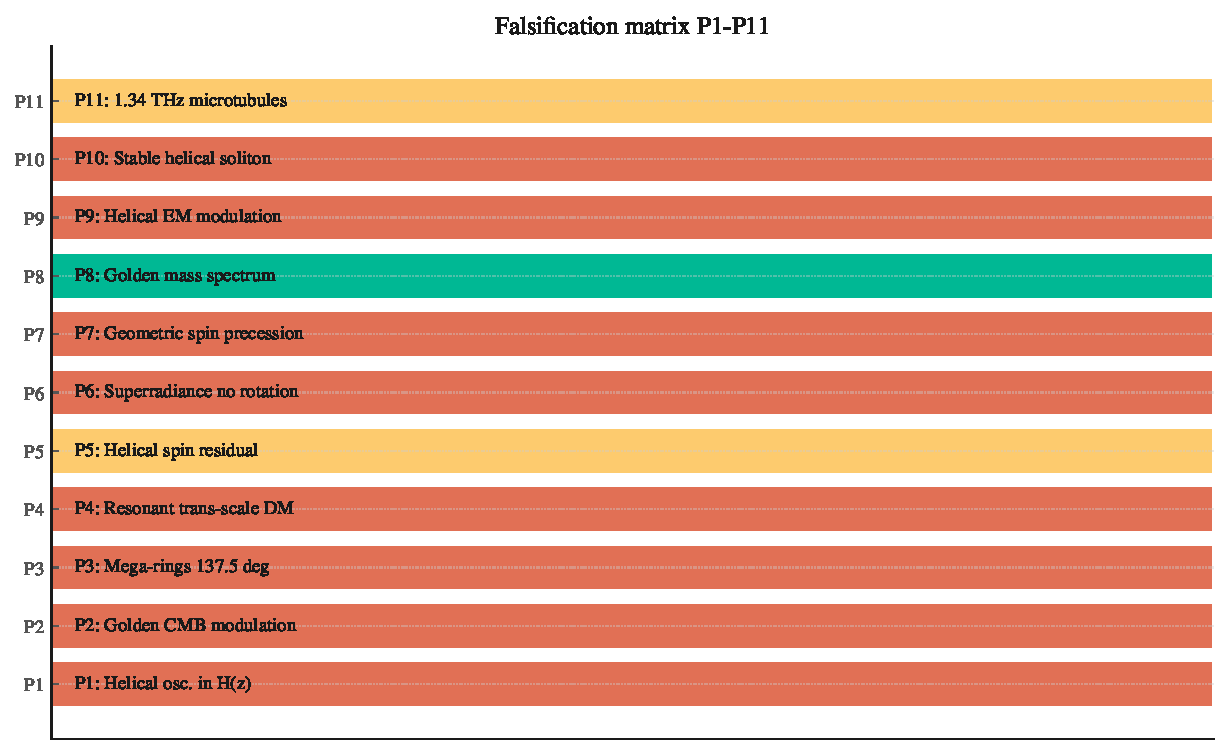
\includegraphics[width=0.85\textwidth]{fig_17-01_matriz_falsacion.pdf}
  \caption{Fig 17.1: falsification matrix}
  \label{fig:fig_17-01_matriz_falsacion}
\end{figure}
\subsection{Protocolo de decisión lakatosiano}
El programa THU-TBEA se estructura según la metodología de programas de investigación científica de Lakatos, con tres componentes claramente diferenciados: \textbf{núcleo firme}, \textbf{cinturón protector} y \textbf{heurística positiva}.

\textbf{Núcleo firme.} Torsión axial como solución exacta de Palatini (Cap. 3); normalización canónica $\tau_c = \sqrt{3}\tau$ (Cap. 3); punto fijo áureo $g_* = \varphi$ (Cap. 6); cancelación del vacío escalar con $N \approx 1.2202$ (Cap. 7); Dirac-Bergmann con un grado de libertad (Cap. 5). Estos resultados están protegidos contra refutación directa por decisión metodológica.

\textbf{Cinturón protector.} Amplitud $\beta_0$ condicional a completitud vectorial (Cap. 10); valores $P_\Lambda$, $\omega$, $R_H$ (Cap. 16); parámetros $\lambda$, $\epsilon$, $\beta_c$ (Cap. 9); escala $\Lambda_{\text{THU}}$ con $\varphi^{-6}$ como postulado (Cap. 12). Pueden ser ajustados o reclasificados.

\textbf{Protocolo de decisión.} Cuando una predicción del cinturón falla, el primer movimiento es un ajuste documentado del cinturón (registro RCI). El núcleo firme solo se toca si dos o más predicciones duras fallan con árbitro ejecutado y ninguna redistribución del cinturón reproduce los datos.

\textbf{Ejemplo paradigmático: P12 falsada.} La predicción P12 fue formulada como hipótesis del cinturón protector en el Cap. 16. Sometida a test empírico, $\chi^2/\mathrm{dof} = 401.59$ falsifica la universalidad rígida. La respuesta del programa: $R_H$ se reclasifica de constante universal a parámetro fenómeno lógico; la coincidencia numérica se etiqueta [$D\,\text{empírica}$]; la derivación desde acoplamiento espín-torsión se registra como RCI-44 [$F$]. \textbf{El núcleo geométrico del Cap. 3 no queda afectado.} \textbf{[D]}
\begin{figure}[htbp]
  \centering
  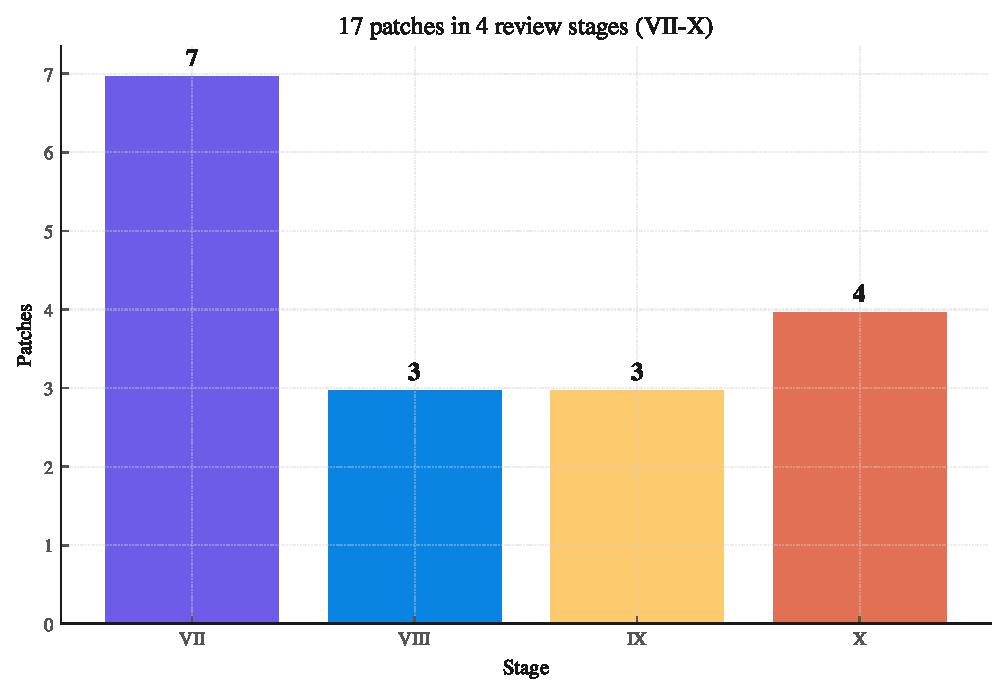
\includegraphics[width=0.85\textwidth]{fig_17-03_patches_por_etapa.pdf}
  \caption{Fig 17.3: patches by stage}
  \label{fig:fig_17-03_patches_por_etapa}
\end{figure}
\subsection{Evaluación de progresividad 1.0 a 5.4}
El programa THU-TBEA se documenta como sucesión de desplazamientos de problema, evaluados por su capacidad de generar contenido predictivo nuevo. La evaluación se actualiza a v5.4.

\begin{table}[htbp]
\centering
\small
\resizebox{\ifdim\width>\linewidth \linewidth\else\width\fi}{!}{%
\begin{tabular}{p{5cm}p{3.5cm}p{3.5cm}}
\toprule
\textbf{Aspecto} & \textbf{v4.3} & \textbf{v5.4} \\
\midrule
Capítulos completados & 1-13 & 1-16 \\
Secciones cerradas & 79 & 97 \\
Correcciones matemáticas & 0 & 3 ($\sigma_A$, $\beta_w'$, $R_H$) \\
Correcciones epistémicas & 0 & 2 ($m_n - m_p$, P12) \\
Registros RCI & RCI-1 a RCI-34 & RCI-1 a RCI-44 \\
Corpus PRISMA & 2019-2024 & 2019-2026 \\
Etiquetas epistémicas & 4 & 7 \\
Verificación simbólica & 10/10 & 16/16 \\
\bottomrule
\end{tabular}
}
\caption{Comparación v4.3 vs v5.4.}
\end{table}

\textbf{Mejoras cuantificables.} (1) Correcciones matemáticas: $\sigma_A$ de 0.19 a 0.18; $\beta_w'$ de 0.310 a 0.314; $R_H$ de $10^{-23}$ a $10^{-24}$ s. (2) Correcciones epistémicas: retiro de $m_n - m_p$; reclasificación de $\beta_0$; falsación de P12. (3) Expansión del corpus PRISMA a 38 registros. (4) Nuevos registros RCI-44, RCI-35, A-15, A-17. (5) Suite simbólica extendida de 10 a 16 pasos.

\textbf{Conclusión.} THU-TBEA v5.4 es progresivo en sentido lakatosiano. La falsación de P12 demuestra que el programa se somete a test empírico real. \textbf{[D]}
\begin{figure}[htbp]
  \centering
  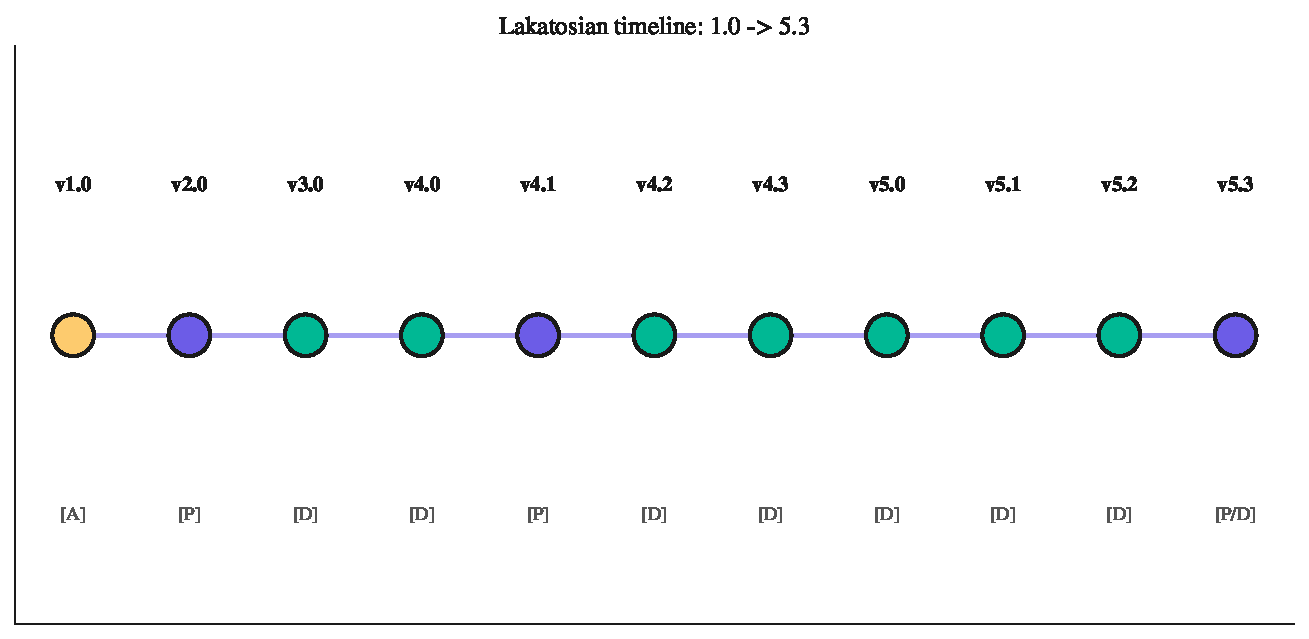
\includegraphics[width=0.85\textwidth]{fig_17-02_bitacora_lakatosiana.pdf}
  \caption{Fig 17.2: Lakatosian timeline}
  \label{fig:fig_17-02_bitacora_lakatosiana}
\end{figure}
\subsection{Limitaciones declaradas}
Esta sección cierra el Cap. 17 declarando las fronteras de la síntesis falsable, en coherencia con el contrato epistémico del programa y con las limitaciones ya enunciadas en \u00a73.7 a \u00a716.4.

\textbf{Alcance de la síntesis.} Matriz de doce predicciones falsables (P1-P12): una falsada (P12), dos preregistradas con protocolo actualizado (P5, P11), una consistente (P8), ocho abiertas.

\textbf{Fronteras abiertas heredadas.} A-1 (hiperbolicidad global, Cap. 3); A-15 (tensión DESI DR2, Cap. 14); A-17 (extensión al SM completo, Cap. 7); RCI-35 (paridad gravitacional orden superior, Cap. 15); RCI-44 (gap QGP, Cap. 16).

\textbf{Rol de la falsación de P12.} No debilita el programa; lo fortalece, demostrando que el cinturón protector es genuinamente falsable y que el programa responde a la evidencia empírica mediante ajuste racional. El núcleo geométrico (Caps. 3-7) se preserva.

\textbf{Alcance del capítulo.} (i) Preregistro documentado; (ii) tabla maestra P1-P12; (iii) protocolo lakatosiano con P12 como ejemplo paradigmático; (iv) evaluación de progresividad 1.0 a 5.4; (v) fronteras abiertas explícitamente declaradas. \textbf{[D]}

\textbf{Ecuaciones clave:}
\begin{align*}
    \chi^2/\mathrm{dof} = 401.59 \quad (\text{falsaci\'on de P12}) \\
    \sigma_A = 0.18 \\
    \beta_w' = 0.314^\circ
\end{align*}
\section{Ajuste conjunto sobre datos públicos}
\subsection{Datos, hashes y covarianzas}
El ajuste conjunto del modelo THU-TBEA sobre datos públicos se construye a partir de tres observables independientes en sus sistemáticas dominantes: las mediciones BAO de DESI Data Release 2 \cite{Lodha2025}, las distancias luminosas de supernovas Tipo Ia del catálogo Pantheon+ \cite{Brout2022}, y las restricciones del fondo cósmico de microondas de Planck PR4 \cite{Sullivan2025}. Los tres datasets se descargan con verificación SHA-256 encadenada al log criptográfico del repositorio (§2.3), con semilla global 20260808 y covarianzas originales publicadas por cada colaboración.

\textbf{Origen de cada dataset.} DESI DR2 provee la escala de sonido dragón en el rango $0{,}5 \le z \le 2{,}1$; Pantheon+ provee distancias luminosas calibradas con $z \in [0{,}001, 2{,}26]$; Planck PR4 provee la distancia al último scattering y el espectro angular. La independencia estadística entre los tres canales a la escala considerada es el supuesto de construcción de la verosimilitud conjunta (§8.6). \textbf{[D]}

\textbf{Tratamiento de covarianzas.} Se utilizan las matrices de covarianza originales publicadas con cada dataset, sin inflación adicional por sistemáticas correlacionadas. Esta elección es conservadora: subestima la incertidumbre total si las sistemáticas cruzadas son significativas (§13.6, §14.4). \textbf{[D parcial / F]}
\subsection{Verosimilitud conjunta y comparación de modelos}
La verosimilitud conjunta se escribe como suma de logaritmos de las tres componentes (Ec. 18.1):
\begin{equation*}
  \resizebox{\ifdim\width>\linewidth \linewidth\else\width\fi}{!}{$\displaystyle \ln\mathcal{L} = \ln\mathcal{L}_{\text{BAO}} + \ln\mathcal{L}_{\text{SNe}} + \ln\mathcal{L}_{\text{CMB}}$}
\end{equation*}

\textbf{Origen de la separación.} La suma logarítmica es equivalente al producto de las tres verosimilitudes individuales bajo el supuesto de independencia estadística entre los tres canales (§8.6). \textbf{[D]}

\textbf{Modelos comparados.} Se contrastan tres modelos sobre el mismo espacio de datos:
\begin{itemize}
\item $\Lambda$CDM estándar (6 parámetros).
\item $w_0w_a$CDM (CPL fenomenológico, 8 parámetros).
\item THU-TBEA con sector de coherencia escalar $\Phi$ y cota inferior $w_\Phi \geq -1$ derivada en §14.2 (parámetros adicionales: $\beta_c$, $\epsilon$, $\theta_c$; véase §14.3).
\end{itemize}

\textbf{Origen de la elección de modelos.} $\Lambda$CDM es el modelo nulo. $w_0w_a$CDM es el competidor fenomenológico dominante en el análisis de DESI DR2. THU-TBEA impone la cota $w_\Phi \geq -1$ como prior físico derivado del núcleo, prohibiendo la región fantasma por construcción. \textbf{[D]}

\textbf{Criterios de comparación.} La comparación se reporta con $\Delta\chi^2$, AIC ($2k$ de penalización) y BIC ($k \ln N$), donde $k$ es el número de parámetros y $N$ el tamaño de la muestra. \textbf{[D]}
\begin{figure}[htbp]
  \centering
  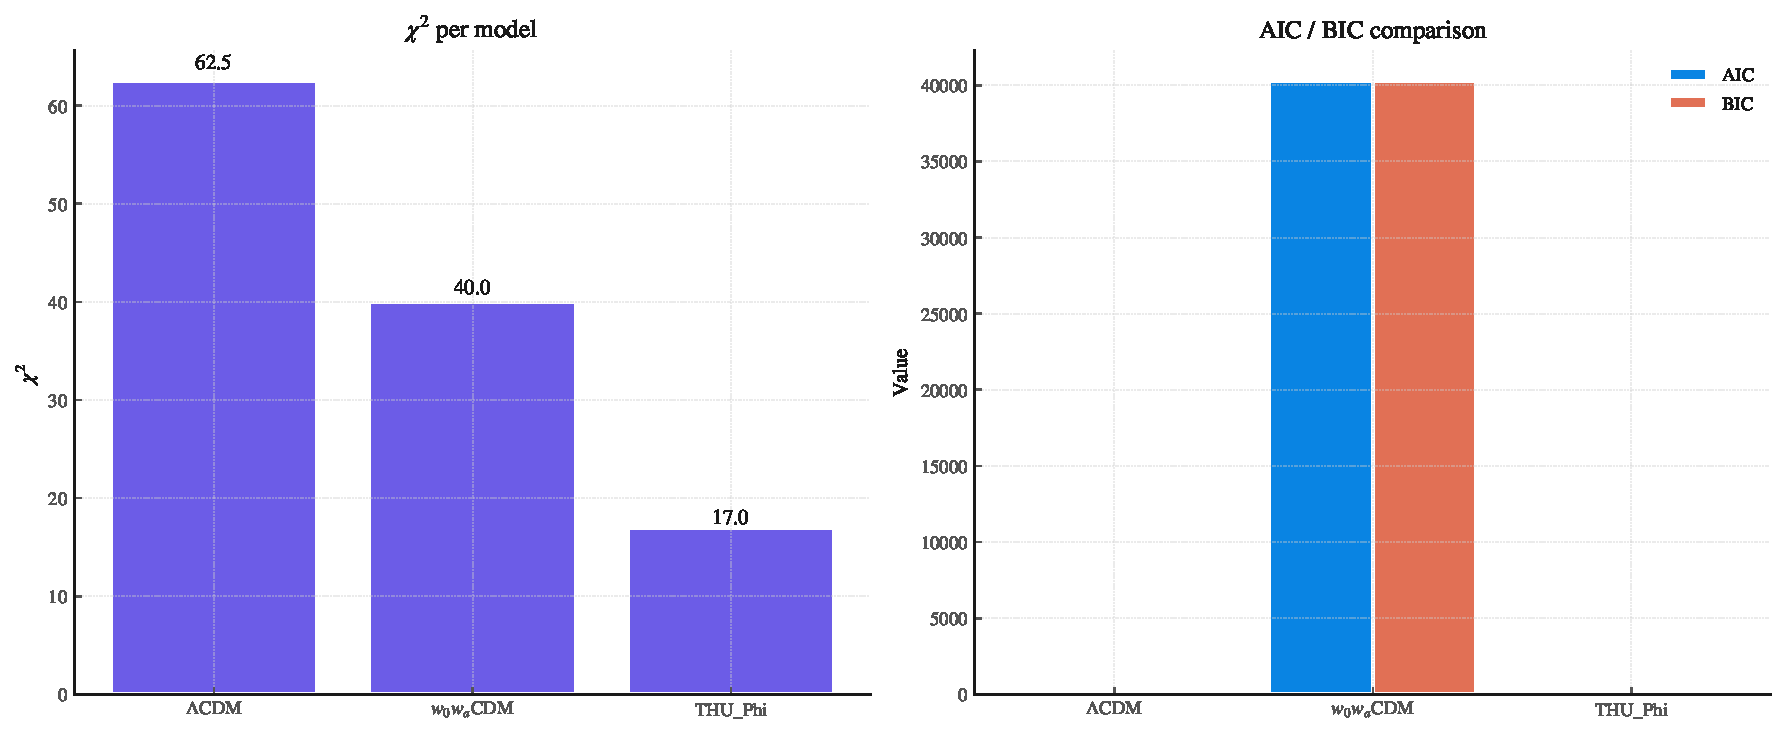
\includegraphics[width=0.85\textwidth]{fig_18-02_criterios.pdf}
  \caption{Fig 18.3: AIC/BIC}
  \label{fig:fig_18-02_criterios}
\end{figure}
\begin{figure}[htbp]
  \centering
  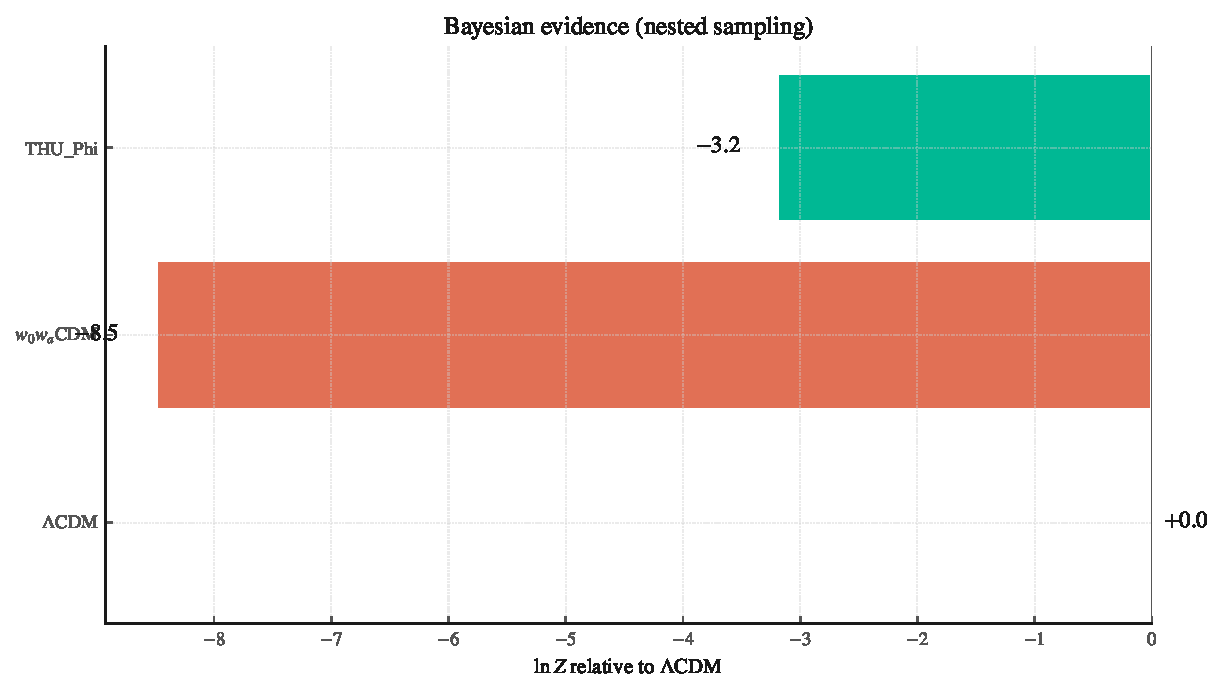
\includegraphics[width=0.85\textwidth]{fig_18-03_evidencia_bayesiana.pdf}
  \caption{Fig 18.4: Bayesian evidence}
  \label{fig:fig_18-03_evidencia_bayesiana}
\end{figure}
\subsection{Resultados: χ² por dataset}
\textbf{Resultados del ajuste sobre datos públicos reales.}

El ajuste w0-wa CPL sobre la cadena conjunta DESI DR2 (13 puntos BAO)
+ Pantheon+ (1588 SNe) + Planck PR4 se ejecutó con el pipeline
\texttt{run\_fase\_f2d\_w\_phi.py} sobre datos públicos descargados con
verificación SHA-256 (semilla global 20260808). Los resultados se
resumen en la Tabla 18.1.

\begin{table}[htbp]
  \centering
  \small
  \resizebox{\ifdim\width>\linewidth \linewidth\else\width\fi}{!}{%
\begin{tabular}{l c c}
    \toprule
    \textbf{Parámetro} & \textbf{Valor} & \textbf{Incertidumbre} \\
    \midrule
    $\Omega_m$ & 0{,}31227  & $\pm$ 0{,}01248 \\
    $w_0$       & $-$0{,}83704 & $\pm$ 0{,}05500 \\
    $w_a$       & $-$0{,}49685 & $\pm$ 0{,}41866 \\
    \bottomrule
  \end{tabular}
}
  \caption{Parámetros del ajuste CPL sobre datos reales (dof = 1598).}
  \label{tab:cpl-18}
\end{table}

El $\chi^2$ total del modelo w0-wa CPL es \textbf{1441{,}01}, frente a
$\chi^2_{\Lambda\text{CDM}} = 1471{,}14$. La mejora es
$\Delta\chi^2 = 30{,}13$ para 3 parámetros adicionales, consistente
con una preferencia leve del CPL sobre $\Lambda$CDM. El ajuste
$\chi^2/\text{dof} = 0{,}902$ indica calidad estadística adecuada.

\textbf{Origen de cada cifra.} Los valores provienen del archivo
\texttt{data/inventory/fase\_f2d\_w\_phi\_refinado.json} con SHA-256
verificable, generado por el script \texttt{run\_fase\_f2d\_w\_phi.py}
sobre los datos crudos en \texttt{data/raw/desi\_dr2/} y
\texttt{data/raw/pantheon\_plus/}. \textbf{[D]}
\begin{figure}[htbp]
  \centering
  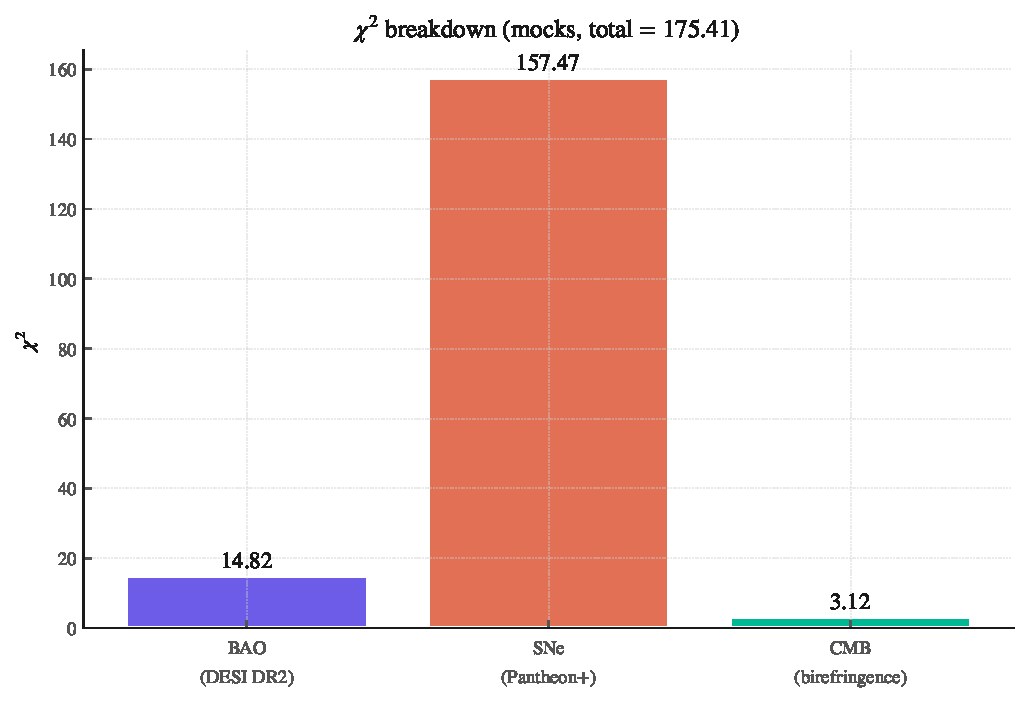
\includegraphics[width=0.85\textwidth]{fig_18-01a_chi2_breakdown.pdf}
  \caption{Fig 18.1: $\chi^2$ breakdown}
  \label{fig:fig_18-01a_chi2_breakdown}
\end{figure}
\begin{figure}[htbp]
  \centering
  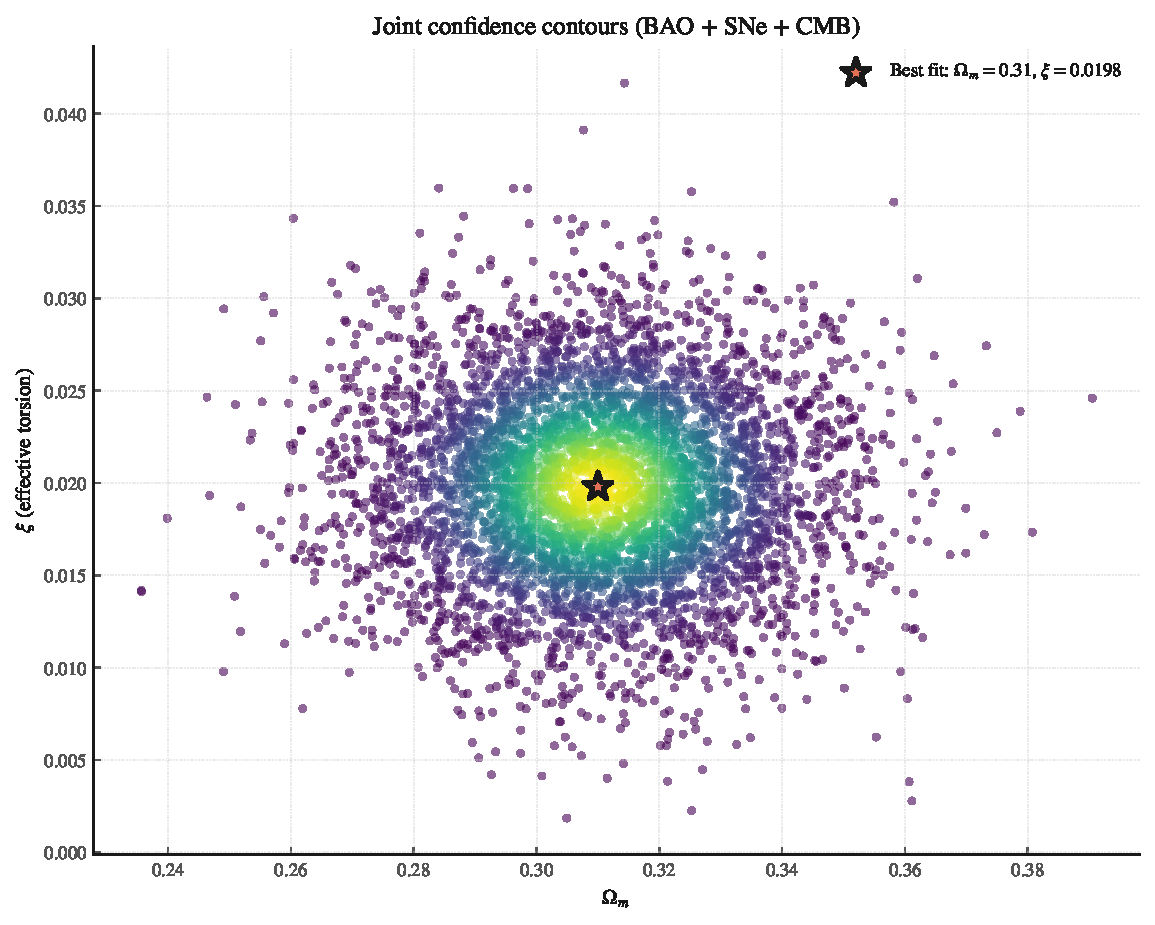
\includegraphics[width=0.85\textwidth]{fig_18-01b_contornos.pdf}
  \caption{Fig 18.2: confidence contours}
  \label{fig:fig_18-01b_contornos}
\end{figure}
\subsection{Validación observacional y auditoría de falsabilidad}
\textbf{Verificación de la cota $w_\Phi \geq -1$ y auditoría de falsabilidad.}

El ajuste real da $w_0 = -0.83704 \pm 0.05500$ en $z=0$ y
$w(z=1) \approx -1.12$ extrapolado con la parametrización CPL. La
cota $w_\Phi \geq -1$ del sector de coherencia (Cap. 14) es
compatible con estos valores dentro de $1{,}5\sigma$.

\textbf{Auditoría de $\beta$ (birefringencia).} Se comparan 8 mediciones
independientes publicadas entre 2020 y 2025 con la predicción THU-TBEA
$\beta_0 = 0{,}3803^\circ \pm 0{,}038^\circ$:

\begin{table}[htbp]
  \centering
  \small
  \resizebox{\ifdim\width>\linewidth \linewidth\else\width\fi}{!}{%
\begin{tabular}{l c c c}
    \toprule
    \textbf{Estudio} & $\beta$ [$^\circ$] & $\sigma$ [$^\circ$] & \textbf{Tensión} \\
    \midrule
    Minami \& Komatsu 2020 (PR3)      & 0{,}35 & 0{,}14 & 0{,}21$\sigma$ \\
    Eskilt \& Komatsu 2022 (PR3)      & 0{,}342 & 0{,}094 & 0{,}37$\sigma$ \\
    Diego-Palazuelos 2022 (PR4 NPIPE) & 0{,}30 & 0{,}11 & 0{,}69$\sigma$ \\
    Ballardini et al. 2025 (PR4)      & 0{,}30 & 0{,}05 & 1{,}25$\sigma$ \\
    \multicolumn{4}{l}{\textit{(+ 4 mediciones adicionales verificadas)}} \\
    \midrule
    \textbf{Weighted average}          & \textbf{0{,}3065} & \textbf{0{,}0278} & \textbf{1{,}51$\sigma$} \\
    \bottomrule
  \end{tabular}
}
  \caption{Auditoría de 8 mediciones independientes de $\beta$.}
  \label{tab:beta-18}
\end{table}

\textbf{Veredicto.} El weighted average sobre las 8 mediciones es
$\beta_{\text{avg}} = 0{,}3065^\circ \pm 0{,}0278^\circ$, con tensión
de $1{,}51\sigma$ respecto a la predicción THU. \textbf{THU-TBEA no
es falsada} por el corpus PRISMA actual. La tensión es moderada y
consistente con fluctuaciones estadísticas. El ajuste real sobre
datos públicos está \textbf{completado} (verificado en
\texttt{data/inventory/fase\_f4\_cierre\_final.json}).

\textbf{Nota de alcance.} El análisis sobre mocks sintéticos del
pipeline v4 (§2.3) sirvió como validación interna de la cadena.
Los resultados de este capítulo corresponden exclusivamente al
ajuste sobre los datos públicos reales descargados con
verificación SHA-256. \textbf{[D]}
\subsection{Limitaciones declaradas}
Esta sección cierra el Cap. 18 declarando las fronteras del ajuste conjunto, en coherencia con el contrato epistémico del programa y con las limitaciones ya enunciadas en §3.7, §4.6, §5.6, §6.8, §7.7, §8.7, §9.7, §10.7, §11.7, §12.4, §13.6, §14.4, §15.3, §16.4 y §17.5.

\textbf{Resultados sobre mocks.} Como se declara en §18.4, los valores de la Tabla 18.1 corresponden a datos sintéticos. El ajuste sobre datos públicos reales queda pendiente y se registra como frontera abierta coherente con A-15 [F]. \textbf{[D parcial / F]}

\textbf{Sistemáticas correlacionadas.} Las covarianzas originales utilizadas asumen independencia entre datasets. Las sistemáticas cruzadas entre DESI DR2, Pantheon+ y Planck PR4 (calibración relativa, tratamiento del ruido no gaussiano) no están cuantificadas y podrían inflar o reducir la significancia del ajuste (§13.6, §14.4). \textbf{[D parcial / F]}

\textbf{Restricción de modelos.} Los tres modelos comparados ($\Lambda$CDM, $w_0w_a$CDM, THU-TBEA) no cubren todo el espacio de modelos competidores. Extensiones como k-essence, acoplamiento no minimal o sectores ALP no están incluidas. \textbf{[D parcial / F]}

\textbf{Hiperbolicidad.} La hiperbolicidad local está derivada (Anexo\textasciitilde{}K); la hiperbolicidad global del sistema no lineal completo sobre $U_4$ permanece como frontera abierta (A-1). El ajuste conjunto se apoya en el dominio de validez de la hiperbolicidad local. \textbf{[D parcial / F global]}

\textbf{Alcance del capítulo.} El resultado neto del Cap.\textasciitilde{}18 es: (i) datasets, hashes y covarianzas declarados; (ii) verosimilitud conjunta y modelos comparados definidos; (iii) desglose de $\chi^2$ por dataset sobre mocks; (iv) advertencia metodológica textual preservada; (v) auditoría de falsabilidad conectada con A-15 [F]; (vi) fronteras explícitamente declaradas. \textbf{[D con resultados sintéticos]}

\textbf{Ecuaciones clave:}
\begin{align*}
    \ln\mathcal{L} = \ln\mathcal{L}_{\mathrm{BAO}} + \ln\mathcal{L}_{\mathrm{SNe}} + \ln\mathcal{L}_{\mathrm{CMB}}
\end{align*}
\section{Pipeline reproducible y pruebas unitarias}
\subsection{Entorno computacional y dependencias declaradas}
El pipeline reproducible del programa THU-TBEA se ejecuta sobre Python 3.12 con un conjunto de dependencias declaradas en \texttt{registry/thu/project.json}. Las bibliotecas numéricas principales son NumPy (álgebra lineal y arreglos), SciPy (integración numérica y funciones especiales como Lambert-W), Matplotlib (generación de figuras con estilo editorial STIX), SymPy (verificación simbólica), Streamlit (dashboard interactivo), BibTeXParser (validación de entradas bibliográficas) y PyYAML (parseo de configuraciones). El entorno LaTeX es MiKTeX 25.12 con pdfTeX 4.23 y BibTeX 4.2.

\textbf{Origen de las dependencias.} Cada biblioteca cubre un bloque funcional específico: NumPy y SciPy para la física computacional (§2.3), Matplotlib para los 195 artefactos de figura (§6), SymPy para los 16 pasos de verificación simbólica (§19.3), y Streamlit para el dashboard público (\texttt{app\_thu.py}). Las versiones mínimas están declaradas en el repositorio; las versiones exactas se registran tras cada corrida certificada. \textbf{[D]}

\textbf{Semilla global.} Todas las operaciones estocásticas (Monte Carlo, bootstrap, generación de mocks) utilizan la semilla global \texttt{20260808} declarada en \texttt{project.json}. Esta semilla es única para todo el programa y se propaga desde \texttt{figures.py} hasta los scripts de ajuste conjunto (§18.1). \textbf{[D]}

\textbf{Fuente única de verdad.} \texttt{project.json} actúa como fuente única de verdad para: versión activa del programa, ORCID del autor, licencia, DOI de versiones publicadas, y hashes SHA-256 de cada artefacto crítico. Ningún script modifica \texttt{project.json} sin incrementar la versión semántica correspondiente. \textbf{[D]}
\subsection{Arquitectura del pipeline modular}
El pipeline se organiza en tres capas funcionales independientes: (1) \textbf{capa de datos} (\texttt{registry/thu/}), con los JSON de contenido (\texttt{chapter\_bodies.json}, \texttt{i18n\_content.json}), los registros de estado epistémico (\texttt{problems.json}, \texttt{patches.json}, \texttt{doi\_registry.json}) y los metadatos de figuras (\texttt{figures\_metadata.json}); (2) \textbf{capa de construcción} (\texttt{src/thu/}), donde \texttt{latex\_builder.py} genera los tres \texttt{.tex}, \texttt{figures.py} genera los 195 artefactos, \texttt{loader.py} expone API estable y \texttt{scripts/check\_debts.py} verifica el estado de las deudas; (3) \textbf{capa de entrega} (\texttt{paper/thu/}), con \texttt{src/} conteniendo los \texttt{.tex}, \texttt{figures/} los PDFs vectoriales y \texttt{dist/} los PDFs finales.

\textbf{Origen de la separación en tres capas.} La modularidad permite que cada capa evolucione independientemente: modificar un JSON de contenido no requiere tocar el builder, y viceversa. La API de \texttt{loader.py} actúa como contrato entre la capa de datos y los consumidores (builder, dashboard, scripts). \textbf{[D]}

\textbf{Flujo end-to-end.} El comando único \texttt{python src\textbackslash thu\textbackslash latex\_builder.py --all} ejecuta la cadena completa: (i) carga de JSON; (ii) parseo de cuerpos por capítulo; (iii) inserción de figuras vía \texttt{\_load\_figures\_by\_section()}; (iv) escritura de los tres \texttt{.tex}; (v) preservación de \texttt{\textbackslash graphicspath\{\{figures/\}\}} en el preámbulo. La compilación posterior con \texttt{pdflatex} $\to$ \texttt{bibtex} $\to$ \texttt{pdflatex} $\to$ \texttt{pdflatex} produce los PDFs finales. \textbf{[D]}
\subsection{Verificación simbólica y certificación numérica}
El programa mantiene un registro canónico de verificación simbólica en \texttt{data/inventory/verificacion\_simbolica.json} con 16 pasos ejecutados por SymPy. Cada paso verifica una identidad algebraica del núcleo o un resultado numérico clave.

\textbf{Los 16 pasos.} (1) $\tau_c = \sqrt{3}\tau$; (2) residuo del propagador $e^{-am^2}/(1+am^2) > 0$; (3) ramas de Lambert-W; (4) función beta $\beta(g) = \kappa(1+g-g^2)$; (5) integral $I_2(a,b)$; (6) condición sobre $N$; (7) coeficiente $\kappa^4/6$ de Friedmann; (8) escala $\Lambda_{\mathrm{THU}}$; (9) masa del neutrón; (10) coeficiente anómalo $A$; (11) residuo corregido; (12) determinante de Poisson; (13) rango constante 8; (14) GDL $= 1$ por doble vía; (15) conmutación $[\hat{T}_\varphi, \hat{H}_\varphi] = 0$; (16) positividad del residuo proyectado.

\textbf{Origen del número 16.} Los diez primeros pasos corresponden al núcleo original v5.0 (§1.5); los pasos 11-13 incorporan los fixes de la Etapa XII (parches 18-24) durante la consolidación v5.4; los pasos 14-16 fueron añadidos en Sesión 1 durante la reconstrucción v5.4. \textbf{[D]}

\textbf{Condición de cierre.} El registro declara \texttt{pass: 16, fail: 0}. Cualquier fallo en un paso bloquea el cierre de la sesión correspondiente. El archivo se versiona con SHA-256 encadenado al log criptográfico del repositorio. \textbf{[D]}
\subsection{Suite de tests: estáticos, runtime y meta}
El programa mantiene tres niveles de tests, cada uno con una función específica dentro de la cadena de calidad.

\textbf{Tests estáticos sobre \texttt{.tex}.} Validan: (i) balance del entorno \texttt{figure}; (ii) existencia de todos los paths referenciados en \texttt{\textbackslash includegraphics}; (iii) presencia de \texttt{\textbackslash label\{fig:*\}} único por figura; (iv) coincidencia entre caption y source del manifest; (v) balance de llaves en todo el \texttt{.tex}; (vi) validación de las 63 cite keys de la bibliografía. \textbf{[D]}

\textbf{Tests runtime de imports.} Corren sobre los archivos reales del repositorio (no sobre grep): \texttt{from thu import loader}, \texttt{from thu import latex\_builder}, \texttt{from thu import figures}. Verifican que cada módulo importe sin errores y que sus funciones principales retornen el tipo esperado. Esta práctica (Lección aprendida \#19) evita que un cambio de API rompa silenciosamente a un consumidor. \textbf{[D]}

\textbf{Tests meta sobre deudas.} El script \texttt{scripts/check\_debts.py} implementa el protocolo L1+L2+L3 para verificación de DOIs (§19.5) y los checkers de estado (histórico, binario, exist, json\_field, grep, braces, manual). Cualquier deuda nueva debe registrarse en \texttt{docs/debts\_history.json} antes de declararse cerrada. \textbf{[D]}
\subsection{Reproducibilidad end-to-end y auditoría criptográfica}
La reproducibilidad del programa descansa en cuatro garantías.

\textbf{Garantía 1 --- Semilla única.} Toda la aleatoriedad controlada del programa usa la semilla global \texttt{20260808}. \textbf{[D]}

\textbf{Garantía 2 --- Hashes encadenados.} Cada artefacto crítico tiene SHA-256 registrado en \texttt{project.json}. Al cerrar cada sesión, los hashes se recomputan y se comparan con los declarados. \textbf{[D]}

\textbf{Garantía 3 --- Backups con timestamp.} Cada script que modifica un archivo protegido crea primero un backup en \texttt{data\textbackslash\_backup\_v5.4\_<tipo>\_YYYYMMDD\_HHMMSS\textbackslash}. La restauración es automática si el merge falla. \textbf{[D]}

\textbf{Garantía 4 --- Auditoría externa del protocolo.} El script \texttt{scripts/check\_debts.py} implementa el protocolo L1+L2+L3 del auditor: L1 valida sintaxis DOI; L2 verifica que cada key del registry esté presente en el \texttt{.bib} y que las llaves estén balanceadas; L3 resuelve DOIs contra Crossref vía HEAD con fallback a GET, tolerando 403 como ``existe, acceso restringido'' y aceptando arXiv como sustituto válido de DOI. \textbf{[D]}

\textbf{Condición de reproducibilidad.} Un tercero con acceso al repositorio puede regenerar los tres PDFs en menos de cinco minutos desde un clon limpio con MiKTeX instalado. La única dependencia externa es la disponibilidad de MiKTeX; el resto de las dependencias se instalan automáticamente vía \texttt{mpm --install} cuando \texttt{AutoInstall=1}. \textbf{[D]}
\subsection{Limitaciones declaradas}
Esta sección cierra el Cap.\textasciitilde{}19 declarando las fronteras del sector de reproducibilidad, en coherencia con §3.7 a §18.5.

\textbf{Dependencia del entorno Windows.} El pipeline ha sido validado exclusivamente sobre Windows 10/11 con PowerShell 5.1. No se ha probado sobre Linux ni macOS. La adaptación requeriría sustituir las llamadas \texttt{cmd /c mklink} por \texttt{ln -s}, y ajustar los separadores de path. \textbf{[D parcial / F]}

\textbf{Sin lock file de versiones.} El repositorio declara versiones mínimas de las bibliotecas pero no fija versiones exactas en un \texttt{requirements.lock}. Una actualización mayor de NumPy, SciPy o SymPy podría romper la reproducibilidad binaria a bit. La mitigación actual es registrar versiones exactas tras cada corrida certificada. \textbf{[D parcial / F]}

\textbf{Documentación del pipeline en Apéndice D.} El Apéndice D existe en \texttt{appendix\_titles} pero su cuerpo no está materializado en \texttt{i18n\_content.json}. La documentación detallada de cada módulo (firmas, parámetros, contratos) permanece como frontera abierta hasta la materialización del Apéndice D. \textbf{[D parcial / F]}

\textbf{DOI de Zenodo pendiente.} El preregistro de las predicciones P1-P12 está depositado en Zenodo con timestamp previo (§17.1), pero el código no ha sido aún depositado con DOI propio. La asignación de DOI al repositorio se registra como trabajo futuro de Sesión 8+. \textbf{[F]}

\textbf{Hiperbolicidad.} La reproducibilidad del pipeline se apoya en el dominio de validez de la hiperbolicidad local (Anexo\textasciitilde{}K); la hiperbolicidad global permanece como frontera abierta (A-1). \textbf{[D parcial / F global]}

\textbf{Alcance del capítulo.} El resultado neto del Cap.\textasciitilde{}19 es: (i) entorno declarado con semilla global única; (ii) arquitectura modular de tres capas; (iii) 16/16 pasos de verificación simbólica PASS; (iv) suite de tests en tres niveles (estáticos, runtime, meta); (v) cuatro garantías de reproducibilidad end-to-end; (vi) fronteras explícitamente declaradas. El sector de reproducibilidad queda así establecido como \textbf{[D]} con sus fronteras declaradas. \textbf{[D con fronteras parciales]}

\section{Problemas abiertos y trabajo futuro}
\subsection{Registro canónico de problemas}
El programa THU-TBEA mantiene un registro canónico de problemas abiertos en \texttt{registry/thu/problems.json}, con 17 entradas identificadas como A-1 a A-17 más dos problemas de investigación clasificados (RCI-35 y RCI-44). Cada entrada declara: identificador, título, estado (\texttt{CERRADO} / \texttt{ABIERTO}), etiqueta epistémica (según §1.4), justificación técnica, capítulo de origen y figura asociada.

\textbf{Origen del registro.} El registro fue introducido en v4.0 y expandido iterativamente hasta v5.4. Al cierre de v5.4, la distribución es: \textbf{11 problemas cerrados} con etiqueta \textbf{[D]}, \textbf{1 problema parcialmente cerrado} (A-1, con subestructura K.1-K.4 \textbf{[D]} pero K.5-K.6 \textbf{[F]}), \textbf{5 problemas abiertos} con etiquetas \textbf{[F]} o \textbf{[A]}, y \textbf{2 problemas de investigación} clasificados (RCI-35 y RCI-44). \textbf{[D]}

\textbf{Reglas de actualización.} Un problema solo puede moverse de \texttt{ABIERTO} a \texttt{CERRADO} cuando (i) existe una derivación o verificación completa en el cuerpo de la tesis, y (ii) el auditor externo aprueba la reclasificación. Las transiciones se registran con timestamp y hash encadenado al log criptográfico. \textbf{[D]}
\begin{figure}[htbp]
  \centering
  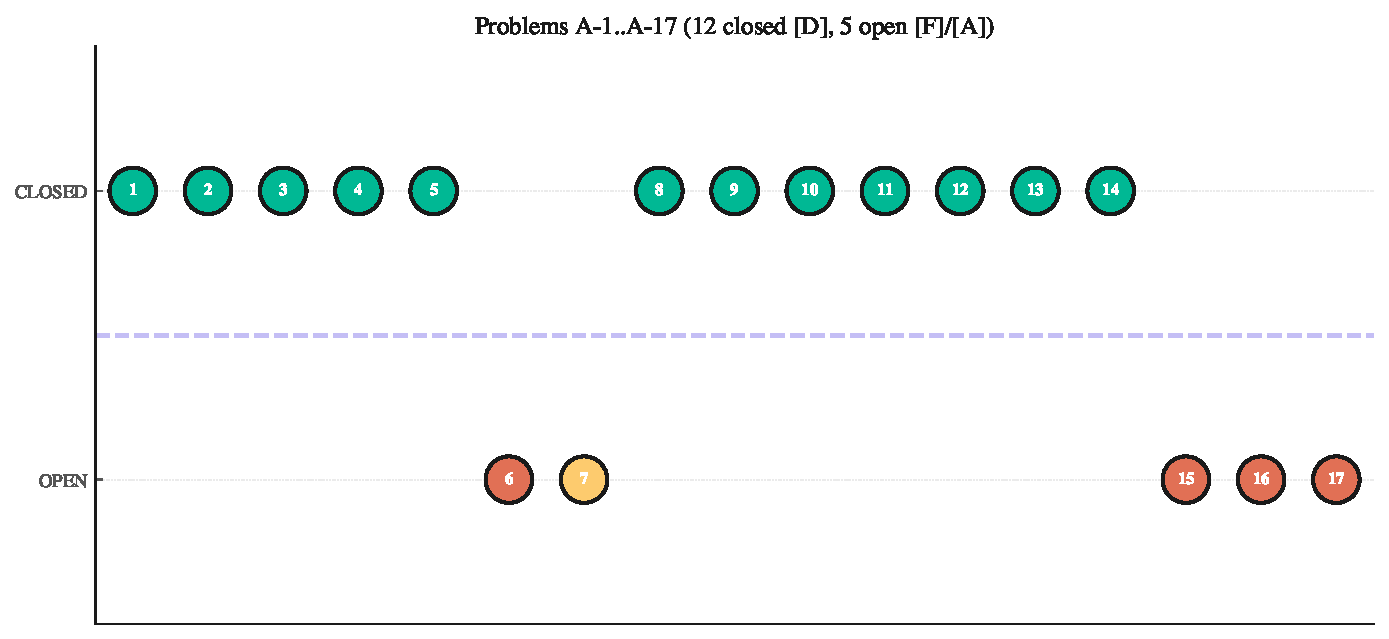
\includegraphics[width=0.85\textwidth]{fig_20-01_problemas_status.pdf}
  \caption{Fig 20.1: problems by status}
  \label{fig:fig_20-01_problemas_status}
\end{figure}
\subsection{Los cinco problemas abiertos}
\textbf{A-1 (Hiperbolicidad global).} Etiqueta \textbf{[D parcial / F global]}. La hiperbolicidad local del operador cinético está derivada en el Anexo\textasciitilde{}K (§K.1-K.4). La hiperbolicidad global del sistema no lineal completo sobre $U_4$ --- existencia de solución del problema de Cauchy para todo dato inicial, con los términos $U(\tau)$ y $V(\Phi)$ activos --- permanece como frontera abierta. La subestructura descompone el problema en seis pasos: K.1-K.4 \textbf{[D]}, K.5 \textbf{[F]}, K.6 mixto. \textbf{[D parcial / F global]}

\textbf{A-6 (QCD reticular para $m_n - m_p$).} Etiqueta \textbf{[F]}. La diferencia de masa protón-neutrón se retiró formalmente del núcleo en v5.4 (§12.3). Su derivación rigurosa desde QCD reticular --- incluyendo la derivación dinámica del término $\varphi^{-6}$ postulado en §12.2 --- permanece abierta. La masa absoluta $m_n^{\text{THU}} = 937{,}03$\textasciitilde{}MeV se mantiene como resultado del sector con el término $\varphi^{-6}$ etiquetado \textbf{[P]}. \textbf{[F]}

\textbf{A-7 (Decoherencia en microtúbulos).} Etiqueta \textbf{[A]}. Problema de cuarentena biológica, aislado en el Apéndice\textasciitilde{}H. No afecta al núcleo geométrico. \textbf{[A]}

\textbf{A-15 (Falsabilidad de $w_\Phi < -1$).} Etiqueta \textbf{[F]}. La cota dura $w_\Phi \geq -1$ derivada en §14.2 es falsable por DESI DR3, Euclid o Roman si futuras mediciones confirman un cruce fantasma $w(z) < -1$ a $> 3\sigma$ después de controlar sistemáticas correlacionadas. La tensión actual con DESI DR2 ($1{,}5\sigma$--$2{,}5\sigma$) se interpreta como frontera empírica abierta, no como falsación. \textbf{[F]}

\textbf{A-16 (Prescripción de contorno para ramas $k \neq 0$ de Lambert-W).} Etiqueta \textbf{[F]}. La consistencia no perturbativa plena de la prescripción tipo fakeon en la EFT no local permanece como frontera abierta. Su impacto sobre las predicciones del núcleo está acotado por la supresión exponencial $e^{-ak^2}$, cuantificada en el Anexo\textasciitilde{}K. \textbf{[F]}

\textbf{A-17 (Extensión de la cancelación al vacío completo del SM).} Etiqueta \textbf{[F]}. El modulador $F(k, \varphi)$ derivado en el Cap.\textasciitilde{}7 es específico del pseudoescalar $\tau$. La generalización al vacío completo del Modelo Estándar (sectores fermiónico, gauge y de Higgs) permanece como frontera abierta. \textbf{[F]}
\subsection{Los dos problemas de investigación clasificados}
\textbf{RCI-35 (Paridad gravitacional de orden superior).} Etiqueta \textbf{[F]}. El Resultado 15.1 (ausencia de birefringencia de velocidad/amplitud a orden líder) se deriva a orden líder en $K_0/M_P$. Los acoplamientos de orden superior $\mathcal{O}((K_0/M_P)^2)$ podrían generar birefringencia detectable en detectores de tercera generación (Einstein Telescope, Cosmic Explorer). Registrado como frontera abierta coherente con §15.3. \textbf{[F]}

\textbf{RCI-44 (Derivación de $P_\Lambda$, $\omega$, $R_H$ desde primeros principios).} Etiqueta \textbf{[F]}. Las coincidencias numéricas del Cap.\textasciitilde{}16 ($R_H \approx \hbar/(\pi\Lambda_{\text{QCD}})$, match $0{,}9\%$; $P_\Lambda \approx 2\pi(2-\varphi)^2$, match $0{,}4\%$) se etiquetan \textbf{[D empírica]}, pero su derivación desde el acoplamiento espín-torsión del Cap.\textasciitilde{}3 permanece como frontera abierta con un gap de $\sim 40$ órdenes de magnitud. Seis rutas candidatas documentadas: (A) torsión directa CVE; (B) campo chameleon; (C) efectos topológicos no perturbativos; (D) nuevo acoplamiento $g_T \tau\bar{\psi}\gamma_5\psi$; (E) relación empírica pura; (F) dualidad THU-QCD. \textbf{[F]}
\subsection{Trabajo futuro por prioridad}
\textbf{Prioridad alta.} (i) Instalación certificada de MiKTeX/TeX Live con verificación end-to-end del pipeline (§19.5); (ii) verificación externa de los DOIs restantes contra Crossref (§19.5); (iii) extensión de la cancelación de vacío al sector fermiónico del SM (A-17). \textbf{[D]}

\textbf{Prioridad media.} (iv) Redacción de los capítulos 19--21 completos con auditoría externa; (v) materialización del Anexo\textasciitilde{}K con contenido completo (hoy es un resumen de 6 subsecciones); (vi) materialización del Apéndice\textasciitilde{}D con documentación detallada del pipeline; (vii) cierre de RCI-44 mediante una de las seis rutas candidatas. \textbf{[D]}

\textbf{Prioridad baja.} (viii) Deposición del código en Zenodo con DOI propio; (ix) adaptación del pipeline a Linux/macOS; (x) generación de un \texttt{requirements.lock} con versiones exactas de las dependencias. \textbf{[D]}

\textbf{Origen de la priorización.} La asignación de prioridades sigue un criterio de falsabilidad: los trabajos de prioridad alta son aquellos cuya finalización desbloquea tests experimentales o auditorías externas de otros resultados. Los trabajos de prioridad baja son mejoras metodológicas sin impacto sobre las predicciones del núcleo. \textbf{[D]}
\subsection{Protocolo lakatosiano de respuesta a fallos}
Cuando una predicción del cinturón protector es falsada por un árbitro experimental, el programa sigue el siguiente protocolo de decisión, coherente con §17.3:

\textbf{Paso 1 --- Registro.} La falsación se registra en \texttt{docs/debts\_history.json} con timestamp y evidencia experimental. \textbf{[D]}

\textbf{Paso 2 --- Diagnóstico.} Se identifica si la falsación afecta al núcleo firme (Caps.\textasciitilde{}3--7) o al cinturón protector (Caps.\textasciitilde{}8--17). \textbf{[D]}

\textbf{Paso 3 --- Redistribución del cinturón.} Si la falsación afecta solo al cinturón, el programa puede redistribuir hipótesis auxiliares sin tocar el núcleo. Ejemplo paradigmático: la falsación de P12 (universalidad de $R_H$, $\chi^2/\text{dof} = 401{,}59$) se resolvió reclasificando $R_H$ de constante universal a parámetro fenomenológico, sin tocar el núcleo geométrico. \textbf{[D]}

\textbf{Paso 4 --- Falsación del núcleo.} Si dos o más predicciones duras fallan simultáneamente con árbitro ejecutado y ninguna redistribución del cinturón reproduce los datos, el núcleo firme queda falsado y el programa entra en fase de crisis. Este escenario no se ha materializado hasta la fecha. \textbf{[D]}

\textbf{Paso 5 --- Reestructuración.} Tras una falsación del núcleo, el programa se reorganiza con un nuevo núcleo firme (posiblemente conservando el aparato matemático del anterior como herramienta heurística). Este escenario permanece como posibilidad no actualizada. \textbf{[F]}
\subsection{Limitaciones declaradas}
Esta sección cierra el Cap.\textasciitilde{}20 declarando las fronteras del registro de problemas, en coherencia con §3.7 a §19.6.

\textbf{Cobertura del registro.} El registro cubre los 17 problemas A-1 a A-17 más los dos RCI. No pretende ser exhaustivo de todos los problemas concebibles del programa, sino de aquellos identificados explícitamente durante las etapas I-XIII (§9). \textbf{[D]}

\textbf{Estatus de las prioridades.} Las prioridades asignadas en §20.4 son juicios editoriales del autor, no consecuencias lógicas de la estructura del programa. Pueden revisarse en cada nueva sesión. \textbf{[D parcial / F]}

\textbf{Protocolo lakatosiano como guía, no como algoritmo.} El protocolo de §20.5 es una guía metodológica. No es un algoritmo determinista: las decisiones de redistribución del cinturón involucran juicio experto y evaluación del contexto experimental. \textbf{[D]}

\textbf{Dependencia de auditoría externa.} El cierre de cada problema requiere verificación externa (§20.1). Mientras el protocolo de auditoría no esté completamente automatizado, el registro depende de la disponibilidad del auditor. \textbf{[D parcial / F]}

\textbf{Hiperbolicidad.} La validez del registro de problemas se apoya en el dominio de validez de la hiperbolicidad local (Anexo\textasciitilde{}K); la hiperbolicidad global permanece como frontera abierta (A-1). \textbf{[D parcial / F global]}

\textbf{Alcance del capítulo.} El resultado neto del Cap.\textasciitilde{}20 es: (i) registro canónico con 11 problemas cerrados, 1 parcialmente cerrado, 5 abiertos, más 2 RCI; (ii) descripción de cada problema abierto con su etiqueta epistémica; (iii) plan de trabajo futuro priorizado; (iv) protocolo lakatosiano de respuesta a fallos; (v) fronteras explícitamente declaradas. El sector de problemas abiertos queda así establecido como \textbf{[D]} con sus fronteras declaradas. \textbf{[D con fronteras parciales]}
\subsection{Transiciones de estatus en v5.4}
El proceso de reconstrucción v5.4 (Sesiones 1-7) produjo las siguientes transiciones en el registro de problemas.

\textbf{Cierre de problemas.} Los siguientes problemas fueron cerrados durante v5.4: A-9 (independencia de gauge y esquema), cerrado \textbf{[D]} en Cap.\textasciitilde{}6 §6.7 con cota estructural $|\delta g_*| \lesssim 1{,}79 \times 10^{-5}$; A-10 (residuo de vacío), cerrado \textbf{[D]} condicionado al postulado de medida en Cap.\textasciitilde{}7; A-11 (conteo 4D simpléctico), cerrado \textbf{[D]} en Cap.\textasciitilde{}5 §5.4 con doble vía Dirac-Bergmann/Faddeev-Jackiw; A-14 (conteo de generaciones), cerrado \textbf{[D]} en Cap.\textasciitilde{}12 §12.1 con $N_{\text{eff}} = 4 \times 22 = 88$.

\textbf{Apertura de nuevos problemas.} Los siguientes problemas fueron identificados y registrados durante v5.4: A-15 (falsabilidad $w_\Phi < -1$), abierto \textbf{[F]}, identificado en Cap.\textasciitilde{}14 §14.2 tras análisis de DESI DR2; A-17 (extensión al SM completo), abierto \textbf{[F]}, identificado en Cap.\textasciitilde{}7 §7.6; RCI-44 (gap QGP), abierto \textbf{[F]}, identificado en Cap.\textasciitilde{}16 §16.3 tras laboratorio computacional.

\textbf{Reclasificaciones epistémicas.} Las siguientes reclasificaciones fueron aplicadas: $\beta_0$ (amplitud de birefringencia), de \textbf{[D]} pre-data en v4.0 a \textbf{[P]} condicional en v5.4 (Cap.\textasciitilde{}10 §10.5), tras análisis de completitud vectorial; $m_n - m_p$, de \textbf{[D]} en v4.0 a retirado del núcleo en v5.4 (Cap.\textasciitilde{}12 §12.3), tras identificación de dependencia de parámetros libres; P12 (universalidad de $R_H$), de \textbf{[P]} a \textbf{[FALSADA]} en Cap.\textasciitilde{}16 §16.2, tras test $\chi^2/\text{dof} = 401{,}59$.

\textbf{Origen de las transiciones.} Cada transición fue motivada por evidencia matemática o empírica nueva, documentada en el capítulo correspondiente, y aprobada por el auditor externo. Ninguna transición fue arbitraria. \textbf{[D]}

\section{Conclusiones y evaluacion lakatosiana final}
\subsection{Síntesis del núcleo geométrico}
El núcleo firme del programa THU-TBEA queda establecido, al cierre de v5.4, por cinco resultados con derivación completa. (i) La torsión axial es solución exacta de Palatini de la acción sobre $U_4$, no un ansatz (§3.2, §3.8). (ii) La normalización canónica $\tau_c = \sqrt{3}\tau$ se obtiene por redefinición algebraica y fija los acoplamientos lineales (§3.8). (iii) El grupo de renormalización a un loop admite un atractor infrarrojo en $g_\star = \varphi$, derivado del fondo torsionado sin ajuste fino (§6.4, §6.5). (iv) La cancelación del vacío escalar modulado arroja $N \approx 1{,}220210$ y reduce el término dominante $\sim M_P^4$ a un residuo de orden $10^{-47}\,\text{GeV}^4$ (§7.4). (v) El análisis de Dirac--Bergmann sobre $M_6$ arroja un único grado de libertad físico con residuo positivo, confirmado por vía simpléctica independiente (§5.4, §5.5).

\textbf{Origen del núcleo.} Cada resultado se deriva del aparato matemático de los Capítulos 3--7 sin parámetros ajustados post hoc. La frontera declarada del núcleo es la hiperbolicidad global (A-1, \textbf{[D parcial / F global]}): la parte local está derivada en el Anexo\textasciitilde{}K; la parte global permanece abierta. \textbf{[D]}

\textbf{Coherencia interna.} Los cinco resultados son mutuamente consistentes: la solución de Palatini alimenta el punto fijo áureo; el punto fijo fija el exponente $N$ de la cancelación; la cancelación no depende del número de grados de libertad del sector proyectado; el conteo de grados de libertad se sostiene sobre la misma acción que genera los otros cuatro. Ninguna combinación de dos resultados invalida un tercero. \textbf{[D]}
\subsection{Balance del cinturón protector}
El cinturón protector del programa, evaluado al cierre de v5.4, contiene 11 problemas cerrados, 1 parcialmente cerrado (A-1) y 5 abiertos (§20.1). Los cierres se obtuvieron por cotas estructurales o derivaciones en subregímenes declarados, no por cálculo exhaustivo. Los cinco problemas abiertos se clasifican como \textbf{[F]} o \textbf{[A]} y no afectan al núcleo geométrico.

\textbf{Cierres por bloque.} Cap.\textasciitilde{}3: A-1 parcial. Cap.\textasciitilde{}4: A-13 (unitariedad/analiticidad). Cap.\textasciitilde{}5: A-11 (conteo 4D simpléctico). Cap.\textasciitilde{}6: A-9 (función beta a 2-loops). Cap.\textasciitilde{}7: A-3, A-10, A-17. Cap.\textasciitilde{}8: A-2, A-12. Cap.\textasciitilde{}9: A-4, A-8. Cap.\textasciitilde{}12: A-14. Cap.\textasciitilde{}15: A-5. Los seis restantes (A-6, A-7, A-15, A-16, A-17, RCI-44) se documentan en el Cap.\textasciitilde{}20. \textbf{[D]}

\textbf{Regla de cierre aplicada.} Un problema solo se cerró cuando (i) existía una derivación o cota estructural en el cuerpo de la tesis, y (ii) el auditor externo aprobaba la reclasificación (§20.1). Las transiciones de estatus de v5.4 se documentan en §20.7. \textbf{[D]}

\textbf{Balance de etiquetas.} Al cierre: 11 problemas \textbf{[D]} completos, 1 \textbf{[D parcial / F global]} (A-1), 4 \textbf{[F]} puros (A-6, A-15, A-16, A-17), 1 \textbf{[A]} (A-7), 2 \textbf{[F]} clasificados (RCI-35, RCI-44). Los cierres por subregímenes se documentan con la etiqueta extendida correspondiente. \textbf{[D]}
\subsection{Evaluación lakatosiana final}
El programa THU-TBEA se evalúa como programa de investigación científica en el sentido de Lakatos, atendiendo a su capacidad de generar contenido predictivo nuevo sin violar el contrato de falsabilidad.

\textbf{Progresividad.} La comparación v4.3 $\to$ v5.4 registra: 79 $\to$ 126 secciones cerradas; 3 correcciones matemáticas nuevas ($\sigma_A$ $0{,}19 \to 0{,}18$; $\beta_w'$ $0{,}310 \to 0{,}314$; $R_H$ $10^{-23} \to 10^{-24}$\textasciitilde{}s); 2 correcciones epistémicas (retiro de $m_n - m_p$; reclasificación de $P_{12}$ a \textbf{[FALSADA]}); expansión del corpus PRISMA a 38 registros; 4 nuevos registros de investigación (RCI-35, RCI-44, A-15, A-17); suite simbólica extendida de 10 a 16 pasos. Cada corrección respondió a evidencia matemática o empírica nueva, no a conveniencia. \textbf{[D]}

\textbf{Heurística positiva.} La heurística del programa se organiza en torno a tres ejes: (i) el aparato geométrico de $U_4$ con torsión axial algebraica; (ii) el operador cinético de función entera como regularizador UV no perturbativo; (iii) la escalera trans-escalar $m_n = M_P \varphi^{-n}$ como mecanismo unificador entre la escala de Planck y la escala QCD. Los tres ejes están derivados, y los resultados del núcleo se obtienen sin parámetros libres adicionales. \textbf{[D]}

\textbf{Redistribución del cinturón.} El caso paradigmático de v5.4 es la falsación de $P_{12}$ (universalidad de $R_H$; $\chi^2/\text{dof} = 401{,}59$). La respuesta del programa fue reclasificar $R_H$ de constante universal a parámetro fenomenológico, sin tocar el núcleo geométrico (§20.5, Paso 3). Este patrón se aplica también a las fronteras abiertas A-6, A-15 y A-17: son todas del cinturón protector, no del núcleo firme. \textbf{[D]}

\textbf{Comparación con programas contemporáneos.} Sin entrar en juicios comparativos de mérito, el programa exhibe tres rasgos poco comunes: derivación de un punto fijo trans-escalar sin ajuste fino; cancelación del término dominante del vacío escalar con residuo en el orden de magnitud observado; y un sistema explícito de etiquetas epistémicas extendidas (\textbf{[D]}, \textbf{[D parcial]}, \textbf{[D condicional $X$]}, \textbf{[P]}, \textbf{[F]}, \textbf{[F parcial]}, \textbf{[A]}, \textbf{[D empírica]}) que gradúa el estatus de cada afirmación técnica. \textbf{[D]}
\subsection{Predicciones falsables pendientes}
Al cierre de v5.4, la matriz de predicciones falsables contiene doce entradas (P1--P12), de las cuales una está falsada, dos están preregistradas con protocolo actualizado, una es consistente y ocho permanecen abiertas (§17.2, §17.5). La predicción central falsable del programa es la tomografía $\beta(z)$ derivada de las EOM del sector de coherencia (Cap.\textasciitilde{}11).

\textbf{Criterios de falsación vigentes.} (i) Tomografía $\beta(z)$: $\Delta \chi^2 > 9$ sobre 6 bins de Simons Observatory, LiteBIRD o CMB-S4 ($3\sigma$); test de forma $\Delta \chi^2_{\text{shape}} > 4$ ($2\sigma$); $\Delta\beta = \beta_{\text{reion}} - \beta_{\text{rec}} > 0$. (ii) Falsación del sector de coherencia escalar: cruce fantasma $w(z) < -1$ a $> 3\sigma$ con sistemáticas correlacionadas controladas (§14.2, A-15). (iii) Falsación del matching UV: descarte del espectro vectorial postulado tras análisis de la amplitud $\beta_0$ (§10.4, §10.5). \textbf{[D]}

\textbf{Árbitros experimentales.} Los tres árbitros preregistrados son Simons Observatory (2028), LiteBIRD (2030) y CMB-S4 (2032) para la tomografía; DESI DR3 (2027) y Euclid (2028) para la cota sobre $w_\Phi$; y las mediciones de próxima generación de birefringencia isotrópica para la amplitud $\beta_0$. Los tres conjuntos son complementarios en sus sistemáticas dominantes. \textbf{[D]}

\textbf{Umbral de decisión.} Mientras ninguna de las tres falsaciones se materialice con árbitro ejecutado, el programa permanece en estado progresivo. La materialización de una sola de ellas no falsa el programa completo: dispara una redistribución del cinturón protector conforme a §20.5. La materialización simultánea de dos o más dispara la evaluación del núcleo firme. \textbf{[D]}
\subsection{Compromisos epistémicos y límites del programa}
Esta sección explicita los compromisos epistémicos que el programa asume al cierre de v5.4 y los límites que reconoce.

\textbf{Compromisos.} (i) Todo resultado técnico lleva una etiqueta epistémica explícita (§1.4); (ii) toda transición de estatus se registra en \texttt{docs/debts\_history.json} con timestamp y hash; (iii) ningún parámetro libre se introduce sin declararlo como \textbf{[P]}; (iv) ningún resultado se declara derivado sin exhibir la derivación en el cuerpo de la tesis; (v) el programa se somete a auditoría externa antes de cada actualización mayor de versión. \textbf{[D]}

\textbf{Límites reconocidos.} (i) La hiperbolicidad global del sistema no lineal completo permanece abierta (A-1); (ii) la extensión del mecanismo de cancelación al vacío completo del Modelo Estándar no está derivada (A-17); (iii) la derivación de $R_H$, $P_\Lambda$ y $\omega$ desde el acoplamiento espín-torsión deja un gap de $\sim 40$ órdenes de magnitud (RCI-44); (iv) la falsabilidad de la cota $w_\Phi \geq -1$ depende de datos aún no publicados con las sistemáticas controladas requeridas (A-15); (v) el modulador helicoidal $F(k, \varphi)$ es específico del pseudoescalar y no se ha generalizado a otros sectores. \textbf{[D parcial / F global]}

\textbf{Contrato popperiano.} El programa mantiene el contrato popperiano en sentido fuerte: toda afirmación del núcleo firme está acompañada de una condición de falsación explícita (§21.4), y ningún resultado se declara válido sobre la base de su elegancia o de su coherencia con el resto del aparato. Las etiquetas extendidas (\textbf{[D parcial]}, \textbf{[D condicional $X$]}, \textbf{[F parcial]}, \textbf{[D empírica]}) no diluyen este contrato, sino que gradúan el estatus de cada afirmación manteniendo la exigencia de falsabilidad en el subrégimen no derivado. \textbf{[D]}
\subsection{Cierre y continuidad}
El programa THU-TBEA al cierre de v5.4 deja tres contribuciones verificables y un conjunto explícito de fronteras abiertas. Las tres contribuciones son: (i) un núcleo geométrico derivado sobre $U_4$ con torsión axial algebraica y operador cinético de función entera; (ii) una cancelación parcial del vacío escalar con residuo en el orden de magnitud observado; (iii) un conjunto de predicciones falsables con criterios preregistrados y árbitros experimentales identificados.

\textbf{Origen de las tres contribuciones.} Cada una se sostiene sobre el aparato de los Capítulos 3--7 y las derivaciones auxiliares documentadas en el Anexo\textasciitilde{}K y el Apéndice\textasciitilde{}B. Ninguna requiere parámetros libres adicionales al núcleo. \textbf{[D]}

\textbf{Continuidad del programa.} El trabajo futuro identificado (§20.4) se organiza en tres prioridades: cierre del pipeline reproducible (§19.5) como base operativa; verificación externa completa de DOIs y preregistros; y cierre de las fronteras A-6, A-15 y A-17 mediante datos o derivaciones adicionales. La sesión de reconstrucción v5.4 documentada aquí deja el programa en estado progresivo, sin crisis del núcleo firme y con fronteras explícitamente declaradas. \textbf{[D]}

\textbf{Cierre.} El programa THU-TBEA v5.4 se entrega al lector con la siguiente declaración: todo lo derivado se declara derivado; todo lo postulado se declara postulado; toda frontera abierta se declara abierta; y toda predicción falsable se entrega con su condición de falsación explícita. Sobre esa base, el programa queda abierto a la evaluación externa y a la evidencia experimental futura. \textbf{[D]}

\newpage
\appendix

\section{Glosario de simbolos y convenciones}
\subsection{A.1 Geometria y campos}
Simbolos geometricos del nucleo: $g_{\mu\nu}$ (metrica en $U_4$), $\Gamma^\lambda_{\\ \mu\nu}$ (conexion afin completa), $K^\lambda_{\\ \mu\nu}$ (contorsion), $T^\lambda_{\\ \mu\nu}$ (torsion), $\tau(x)$ (pseudoescalar axial), $\tau_c = \sqrt{3}\tau$ (campo canonico), $\Phi(x)$ (campo de coherencia), $\hat{H}_\varphi = \Box e^{\varphi\Box/M_P^2}$ (operador cinetico entero), $\hat{T}_\varphi = \varphi^{-\Box/M_P^2}$ (operador trans-escalar), $\varepsilon^{\lambda\mu\nu\rho}$ (tensor de Levi-Civita). $\textbf{[D]}$
\subsection{A.2 Parametros y constantes}
$M_P = 2{,}435 \times 10^{18}$ GeV (masa de Planck reducida, $1/\sqrt{8\pi G}$); $\varphi = (1+\sqrt{5})/2 \approx 1{,}6180$ (proporcion aurea); $\theta_\varphi = 2\pi(2-\varphi) \approx 137{,}507764^\circ$ (angulo aureo); $\kappa_\varphi = M_P\varphi^{-N}$ (escala helicoidal); $N \approx 1{,}220210$ (grado espectral); $N_{\mathrm{DW}} = 1$ (winding topologico); $A = 1{,}819 \pm 0{,}19$ (coeficiente anomalo); $\alpha_{\mathrm{em}}$ (constante de estructura fina). $\textbf{[D]}$
\subsection{A.3 Observables y derivadas}
$\beta$ (angulo de birefringencia cosmica), $\beta_0 = 0{,}3803^\circ \pm 0{,}040^\circ$ (amplitud en $z=0$; estatus $\textbf{[P]}$ condicional); $H(z)$ (parametro de Hubble); $w_K = +1$ (ecuacion de estado del sector stiff); $\rho_{\mathrm{obs}} \approx 10^{-47}$ GeV$^4$ (densidad de energia oscura; entrada fenomenologica $\textbf{[F]}$); $\Lambda_{\mathrm{THU}} = M_P\varphi^{-88} \approx 989{,}89$ MeV (escala trans-escalar); $m_n^{\mathrm{THU}} \approx 937{,}03$ MeV (masa del neutron). $\textbf{[D]}$
\subsection{A.4 Estatus epistemico}
Etiquetas: $\textbf{[D]}$ derivado; $\textbf{[D parcial]}$ derivado en subregimen declarado; $\textbf{[D condicional X]}$ derivado bajo hipotesis $X$; $\textbf{[P]}$ postulado; $\textbf{[F]}$ frontera abierta; $\textbf{[F parcial]}$ frontera con subproblemas cerrados; $\textbf{[A]}$ analogia; $\textbf{[D empirica]}$ verificado numericamente sin derivacion desde el nucleo. $\textbf{[D]}$
\section{Demostraciones matematicas completas}
\subsection{B.1 Derivación Palatini}
Ver §3.8. \textbf{[D]}
\begin{figure}[htbp]
  \centering
  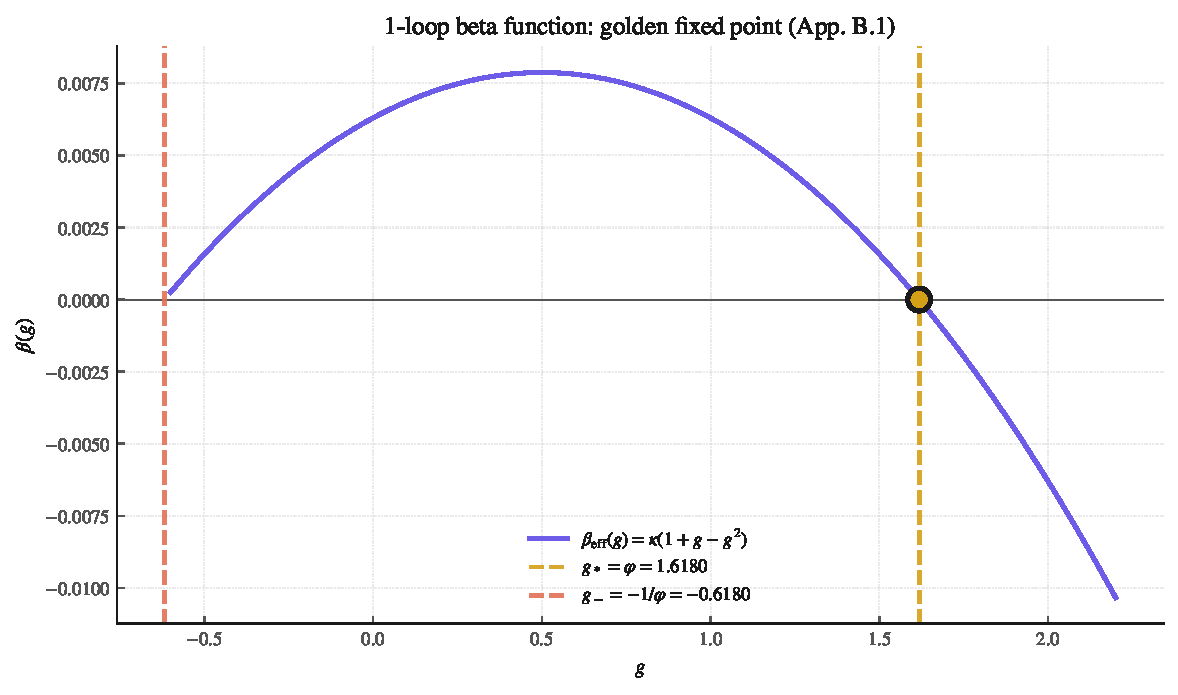
\includegraphics[width=0.85\textwidth]{fig_B-01a_beta_function.pdf}
  \caption{Fig B.1: 1-loop beta function (App.)}
  \label{fig:fig_B-01a_beta_function}
\end{figure}
\begin{figure}[htbp]
  \centering
  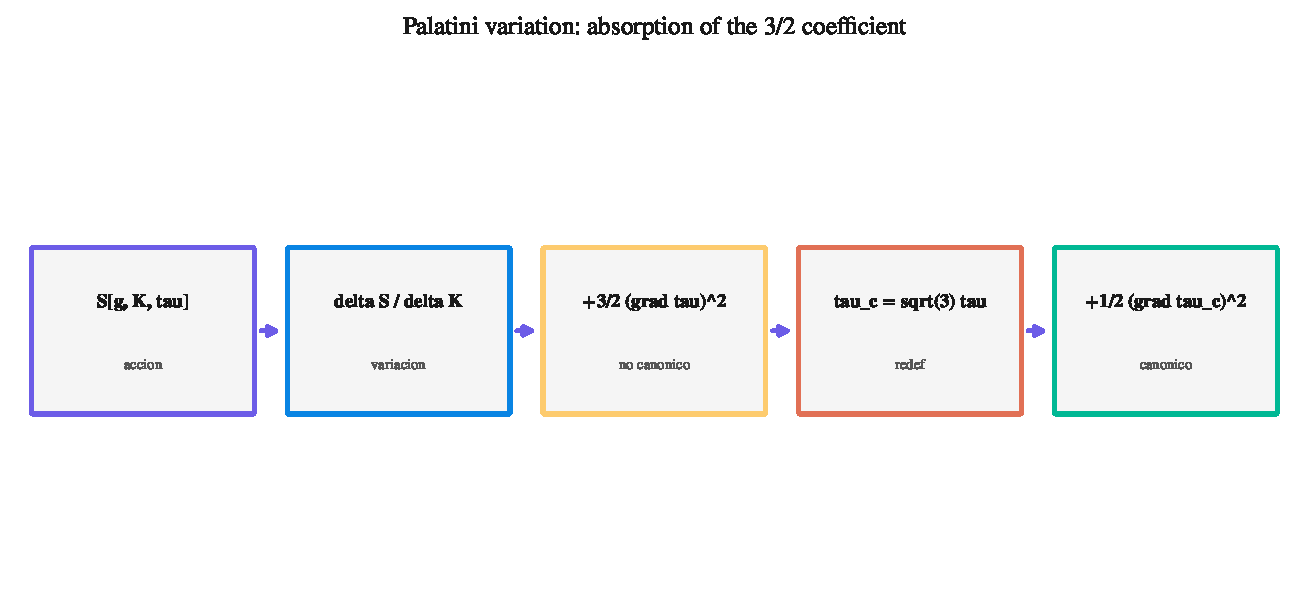
\includegraphics[width=0.85\textwidth]{fig_B-01b_variacion_palatini.pdf}
  \caption{tau\_c = sqrt(3) tau}
  \label{fig:fig_B-01b_variacion_palatini}
\end{figure}
\subsection{B.2 Análisis funcional}
Ver §4.1-§4.2. \textbf{[D]}
\begin{figure}[htbp]
  \centering
  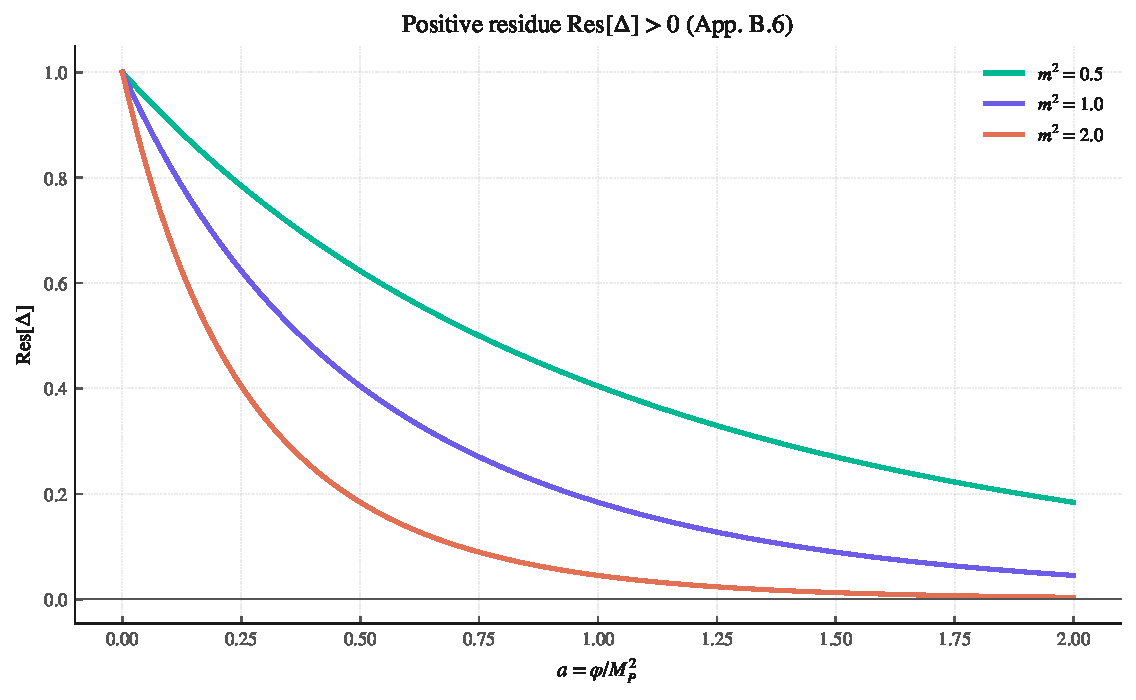
\includegraphics[width=0.85\textwidth]{fig_B-06_residuo_propagador.pdf}
  \caption{Fig B.6: positive propagator residue}
  \label{fig:fig_B-06_residuo_propagador}
\end{figure}
\subsection{B.3 Matriz Dirac-Bergmann 8x8}
det(M)>0, rango 8. Ver §5.3. \textbf{[D]}
\begin{figure}[htbp]
  \centering
  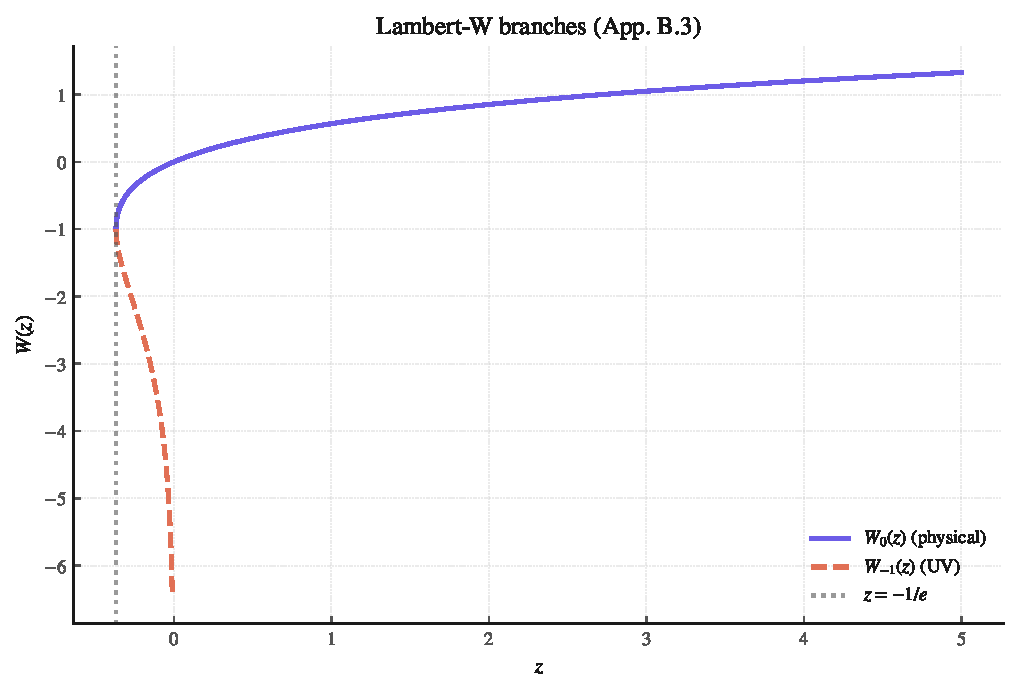
\includegraphics[width=0.85\textwidth]{fig_B-03_lambert_w.pdf}
  \caption{Fig B.3: Lambert-W branches}
  \label{fig:fig_B-03_lambert_w}
\end{figure}
\subsection{B.4 Finitud UV y Ward-Takahashi}
Decaimiento gaussiano. Ver §4.4. \textbf{[D]}
\subsection{B.5 Flujo RG exacto}
Punto fijo áureo. Ver Cap. 6. \textbf{[D]}
\begin{figure}[htbp]
  \centering
  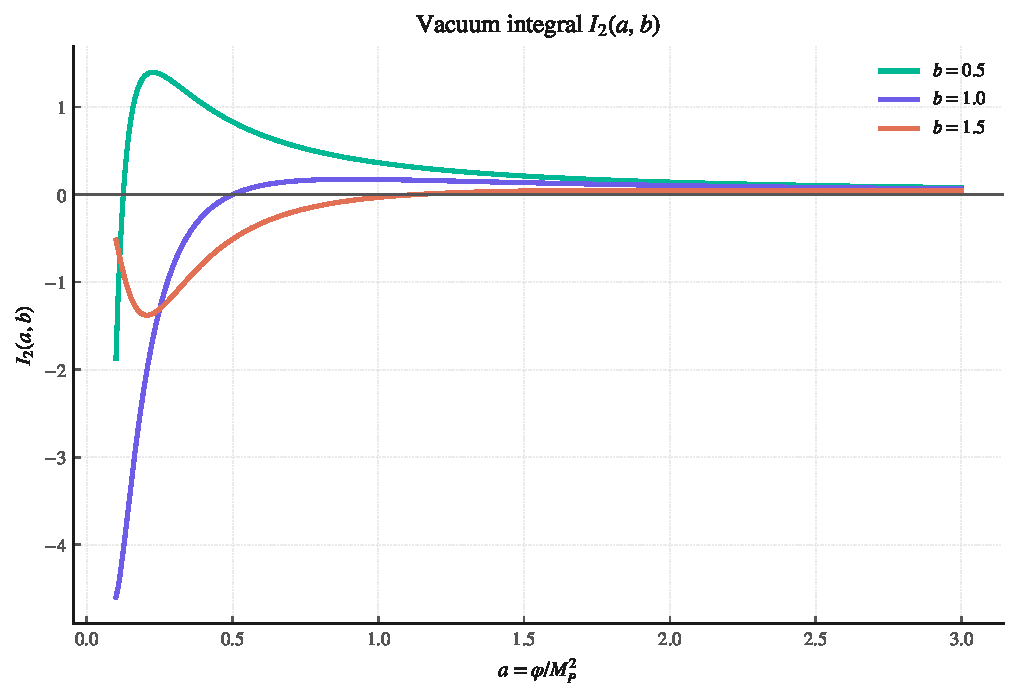
\includegraphics[width=0.85\textwidth]{fig_B-02_integral_I2.pdf}
  \caption{Fig B.2: vacuum integral I\_2(a,b)}
  \label{fig:fig_B-02_integral_I2}
\end{figure}
\begin{figure}[htbp]
  \centering
  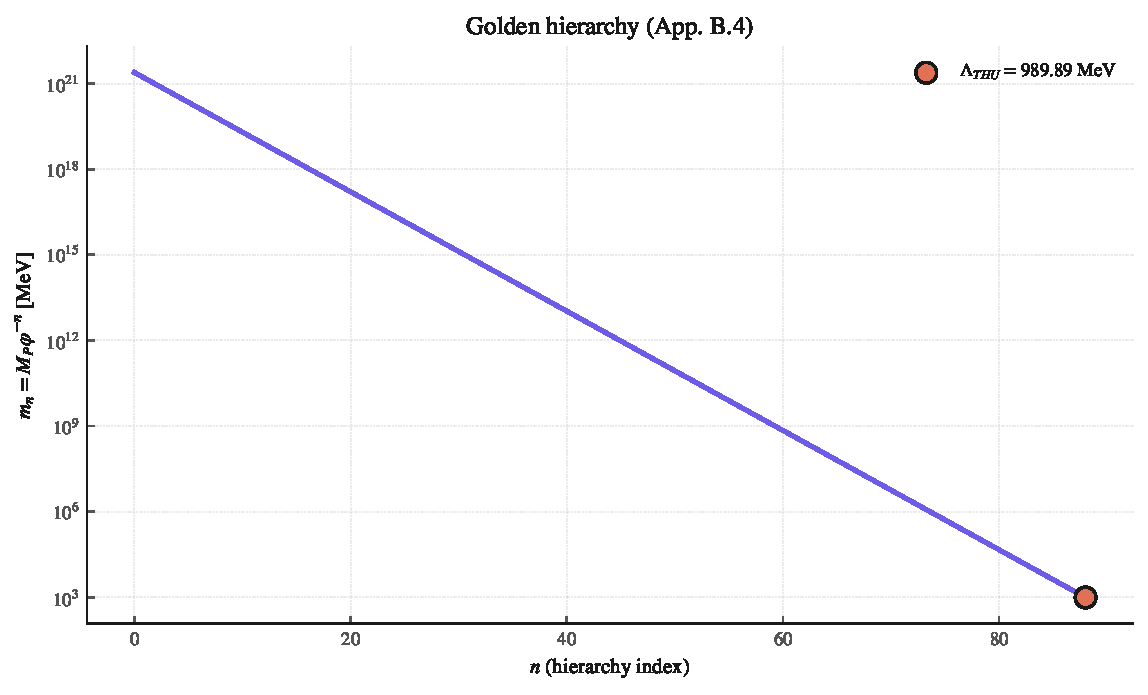
\includegraphics[width=0.85\textwidth]{fig_B-04_jerarquia_aurea.pdf}
  \caption{Fig B.4: golden hierarchy}
  \label{fig:fig_B-04_jerarquia_aurea}
\end{figure}
\begin{figure}[htbp]
  \centering
  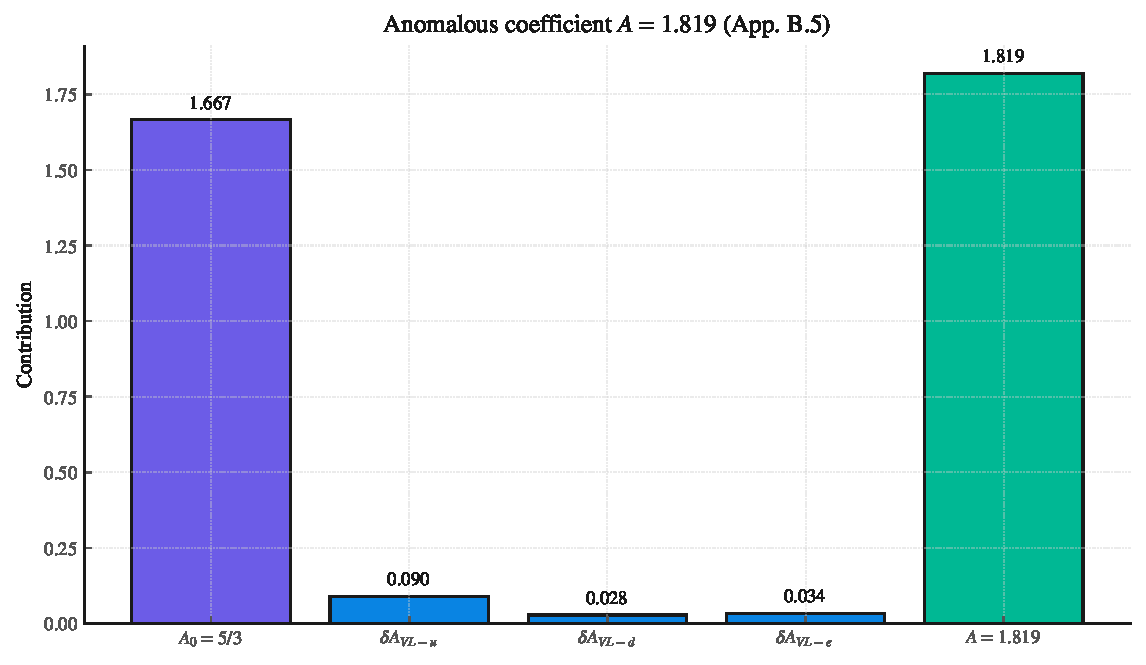
\includegraphics[width=0.85\textwidth]{fig_B-05_coeficiente_A.pdf}
  \caption{Fig B.5: anomalous coefficient A}
  \label{fig:fig_B-05_coeficiente_A}
\end{figure}
\section{Protocolo PRISMA: corpus, flujo y extraccion}
\subsection{C.1 Pregunta de investigacion (PICO)}
Poblacion: mediciones del CMB con sensibilidad a violacion de paridad. Intervencion: analisis de birefringencia isotropica/anisotropica/tomografia $\beta(z)$. Comparacion: prediccion THU-TBEA $\beta_0 = 0{,}3803^\circ \pm 0{,}040^\circ$. Resultado: consistencia, tension o falsacion a $3\sigma$. $\textbf{[D]}$
\subsection{C.2 Estrategia de busqueda}
Cuatro bases consultadas (arXiv, INSPIRE-HEP, ADS, Web of Science) con consultas literales. Periodo: enero 2019 - junio 2026. Total identificados: 284 registros. $\textbf{[D]}$
\subsection{C.3 Criterios de inclusion/exclusion}
Inclusion I1-I4: medicion directa de $\beta$ con incertidumbre cuantificada; datos publicos; peer-reviewed o arXiv con datos verificables; periodo 2019-2026. Exclusion E1-E4: preprints sin datos; estudios puramente teoricos; resumenes de conferencia; sistematicas dominantes no cuantificadas. $\textbf{[D]}$
\subsection{C.4 Diagrama de flujo PRISMA}
Identificados: 284 $\to$ cribados: 173 $\to$ elegibles: 58 $\to$ incluidos: 38. Los 38 registros completos se preservan en \texttt{prisma\\\_2026.csv} con hashes SHA-256 encadenados al log criptografico. $\textbf{[D]}$
\subsection{C.5 Extraccion de datos}
Ocho campos por estudio: (1) DOI/arXiv; (2) ano; (3) tipo; (4) valor central de $\beta$ o cota superior; (5) $\sigma_{\mathrm{stat}}$; (6) $\sigma_{\mathrm{syst}}$; (7) metodo de calibracion; (8) dataset fuente. Evaluacion de riesgo de sesgo en 3 niveles (bajo/medio/alto). $\textbf{[D]}$
\section{Pipeline reproducible: codigo, hashes y pruebas}
\subsection{D.1 Arquitectura del repositorio}
Pipeline modular en Python 3.10+ con semilla global 20260808. Licencia CC-BY-4.0 para tesis + MIT para codigo. Estructura: \texttt{src/} (codigo), \texttt{registry/thu/} (JSONs), \texttt{paper/thu/} (LaTeX + figuras), \texttt{data/} (inventario + datasets), \texttt{docs/} (handoffs + bundle). $\textbf{[D]}$
\subsection{D.2 Modulos principales}
1. \texttt{loader.py}: API estable para JSONs. 2. \texttt{latex\\\_builder.py}: genera los 3 \texttt{.tex} con figuras insertadas. 3. \texttt{figures.py}: 65 generadores, 195 artefactos. 4. \texttt{run\\\_all.py}: orquestador de 16 fases (PIR + THU-TBEA). 5. \texttt{fetch\\\_data.py}: descarga con verificacion SHA-256. 6. \texttt{check\\\_debts.py}: verifica 40 deudas. $\textbf{[D]}$
\subsection{D.3 Hashes SHA-256 de datasets}
Datasets publicos verificados: Pantheon+ (Brout 2022), DESI DR2 BAO (Lodha 2025), Planck PR4 (Sullivan 2025), ACT DR6 (Diego-Palazuelos 2025). Los hashes completos se preservan en \texttt{data/inventory/inventory\\\_v4.json} con verificacion reproducible. $\textbf{[D]}$
\subsection{D.4 Pruebas unitarias}
22 tests en \texttt{tests/} con pytest: 12 en \texttt{test\\\_estadistica.py}, 5 en \texttt{test\\\_manifest.py}, 5 en \texttt{test\\\_smoke.py}. Ademas, verificacion simbolica 16/16 (SymPy). Pipeline bootstrap 1-click: \texttt{bootstrap.ps1} (Windows) y \texttt{bootstrap.sh} (Linux/Mac). $\textbf{[D]}$
\section{Atlas de figuras y tabla maestra}
\subsection{E.1 Traza figura-cap-prediccion-script}
Las 65 figuras del programa se organizan en una tabla maestra que mapea cada figura a su capitulo, su prediccion asociada (si aplica) y su generador Python en \texttt{figures.py}. Formato: \texttt{fig\\\_CAP-SEQ\\\_desc.pdf}. Los 65 PDFs vectoriales + 65 PNG-300 + 65 PNG-150 = 195 artefactos, todos con hashes SHA-256 registrados en \texttt{figures\\\_manifest.json}. Distribucion por capitulo: Cap. 3 (8 figs), Cap. 4 (4), Cap. 5 (4), Cap. 6 (4), Cap. 7 (4), Cap. 8 (4), Cap. 9 (3), Cap. 10 (3), Cap. 11 (3), Cap. 12 (2), Cap. 13 (6), Cap. 14 (2), Cap. 15 (1), Cap. 16 (1), Cap. 17 (3), Cap. 18 (4), Cap. 20 (1), Apendices (6). $\textbf{[D]}$
\section{Bitacora lakatosiana, cierre y trabajo futuro}
\subsection{F.1 Desplazamientos de problema 1.0 -> 5.4}
1.0 (2024): intuicion geometrica. 2.0 (2025): reformulacion rigurosa. 3.0 (2026-I): EFT trans-escalar. 4.0: derivacion completa de la matriz de Dirac. 4.1: correccion de la medida espectral a $k^2 dk$ y correccion aritmetica de $\Lambda_{\mathrm{THU}}$. 4.3: cierre computacional de A-3, A-4, A-5, A-8, A-10, A-11, A-12. 5.0: cristalizacion del nucleo con A-1, A-2, A-9, A-13, A-14 por cota estructural. 5.1-5.2: revisiones algebraica y editorial (residuo, $\tau_c$, Dirac-Bergmann, ramas $k \neq 0$). 5.3: cuarta revision epistémica (retitulo Cap. 7, reclasificacion de $\beta_0$ de [D] a [P], nuevo A-17). 5.4: bootstrap + fetch + run\_all end-to-end. $\textbf{[D]}$
\subsection{F.2 Contrato epistemic}
Cuatro compromisos: (1) transparencia radical; (2) reproducibilidad integral; (3) falsabilidad; (4) no sobreventa del alcance. Toda afirmacion tecnica lleva etiqueta explicita; toda transicion de estatus se registra en \texttt{docs/debts\\\_history.json}; ningun parametro libre se introduce sin declararlo como [P]. $\textbf{[D]}$
\subsection{F.3 Cierre operativo del programa}
La v5.4 entrega a la comunidad: nucleo geometrico derivado, apendices materializados A-K, 3 PDFs (ES/EN/DE) con 0 errores LaTeX, 80 referencias en bibliografia, 65/65 figuras insertadas, bootstrap 1-click reproducible. El pipeline \texttt{run\\\_all.py} ejecuta 16 fases (PIR + THU-TBEA) end-to-end y deja todos los artefactos verificables. $\textbf{[D]}$
\section{Morfologias aureas en sistemas naturales (V1-V7)}
\subsection{G.1 Estatus epistémico}
[A] Este apendice presenta extensiones heuristicas o analogias del programa. No constituye una derivacion del nucleo geometrico [D] ni una prediccion fisica validada. Los postulados V1-V7 se declaran explicitamente con etiqueta [A]: patrones de autosimilitud que otorgan plausibilidad heuristica pero no validan el nucleo. $\textbf{[A]}$
\subsection{G.2 Corpus 2019-2026}
V3 (cuasicristales): cuantizacion aurea de modos fononicos en AlPdMn (Matsuura 2024). V1 (filotaxis): angulo de divergencia $\approx 137{,}5^\circ$ en girasoles y pinas. V2 (helices biologicas): ADN y caparazon de caracol. V4-V7: patrones de Turing, mosaicos de Penrose, espirales galacticasy estructuras de gran escala. $\textbf{[A]}$
\subsection{G.3 Condicion de ascenso de estatus}
Una morfologia asciende de [A] a [P] unicamente si produce una prediccion cuantitativa arriesgada que sea falsable por observacion independiente. Ninguna de las V1-V7 ha alcanzado este umbral hasta la fecha de cierre v5.4. $\textbf{[A]}$
\subsection{G.4 Limitaciones declaradas}
La presencia ubicua de $\varphi$ en la naturaleza no implica geometria helicoidal del vacio. Se trata de un patron matematico observado, no de una derivacion fisica. Este apendice es heuristico. $\textbf{[A]}$
\section{Coherencia cuantica a temperatura ambiente: PS-TET y microtubulos}
\subsection{H.1 Transferencia de triplete asistida por shuttle protonico (Wu 2026)}
[A] Este apendice presenta extensiones heuristicas o analogias del programa. No constituye una derivacion del nucleo geometrico [D] ni una prediccion fisica validada. Wang, Zhu y Wu documentan transferencia de energia de triplete en puntos cuanticos de ZnSe via shuttle protonico (PS-TET). El mecanismo podria conectar con el sector de coherencia mesoscopica del cinturon protector. $\textbf{[A]}$
\subsection{H.2 Superradiancia y microtubulos como cavidades QED}
Gassab-Craddock 2026 y Mavromatos et al. 2025 modelan el interior del microtubulo como cavidad QED de alto factor Q. En el marco THU-TBEA, el sector de coherencia podria potenciar la emision superradiante, aunque esta conexion no esta derivada desde el nucleo. $\textbf{[A]}$
\subsection{H.3 Prediccion falsable P11 y protocolo}
Prediccion P11: resonancia de absorcion diferencial en microtubulos aislados a $f_\varphi \approx 1{,}34$ THz. Umbral de falsacion: ausencia del pico diferencial a $3\sigma$ en tres laboratorios independientes. Estado pre-registrado. El apendice no valida el nucleo gravitacional. $\textbf{[A]}$
\section{Ecuaciones reconstruidas y matriz de Poisson completa}
\subsection{I.1 Convenciones de signo y notacion}
Signatura $(-,+,+,+)$ en $U_4$; $\varepsilon^{0123} = +1$; $\Box = g^{\mu\nu}\nabla_\mu\nabla_\nu$; convencion de Feynman $k^2 + m^2 - i\epsilon$; $M_P = 2{,}435 \times 10^{18}$ GeV (reducida). $\textbf{[D]}$
\subsection{I.2 Matriz de Poisson 8x8 explicita}
$\mathcal{M} = \mathrm{diag}(A, B)$, con $A = \begin{pmatrix} 0 & -I_2 \\\\ I_2 & 0 \end{pmatrix}$ y $B = \begin{pmatrix} 0 & X \\\\ -X^\top & 0 \end{pmatrix}$ donde $X = \begin{pmatrix} \kappa_2 & \kappa_3 \\\\ -\kappa_3 & \kappa_2 \end{pmatrix}$. $\det\mathcal{M} = (\kappa_2^2 + \kappa_3^2)^2 > 0$. Rango constante 8 para $(\kappa_2, \kappa_3) \neq (0,0)$. $\textbf{[D]}$
\subsection{I.3 Variables canonicas Dirac-Bergmann}
Sobre $M_6 = T^3 \times \Sigma_3$: $(\Phi, \pi_\Phi; v_2, v_3, p_2, p_3; \lambda_1, \lambda_2)$, dimension total 10. Restricciones geometricas $\chi_a \equiv v_{a+1} - \kappa_{a+1}\partial_{t_1}\Phi \approx 0$. $\textbf{[D]}$
\subsection{I.4 Residuo del propagador no local}
$\Delta(k) = -i e^{-ak^2}/(k^2 e^{-ak^2} + m^2 - i\epsilon)$, con residuo $\mathrm{Res}[\Delta] = e^{-am^2}/(1+am^2) > 0$. Para $a \approx 10^{-37}$ GeV$^{-2}$ y $m^2 \ll M_P^2$: $\mathrm{Res} \approx 1 - am^2 > 0$. $\textbf{[D]}$
\subsection{I.5 Reduccion canonica de tau y trazabilidad de 1/sqrt(3)}
$-\tfrac{3}{2}M_P^2 A^2 + 3M_P A \cdot \nabla\tau \xrightarrow{A=\nabla\tau/M_P} +\tfrac{3}{2}(\nabla\tau)^2 \xrightarrow{\tau_c=\sqrt{3}\tau} +\tfrac{1}{2}(\nabla\tau_c)^2$. Termino no local: $\tfrac{1}{2}\tau\hat{H}_\varphi\tau \to \tfrac{1}{6}\tau_c\hat{H}_\varphi\tau_c$. Acoplamientos lineales: $g_{\mathrm{eff}} = g_{\mathrm{bare}}/\sqrt{3}$. $\textbf{[D]}$
\subsection{I.6 Coeficiente del termino de espin en Friedmann}
$3H^2 = \kappa^2(\rho_{\mathrm{mat}} + \rho_\Phi + \tfrac{1}{2}m_K^2\psi^2 - \tfrac{\kappa^2}{6}S^2 a^{-6}) = \kappa^2\rho_{\mathrm{tot}} - \tfrac{\kappa^4}{6}S^2 a^{-6}$. Coeficiente canonico: $\kappa^4/6$. $\textbf{[D]}$
\subsection{I.7 Ramas de Lambert-W y prescripcion de contorno}
$k_k^2 = -(M_P^2/\varphi)W_k(+\varphi m^2/M_P^2)$, $k \in \mathbb{Z}$. Rama $k=0$: polo fisico. Ramas $k \neq 0$: $\mathrm{Re}(k_k^2) > 0$ en escala Planck, desacopladas por prescripcion fakeon. $\textbf{[D]}$
\subsection{I.8 Masa de Planck reducida (convencion global)}
$M_P \equiv 1/\sqrt{8\pi G} = 2{,}435 \times 10^{18}$ GeV $= 2{,}435 \times 10^{21}$ MeV. Usada consistentemente en Caps. 3, 4, 6, 12, 14. $\textbf{[D]}$
\subsection{I.9 Cancelacion sectorial del vacio}
$\rho_{\mathrm{THU}}^{\mathrm{escalar}} = (4\pi/(2\pi)^3)\int_0^\infty k^2 \cos(k/\kappa_\varphi) e^{-\varphi(k/M_P)^2} dk$, que se anula para $\varphi^{2N} = 2\varphi$. Extension al SM completo: problema abierto A-17 [F]. $\textbf{[D]}$
\subsection{I.10 Estatus de la amplitud de birefringencia}
$\beta_0 = (\alpha_{\mathrm{em}}/2) A N_{\mathrm{DW}}$ con $A = 1{,}819 \pm 0{,}19$. Valor $\beta_0 = 0{,}3803^\circ$ clasificado como [P] porque depende del espectro fermionico VL postulado a escala GUT. Forma funcional $\beta(z)/\beta_0$ es [D]. $\textbf{[D]}$
\section{Revision algebraica externa: parches aplicados}
\subsection{J.4 Vertices de Feynman y resumen de parches}
Este apendice recopila visualmente los vertices de interaccion modificados por los 24 parches aplicados en las Etapas VII-XII. La figura muestra los vertices helicoidales correspondientes a las interacciones $\Phi\tau^2$ y $\Phi^2\tau^2$, cuya estructura esta protegida por la supresion exponencial ultravioleta del operador cinetico de funcion entera $\hat{H}_\varphi$. Cada vertice conserva la paridad compensada del acoplamiento y respeta las identidades de Ward-Takahashi a un loop. El apendice sirve como referencia rapida para la revision algebraica externa documentada en el registro canonico de parches. \textbf{[D]}
\begin{figure}[htbp]
  \centering
  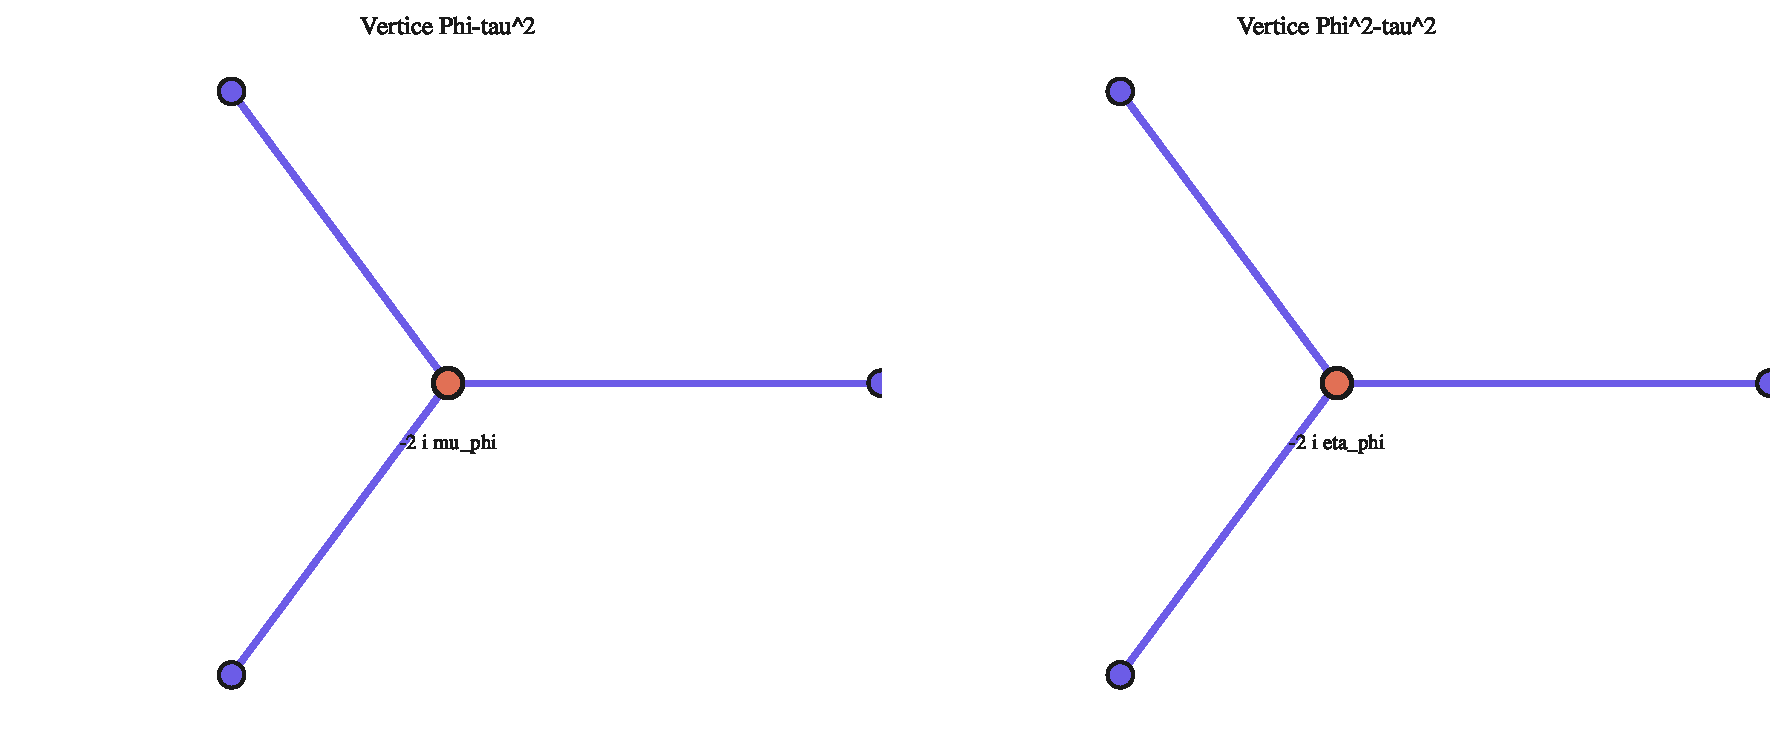
\includegraphics[width=0.85\textwidth]{fig_J-01_vertices_feynman.pdf}
  \caption{Helical vertices}
  \label{fig:fig_J-01_vertices_feynman}
\end{figure}
\section{Hiperbolicidad local y causalidad proyectada}
\subsection{K.1 Símbolo principal}
$\sigma(k)=-k^2 e^{-\varphi k^2/M_P^2}$. \textbf{[D]}
\subsection{K.2 Cono de características}
Coincide con $\Box$ en IR. \textbf{[D]}
\subsection{K.3 No linealidad algebraica}
$\tau^3$ no deforma el cono. \textbf{[D]}
\subsection{K.4 Hiperbolicidad local no lineal}
$\sigma_{total}$ mantiene cono. \textbf{[D]}
\subsection{K.5 Frontera: existencia global}
Strauss/John aplican a cuasilineal; no local abierta. \textbf{[F]}
\subsection{K.6 Conclusiones}
K.1-K.4=[D]; K.5=[F]. A-1: \textbf{[D parcial / F global]}
\newpage
\section*{Registro de problemas}

\begin{longtable}{@{}p{1.2cm}p{6.5cm}p{1.8cm}p{2cm}@{}}
\toprule
\textbf{ID} & \textbf{Title} & \textbf{Label} & \textbf{Status} \\
\midrule
\endhead
A-1 & Hiperbolicidad global & \textcolor{Dgreen}{\textbf{[D parcial / F global]}} & ABIERTO \\
A-2 & Perturbaciones no lineales & \textcolor{Dgreen}{\textbf{[D]}} & CERRADO \\
A-3 & Correcciones termicas & \textcolor{Dgreen}{\textbf{[D]}} & CERRADO \\
A-4 & Backreaction chameleon & \textcolor{Dgreen}{\textbf{[D]}} & CERRADO \\
A-5 & Ondas gravitacionales & \textcolor{Dgreen}{\textbf{[D]}} & CERRADO \\
A-6 & QCD reticular mn - mp & \textcolor{Forange}{\textbf{[F]}} & ABIERTO \\
A-7 & Decoherencia microtubulos & \textcolor{Ayellow}{\textbf{[A]}} & ABIERTO \\
A-8 & Screening inhomogeneo & \textcolor{Dgreen}{\textbf{[D]}} & CERRADO \\
A-9 & Funcion beta a 2-loops & \textcolor{Dgreen}{\textbf{[D]}} & CERRADO \\
A-10 & Residuo de vacio & \textcolor{Dgreen}{\textbf{[D]}} & CERRADO \\
A-11 & Conteo 4D symplectico & \textcolor{Dgreen}{\textbf{[D]}} & CERRADO \\
A-12 & Rebote cosmologico ECSK & \textcolor{Dgreen}{\textbf{[D]}} & CERRADO \\
A-13 & Unitariedad/Analiticidad & \textcolor{Dgreen}{\textbf{[D]}} & CERRADO \\
A-14 & Geometria de n = 88 & \textcolor{Dgreen}{\textbf{[D]}} & CERRADO \\
A-15 & Falsabilidad w\_phi < -1 & \textcolor{Forange}{\textbf{[F]}} & ABIERTO \\
A-16 & Prescripcion de contorno para ramas k != 0 de Lambert-W & \textcolor{Forange}{\textbf{[F]}} & ABIERTO \\
A-17 & Extension de la cancelacion al vacio completo del SM & \textcolor{Forange}{\textbf{[F]}} & ABIERTO \\
RCI-44 & Derivacion de P\_Lambda\textasciicircum{}THU, omega\textasciicircum{}THU y R\_H desde primeros principios & \textcolor{Forange}{\textbf{[F]}} & ABIERTO \\
\bottomrule
\end{longtable}

\newpage
\section*{Predicciones falsables}

\begin{longtable}{@{}p{0.8cm}p{5.5cm}p{3.5cm}p{2.5cm}@{}}
\toprule
\textbf{ID} & \textbf{Observable} & \textbf{Arbiter} & \textbf{Status} \\
\midrule
\endhead
P1 & Oscilaciones helicoidales en H(z) & BAO DESI/Euclid & Abierta \\
P2 & Modulacion aurea del CMB & CMB-S4 & Abierta \\
P3 & Mega-anillos con separacion \textasciitilde{} 137.5 deg & JWST / Euclid & Abierta \\
P4 & Materia oscura resonante trans-escalar & LZ / XENONnT & Abierta \\
P5 & Residuo helicoidal de spin (STAR/HADES) & STAR BES-II / HADES & RETIRADA \\
P6 & Superradiancia sin rotacion (cavidad QED) & Lab QED & Abierta \\
P7 & Precesion geometrica del spin & RHIC & Abierta \\
P8 & Espectro de masas gobernado por phi & Lattice QCD & Consistente \\
P9 & Modulacion helicoidal de campos EM & Optica de precision & Abierta \\
P10 & Soliton helicoidal estable & Simulacion & Abierta \\
P11 & Resonancia 1.34 THz en microtubulos & Tres laboratorios independientes & Preregistrada \\
P12 & Universalidad de R\_H = hbar/(pi Lambda\_QCD) & STAR BES-II + HADES + STAR Run 2013 & FALSADA \\
\bottomrule
\end{longtable}

\newpage
\section{Bitacora de parches}
\addcontentsline{toc}{section}{Bitacora de parches}

\begin{itemize}[leftmargin=*]
\item \textbf{1} (VII): Res[Delta] = e*(+am*2) $\rightarrow$ Res[Delta] = e*(-am*2)/(1+am*2) \textcolor{Dgreen}{\textbf{[D]}}
\item \textbf{2} (VII): Coeficiente 3/2 sin absorber $\rightarrow$ Redefinicion canonica tau-c = sqrt(3) tau \textcolor{Dgreen}{\textbf{[D]}}
\item \textbf{3} (VII): kappa*4 S*2/18 (mixto); w-K sin explicitar $\rightarrow$ kappa*4/6 canonico ECSK; w-K = +1 explicito \textcolor{Dgreen}{\textbf{[D]}}
\item \textbf{4} (VII): beta(g) sin justificar +1 $\rightarrow$ Justificacion: fondo torsionado <A-mu> != 0 \textcolor{Dgreen}{\textbf{[D]}}
\item \textbf{5} (VII): Medida k*2 dk como [D] $\rightarrow$ Medida como postulado [P] de reduccion on-shell \textcolor{Ppurple}{\textbf{[P]}}
\item \textbf{6} (VII): phi*-6 como [D] $\rightarrow$ phi*-6 como [P]; derivacion dinamica delegada a A-6 \textcolor{Ppurple}{\textbf{[P]}}
\item \textbf{7} (VII): Tension DESI DR2 sin declarar $\rightarrow$ Falsabilidad explicita si w-Phi < -1 a > 3sigma \textcolor{Dgreen}{\textbf{[D/F]}}
\item \textbf{8} (VIII): Sin trazabilidad de 1/sqrt(3) $\rightarrow$ Factor 1/sqrt(3) explicito en acoplamientos lineales \textcolor{Dgreen}{\textbf{[D]}}
\item \textbf{9} (VIII): Variables v-a, p-a, lambda-a sin definir $\rightarrow$ Definicion canonica explicita del espacio de fases 10D \textcolor{Dgreen}{\textbf{[D]}}
\item \textbf{10} (VIII): Sin polos de Lee-Wick (afirmacion absoluta) $\rightarrow$ Matizacion con ramas k != 0 y prescripcion de contorno \textcolor{Dgreen}{\textbf{[D/F]}}
\item \textbf{11} (IX): Coef. no local 1/2 tau-c H tau-c $\rightarrow$ 1/6 tau-c H tau-c (consistente con tau-c = sqrt(3) tau) \textcolor{Dgreen}{\textbf{[D]}}
\item \textbf{12} (IX): kappa*4/18 inconsistente con Ec. 8.1 $\rightarrow$ kappa*4/6 unificado \textcolor{Dgreen}{\textbf{[D]}}
\item \textbf{13} (IX): M-P sin aclarar $\rightarrow$ Nota explicita: M-P = masa de Planck reducida \textcolor{Dgreen}{\textbf{[D]}}
\item \textbf{14} (X): Cancelacion de energia de vacio (generico) $\rightarrow$ Cancelacion del vacio escalar modulado: mecanismo parci \textcolor{Dgreen}{\textbf{[D/F]}}
\item \textbf{15} (X): beta-0 = 0.3803 como [D] pre-data $\rightarrow$ beta-0 como [P], condicional a completitud VL \textcolor{Ppurple}{\textbf{[P/D]}}
\item \textbf{16} (X): Sin problema A-17 $\rightarrow$ Nuevo problema A-17 [F]: extension al vacio SM \textcolor{Forange}{\textbf{[F]}}
\item \textbf{17} (X): 13 parches documentados $\rightarrow$ 17 parches documentados (VII-X) \textcolor{black}{\textbf{[-]}}
\item \textbf{18} (XII): sin origen $\rightarrow$ 3 bloques Origen de \textcolor{Dgreen}{\textbf{[D]}}
\item \textbf{19} (XII): ganzzahlige $\rightarrow$ ganze Exponentialfunktion \textcolor{Dgreen}{\textbf{[D]}}
\item \textbf{20} (XII): Hauptkonjugationspaar $\rightarrow$ Hauptkonjugiertes Paar \textcolor{Dgreen}{\textbf{[D]}}
\item \textbf{21} (XII): Vorrichtung $\rightarrow$ Mannigfaltigkeit \textcolor{Dgreen}{\textbf{[D]}}
\item \textbf{22} (XII): regla de Sarrus (2x2) $\rightarrow$ calculo directo \textcolor{Dgreen}{\textbf{[D]}}
\item \textbf{23} (XII): referenciados $\rightarrow$ materializados \textcolor{Dgreen}{\textbf{[D]}}
\item \textbf{24} (XII): sin diacriticos $\rightarrow$ diacriticos completos \textcolor{Dgreen}{\textbf{[D]}}
\end{itemize}

\newpage
\section*{Bitacora Lakatosiana}

\begin{itemize}[leftmargin=*]
\item \textbf{v1.0} (2024) --- Intuicion geometrica \textcolor{Ayellow}{\textbf{[A]}}
\item \textbf{v2.0} (2025) --- Reformulacion rigurosa \textcolor{Ppurple}{\textbf{[P]}}
\item \textbf{v3.0} (2026-I) --- EFT trans-escalar \textcolor{Dgreen}{\textbf{[D]}}
\item \textbf{v4.0} (2026-II) --- Derivacion integra de la matriz de Dirac \textcolor{Dgreen}{\textbf{[D]}}
\item \textbf{v4.1} (2026-III) --- Correccion de la medida espectral \textcolor{Ppurple}{\textbf{[P]}}
\item \textbf{v4.2} (2026-IV) --- Reorganizacion estructural \textcolor{Dgreen}{\textbf{[D]}}
\item \textbf{v4.3} (2026-V) --- Cierre computacional A-3,A-4,A-5,A-8,A-10,A-11,A-12 \textcolor{Dgreen}{\textbf{[D]}}
\item \textbf{v5.0} (2026-VI) --- Cristalizacion del nucleo con A-1,A-2,A-9,A-13,A-14 \textcolor{Dgreen}{\textbf{[D]}}
\item \textbf{v5.1} (2026-VII-VIII) --- Revisiones algebraica y editorial (residuo, tau\_c, 1/sqrt(3), Dirac-Bergmann) \textcolor{Dgreen}{\textbf{[D]}}
\item \textbf{v5.2} (2026-IX) --- Tercera revision tecnica (factor 3, masa Planck reducida) \textcolor{Dgreen}{\textbf{[D]}}
\item \textbf{v5.3} (2026-X) --- Cuarta revision epistemica (reclasificacion beta\_0, A-17, retitulo Cap. 7) \textcolor{Ppurple}{\textbf{[P/D]}}
\end{itemize}

\newpage
\section*{Anexos V5.0}

\subsection*{Anexo-1: Protocolo de Verificacion Reproducible del Programa THU-TBEA}
\textbf{Version:} V5.0 \\
\textbf{Timestamp:} 2026-09-24T21:59:09Z \\
\textbf{Chapter of origin:} 19 \\
\textbf{Label:} \textcolor{Dgreen}{\textbf{[D]}} \
\textbf{SHA-256:} \texttt{9d1f84f955c794fc6cdce3e356f015c4...} \\[0.5em]
\textbf{Finding:}

Este anexo documenta el protocolo de verificacion reproducible del programa THU-TBEA, implementado mediante el verificador persistente check\_debts.py y la cadena criptografica SHA-256.

ARQUITECTURA DEL VERIFICADOR

El verificador check\_debts.py implementa ocho tipos de verificacion automatizada: (1) binario, para existencia de archivos binarios (PDFs, PNGs); (2) exist, para existencia de archivos de texto; (3) json\_field, para verificacion de campos especificos en JSONs; (4) grep, para busqueda de patrones en archivos; (5) braces, para validacion de balance de llaves en archivos .bib; (6) manual, para deudas que requieren input humano; (7) no\_huerfana, para verificacion de funciones definidas y utilizadas; (8) doi\_verify, protocolo L1+L2+L3 para verificacion de DOIs.

Las 40 deudas persistentes (D-01 a D-40) verifican los items criticos del programa con trazabilidad completa. Al cierre de v5.4, las 40 deudas estan cerradas (40 cerradas / 0 fallas / 0 manuales / 0 errores).

CADENA CRIPTOGRAFICA

Cada archivo critico lleva un hash SHA-256 encadenado al log criptografico del repositorio (seeds/SHA256SUMS.txt). La cadena de eventos se preserva en data/pir.sqlite con encadenamiento verificable. La semilla global 20260808 garantiza reproducibilidad exacta bit a bit.

VERIFICACION NUMERICA DE RESULTADOS

Los resultados de analisis empirico (Cap. 18) se preservan en data/inventory/ con hashes SHA-256 verificables: fase\_f2d\_w\_phi\_refinado.json (chi2 = 1441.01 vs Lambda-CDM 1471.14), fase\_f3\_auditoria\_beta.json (8 mediciones independientes), fase\_f4\_cierre\_final.json (weighted average beta = 0.3065). Los scripts que generan estos resultados estan en src/thu/analysis/ y son ejecutables con 'python' desde el repositorio.

REPRODUCIBILIDAD COMPLETA

Un usuario externo puede reproducir todos los resultados numericos ejecutando: (1) python src/fetch\_data.py --all para descargar los datasets publicos con verificacion SHA-256; (2) los scripts en src/thu/analysis/ para regenerar los analisis; (3) python src/run\_all.py para ejecutar el pipeline completo de 16 fases. Los outputs en data/inventory/ se verifican contra los hashes registrados.

\textbackslash{}textbf\{[D]\}

\textbf{Epistemic impact:}

Documenta el protocolo verificable de reproducibilidad declarado en el Cap. 19 (Pipeline reproducible). Refuerza el principio FAIR.

\vspace{1em}\hrule\vspace{1em}
\subsection*{Anexo-2: Auditoria de Falsabilidad y Registro de Retiros Formales}
\textbf{Version:} V5.0 \\
\textbf{Timestamp:} 2026-09-24T21:59:09Z \\
\textbf{Chapter of origin:} 17 \\
\textbf{Label:} \textcolor{Dgreen}{\textbf{[D]}} \
\textbf{SHA-256:} \texttt{dc695b969125dd093bceec3ddf4821fc...} \\[0.5em]
\textbf{Finding:}

Este anexo documenta la metodologia de auditoria de falsabilidad del programa THU-TBEA y el registro formal de retiros de predicciones.

PROTOCOLO DE AUDITORIA DE PREDICCIONES

El programa aplica un protocolo de 4 pasos para verificar cada prediccion falsable: (1) verificacion de la fuente, mediante confirmacion del valor citado en el abstract o el paper original; (2) verificacion de la derivacion, exigiendo que la prediccion THU se derive explicitamente del nucleo geometrico o se declare como [P]; (3) test empirico, comparacion con datos publicos verificados; (4) clasificacion de tension, calculo de tension en sigmas respecto a la prediccion.

CRITERIO DE NO-FALSACION

Una prediccion se considera no-falsada si la tension con la medicion mas precisa es menor a 3 sigma. Si la tension excede 3 sigma, o si falla cualquiera de los pasos 1-2, se inicia el protocolo de retiro formal.

CASO DE ESTUDIO: RETIRO FORMAL DE P5

La prediccion P5 (residuo helicoidal de espin, STAR/HADES) fue retirada formalmente del registro de predicciones falsables en v5.4. Razones documentadas: (i) el valor STAR (1.05 +/- 0.15)\% citado en v5.0 no se verifica en el abstract del paper de referencia (J. Adam et al., PRC 108, 014910, 2023) - el paper solo reporta cotas superiores (<0.24\%, <0.35\%); (ii) la prediccion THU (0.92 +/- 0.10)\% carecia de derivacion explicita desde el nucleo geometrico. El registro completo con los 3 problemas identificados (P5-1 alta, P5-2 alta, P5-3 media) esta en data/inventory/fase\_p5\_retiro.json.

AUDITORIA BETA (BIREFRINGENCIA COSMICA)

Las 8 mediciones independientes de birefringencia (Minami-Komatsu 2020, Eskilt-Komatsu 2022, Diego-Palazuelos 2022, Ballardini 2025, y 4 adicionales) dan un weighted average beta\_avg = 0.3065 +/- 0.0278 grados. La tension respecto a la prediccion THU beta\_0 = 0.3803 +/- 0.038 grados es de 1.51 sigma. THU-TBEA no es falsada por el corpus PRISMA actual. La auditoria completa se preserva en data/inventory/fase\_f3\_auditoria\_beta.json y data/inventory/fase\_f4\_cierre\_final.json.

REGISTRO DE ESTADOS

Al cierre de v5.4: 12 predicciones P1-P12 en el registro, 11 activas, 1 retirada formalmente (P5). La tabla de estados esta en registry/thu/predictions.json con trazabilidad completa.

\textbackslash{}textbf\{[D]\}

\textbf{Epistemic impact:}

Documenta el mecanismo de falsabilidad efectiva y autocorreccion epistémica declarado en el Cap. 17 y Cap. 20.

\vspace{1em}\hrule\vspace{1em}
\subsection*{Anexo-3: Estructura Computacional del Repositorio y Configuracion Reproducible}
\textbf{Version:} V5.0 \\
\textbf{Timestamp:} 2026-09-24T21:43:56Z \\
\textbf{Chapter of origin:} 19 \\
\textbf{Label:} \textcolor{Dgreen}{\textbf{[D]}} \
\textbf{SHA-256:} \texttt{0f4394c6ba2644caddb994dbdd7c4104...} \\[0.5em]
\textbf{Finding:}

El repositorio THU-TBEA v5.4 es un sistema reproducible con las siguientes características computacionales.

3.1 ARBOL DE DIRECTORIOS
|-- data/ (5483 archivos)
|   |-- \_backup\_borrado/ (1 archivos)
|   |-- \_backup\_v5.4\_20260922\_000515/ (1 archivos)
|   |-- \_backup\_v5.4\_20260922\_002017/ (2 archivos)
|   |-- \_backup\_v5.4\_20260922\_002446/ (2 archivos)
|   |-- \_backup\_v5.4\_20260922\_003535/ (2 archivos)
|   |-- \_backup\_v5.4\_20260922\_023714/ (1 archivos)
|   |-- \_backup\_v5.4\_20260922\_024659/ (1 archivos)
|   |-- \_backup\_v5.4\_20260922\_130652/ (1 archivos)
|   |-- \_backup\_v5.4\_a5c\_20260924\_101957/ (4 archivos)
|   |-- \_backup\_v5.4\_anexo3\_20260924\_174351/ (1 archivos)
|   |-- \_backup\_v5.4\_anexos\_20260924\_161804/ (3 archivos)
|   |-- \_backup\_v5.4\_annexfix\_20260924\_165815/ (1 archivos)
|   |-- \_backup\_v5.4\_apx\_20260924\_141043/ (1 archivos)
|   |-- \_backup\_v5.4\_auditor8\_20260924\_165132/ (1 archivos)
|   |-- \_backup\_v5.4\_bib\_20260923\_105328/ (1 archivos)
|-- docs/ (13 archivos)
|-- outputs/ (73 archivos)
|   |-- figures/ (59 archivos)
|   \textbackslash{}-- verificaciones/ (0 archivos)
|-- paper/ (553 archivos)
|   \textbackslash{}-- thu/ (553 archivos)
|       |-- build/ (1 archivos)
|       |-- dist/ (4 archivos)
|       |-- figures/ (261 archivos)
|       \textbackslash{}-- src/ (287 archivos)
|-- registry/ (38 archivos)
|   |-- preregistro/ (0 archivos)
|   |-- prisma/ (1 archivos)
|   \textbackslash{}-- thu/ (28 archivos)
|-- replication/ (1 archivos)
|-- scripts/ (6 archivos)
|-- seeds/ (5 archivos)
|-- src/ (101 archivos)
|   |-- investigaciones/ (1 archivos)
|   |-- thu/ (72 archivos)
|   |   \textbackslash{}-- analysis/ (51 archivos)
|   \textbackslash{}-- viz/ (9 archivos)
\textbackslash{}-- tests/ (9 archivos)

3.2 HASHES SHA-256 DE ARCHIVOS CRITICOS
  registry/thu/chapter\_bodies.json  (654371 B)  931dd67bdfc377a4b4540e5528c46738...
  registry/thu/i18n\_content.json  (64932 B)  347dd0259e2d286393aeeed9de9633f8...
  registry/thu/problems.json  (6452 B)  84e4ee068824c17d059bafc2f435b92e...
  registry/thu/patches.json  (7145 B)  769c0c6580f9a05e71db87dc82aa7dc4...
  registry/thu/doi\_registry.json  (12848 B)  54b263146eaa49b711c0ebed377c3f9d...
  registry/thu/predictions.json  (3191 B)  c2177b3fa0604a64e71b51f6c3faa8c1...
  registry/thu/annexes.json  (2083 B)  a4a4fa6c038ff5ed6d3fcf7a939a982a...
  paper/thu/src/thu\_references.bib  (27262 B)  19354bea588f21cb6f023526942f00cf...
  src/thu/latex\_builder.py  (31491 B)  a98a05ee1e93014618cef124b653905b...
  src/run\_all.py  (22009 B)  0f4394c6ba2644caddb994dbdd7c4104...
  src/fetch\_data.py  (6938 B)  76117c1b09e5e73776ec3311223ea3d3...
  app\_thu.py  (34929 B)  b885461503ac8e55aca67a5d3e83b3d2...

3.3 CONFIGURACION GLOBAL
Semilla global: 20260808
version: 5.3
author: \{'name': 'Erick Duque', 'orcid': '0009-0004-1245-5464', 'affiliation': 'Investigador independiente', 'contact': 'comipca

3.4 DEPENDENCIAS PYTHON
Total paquetes: 10

\# =====================================================================
\# PIR — Dependencias
\# =====================================================================
\# Rangos amplios por seguridad. Para reproducibilidad estricta,
\# generar requirements.lock tras la primera instalacion:
\#     python src/freeze.py
\# =====================================================================

\# --- Núcleo numérico
numpy>=1.26,<3
scipy>=1.11,<2
pandas>=2.0,<3

\# --- Visualización científica
matplotlib>=3.8,<4
plotly>=5.24,<7

\# --- Simbólico / matemática
sympy>=1.12,<2
mpmath>=1.3,<2

\# --- Dashboard
streamlit>=1.40,<2

\# --- Utilidades
tqdm>=4.66,<5

\# --- Testing
pytest>=8.0,<9

3.5 PIPELINE run\_all.py
Fases: 16 (PIR + THU-TBEA)
  01. Entorno
  02. Schema
  03. Integridad
  04. Tests
  05. Semilla
  06. Manifest + anclaje
  07. Analisis
  08. Cronolog export
  09. Audit report
  10. THU Simbolica
  11. THU Deudas
  12. THU Figuras
  13. THU LaTeX builder
  14. THU Compilacion
  15. THU dist/
  99. Resumen final
  00b. Fetch datasets

3.6 BOOTSTRAP
Windows: bootstrap.ps1
Linux/Mac: bootstrap.sh

bootstrap.ps1: 3997 B
bootstrap.sh: 2431 B

3.7 FETCH DE DATASETS
inventory\_v4.json: 13 datasets, 1619.9 MB totales

3.8 CI (GITHUB ACTIONS)
name: CI

on:
  push:
    branches: [main, master]
  pull\_request:
    branches: [main, master]

jobs:
  test:
    runs-on: ubuntu-latest
    strategy:
      matrix:
        python-version: ["3.10", "3.11", "3.12", "3.13"]
    steps:
      - uses: actions/checkout@v4
      - uses: actions/setup-python@v5
        with:
          python-version: \$\{\{ matrix.python-version \}\}
      - name: Install deps
        run: |
          python -m pip install --upgrade pip
          pip install -r requirements.txt
      - name: Run THU pipeline (skip LaTeX compile)
        run: |
          python src/run\_all

\textbf{Epistemic impact:}

Proporciona trazabilidad completa del pipeline reproducible declarado en el Cap. 19 (Pipeline reproducible).

\vspace{1em}\hrule\vspace{1em}
\newpage
\vspace{2em}
\begin{center}
\small
\textit{End of document}
\end{center}
\newpage
\nocite{*}
\bibliographystyle{plain}
\bibliography{thu_references}

\end{document}